\ifnum\aluno=1
\renewcommand\chapterillustration{abertura-vetores.jpg}
\else
\renewcommand\chapterillustration{abertura-vetores-professor.jpg}
\fi
\renewcommand\chapterwhat{Vetores no plano do ponto de vista geométrico (segmentos orientados) e algébrico (coordenadas); operações com vetores (adição, subtração e multiplicação por escalar) e suas interpretações geométricas (translação e homotetia); algumas aplicações na Física. } 
\renewcommand\chapterbecause{Vetores são os objetos matemáticos adequados para se descrever, de modo apropriado, certas grandezas (ditas vetoriais) tais como deslocamento, velocidade, aceleração e força. Mais ainda, muitas leis naturais são expressas por equações que envolvem vetores e estudar tais equações permite entender os fenômenos associados. Além disso, o material deste capítulo fornece um primeiro contato, mais simples, com uma disciplina universitária denominada Álgebra Linear, que possui várias aplicações em Biologia, Economia, Computação Gráfica, Engenharia, Física, Matemática, Química, Estatística, etc.} 


\chapter{Vetores no Plano}


\mbox{}\thispagestyle{empty}\clearpage

\thispagestyle{empty}

\begin{center}
Projeto: LIVRO ABERTO DE MATEMÁTICA

\noindent \begin{tabular}{lcccr}

\includegraphics[scale=.15]{impa}& \quad\quad& 
\includegraphics[width=3cm]{logo} & \quad\quad& 
\includegraphics[scale=.24]{obmep} 
\end{tabular}
\end{center}

\vspace*{.3cm}

Cadastre-se como colaborador no site do projeto: \url{umlivroaberto.org}

% Versão digital do capítulo:

% \url{https://www.umlivroaberto.org/BookCloud/Volume_1/master/view/GE101.html}

% \begin{center}
%   \includegraphics[width=2cm]{canvas}
% \end{center}

\begin{tabular}{p{.15\textwidth}p{.7\textwidth}}
Título: & Vetores no Plano \\
\\
Ano/ Versão: & 2021 / versão 1.0 de \today\\
\\
Editora & Instituto Nacional de Matem\'atica Pura e Aplicada (IMPA-OS)\\
\\
Realização:& Olimp\'iada Brasileira de Matem\'atica das Escolas P\'ublicas (OBMEP)\\
\\
Produção:& Associação Livro Aberto\\
\\
Coordenação: & Fabio Simas e Augusto Teixeira (livroaberto@impa.br)\\
\\
  Autores: & Humberto Bortolossi,\\
        & Lhaylla Crissaff,\\
        & Fabio Simas
\\
Revisora: &  Cydara Cavedon Ripoll  \\
          &  Letícia Rangel \\ 
\\
Design: & Andreza Moreira (Tangentes Design) \\
\\
  Ilustrações: & --- \\ 
\\
Gráficos: & --- \\
\\
  Capa: & Foto de Jr Korpa, no Unsplash \\
        & https://unsplash.com/photos/yF3S905z9dM \\

\end{tabular}

\begin{figure}[b]
\begin{minipage}[l]{5cm}
\centering

{\large Licença:}

  
\includegraphics[width=3.5cm]{cc-by-sa1}
\end{minipage}\hfill
\begin{minipage}[c]{5cm}
\centering
{\large Desenvolvido por}


\includegraphics[width=2.5cm]{logo-associacao.jpg}
\end{minipage}
\begin{minipage}[r]{5cm}
\centering

{\large Patrocínio:}
  \vspace{1em}
  
\includegraphics[width=3.5cm]{itau}
\end{minipage}
\end{figure}

\mainmatter


\begin{apresentacao}{Introdução}

\subsection{Habilidades e pré-requisitos}

Neste capítulo contempla-se a seguinte habilidade da segunda versão da \href{http://historiadabncc.mec.gov.br/documentos/bncc-2versao.revista.pdf}{Base Nacional Comum Curricular} (BNCC):

\begin{habilities}{EM11MT01}
Compreender o conceito de vetor, tanto do ponto de vista geométrico (coleção de segmentos orientados de mesmo comprimento, direção e sentido) quanto do ponto de vista algébrico, caracterizado por suas coordenadas, aplicando-o em situações da Física.
\end{habilities}

A própria BNCC dá detalhes do que se espera dessa habilidade:
\begin{quote}

O trabalho com vetores deve proporcionar aos/s estudantes, inicialmente, compreender o conceito de vetor tanto do ponto de vista geométrico (coleção de segmentos orientados de mesmo comprimento, direção e sentido) como do ponto de vista algébrico (caracterizado por suas coordenadas). Na continuidade, esse trabalho é ampliado para que eles sejam capazes de interpretar a representação geométrica da soma de vetores e da multiplicação de um vetor por um escalar e de compreender as relações entre vetores e as transformações isométricas (reflexão, translação e rotação). É importante que todo esse trabalho seja proposto de modo articulado e integrado com situações estudadas na Física, por exemplo, e com apoio de softwares de geometria dinâmica. (BNCC, 2016, p. 562)
\end{quote}

Os pré-requisitos para este capítulo são:
\begin{habilities}{EF02MA12} Identificar e registrar, em linguagem verbal ou não verbal, a localização e os deslocamentos de pessoas e de objetos no espaço, considerando mais de um ponto de referência, e indicar as mudanças de direção e de sentido.

\tcbsubtitle{EF03MA12} Descrever e representar, por meio de esboços de trajetos ou utilizando croquis e maquetes, a movimentação de pessoas ou de objetos no espaço, incluindo mudanças de direção e sentido, com base em diferentes pontos de referência.

\tcbsubtitle{EF04MA16} Descrever deslocamentos e localização de pessoas e de objetos no espaço, por meio de malhas quadriculadas e representações como desenhos, mapas, planta baixa e croquis, empregando termos como direita e esquerda, mudanças de direção e sentido, intersecção, transversais, paralelas e perpendiculares.

\tcbsubtitle{EF05MA14} Utilizar e compreender diferentes representações para a localização de objetos no plano, como mapas, células em planilhas eletrônicas e coordenadas geográficas, a fim de desenvolver as primeiras noções de coordenadas cartesianas.

\tcbsubtitle{EF05MA15} Interpretar, descrever e representar a localização ou movimentação de objetos no plano cartesiano (1º quadrante), utilizando coordenadas cartesianas, indicando mudanças de direção e de sentido e giros.

\tcbsubtitle{EF06MA20} Construir figuras planas semelhantes em situações de ampliação e de redução, com o uso de malhas quadriculadas, plano cartesiano ou tecnologias digitais.

\tcbsubtitle{EF07MA15} Realizar transformações de polígonos representados no plano cartesiano, decorrentes da multiplicação das coordenadas de seus vértices por um número inteiro.

\tcbsubtitle{EF09MA12} Reconhecer as condições necessárias e suficientes para que dois triângulos sejam semelhantes.

\tcbsubtitle{EF09MA13} Demonstrar relações métricas do triângulo retângulo, entre elas o teorema de Pitágoras, utilizando, inclusive, a semelhança de triângulos.

\tcbsubtitle{EF09MA15} Determinar o ponto médio de um segmento de reta e a distância entre dois pontos quaisquer no plano cartesiano, sem o uso de fórmulas, e utilizar esse conhecimento para calcular, por exemplo, medidas de perímetros e áreas de figuras planas construídas no plano.

\end{habilities}

Importante: antes da BNCC, o aluno do Ensino Fundamental II usualmente já tinha um contato inicial com vetores na disciplina de Ciências. Com a BNCC, pressupõe-se que é neste momento que o aluno estudará o assunto pela primeira vez.

\subsection{Tópicos que serão tratados no capítulo}
\begin{itemize}
\item {} 
Vetor do ponto de vista geométrico.
\begin{enumerate}
\item {} 
Grandezas escalares e vetoriais.

\item {} 
Vetor posição relativa no plano: orientação, módulo, notações.

\item {} 
Vetor deslocamento no plano: soma como justaposição, módulo, vetor nulo e vetor simétrico.

\item {} 
Segmentos orientados: direção, sentido e módulo.

\item {} 
Vetores como coleções de segmentos orientados de mesma direção, sentido e módulo: igualdade, soma e subtração, vetor nulo, vetor simétrico, multiplicação por número real, propriedades das operações.
\item {} 
Forças e vetores.

\end{enumerate}

\clearpage
\item {} 
Vetor do ponto de vista algébrico.
\begin{enumerate}
\item {} 
Coordenadas de um vetor no plano.

\item {} 
Interpretação geométrica da operação de multiplicação por número real: homotetias no plano.

\item {} 
Interpretação geométrica da operação de adição de vetores: translações no plano.

\item {} 
Caracterização da igualdade de vetores em termos de suas coordenadas.

\item {} 
Demonstração de algumas propriedades das operações com vetores via coordenadas.

\end{enumerate}

\end{itemize}

Não serão abordados produto escalar e produto vetorial. Vetores no espaço e, mais geralmente, vetores em \({\mathbb R}^{n}\) serão mencionados apenas na seção de aprofundamentos.

\subsection{Objetivo geral do capítulo}

Levar o estudante a perceber, seja do ponto de vista geométrico, seja do ponto de vista algébrico, a adequação do conceito de vetor no estudo de grandezas vetoriais em Física.

\subsection{Abordagem adotada no capítulo}

Vetores são normalmente estudados na disciplina de Física e, ao propor que o tópico seja estudado em Matemática, a BNCC traz uma inovação e um desafio.

A concepção deste capítulo procurou seguir de perto a orientação dada pela BNCC, a saber, desenvolver o tópico de vetores de modo articulado e integrado com situações estudadas na \textbf{Física} e com apoio de softwares de geometria dinâmica.

Nessa articulação, uma particularidade pouco evidenciada teve que ser considerada: enquanto que, tradicionalmente, em Matemática, vetores são definidos como coleções de segmentos orientados de mesma direção, sentido e módulo, de modo que se é possível operá-los a partir de qualquer um de seus representantes, dependendo da situação física em questão, nem todos os representantes são válidos e até mesmo certas operações deixam de fazer sentido. Por exemplo, na figura a seguir, se \(\overrightarrow{OA}\) e \(\overrightarrow{OB}\) são os vetores posições relativas dos pontos \(A\) e \(B\) com relação ao ponto \(O\),
apesar da soma \(\overrightarrow{OA} + \overrightarrow{OB}\) estar definida matematicamente, ela não faz sentido no contexto físico em questão (note, contudo, que a diferença \(\overrightarrow{OB} - \overrightarrow{OA}\) faz sentido: \(\overrightarrow{OB} - \overrightarrow{OA}\) é o vetor deslocamento \(\overrightarrow{AB}\)).

\begin{center}
\begin{tikzpicture}
\node [ponto] (O) at (-1.98,-0.3) {};
\node [ponto] (A) at (-1.4,2.28) {};
\node [ponto] (B) at (1.58,1.68) {};
\node [above] at (A) {$A$};
\node [above right] at (B) {$B$};
\node [below left] at (O) {$O$};
\draw [vetor] (O) -- (A);
\draw [vetor] (O) -- (B);
\end{tikzpicture}
\end{center}

Outro exemplo: no contexto de vetores deslocamentos, na figura a seguir, a soma \(\overrightarrow{AB} + \overrightarrow{CD}\) não faz sentido (pois os segmentos orientados \(\overrightarrow{AB}\) e \(\overrightarrow{CD}\) não estão justapostos), enquanto que a soma \(\overrightarrow{CD} + \overrightarrow{DE}\) faz (\(\overrightarrow{CD} + \overrightarrow{DE}\) é o vetor deslocamento \(\overrightarrow{CE}\)).

\begin{center}
\begin{tikzpicture}
\node [ponto] (A) at (-1.74,1.16) {};
\node [ponto] (B) at (-0.36,2.98) {};
\node [ponto] (C) at (3.92,0.94) {};
\node [ponto] (D) at (1.72,4.32) {};
\node [ponto] (E) at (3.92,4.9) {};
\node [below left] at (A) {$A$};
\node [above right] at (B) {$B$};
\node [below right] at (C) {$C$};
\node [above left] at (D) {$D$};
\node [above right] at (E) {$E$};
\draw [vetor] (A) -- (B);
\draw [vetor] (C) -- (D);
\draw [vetor] (D) -- (E);
\end{tikzpicture}
\end{center}

Ainda nesta linha, observe que enquanto do ponto de vista da Matemática, a "regra do triângulo"{} e a "regra do paralelogramo"{} são equivalentes para se obter a soma de dois vetores, dependendo do contexto físico, uma regra pode ser mais natural do que a outra. Por exemplo, a "regra do triângulo"{} é mais natural no contexto da soma de vetores deslocamentos, enquanto que ela é artificial no caso da soma de vetores que representam forças (uma vez que, para forças, a linha de ação da força é relevante). Reciprocamente, a "regra do paralelogramo"{} é mais natural no contexto da soma de vetores que representam forças (com todos os vetores com suas extremidades iniciais coincidentes), mas ela é artificial no contexto de vetores deslocamentos.
\begin{center}\begin{tikzpicture}
\matrix{
\coordinate (a) at (-4.45,-0.3);
\coordinate (b) at (0.89,1.68);
\coordinate (c) at (0.31,4.26);
\node [ponto] at (a) {};
\node [ponto] at (b) {};
\node [ponto] at (c) {};
\draw [vetor] (a) -- (b);
\draw [vetor] (b) -- (c);
\draw [vetor,color=destacado]  (a) -- (c);
\node [below] at ($(a)!0.5!(b)$) {$\vec{u}$};
\node [right] at ($(b)!0.5!(c)$) {$\vec{v}$};
\node [above,rotate=45,color=destacado] at ($(a)!0.5!(c)$) {$\vec{u}$ + $\vec{v}$} ;
\draw (-4.69334,-0.98342) node[anchor=north west] {Regra do Triángulo};
&
\coordinate (o) at (-1.98,-0.3);
\coordinate (a) at (-1.4,2.28);
\coordinate (b) at (1.58,1.68);
\coordinate (c) at (2.16,4.26);
\node [ponto] at (o) {};
\node [ponto] at (a) {};
\node [ponto] at (b) {};
\node [ponto] at (c) {};
\draw [vetor] (o) -- (a);
\draw [vetor] (o) -- (b);
\draw [dotted] (a)-- (c);
\draw [dotted] (b)-- (c);
\draw [vetor,color=destacado] (o) -- (c);
\node [left] at ($(o)!0.5!(a)$) {$\vec{v}$};
\node [below] at ($(o)!0.5!(b)$) {$\vec{u}$};
\node [above,rotate=45,color=destacado] at ($(o)!0.5!(c)$)  {$\vec{u}$ + $\vec{v}$} ;
\draw (-2.37284,-0.98342) node[anchor=north west] {Regra do Paralelogramo};
\\};
\end{tikzpicture}
\end{center}

Para acomodar estas particularidades, alguns livros de Física e Engenharia introduzem nomes especiais: \index{vetor fixo}vetor fixo (quando o vetor admite um único representante em uma posição específica no contexto físico), \index{vetor deslizante}vetor deslizante (quando o vetor admite qualquer representante de mesmo módulo e sentido em uma mesma reta) e \index{vetor livre}vetor livre (quando o vetor admite qualquer representante de mesmo módulo, direção e sentido em qualquer lugar do plano, ou seja, como o vetor tradicionalmente definido em Matemática). Esta terminologia já está aparecendo em livros de Matemática mais recentes usados em cursos de formação de professores (ver, por exemplo, \citet{anton2007}. Incorporar essa terminologia em sala de aula ainda é uma questão. Contudo, o mais importante, em nossa opinião, é que você tenha, antes de tudo, consciência das peculiaridades de cada caso, pois elas influenciam a maneira de como os alunos aprendem e fazem uso do conceito de vetor (conforme \citet{roche1997}).
Também é preciso ficar atento ao fato de que, muito provavelmente, esta deve ser a primeira vez que o aluno verá um símbolo usado em contexto ("\(+\)"{} para adição de números) em outro contexto ("\(+\)"{} para representar a adição de vetores).

No que se refere às grandezas físicas, optou-se pela seguinte ordem encadeada conceitualmente: posição relativa \(\rightarrow\) deslocamento \(\rightarrow\) velocidade média \(\rightarrow\) aceleração média (note que para definir aceleração média, é preciso antes definir velocidade média a qual, por sua vez, pressupõe o conceito de deslocamento e, este, pressupõe o conceito de posição relativa).

O vetor posição relativa, apesar de suas limitações (a soma deste tipo de vetor não faz sentido neste contexto), é simples e permite evidenciar para o aluno que existem grandezas que não podem ser descritas apenas com um número ou apenas como uma orientação. Assim, como primeira atividade, usamos um problema que envolve posições relativas para motivar o conceito de grandeza vetorial.
Além disso, o vetor posição relativa tem uma vantagem adicional: a escala determinada para as posições automaticamente determinar a escala do vetor, isto é, tem-se uma escala só (compare com o caso de velocidades e forças: as posições podem ter uma escala e os vetores podem ter outra completamente diferente).

Vetores deslocamentos são então introduzidos e, por meio de uma versão simplificada do jogo \textit{Corrida de Vetores} (conforme \citet{gardner1973} e \citet{oliveira2009},
\begin{itemize}
\item {} 
estabelece-se a diferença entre deslocamento e trajetória percorrida (uma confusão frequente nos alunos);

\item {} 
apresenta-se a justaposição de vetores deslocamentos a partir da qual a soma será introduzida;

\item {} 
apresenta-se o vetor deslocamento nulo e o vetor deslocamento simétrico.

\end{itemize}

Ainda com a \textit{Corrida de Vetores}, apresenta-se o uso de um segmento orientado apenas como um indicador de orientação e distância, interpretação esta que motivará a definição geral de vetor como uma coleção de segmentos orientados de mesma direção, sentido e módulo, tema da seção seguinte (\textit{Organizando as ideias}). Nesta seção, discute-se a questão dos vários significados que \textit{direção} e \textit{sentido} podem ter e qual será aquele adotado no contexto de vetores. Os conceitos de soma, vetor nulo e vetor simétrico são revisitados. Introduz-se a operação subtração e de multiplicação por um número real e algumas propriedades são então discutidas.

No lugar de conceber as coordenadas dos vetores a partir do tradicional sistema de coordenadas já apresentado e usado no Ensino Fundamental II, o tratamento de vetores do ponto de vista algébrico é conduzido como um desdobramento natural das operações de adição de vetores e multiplicação por número real que foram desenvolvidas geometricamente na seção anterior. Mais precisamente, um sistema de coordenadas é construído a partir da percepção que, fixados dois vetores não paralelos num plano, digamos \(\vec{u}\) e \(\vec{v}\), qualquer vetor \(\vec{w}\) do plano pode ser representado pelo par de números \(a\) e \(b\) tais que \(\vec{w}=a \cdot \vec{u}+b \cdot \vec{v}\). Assim, com essa nossa escolha, vetores determinam sistemas de coordenadas e não o contrário. Essa abordagem tem a vantagem de levar naturalmente a sistemas não ortogonais e de ser um primeiro contato com a leitura de certos problemas geométricos via combinações lineares (por exemplo, resolver um sistema linear \(2\,a + 3\,b = 4\) e \(5\,a - 8\,b = 7\) pode ser interpretado como encontrar os pontos de interseção das retas cujas equações são \(2\,a + 3\,b = 4\) e \(5\,a - 8\,b = 7\) ou, dualmente, determinar números reais \(a\) e \(b\) tais que \(\vec{w} = a \cdot \vec{u} + b \cdot \vec{v}\), onde \(\vec{u} = (2, 5)\), \(\vec{v} = (3, -8)\) e \(\vec{w} = (4, 7)\)).

Uma vez estabelecido o fato de que se \((a, b)\) são as coordenadas de um ponto \(P\) com relação a um sistema de coordenadas com origem \(O\), então o vetor posição relativa \(\overrightarrow{OP}\) também tem coordenadas \((a, b)\) com relação a este sistema de coordenadas, optou-se por identificar pontos com vetores desta maneira: \(P = \overrightarrow{OP}\). Com isto, a soma \(P + \vec{v}\) de um ponto com um vetor deve ser interpretada como a soma \(\vec{OP} + \vec{v}\) de vetores. Esta formulação será especialmente útil na interpretação de translações por meio de soma de vetores. Em particular, mostra-se que dado um ponto \(P=(x,y)\) e um vetor \(\vec{v}=(c,d)\), as coordenadas da translação de \(P\) por \(\vec{v}\) são \(P'=P+\vec{v} = (x,y) + (c,d) = (x+c,y+d)\) e, mais geralmente, mostra-se que se os vetores \(\vec{u}\) e \(\vec{v}\) se expressam como \(\vec{u}=(a,b)\) e  \(\vec{v} = (c, d)\) num sistema de coordenadas, então \(\vec{u} + \vec{v} = (a + c, b + d)\).

A operação de multiplicação de um vetor por um número real é interpretada geometricamente no contexto de homotetias. Aqui, usando-se semelhança de triângulos e como uma consequência da definição geométrica dada para a multiplicação de um vetor por um número real, justifica-se que se \((a, b)\) são as coordenadas de um vetor no plano e \(c\) é um número real, então \(c \cdot (a, b) = (c \cdot a, c \cdot b)\), ou seja, que esta igualdade é uma consequência e não uma definição.

Na sequência, coordenadas de vetores são usadas para justificar algumas das propriedades das operações da adição de vetores e multiplicação por um número real (comutatividade, associatividade, distributividade) mostrando que estas propriedades se reduzem às propriedades análogas para os números reais.

Por fim, desenvolve-se o uso de vetores no contexto de forças. As atividades propostas (que incluem decomposições de forças) têm como base a primeira lei de Newton interpretada da seguinte maneira: "a força resultante sobre um corpo é zero se, e somente se, sua velocidade é constante". Nesta parte, seguindo a orientação de \citet{roche1997}, em soma de forças, o vetor que representa a força resultante é sempre desenhado com uma cor diferente dos vetores que representam as forças parcelas pois, segundo o autor, é um erro comum os estudantes confundirem a força resultante como mais uma força parcela e não como uma força equivalente às forças dadas.

Registramos aqui uma analogia que pode ser útil para uma reflexão sobre o ensino e a aprendizagem de vetores: este tópico tem muito em comum com tópico dos números racionais. Seguem alguns exemplos que ilustram essa analogia.
\begin{enumerate}
\item {} 
Números racionais são classes de equivalência de frações;  vetores são classes de equivalência de segmentos orientados.

\item {} 
Existem várias "interpretações"{} para frações, cada uma com suas particularidades: parte-todo, divisão, razão, medida, operador; vetores também têm suas "interpretações", cada uma com suas particularidades: posição, deslocamento, velocidade, aceleração, força, torque.

\item {} 
A "igualdade"{} de frações se dá estabelecendo-se um critério: duas frações são iguais se elas expressam a mesma quantidade (dividir um bolo em duas partes e tomar uma parte é um processo diferente de dividir o mesmo bolo em quatro partes e tomar duas partes mas, nos dois processos, a quantidade de bolo tomada é a mesma); a "igualdade"{} de segmentos orientados também se dá por um critério: eles são iguais se possuem a mesma direção, módulo e sentido (ir 10 km para o norte saindo de Manaus não é o mesmo que ir 10 km para o norte saindo do Rio de Janeiro, pois as posições iniciais em cada caso são diferentes mas, nos dois processos, caminhou-se 10 km para o norte).

\item {} 
Existe uma flexibilidade no rigor (um "abuso de linguagem") ao se referenciar números racionais como, por exemplo, dizer  "o número racional \(2/4\)"{} ao invés de dizer "o número racional cujo representante é a fração \(2/4\)"); esta flexibilidade também ocorre com vetores: dizer "o vetor \(\overrightarrow{OP}\)"{} ao invés de dizer "o vetor cujo representante é o segmento orientado \(\overrightarrow{OP}\)".

\end{enumerate}

\subsection{Observações metodológicas gerais}
\begin{itemize}
\item {} 
As seções sob o título "Para reflexão"{} podem ser usadas de duas maneiras: (1) você pode, oralmente, na sala de aula, levantar as questões apontadas nestas seções e, então, articular uma discussão oral conjunta com os alunos ou (2) pedir para que eles, numa reflexão mais individual, leiam o texto e registrem primeiro suas respostas no caderno (funcionando, assim, como uma atividade em sala de aula) para depois fazer um fechamento acerca das questões abordadas.

\item {} 
Caso haja a disponibilidade de um projetor multimídia acoplado a um computador, \textit{tablet} ou \textit{smartphone}, você pode considerar o uso das várias atividades interativas que estão indicadas ao longo do texto. Estas atividades permitem realizar animações e   múltiplos exemplos que ajudam muito na consolidação das ideias em conceitos.

\end{itemize}
\end{apresentacao}

\def\currentcolor{session1}
\begin{objectives}{Resgate na Antártida}
{
\begin{itemize}
\item {} 
Reconhecer que a posição relativa de um ponto com relação a um outro ponto de referência é uma grandeza vetorial.

\item {} 
Reconhecer que a posição relativa depende da escolha do ponto de referência.

\end{itemize}
}{1}{1}
\end{objectives}
\begin{answer}{Resgate na Antártida}
{
\paragraph{Parte I}
\begin{enumerate}
\item {} 
Não, pois existem infinitos pontos no mapa cuja distância até a estação de pesquisa \(A\) é 10 km.

\item {} 
A circunferência de centro em \(A\) e raio 10 km.

\end{enumerate}

\begin{figure}[H]
\centering

\fbox{\noindent\includegraphics[width=225bp, trim=5mm 5mm 5mm 5mm, clip]{{geometria-vp-resposta-01}.jpg}}
\end{figure}
}{1}
\end{answer}

\begin{answer}{Resgate na Antártida}
{
\paragraph{Parte II}
\begin{enumerate}
\item {} 
Não, pois exitem infinitos pontos à nordeste da estação de pesquisa \(A\).

\item {} 
A semirreta com origem em \(A\) na direção nordeste excluindo-se \(A\).

\begin{figure}[H]
\centering

\fbox{\includegraphics[width=225bp, trim=5mm 5mm 5mm 5mm, clip]{{geometria-vp-resposta-02}.jpg}}
\end{figure}

\item {} 
Não, pois existem duas possibilidades para a localização de \(P\).

\begin{figure}[H]
\centering

\fbox{\includegraphics[width=225bp, trim=5mm 5mm 5mm 5mm, clip]{{geometria-vp-resposta-03-01}.jpg}}
\end{figure}

\begin{figure}[H]
\centering

\fbox{\includegraphics[width=225bp, trim=5mm 5mm 5mm 5mm, clip]{{geometria-vp-resposta-03-02}.jpg}}
\end{figure}

\end{enumerate}
}{9}
\end{answer}
\clearmargin
\begin{answer}{Resgate na Antártida}
{
\paragraph{Parte III}
\begin{enumerate}
\item {} 
Sim, pois existe um único ponto à nordeste de \(A\) cuja distância a \(A\) é igual a 10 km.

\item {} 
Um ponto.

\begin{figure}[H]
\centering

\fbox{\includegraphics[width=225bp, trim=5mm 5mm 5mm 5mm, clip]{{geometria-vp-resposta-04}.jpg}}
\end{figure}

\item {} 
A base \(A\) está situado à 10 km à sudoeste de \(P\).

\end{enumerate}

\paragraph{Parte IV}
\begin{enumerate}
\item {} 
O grupo \(P\) está situado à \(10 \, \sqrt{2}\) km à leste de \(B\).

\begin{figure}[H]
\centering

\fbox{\includegraphics[width=225bp, trim=5mm 5mm 5mm 5mm, clip]{{geometria-vp-resposta-05}.jpg}}
\end{figure}

\item {} 
A estação \(A\) está mais próxima.

\end{enumerate}
}{1}
\end{answer}


\explore{Vetores Posições Relativas}
\label{vetores-exp1}

\begin{task}{resgate na Antártida}
\label{ativ-vetores-vetor-posicao-relativa}



A figura a seguir exibe um mapa onde o pontorepresenta a localização de uma estação de pesquisa \(A\) na Antártida.

\begin{figure}[H]
\centering

\fbox{\includegraphics[width=250bp, trim=5mm 5mm 5mm 5mm, clip]{{geometria-vp-01}.jpg}}
\end{figure}

Um problema de localização.

\paragraph{Parte I}

A estação de pesquisa \(A\) recebe um comunicado de um avião de reconhecimento informando que um grupo \(P\) de exploradores  situado à 10 km de \(A\) necessita de socorro urgente.
\begin{enumerate}
\item {} 
É possível marcar no mapa a localização do grupo \(P\) de exploradores? Justifique sua resposta!

\item {} 
Se você marcasse no mapa todos os pontos onde o grupo \(P\) de exploradores poderia estar, que figura geométrica seria desenhada?

\end{enumerate}

\paragraph{Parte II}

Considere agora esta outra situação. A estação de pesquisa \(A\) recebe um comunicado de um avião de reconhecimento informando que um outro grupo \(Q\) de exploradores situado à nordeste de \(A\) necessita de socorro urgente.
\begin{enumerate}
\item {} 
É possível marcar no mapa a localização do grupo \(Q\) de exploradores? Justifique sua resposta!

\item {} 
Se você marcasse no mapa todos os pontos onde o grupo \(Q\) de exploradores poderia estar, que figura geométrica seria desenhada?

\item {} 
Se a estação de pesquisa \(A\) e os dois grupos de pesquisa \(P\) e \(Q\) estiverem alinhados (isto é, pertencessem a uma reta), seria possível marcar a localização do grupo \(P\) de exploradores? Justifique sua resposta!

\end{enumerate}

\paragraph{Parte III}

O avião de reconhecimento atualizou as informações sobre o grupo \(P\) de exploradores: ele está situado à 10 km à nordeste de \(A\).
\begin{enumerate}
\item {} 
É agora possível marcar no mapa a localização do grupo \(P\) de exploradores? Justifique sua resposta!

\item {} 
Nessa nova situação, se você marcasse no mapa todos os pontos onde o grupo \(P\) de exploradores poderia estar, que figura geométrica seria desenhada?

\item {} 
Caso a resposta ao Item a) seja afirmativa, com você descreveria a posição da base \(A\) com relação ao grupo \(P\) de pesquisadores?

\end{enumerate}

\paragraph{Parte IV}

Uma segunda estação de pesquisa \(B\) está situada à 10 km a noroeste de \(A\).
\begin{enumerate}
\item {} 
Considerando os dados da Parte III, como você informaria a posição do grupo \(P\) de exploradores com relação à estação \(B\)?

\item {} 
Qual estação de pesquisa está mais próxima do grupo de exploradores? \(A\) ou \(B\)? Justifique sua resposta!

\end{enumerate}
\end{task}





\paragraph{Grandezas escalares e vetoriais}

Em Física, existem grandezas que ficam perfeitamente descritas por um número e uma unidade. Este é o caso, por exemplo, do tempo, da temperatura, da pressão e da massa.
Grandezas deste tipo são denominadas \index{grandezas escalares}grandezas escalares.

Por outro lado, como você deve ter percebido com a atividade anterior, um único número não basta para especificar completamente uma posição com relação a um ponto de referência. Além da distância entre o ponto de referência e a posição em questão (no caso da atividade, "10 km"), também é necessário ter uma orientação (no caso da atividade, "à nordeste"). Grandezas físicas deste tipo \textendash{} as quais, para serem perfeitamente descritas, necessitam de um valor numérico, uma unidade e uma orientação \textendash{} são denominadas \index{grandezas vetoriais}grandezas vetoriais.

\begin{reflection}

Quais outras grandezas físicas você conhece? Elas são grandezas escalares ou vetoriais?
\end{reflection}

\clearpage

\begin{sugestions}{}
{
Sugerimos o uso da construção GeoGebra disponível no endereço \href{https://www.geogebra.org/m/kCMtPW5x/}{https://www.geogebra.org/m/kCMtPW5x} com a qual é possível mudar a posição do ponto de referência \(B\)  e, com isto, ilustrar dinamicamente para o aluno como o vetor posição relativa depende da escolha do ponto de referência.

\begin{figure}[H]
\centering

\noindent\includegraphics[width=50bp]{{ggb-vpr-01-qr}.png}
\end{figure}

\begin{marginfigure}[H]
\centering
\capstart

\noindent\includegraphics[width=300bp]{{ggb-vpr-01}.jpg}
\caption{\url{https://www.geogebra.org/m/kCMtPW5x/}.}\label{\detokenize{GE101-0:fig-ggb-vpr-01}}\label{\detokenize{GE101-0:id8}}
\end{marginfigure}}
{1}{1}
\end{sugestions}

\paragraph{Vetor Posição Relativa}

A posição relativa, a exemplo de outras grandezas vetoriais que veremos neste capítulo, pode ser representada
geometricamente por um \index{segmento de reta orientado}segmento de reta orientado, o qual é normalmente desenhado como uma seta.
Este tipo de representação para a posição relativa será denominada \index{vetor posição relativa}vetor posição relativa.
A figura a seguir exibe os vetores posições relativas do grupo de exploradores (marcado como \(G\) na figura)
com relação às estações de pesquisa \(A\) e \(B\) da atividade anterior.

\begin{figure}[H]
\centering
\capstart

\fbox{\includegraphics[width=250bp,trim=5mm 5mm 5mm 5mm, clip]{{geometria-vp-02}.jpg}}
\caption{Vetores posições relativas do ponto \(G\) determinados pelos pontos de referência \(A\) e \(B\).}
\end{figure}

\begin{reflection}

Por que posições relativas não poderiam ser representadas apenas com segmentos de reta? Por que usar segmentos orientados é importante neste contexto?
\end{reflection}

\paragraph{Notações}

Ao fazer referência a um vetor posição relativa, no lugar de uma descrição longa do tipo "vetor posição relativa do ponto \(G\) com relação ao ponto de referência \(A\)", é costume introduzir notações que permitem referenciar o vetor posição relativa de forma mais curta (essa \textit{economia} de escrita é uma prática comum na Matemática). Por exemplo, uma das notações adotada para representar o "vetor posição relativa do ponto \(G\) com relação ao ponto de referência \(A\)"{} é \(\overrightarrow{AG}\). Nesta notação, ao lê-la da esquerda para direita, a primeira letra representa o ponto de referência (no caso, o ponto \(A\)) e a segunda letra representa a posição em consideração (no caso, o ponto \(G\)). A seta sobre as duas letras é um recurso gráfico para lembrar que a notação está representando um vetor. Neste contexto, o ponto \(A\) é denominado \index{extremidade inicial}extremidade inicial (ou simplesmente \index{origem}origem) e o ponto \(G\) é denominado \index{extremidade final}extremidade final (ou simplesmente \index{extremidade}extremidade, quando não há perigo de confusão com a extremidade inicial) do vetor \(\overrightarrow{AG}\). O comprimento do segmento de reta \(AG\) é denominado \index{módulo}módulo do vetor \(\overrightarrow{AG}\) e será denotado por \(|\overrightarrow{AG}|\). No caso do vetor \(\overrightarrow{AG}\) da figura seguinte (relacionada com a atividade proposta no início desta seção), tem-se
\(|\overrightarrow{AG}| = 10~\text{km}\).

Uma notação ainda mais curta é simplesmente dar um "nome"{} ao vetor posição relativa, também como uma seta em cima. Por exemplo, na figura a seguir, o vetor posição relativa \(\overrightarrow{AG}\) é denotado por \(\vec{u}\) e o vetor posição \(\overrightarrow{BG}\) é representado por \(\vec{v}\). Nesta notação mais curta, o módulo do vetor posição relativa \(\vec{v}\) é denotado por \(|\vec{v}|\). Assim,
para \(\vec{v}\) da figura seguinte (relacionada com a atividade proposta no início desta seção), tem-se
\(|\vec{v}| = 10 \, \sqrt{2}~\text{km}\) (por quê?).

\begin{figure}[H]
\centering
\capstart

\fbox{\includegraphics[width=250bp,trim=5mm 5mm 5mm 5mm, clip]{{geometria-vp-03}.jpg}}
\caption{Notação para vetores posições relativas.}
\end{figure}

\begin{observationtitle}{Observações sobre notação e terminologia}
\begin{itemize}
\item {} 
Alguns livros usam ainda um outro tipo de notação: grandezas vetoriais são representadas por letras em negrito e grandezas escalares por letras em itálico.

\item {} 
Dependendo do autor e do contexto, o módulo de um vetor também pode ser chamado de \index{magnitude}magnitude, \index{intensidade}intensidade ou \index{valor}valor.

\end{itemize}
\end{observationtitle}

Antes de prosseguirmos, é importante destacar uma característica importante do vetor posição relativa: ele depende da escolha do ponto de referência. Veja, por exemplo, na situação ilustrada na figura anterior, que a posição \(G\) é representada por vetores posições relativas diferentes quando pontos de referências diferentes (\(A\) e \(B\)) são escolhidos.


\clearpage
\begin{sugestions}{Vetores deslocamentos}
{Observe que o vetor deslocamento é definido apenas em termos dos pontos inicial e final e estes não mudam com escolhas diferentes para o ponto de referência. Por este motivo, o vetor deslocamento também não muda. Na  
\Fref{fig-geometria-deslocamento-01}, o ponto de referência \(L\) não precisa, obrigatoriamente, ser um ponto da pista.

Estudos educacionais mostram que os alunos têm a forte tendência em confundir vetor deslocamento com trajetória. No sentido de minimizar o efeito deste distrator, sugerimos o uso da construção GeoGebra disponível no endereço \url{https://www.geogebra.org/m/f8GCVdyx}. Com ela, é possível visualizar um ponto percorrendo o modelo da pista de Interlagos apresentado na  
\Fref{fig-geometria-deslocamento-01} e, ao mesmo tempo, definir diferentes vetores deslocamentos definidos por duas posições na pista. Ao, dinamicamente, confrontar a trajetória percorrida com os diversos vetores deslocamentos, espera-se criar uma imagem mental que reforce as diferenças entre os dois conceitos.

\begin{figure}[H]
\centering

\noindent\includegraphics[width=50bp]{{ggb-interlagos-01-qr}.png}
\end{figure}

% \begin{figure}[H]
% \centering
% \capstart

% % \noindent\includegraphics[width=400bp]{{ggb-interlagos-01_2}.png}
% \caption{\url{https://www.geogebra.org/m/f8GCVdyx}.}\label{\detokenize{GE101-0A:id2}}\end{figure}

Além do trabalho de uma força em Física, como mencionado no texto para o aluno, a própria velocidade média (como uma grandeza vetorial) é um conceito que é definido em termos de vetores deslocamentos apenas e não de \index{distâncias percorridas}distâncias percorridas em uma trajetória. Ao se considerar distâncias percorridas, um outro conceito é estabelecido: o de \index{rapidez média}rapidez média (\textit{speed} em Inglês), também denominada de \index{velocidade escalar média}velocidade escalar média. Assim, é importante diferenciar os dois conceitos: velocidade média (uma grandeza vetorial) e rapidez média (uma grandeza escalar).}
{1}{1}
\end{sugestions}

\explore{Vetores Deslocamentos}

Um dos objetivos da Física é estudar como certas grandezas variam no tempo. Um carro, por exemplo, ao percorrer a pista de Interlagos em São Paulo sem parar, ocupará posições diferentes em tempos diferentes, isto é, sua posição variará ao longo do tempo. Na figura a seguir, estão marcadas duas posições na pista: o ponto \(S\) que demarca a curva "S"{} do Sena (posição esta, digamos, ocupada pelo carro em um tempo inicial) e o ponto \(T\) que demarca o final do trecho da "reta oposta"{} (ocupada pelo carro em um tempo final). Também estão desenhados na figura os vetores posições relativas \(\overrightarrow{LS}\) e \(\overrightarrow{LT}\) (considerando-se, então, \(L\) como ponto de referência).
Como representar matematicamente esta variação de posição de \(S\) para \(T\)? Isto também será feito por um segmento orientado que, neste contexto, será denominada \index{vetor deslocamento} vetor deslocamento. A seta que representa o segmento orientado é desenhada com extremidade inicial na posição inicial (isto é, aquela associada ao tempo inicial) e extremidade final na posição final (isto é, aquela associado ao tempo final). As notações usadas para vetores deslocamentos são as mesmas usadas para vetores posições relativas. Assim, por exemplo, o vetor deslocamento azul na figura pode ser denotado por \(\overrightarrow{ST}\) ou \(\vec{u}\).


% \begin{figure}[H]
% \centering
% \begin{tikzpicture}[scale=.7]
% \begin{scope}[line cap=round,line join=round,>=latex,x=0.001cm,y=0.001cm,scale=4]
% \filldraw [white, fill opacity=100] (0,200) rectangle (2400,2200);
% \draw [grafica, line width=2pt] (5.04401,1280.3)-- (209.455,435.9657720937503);
% \draw[grafica, line width=2pt, smooth, samples=100, domain=0.0:1.0] plot[parametric] function{318.647*(1.0-t)**(3.0-1.0-0.0)*t**(0.0)+361.833*2.0*(1.0-t)**(3.0-1.0-1.0)*t**(1.0)+386.322*(1.0-t)**(3.0-1.0-2.0)*t**(2.0),244.11577209375037*(1.0-t)**(3.0-1.0-0.0)*t**(0.0)+239.9257720937503*2.0*(1.0-t)**(3.0-1.0-1.0)*t**(1.0)+279.9657720937503*(1.0-t)**(3.0-1.0-2.0)*t**(2.0)};
% \draw[grafica, line width=2pt, smooth, samples=100, domain=0.0:1.0] plot[parametric] function{209.455*(1.0-t)**(4.0-1.0-0.0)*t**(0.0)+221.765*3.0*(1.0-t)**(4.0-1.0-1.0)*t**(1.0)+268.521*3.0*(1.0-t)**(4.0-1.0-2.0)*t**(2.0)+318.647*(1.0-t)**(4.0-1.0-3.0)*t**(3.0),435.9657720937503*(1.0-t)**(4.0-1.0-0.0)*t**(0.0)+367.1657720937503*3.0*(1.0-t)**(4.0-1.0-1.0)*t**(1.0)+260.3257720937504*3.0*(1.0-t)**(4.0-1.0-2.0)*t**(2.0)+244.11577209375037*(1.0-t)**(4.0-1.0-3.0)*t**(3.0)};
% \draw [grafica, line width=2pt, smooth, samples=100, domain=0.0:1.0] (138.179,1855.6177720937503)-- (5.04401,1280.3367720937504);
% \draw[grafica, line width=2pt, smooth, samples=100, domain=0.0:1.0] plot[parametric] function{386.322*(1.0-t)**(4.0-1.0-0.0)*t**(0.0)+442.508*3.0*(1.0-t)**(4.0-1.0-1.0)*t**(1.0)+460.402*3.0*(1.0-t)**(4.0-1.0-2.0)*t**(2.0)+460.402*(1.0-t)**(4.0-1.0-3.0)*t**(3.0),279.9657720937503*(1.0-t)**(4.0-1.0-0.0)*t**(0.0)+353.2857720937502*3.0*(1.0-t)**(4.0-1.0-1.0)*t**(1.0)+327.1657720937503*3.0*(1.0-t)**(4.0-1.0-2.0)*t**(2.0)+327.1657720937503*(1.0-t)**(4.0-1.0-3.0)*t**(3.0)};
% \draw[grafica, line width=2pt, smooth, samples=100, domain=0.0:1.0] plot[parametric] function{460.402*(1.0-t)**(4.0-1.0-0.0)*t**(0.0)+534.808*3.0*(1.0-t)**(4.0-1.0-1.0)*t**(1.0)+707.814*3.0*(1.0-t)**(4.0-1.0-2.0)*t**(2.0)+841.606*(1.0-t)**(4.0-1.0-3.0)*t**(3.0),327.1657720937503*(1.0-t)**(4.0-1.0-0.0)*t**(0.0)+278.8157720937504*3.0*(1.0-t)**(4.0-1.0-1.0)*t**(1.0)+215.02577209375022*3.0*(1.0-t)**(4.0-1.0-2.0)*t**(2.0)+345.50577209375024*(1.0-t)**(4.0-1.0-3.0)*t**(3.0)};
% \draw[grafica, line width=2pt, smooth, samples=100, domain=0.0:1.0] plot[parametric] function{841.606*(1.0-t)**(4.0-1.0-0.0)*t**(0.0)+893.131*3.0*(1.0-t)**(4.0-1.0-1.0)*t**(1.0)+903.281*3.0*(1.0-t)**(4.0-1.0-2.0)*t**(2.0)+921.183*(1.0-t)**(4.0-1.0-3.0)*t**(3.0),345.50577209375024*(1.0-t)**(4.0-1.0-0.0)*t**(0.0)+394.49577209375025*3.0*(1.0-t)**(4.0-1.0-1.0)*t**(1.0)+481.3057720937504*3.0*(1.0-t)**(4.0-1.0-2.0)*t**(2.0)+547.9857720937503*(1.0-t)**(4.0-1.0-3.0)*t**(3.0)};
% \draw[grafica, line width=2pt, smooth, samples=100, domain=0.0:1.0] plot[parametric] function{921.183*(1.0-t)**(4.0-1.0-0.0)*t**(0.0)+938.703*3.0*(1.0-t)**(4.0-1.0-1.0)*t**(1.0)+1079.22*3.0*(1.0-t)**(4.0-1.0-2.0)*t**(2.0)+1105.64*(1.0-t)**(4.0-1.0-3.0)*t**(3.0),547.9857720937503*(1.0-t)**(4.0-1.0-0.0)*t**(0.0)+613.2357720937503*3.0*(1.0-t)**(4.0-1.0-1.0)*t**(1.0)+1134.5767720937502*3.0*(1.0-t)**(4.0-1.0-2.0)*t**(2.0)+1239.8967720937503*(1.0-t)**(4.0-1.0-3.0)*t**(3.0)};
% \draw[grafica, line width=2pt, smooth, samples=100, domain=0.0:1.0] plot[parametric] function{1105.64*(1.0-t)**(4.0-1.0-0.0)*t**(0.0)+1128.42*3.0*(1.0-t)**(4.0-1.0-1.0)*t**(1.0)+1160.75*3.0*(1.0-t)**(4.0-1.0-2.0)*t**(2.0)+1147.38*(1.0-t)**(4.0-1.0-3.0)*t**(3.0),1239.8967720937503*(1.0-t)**(4.0-1.0-0.0)*t**(0.0)+1330.6797720937502*3.0*(1.0-t)**(4.0-1.0-1.0)*t**(1.0)+1444.8177720937504*3.0*(1.0-t)**(4.0-1.0-2.0)*t**(2.0)+1475.4617720937504*(1.0-t)**(4.0-1.0-3.0)*t**(3.0)};
% \draw[grafica, line width=2pt, smooth, samples=100, domain=0.0:1.0] plot[parametric] function{1147.38*(1.0-t)**(4.0-1.0-0.0)*t**(0.0)+1107.46*3.0*(1.0-t)**(4.0-1.0-1.0)*t**(1.0)+892.385*3.0*(1.0-t)**(4.0-1.0-2.0)*t**(2.0)+843.739*(1.0-t)**(4.0-1.0-3.0)*t**(3.0),1475.4617720937504*(1.0-t)**(4.0-1.0-0.0)*t**(0.0)+1559.3737720937502*3.0*(1.0-t)**(4.0-1.0-1.0)*t**(1.0)+1584.0617720937503*3.0*(1.0-t)**(4.0-1.0-2.0)*t**(2.0)+1566.3457720937504*(1.0-t)**(4.0-1.0-3.0)*t**(3.0)};
% \draw[grafica, line width=2pt, smooth, samples=100, domain=0.0:1.0] plot[parametric] function{843.739*(1.0-t)**(4.0-1.0-0.0)*t**(0.0)+744.842*3.0*(1.0-t)**(4.0-1.0-1.0)*t**(1.0)+683.333*3.0*(1.0-t)**(4.0-1.0-2.0)*t**(2.0)+606.76*(1.0-t)**(4.0-1.0-3.0)*t**(3.0),1566.3457720937504*(1.0-t)**(4.0-1.0-0.0)*t**(0.0)+1547.6357720937503*3.0*(1.0-t)**(4.0-1.0-1.0)*t**(1.0)+1415.9157720937503*3.0*(1.0-t)**(4.0-1.0-2.0)*t**(2.0)+1305.9957720937505*(1.0-t)**(4.0-1.0-3.0)*t**(3.0)};
% \draw[grafica, line width=2pt, smooth, samples=100, domain=0.0:1.0] plot[parametric] function{606.76*(1.0-t)**(4.0-1.0-0.0)*t**(0.0)+563.092*3.0*(1.0-t)**(4.0-1.0-1.0)*t**(1.0)+417.513*3.0*(1.0-t)**(4.0-1.0-2.0)*t**(2.0)+378.175*(1.0-t)**(4.0-1.0-3.0)*t**(3.0),1305.9957720937505*(1.0-t)**(4.0-1.0-0.0)*t**(0.0)+1243.1287720937503*3.0*(1.0-t)**(4.0-1.0-1.0)*t**(1.0)+1068.8397720937503*3.0*(1.0-t)**(4.0-1.0-2.0)*t**(2.0)+1033.2157720937503*(1.0-t)**(4.0-1.0-3.0)*t**(3.0)};
% \draw[grafica, line width=2pt, smooth, samples=100, domain=0.0:1.0] plot[parametric] function{378.175*(1.0-t)**(4.0-1.0-0.0)*t**(0.0)+288.797*3.0*(1.0-t)**(4.0-1.0-1.0)*t**(1.0)+186.292*3.0*(1.0-t)**(4.0-1.0-2.0)*t**(2.0)+169.032*(1.0-t)**(4.0-1.0-3.0)*t**(3.0),1033.2157720937503*(1.0-t)**(4.0-1.0-0.0)*t**(0.0)+981.9757720937503*3.0*(1.0-t)**(4.0-1.0-1.0)*t**(1.0)+1071.3487720937503*3.0*(1.0-t)**(4.0-1.0-2.0)*t**(2.0)+1086.6437720937502*(1.0-t)**(4.0-1.0-3.0)*t**(3.0)};
% \draw[grafica, line width=2pt, smooth, samples=100, domain=0.0:1.0] plot[parametric] function{169.032*(1.0-t)**(4.0-1.0-0.0)*t**(0.0)+151.793*3.0*(1.0-t)**(4.0-1.0-1.0)*t**(1.0)+122.607*3.0*(1.0-t)**(4.0-1.0-2.0)*t**(2.0)+138.801*(1.0-t)**(4.0-1.0-3.0)*t**(3.0),1086.6437720937502*(1.0-t)**(4.0-1.0-0.0)*t**(0.0)+1101.9217720937504*3.0*(1.0-t)**(4.0-1.0-1.0)*t**(1.0)+1363.7277720937504*3.0*(1.0-t)**(4.0-1.0-2.0)*t**(2.0)+1381.6537720937504*(1.0-t)**(4.0-1.0-3.0)*t**(3.0)};
% \draw[grafica, line width=2pt, smooth, samples=100, domain=0.0:1.0] plot[parametric] function{138.801*(1.0-t)**(4.0-1.0-0.0)*t**(0.0)+174.102*3.0*(1.0-t)**(4.0-1.0-1.0)*t**(1.0)+240.937*3.0*(1.0-t)**(4.0-1.0-2.0)*t**(2.0)+309.284*(1.0-t)**(4.0-1.0-3.0)*t**(3.0),1381.6537720937504*(1.0-t)**(4.0-1.0-0.0)*t**(0.0)+1421.4877720937502*3.0*(1.0-t)**(4.0-1.0-1.0)*t**(1.0)+1314.9407720937502*3.0*(1.0-t)**(4.0-1.0-2.0)*t**(2.0)+1318.6827720937504*(1.0-t)**(4.0-1.0-3.0)*t**(3.0)};
% \draw [grafica, line width=2pt, smooth, samples=100, domain=0.0:1.0] plot[parametric] function{309.284*(1.0-t)**(4.0-1.0-0.0)*t**(0.0)+371.309*3.0*(1.0-t)**(4.0-1.0-1.0)*t**(1.0)+365.138*3.0*(1.0-t)**(4.0-1.0-2.0)*t**(2.0)+365.138*(1.0-t)**(4.0-1.0-3.0)*t**(3.0),1318.6827720937504*(1.0-t)**(4.0-1.0-0.0)*t**(0.0)+1321.1957720937503*3.0*(1.0-t)**(4.0-1.0-1.0)*t**(1.0)+1403.8567720937504*3.0*(1.0-t)**(4.0-1.0-2.0)*t**(2.0)+1403.8567720937504*(1.0-t)**(4.0-1.0-3.0)*t**(3.0)};
% \draw[grafica, line width=2pt, smooth, samples=100, domain=0.0:1.0] plot[parametric] function{365.138*(1.0-t)**(4.0-1.0-0.0)*t**(0.0)+361.754*3.0*(1.0-t)**(4.0-1.0-1.0)*t**(1.0)+356.028*3.0*(1.0-t)**(4.0-1.0-2.0)*t**(2.0)+238.092*(1.0-t)**(4.0-1.0-3.0)*t**(3.0),1403.8567720937504*(1.0-t)**(4.0-1.0-0.0)*t**(0.0)+1472.8107720937503*3.0*(1.0-t)**(4.0-1.0-1.0)*t**(1.0)+1464.6937720937503*3.0*(1.0-t)**(4.0-1.0-2.0)*t**(2.0)+1564.8117720937503*(1.0-t)**(4.0-1.0-3.0)*t**(3.0)};
% \draw[grafica, line width=2pt, smooth, samples=100, domain=0.0:1.0] plot[parametric] function{238.092*(1.0-t)**(4.0-1.0-0.0)*t**(0.0)+221.71*3.0*(1.0-t)**(4.0-1.0-1.0)*t**(1.0)+199.238*3.0*(1.0-t)**(4.0-1.0-2.0)*t**(2.0)+192.319*(1.0-t)**(4.0-1.0-3.0)*t**(3.0),1564.8117720937503*(1.0-t)**(4.0-1.0-0.0)*t**(0.0)+1585.1927720937504*3.0*(1.0-t)**(4.0-1.0-1.0)*t**(1.0)+1687.1847720937503*3.0*(1.0-t)**(4.0-1.0-2.0)*t**(2.0)+1714.9357720937503*(1.0-t)**(4.0-1.0-3.0)*t**(3.0)};
% \draw[grafica, line width=2pt, smooth, samples=100, domain=0.0:1.0] plot[parametric] function{192.319*(1.0-t)**(4.0-1.0-0.0)*t**(0.0)+179.072*3.0*(1.0-t)**(4.0-1.0-1.0)*t**(1.0)+183.119*3.0*(1.0-t)**(4.0-1.0-2.0)*t**(2.0)+218.519*(1.0-t)**(4.0-1.0-3.0)*t**(3.0),1714.9357720937503*(1.0-t)**(4.0-1.0-0.0)*t**(0.0)+1770.2777720937502*3.0*(1.0-t)**(4.0-1.0-1.0)*t**(1.0)+1796.9417720937504*3.0*(1.0-t)**(4.0-1.0-2.0)*t**(2.0)+1799.0777720937504*(1.0-t)**(4.0-1.0-3.0)*t**(3.0)};
% \draw[grafica, line width=2pt, smooth, samples=100, domain=0.0:1.0] plot[parametric] function{218.519*(1.0-t)**(4.0-1.0-0.0)*t**(0.0)+245.627*3.0*(1.0-t)**(4.0-1.0-1.0)*t**(1.0)+382.753*3.0*(1.0-t)**(4.0-1.0-2.0)*t**(2.0)+405.89*(1.0-t)**(4.0-1.0-3.0)*t**(3.0),1799.0777720937504*(1.0-t)**(4.0-1.0-0.0)*t**(0.0)+1794.1087720937503*3.0*(1.0-t)**(4.0-1.0-1.0)*t**(1.0)+1646.5287720937504*3.0*(1.0-t)**(4.0-1.0-2.0)*t**(2.0)+1631.5627720937503*(1.0-t)**(4.0-1.0-3.0)*t**(3.0)};
% \draw[grafica, line width=2pt, smooth, samples=100, domain=0.0:1.0] plot[parametric] function{405.89*(1.0-t)**(4.0-1.0-0.0)*t**(0.0)+474.532*3.0*(1.0-t)**(4.0-1.0-1.0)*t**(1.0)+569.688*3.0*(1.0-t)**(4.0-1.0-2.0)*t**(2.0)+601.081*(1.0-t)**(4.0-1.0-3.0)*t**(3.0),1631.5627720937503*(1.0-t)**(4.0-1.0-0.0)*t**(0.0)+1577.3287720937503*3.0*(1.0-t)**(4.0-1.0-1.0)*t**(1.0)+1616.5497720937503*3.0*(1.0-t)**(4.0-1.0-2.0)*t**(2.0)+1640.3287720937503*(1.0-t)**(4.0-1.0-3.0)*t**(3.0)};
% \draw[grafica, line width=2pt, smooth, samples=100, domain=0.0:1.0] plot[parametric] function{601.081*(1.0-t)**(4.0-1.0-0.0)*t**(0.0)+645.2*3.0*(1.0-t)**(4.0-1.0-1.0)*t**(1.0)+765.212*3.0*(1.0-t)**(4.0-1.0-2.0)*t**(2.0)+765.212*(1.0-t)**(4.0-1.0-3.0)*t**(3.0),1640.3287720937503*(1.0-t)**(4.0-1.0-0.0)*t**(0.0)+1681.8427720937502*3.0*(1.0-t)**(4.0-1.0-1.0)*t**(1.0)+1882.1817720937502*3.0*(1.0-t)**(4.0-1.0-2.0)*t**(2.0)+1882.1817720937502*(1.0-t)**(4.0-1.0-3.0)*t**(3.0)};
% \draw[grafica, line width=2pt, smooth, samples=100, domain=0.0:1.0] plot[parametric] function{765.212*(1.0-t)**(4.0-1.0-0.0)*t**(0.0)+803.265*3.0*(1.0-t)**(4.0-1.0-1.0)*t**(1.0)+785.46*3.0*(1.0-t)**(4.0-1.0-2.0)*t**(2.0)+778.378*(1.0-t)**(4.0-1.0-3.0)*t**(3.0),1882.1817720937502*(1.0-t)**(4.0-1.0-0.0)*t**(0.0)+1943.7277720937504*3.0*(1.0-t)**(4.0-1.0-1.0)*t**(1.0)+1971.5983720937502*3.0*(1.0-t)**(4.0-1.0-2.0)*t**(2.0)+1985.9352720937504*(1.0-t)**(4.0-1.0-3.0)*t**(3.0)};
% \draw[grafica, line width=2pt, smooth, samples=100, domain=0.0:1.0] plot[parametric] function{778.378*(1.0-t)**(4.0-1.0-0.0)*t**(0.0)+757.855*3.0*(1.0-t)**(4.0-1.0-1.0)*t**(1.0)+598.898*3.0*(1.0-t)**(4.0-1.0-2.0)*t**(2.0)+598.898*(1.0-t)**(4.0-1.0-3.0)*t**(3.0),1985.9352720937504*(1.0-t)**(4.0-1.0-0.0)*t**(0.0)+2018.8283720937502*3.0*(1.0-t)**(4.0-1.0-1.0)*t**(1.0)+2062.9133120937504*3.0*(1.0-t)**(4.0-1.0-2.0)*t**(2.0)+2062.9133120937504*(1.0-t)**(4.0-1.0-3.0)*t**(3.0)};
% \draw[grafica, line width=2pt, smooth, samples=100, domain=0.0:1.0] plot[parametric] function{598.898*(1.0-t)**(4.0-1.0-0.0)*t**(0.0)+488.676*3.0*(1.0-t)**(4.0-1.0-1.0)*t**(1.0)+347.149*3.0*(1.0-t)**(4.0-1.0-2.0)*t**(2.0)+264.362*(1.0-t)**(4.0-1.0-3.0)*t**(3.0),2062.9133120937504*(1.0-t)**(4.0-1.0-0.0)*t**(0.0)+2060.9260120937506*3.0*(1.0-t)**(4.0-1.0-1.0)*t**(1.0)+2007.9005720937503*3.0*(1.0-t)**(4.0-1.0-2.0)*t**(2.0)+1972.9894720937505*(1.0-t)**(4.0-1.0-3.0)*t**(3.0)};
% \draw[grafica, line width=2pt, smooth, samples=100, domain=0.0:1.0] plot[parametric] function{264.362*(1.0-t)**(4.0-1.0-0.0)*t**(0.0)+219.353*3.0*(1.0-t)**(4.0-1.0-1.0)*t**(1.0)+151.503*3.0*(1.0-t)**(4.0-1.0-2.0)*t**(2.0)+138.179*(1.0-t)**(4.0-1.0-3.0)*t**(3.0),1972.9894720937505*(1.0-t)**(4.0-1.0-0.0)*t**(0.0)+1955.8987720937503*3.0*(1.0-t)**(4.0-1.0-1.0)*t**(1.0)+1877.8547720937504*3.0*(1.0-t)**(4.0-1.0-2.0)*t**(2.0)+1855.6177720937503*(1.0-t)**(4.0-1.0-3.0)*t**(3.0)};
% \draw [grafica, line width=2pt, smooth, samples=100, domain=0.0:1.0] (5.04401,1280.3367720937504)-- (209.455,435.9657720937503);
% \draw[grafica, line width=2pt, smooth, samples=100, domain=0.0:1.0] plot[parametric] function{209.455*(1.0-t)**(4.0-1.0-0.0)*t**(0.0)+221.765*3.0*(1.0-t)**(4.0-1.0-1.0)*t**(1.0)+268.521*3.0*(1.0-t)**(4.0-1.0-2.0)*t**(2.0)+318.647*(1.0-t)**(4.0-1.0-3.0)*t**(3.0),435.9657720937503*(1.0-t)**(4.0-1.0-0.0)*t**(0.0)+367.1657720937503*3.0*(1.0-t)**(4.0-1.0-1.0)*t**(1.0)+260.3257720937504*3.0*(1.0-t)**(4.0-1.0-2.0)*t**(2.0)+244.11577209375037*(1.0-t)**(4.0-1.0-3.0)*t**(3.0)};
% \node [ponto] (T) at (1150,1462) {};
% \node [right] at (T) {$T$};
% \node [ponto] (S) at (450,330) {};
% \node [below] at (S) {$S$};
% \node [ponto] (L) at (75,1000) {};
% \node [left] at (L) {$L$};
% \draw [vetor] (L) -- (S);
% \draw [vetor] (S) -- (T);
% \draw [vetor] (L) -- (T);
% \draw (1300,1200) node [anchor=north west, yshift=.3cm] {$L$: largada};
% \draw (1300,1100) node [anchor=north west] {$S$: curva "S"{} do Sena};
% \draw (1300,1000) node [anchor=north west, yshift=-.3cm] {$T$: final do trecho da reta oposta};
% \end{scope}
% \end{tikzpicture}
% \caption{}
% \label{fig-geometria-deslocamento-01}
% \end{figure}



\begin{figure}[H]
\centering
\capstart

\noindent\includegraphics[width=350bp]{{geometria-deslocamento-01}.jpg}
\caption{Deslocamentos de um carro na pista de Interlagos.}
\label{fig-geometria-deslocamento-01}
\end{figure}



\begin{reflection}

\begin{enumerate}
\item {} 
O deslocamento é uma grandeza escalar ou vetorial?

\item {} 
Na \Fref{fig-geometria-deslocamento-01}, os vetores posições relativas foram desenhados tomando-se o ponto de largada \(L\) como ponto de referência. Se escolhêssemos um outro ponto de referência, o vetor deslocamento seria diferente? Por que sim? Por que não?

\end{enumerate}
\end{reflection}

\clearpage

\clearmargin
\begin{objectives}{Corrida de vetores}
{
\begin{itemize}
\item {} 
Reconhecer que deslocamentos e trajetórias percorridas são dois conceitos diferentes.

\item {} 
Perceber que, a partir de uma determinada posição inicial,  existe uma única posição final tal que o vetor deslocamento correspondente tenha módulo e orientação pré-especificados por um segmento orientado, não importando onde este segmento orientado esteja desenhado.

\item {} 
Justapor deslocamentos sucessivos.

\item {} 
Reconhecer outras maneiras de se descrever um vetor deslocamento, no caso, por meio da orientação dada por uma Rosa dos Ventos.

\end{itemize}
}{1}{1}
\end{objectives}
\marginpar{\vspace{-2em}}
\begin{sugestions}{Corrida de vetores}
{\begin{itemize}
\item {} 
As ruas do mapa foram propositalmente desenhadas como curvas: o objetivo é enfatizar para o aluno que os deslocamentos definidos pelas "cartas"{} do jogo \textbf{não são} as trajetórias percorridas.

\item {} 
Sugerimos o uso da construção GeoGebra disponível no endereço \url{https://www.geogebra.org/m/MADzWVcM}, que nada mais é do que uma versão eletrônica do jogo apresentado nesta atividade. Você pode usá-la para dar uma explicação geral do funcionamento do jogo no início da atividade com a participação de dois alunos. Essa versão também apresenta outras pistas além daquela apresentada na \hyperref[\detokenize{GE101-0A:fig-geometria-cv-02}]{\Fref{\detokenize{GE101-0A:fig-geometria-cv-02}}}.


% \begin{figure}[H]
% \centering

% \noindent\includegraphics{{ggb-cv-01-qr}.png}
% \end{figure}

\item {} 
Depois que os alunos jogarem, você pode fazer um levantamento de quem conseguiu ganhar a corrida com o menor número de cartas e, então, pedir para que os alunos reproduzam suas jogadas usando, por exemplo, a construção GeoGebra da \Fref{fig-ggb-cv-01} 
(\notas{\begin{marginfigure}[H]
\centering
 
\noindent\includegraphics[width=.9\linewidth]{{ggb-cv-01}.jpg}
\caption{\url{https://www.geogebra.org/m/MADzWVcM}}
\label{fig-ggb-cv-01}
\end{marginfigure}
}).

\item {} 
Traga algumas cópias extras da \hyperref[\detokenize{GE101-0A:fig-geometria-cv-02}]{\Fref{\detokenize{GE101-0A:fig-geometria-cv-02}}}, pois alguns alunos podem errar no início ao aprenderem as regras.

\item {} 
Observe que os segmentos orientados \(\vec{i}\) e \(\vec{j}\) não possuem uma descrição natural em termos de uma Rosa dos Eventos. Aqui, uma descrição alternativa seria indicar o ângulo que o segmento orientado faz com uma reta horizontal. No caso do segmento orientado \(\vec{i}\) este ângulo é igual a \(\text{arctg}(1/2) = 26{,}565051…^{\circ}\) e, no caso do segmento orientado \(\vec{j}\), este ângulo é igual a \(116{,}565051…^{\circ}\).
\end{itemize}
}{1}{1}
\end{sugestions}
\clearmargin
\marginpar{\vspace{.5em}}
\begin{answer}{Corrida de vetores}
{
\paragraph{Fase de aquecimento}
\begin{enumerate}
\item {} 
Ver figura a seguir.

\begin{center}
\includegraphics[width=115bp]{{geometria-cv-resposta-01}.jpg}
\end{center}

\item {} 
A figura a seguir exibe duas das infinitas trajetórias possíveis. Observe que, em princípio, o carro azul poderia dar várias voltar em torno de um quarteirão antes de se dirigir ao ponto \(B\).

\begin{center}
\includegraphics[width=275bp]{{geometria-cv-resposta-02_1}.jpg}
\end{center}

\item {} 
Ver figura a seguir.

\begin{center}
\includegraphics[width=115bp]{{geometria-cv-resposta-03}.jpg}
\end{center}

\item {} 
O jogador não deveria escolher as cartas \(\vec{b}\), \(\vec{f}\), \(\vec{g}\), \(\vec{h}\) e \(\vec{j}\).
\end{enumerate}
}{1}
\end{answer}
\begin{answer}{Corrida de vetores}
{
\begin{enumerate}\setcounter{enumi}{4}
\item {} 
O número mínimo de "quadras"{} para se sair de \(A\) e se chegar a \(B\) é igual a 4. Existem 6 trajetórias possíveis com esse número mínimo de "quadras". Elas estão apresentadas na figura a seguir.

\begin{figure}[H]
\centering

\noindent\includegraphics[width=350bp]{{geometria-cv-resposta-04}.jpg}
\end{figure}

\end{enumerate}

Descrevendo segmentos orientados por meio de uma Rosa dos Ventos

Segmento orientado \(\vec{b}\): "se desloque \(2 \, \sqrt{2}~\text{cm}\) para o noroeste.
Segmento orientado \(\vec{c}\): "se desloque \(2~\text{cm}\) para o oeste".
Segmento orientado \(\vec{d}\): "se desloque \(2 \, \sqrt{2}~\text{cm}\) para o sudoeste.
Segmento orientado \(\vec{e}\): "se desloque \(2~\text{cm}\) para o sul.
Segmento orientado \(\vec{f}\): "se desloque \(2 \, \sqrt{2}~\text{cm}\) para o sudeste.
Segmento orientado \(\vec{g}\): "se desloque \(2~\text{cm}\) para o leste.
Segmento orientado \(\vec{h}\): "se desloque \(2 \, \sqrt{2}~\text{cm}\) para o nordeste.
}{0}
\end{answer}
\clearmargin
\begin{sugestions}{}
{
É importante observar que, no contexto de vetores deslocamentos, o vetor resultante \(\vec{u} + \vec{v}\) só está definido se os vetores \(\vec{u}\) e \(\vec{v}\) forem justapostos \textit{nesta ordem}, isto é, se  a extremidade inicial de \(\vec{v}\) coincidir com a extremidade final de \(\vec{u}\). Assim, por exemplo, não está definida como um vetor deslocamento a
resultante \(\overrightarrow{AB} + \overrightarrow{CD}\) dos vetores deslocamentos \(\overrightarrow{AB}\) e \(\overrightarrow{CD}\) da figura. Cabe ainda observe que, fora do contexto aplicado, isto é, considerando-se \(\overrightarrow{AB}\) e \(\overrightarrow{CD}\) como coleções de segmentos orientados, a soma \(\overrightarrow{AB} + \overrightarrow{CD}\) \textit{está definida} e é, a exemplo dos vetores parcelas, uma coleção de segmentos orientados.

\begin{center}\begin{tikzpicture}
\node [ponto] (A) at (-1.74,1.16) {};
\node [ponto] (B) at (-0.36,2.98) {};
\node [ponto] (C) at (3.92,0.94) {};
\node [ponto] (D) at (1.72,4.32) {};
\node [below left] at (A) {$A$};
\node [above right] at (B) {$B$};
\node [below right] at (C) {$C$};
\node [above left] at (D) {$D$};
\draw [vetor] (A) -- (B);
\draw [vetor] (C) -- (D);
\end{tikzpicture}
\end{center}
}{1}{1}
\end{sugestions}
\clearmargin
\begin{objectives}{Deslocamentos justapostos}
{
\begin{itemize}
\item {} 
Perceber que nem sempre \(|\overrightarrow{AB} + \overrightarrow{BC}| = |\overrightarrow{AB}| + |\overrightarrow{BC}|\).

\item {} 
Perceber que, na justaposição dos vetores deslocamentos \(\overrightarrow{AB}\) e \(\overrightarrow{BA}\), o resultado é um ponto, motivando assim as definições de vetor deslocamento nulo e vetor simétrico de um dado vetor que serão apresentadas logo após a atividade.
\end{itemize}
}{1}{2}
\end{objectives}
\begin{sugestions}{Deslocamentos justapostos}
{
\begin{itemize}
\item {} 
Sugerimos o uso da construção GeoGebra disponível no endereço \url{https://www.geogebra.org/m/HnHZFwNW}, com a qual é possível visualizar dinamicamente como \(|\overrightarrow{AC}|\) varia de acordo com a escolha do ponto \(C\).

\end{itemize}

\begin{figure}[H]
\centering

\noindent\includegraphics[width=50bp]{{ggb-jv-01-qr}.png}
\end{figure}


\begin{figure}[H]
\centering

\noindent\includegraphics[width=.9\linewidth]{{ggb-jv-01_1}.jpg}
\end{figure}
}{1}{2}
\end{sugestions}

\begin{answer}{Deslocamentos justapostos}
{
\begin{enumerate}
\item {} 
É o ponto que \(C\) que é o simétrico do ponto \(A\) com relação ao ponto \(B\). Para este \(C\), \(|\overrightarrow{AB} + \overrightarrow{BC}| = 10~\text{cm}\).
\begin{center}\begin{tikzpicture}
\node [ponto] (B) at (0,0) {};
\node [above] at (B) {$B$};
\draw [color=secundario, densely dotted] (B) circle (2);
\node [ponto] (A) at ({-sqrt(2)},{-sqrt(2)}) {};
\node [above] at (A) {$A$};
\node [ponto] (C) at ({sqrt(2)},{sqrt(2)}) {};
\node [above right] at (C) {$C$};
\draw [vetor] (A) -- (B);
\draw [vetor] (B) -- (C);
\end{tikzpicture}\end{center}
\item {} 
É o ponto que \(C = A\). Para este \(C\), \(|\overrightarrow{AB} + \overrightarrow{BC}| = 0~\text{cm}\).
\begin{center}\begin{tikzpicture}
\node [ponto] (B) at (0,0) {};
\node [above] at (B) {$B$};
\draw [color=secundario, densely dotted] (B) circle (2);
\node [ponto] (A) at ({-sqrt(2)},{-sqrt(2)}) {};
\node [below] at (A) {$A$};
\node [ponto] (C) at ({-sqrt(2)},{-sqrt(2)}) {};
\node [above] at (C) {$C$};
\draw [vetor] (A) -- (B);
\draw [vetor] (B) -- (C);
\end{tikzpicture}\end{center}
\item {} 
É o vetor deslocamento onde a extremidade final coincide com a extremidade inicial.

\item {} 
O ponto \(C\) pertencente à circunferência de centro em \(B\) e raio \(\frac{1}{2} |\overrightarrow{AB}|\) que torna o valor de \(|\overrightarrow{AB} + \overrightarrow{BC}|\) o maior é possível apresentado na figura a seguir. Para este \(C\), \(|\overrightarrow{AB} + \overrightarrow{BC}| = 7{,}5~\text{cm}\).
\begin{center}\begin{tikzpicture}
\node [ponto] (B) at (0,0) {};
\node [above] at (B) {$B$};
\draw [color=secundario, densely dotted] (B) circle (2);
\node [ponto] (A) at ({-2*sqrt(2)},{-2*sqrt(2)}) {};
\node [above] at (A) {$A$};
\node [ponto] (C) at ({sqrt(2)},{sqrt(2)}) {};
\node [above] at (C) {$C$};
\draw [vetor] (A) -- (B);
\draw [vetor] (B) -- (C);
\end{tikzpicture}\end{center}
Por sua vez, o ponto \(C\) pertencente à circunferência de centro em \(B\) e raio \(\frac{1}{2} |\overrightarrow{AB}|\) que torna o valor de \(|\overrightarrow{AB} + \overrightarrow{BC}|\) o menor possível é apresentado na figura a seguir. Para este \(C\), \(|\overrightarrow{AB} + \overrightarrow{BC}| = 2{,}5~\text{cm}\).
\begin{center}\begin{tikzpicture}
\node [ponto] (B) at (0,0) {};
\node [above] at (B) {$B$};
\draw [color=secundario, densely dotted] (B) circle (2);
\node [ponto] (A) at ({-2*sqrt(2)},{-2*sqrt(2)}) {};
\node [above] at (A) {$A$};
\node [ponto] (C) at ({-sqrt(2)},{-sqrt(2)}) {};
\node [above] at (C) {$C$};
\draw [vetor] (A) -- (C);
\draw [vetor] (B) -- (C);
\end{tikzpicture}\end{center}
\item {} 
Falso! Basta considerar o ponto \(C\) como no segundo caso do item anterior onde \(|\overrightarrow{AB} + \overrightarrow{BC}| = 2{,}5~\text{cm}\) mas \(|\overrightarrow{AB}| + |\overrightarrow{BC}| = 5~\text{cm} + 2{,}5~\text{cm} = 7{,}5~\text{cm}\).

\end{enumerate}
}{9}
\end{answer}

\begin{observationtitle}{Cuidado!}

Um equívoco muito comum é achar que o vetor deslocamento dá a \textit{trajetória} do objeto que se desloca, isto é, que o objeto se desloca seguindo o segmento de reta que vai do ponto inicial ao ponto final especificados pelo vetor deslocamento. \textit{Este pode não ser o caso!} Por exemplo, na \Fref{fig-geometria-deslocamento-01}, o carro \textit{não seguiu em linha reta} de \(S\) para \(T\). Ele seguiu pela pista, passando pela curva "S"{} do Sena, depois seguindo pelo trecho da "reta oposta"{} da pista. O que o vetor deslocamento faz é apenas especificar os pontos inicial e final do deslocamento!

Você pode estar se perguntando sobre o porquê de se considerar o vetor deslocamento e não a trajetória efetivamente percorrida. Uma resposta é que, para alguns conceitos da Física (o conceito de \textit{trabalho} de uma força, por exemplo), apenas as posições inicial e final (representadas pelo vetor deslocamento) serão importantes, não importando a trajetória específica percorrida entre essas posições.
\end{observationtitle}
\begin{knowledge}
% \vspace{-1.5em}
\paragraph{Vetores deslocamentos são usados em Computação Gráfica para compactação de vídeos}

Dado que um vídeo pode ser considerado como uma sequência de fotos digitais, uma pessoa que esteja abaixando sua cabeça no vídeo terá, por exemplo, o pixel que representa a posição da ponta do seu nariz deslocado para outro pixel em outra posição na foto digital seguinte. Esses deslocamentos são codificados por vetores, denominados \index{motion vectors} motion vectors ou \index{displacement vectors} displacement vectors em Inglês. A compactação (economia no armazenamento de dados) vem, entre fatores, do fato de que (1) apenas os pixels que se deslocaram são armazenados (muitos pixels "ficam parados", como se pode observar na \Fref{fig-motion-vector-01}) e (2) pixels próximos tendem a se deslocar na mesma orientação (se o nariz está se deslocando para baixo no vídeo, a boca muito provavelmente também será deslocada para baixo) e, ao se criar blocos de pixels com essa correlação, menos informação será necessária ser armazenada.

Este vídeo \url{https://www.youtube.com/watch?v=Zsehy1Sbab8} exibe a técnica do \textit{motion vectors} sendo visualizada em um trecho do filme Matrix.

\begin{figure}[H]
\centering
\capstart

\noindent\includegraphics[width=300bp]{{motion-vector-01}.png}
\caption{\textit{motion vectors} para um vídeo da NASA sobre líquidos em baixa gravidade. Versão animada em \url{http://bit.ly/3qcSamH}}\label{fig-motion-vector-01}
\end{figure}

\end{knowledge}
% \clearpage
\begin{task}{ corrida de vetores}
\label{ativ-corrida-de-vetores-01}



(Jogo \textit{Corrida de Vetores}: versão simplificada) Sente-se junto com um colega. Vocês receberão de seu professor duas cópias da \hyperref[\detokenize{GE101-0A:fig-geometria-cv-02}]{\Fref{\detokenize{GE101-0A:fig-geometria-cv-02}}} e uma cópia da \hyperref[\detokenize{GE101-0A:fig-geometria-cv-03}]{\Fref{\detokenize{GE101-0A:fig-geometria-cv-03}}}. A \hyperref[\detokenize{GE101-0A:fig-geometria-cv-02}]{\Fref{\detokenize{GE101-0A:fig-geometria-cv-02}}} é o tabuleiro do jogo que consiste em um "mapa"{} de uma cidade fictícia cujas ruas são as curvas em laranja claro e as esquinas são os pontos pretos. Existem dois carros representados pelos pontos azul e vermelho.

\begin{figure}[H]
\centering
\capstart

\noindent\includegraphics[width=275bp]{{geometria-cv-02}.jpg}
\caption{Tabuleiro do jogo \textit{Corrida de Vetores}.}\label{\detokenize{GE101-0A:fig-geometria-cv-02}}\label{\detokenize{GE101-0A:id4}}\end{figure}

\begin{figure}[H]
\centering
\capstart

\noindent\includegraphics[width=275bp]{{geometria-cv-03}.jpg}
\caption{"Cartas"{} do jogo \textit{Corrida de Vetores}.}\label{\detokenize{GE101-0A:fig-geometria-cv-03}}\label{\detokenize{GE101-0A:id5}}
\end{figure}

As regras do jogo são como se segue.
\begin{itemize}
\item {} 
Os carros só podem trafegar pelas ruas da cidade. Se, em algum momento, um carro sair da estrada, o jogador responsável pelo carro perde o jogo automaticamente.

\item {} 
Os carros saem da marca de largada representada pelo segmento azul. \textbf{Vence quem primeiro der uma volta completa no sentido horário em torno da "rosa dos ventos"{} desenhada no mapa.}

\item {} 
Tire "par ou ímpar"{} para saber quem vai começar o jogo. Os jogadores, então, se alternam durante o jogo.

\item {} 
Em cada jogada, o jogador deve escolher uma das "cartas"{} da \hyperref[\detokenize{GE101-0A:fig-geometria-cv-03}]{\Fref{\detokenize{GE101-0A:fig-geometria-cv-03}}}. Cada carta apresenta um segmento orientado que especifica a orientação e a distância com as quais, a partir da posição atual do carro do jogador, é possível determinar sua nova posição. Em outras palavras, a nova posição do carro deve ser de tal modo que o vetor determinado pelo deslocamento da posição antiga para a posição nova tenha a mesma orientação e o mesmo módulo do segmento orientado da carta escolhida pelo jogador.

\item {} 
Ao final de cada jogada, o jogador deve desenhar o vetor deslocamento associado. Para evitar confusão, recomenda-se que cada jogador use uma caneta com cor diferente.

\item {} 
Qualquer carta está disponível para uso em qualquer jogada, mesmo que ela já tenha sido selecionada em uma jogada anterior.

\end{itemize}

\paragraph{Fase de aquecimento}
\begin{enumerate}
\item {} 
Em uma das folhas que o seu grupo recebeu, escreva a letra \(A\) para marcar a posição de largada do carro representado pelo ponto azul. Suponha que o jogador responsável por esse carro escolha a carta \(\vec{h}\). Qual será a nova posição do ponto azul? Marque esta posição com a letra \(B\) e, então, desenhe o vetor deslocamento \(\overrightarrow{AB}\).

\item {} 
Com relação ao item anterior, desenhe uma possível trajetória percorrida pelo carro da posição \(A\) até a posição \(B\). Quantas trajetórias possíveis existem?

\item {} 
Suponha que o jogador responsável pelo carro representado pelo ponto azul tenha escolhido, na sua segunda jogada, a carta \(\vec{a}\). Qual será a nova posição do ponto azul? Marque-a com a letra \(C\) e, então, desenhe os vetores deslocamentos \(\overrightarrow{BC}\) e \(\overrightarrow{AC}\).

\item {} 
Na posição \(C\) marcada no item anterior, na sua terceira jogada, quais cartas o jogador responsável pelo ponto azul \textbf{não deveria escolher} para não fazer com que seu carro saia da estrada e, assim, perca o jogo automaticamente?

\item {} 
No Item \titem{b)}, qual é o número mínimo de quadras que devem ser percorridas para se sair de \(A\) e se chegar a \(B\)? Quantas trajetórias diferentes existem com esse número mínimo de "quadras"?

\end{enumerate}

\paragraph{Vamos jogar!}

Use a segunda folha com a \hyperref[\detokenize{GE101-0A:fig-geometria-cv-02}]{\Fref{\detokenize{GE101-0A:fig-geometria-cv-02}}} que você recebeu para jogar com seu colega. Lembre-se de marcar os vetores deslocamentos (como dita uma das regras do jogo) e de usar canetas com cores diferentes.

\paragraph{Descrevendo setas por meio de uma Rosa dos Ventos}

Suponha que o lado de cada quadradinho da malha quadriculada no mapa da \hyperref[\detokenize{GE101-0A:fig-geometria-cv-02}]{\Fref{\detokenize{GE101-0A:fig-geometria-cv-02}}} tenha 1 cm.  Com essa informação, o segmento orientado \(\vec{a}\) pode ser interpretado da seguinte maneira: "se desloque 2 cm para o norte". Seguindo este modelo, como os segmentos orientados \(\vec{b}\), \(\vec{c}\), \(\vec{d}\), \(\vec{e}\), \(\vec{f}\), \(\vec{g}\) e \(\vec{h}\) podem ser descritos?
\end{task}





\paragraph{Vetor deslocamento resultante da justaposição de vetores deslocamentos}

Conforme os Itens \titem{a)}, \titem{b)} e \titem{c)} da atividade anterior, as escolhas das cartas \(\vec{h}\) e \(\vec{a}\) definiram dois vetores deslocamentos: \(\overrightarrow{AB}\) e \(\overrightarrow{BC}\).

\begin{figure}[H]
\centering
\begin{tikzpicture}
\node [ponto] (A) at (0,0) {};
\node [ponto] (B) at (0,2) {};
\node [ponto] (C) at (2,4) {};
\node [below left] at (A) {$A$};
\node [above left] at (B) {$B$};
\node [above right] at (C) {$C$};
\draw [vetor] (A) -- (B);
\draw [vetor] (B) -- (C);
\draw [vetor, color=destacado] (A) -- (C);
\node [left] at ($(A)!0.5!(B)$) {$\vec{a}$};
\node [above left] at ($(C)!0.5!(B)$) {$\vec{h}$};
\end{tikzpicture}
\caption{Justaposição de dois deslocamentos.}
\label{fig-geometria-cv-06}
\end{figure}

Note uma particularidade: a extremidade inicial do segundo vetor deslocamento (o ponto \(B\)) coincide com a extremidade final do primeiro vetor deslocamento. Nesta situação, o vetor deslocamento \(\overrightarrow{AC}\) é denominado \index{vetor deslocamento resultante}vetor deslocamento resultante da \index{justaposição}justaposição do vetor deslocamento \(\overrightarrow{AB}\) com o vetor deslocamento \(\overrightarrow{BC}\). Esta relação entre os três vetores deslocamentos será representada simbolicamente da seguinte maneira:
\phantomsection\label{\detokenize{GE101-0A:equation-label_vector_composition}}\begin{equation}\label{equation:GE101-0A:label_vector_composition}
\begin{split}\overrightarrow{AC} = \overrightarrow{AB} + \overrightarrow{BC}.\end{split}
\end{equation}
\textbf{Importante:} na expressão \eqref{equation:GE101-0A:label_vector_composition}, o sinal de "-"{} \textbf{não tem} o mesmo significado do sinal de "-"{} que aparece expressão \(5 = 2 + 3\), por exemplo. No primeiro caso, o "-"{} significa \textit{justaposição} de vetores deslocamentos e, no segundo caso, a \textit{adição} de números. Mas, então, você pode estar se perguntando: por que usar o mesmo símbolo com objetos que são diferentes? Uma resposta é: se os objetos são diferentes, mas se "comportam de forma parecida", então faz parte da tradição matemática usar os mesmos símbolos. Há uma boa razão para esta tradição. Como você poderá verificar ao longo deste capítulo, a \textit{justaposição} é uma operação com vetores deslocamentos que compartilha propriedades análogas às da operação de \textit{adição} de números. Assim, muito da forma de pensar em um contexto pode ser aplicado ao outro contexto. Na próxima seção, que trata vetores do ponto de vista algébrico, você aprenderá uma relação explícita entre o "-"{} de vetores deslocamentos e o "-"{} de números, relação esta que também pode ser usada como justificativa para o uso do "-"{} nos dois contextos. De fato, a conexão os dois contextos é tão forte que, mesmo que o \(+\) signifique justaposição quando usado com vetores deslocamentos, é uma prática comum falar e escrever \(\overrightarrow{AB} + \overrightarrow{BC}\) como a \textit{soma} obtida pela \textit{adição} dos vetores \(\overrightarrow{AB}\) e \(\overrightarrow{BC}\).
\begin{task}{ deslocamentos justapostos}
\label{ativ-corrida-de-vetores-02}



Considere o vetor deslocamento \(\overrightarrow{AB}\) e a circunferência de centro em \(B\) e raio \(|\overrightarrow{AB}| = 5~\text{cm}\).
\begin{center}\begin{tikzpicture}
\node [ponto] (B) at (0,0) {};
\node [above] at (B) {$B$};
\draw [color=secundario, densely dotted] (B) circle (2);
\node [ponto] (A) at ({-sqrt(2)},{-sqrt(2)}) {};
\node [above] at (A) {$A$};
\draw [vetor] (A) -- (B);
\end{tikzpicture}\end{center}\begin{enumerate}
\item {} 
Qual é o ponto \(C\) da circunferência para o qual \(|\overrightarrow{AB} + \overrightarrow{BC}|\) tem o \textbf{maior} valor possível? Dica: construa a figura no seu caderno e faça alguns experimentos para tentar obter a resposta!

\item {} 
Qual é o ponto \(C\) da circunferência para o qual \(|\overrightarrow{AB} + \overrightarrow{BC}|\) tem o \textbf{menor} valor possível? Dica: construa a figura no seu caderno e faça alguns experimentos para tentar obter a resposta!

\item {} 
Como você descreveria o vetor deslocamento \(\overrightarrow{AC}\) para o ponto \(C\) escolhido no item anterior?

\item {} 
Se o ponto \(C\) pertence agora a circunferência de centro em \(B\) mas raio \(\frac{1}{2} |\overrightarrow{AB}|\), quais são as escolhas para \(C\) para as quais \(|\overrightarrow{AB} + \overrightarrow{BC}|\) tem, respectivamente, o \textbf{maior} e o \textbf{menor} valor possível?

\item {} 
Verdadeiro ou falso? Quaisquer que sejam os pontos \(A\), \(B\) e \(C\), tem-se \(|\overrightarrow{AB} + \overrightarrow{BC}| = |\overrightarrow{AB}| + |\overrightarrow{BC}|\). Justifique sua resposta!

\end{enumerate}
\end{task}


\begin{reflection}

Quaisquer que sejam os \textbf{números reais} \(a\) e \(b\), é verdade que \(|a + b| = |a| + |b|\)? Aqui, as barras \(|\hphantom{x}|\) representam o \index{valor absoluto}valor absoluto (módulo) de um número real. Assim, por exemplo,
\begin{equation*}
\begin{split}|a| = \left\{\begin{array}{ll}
                  \hphantom{+}a, & \text{se } a \geq 0, \\
                  -a, & \text{se } a < 0.
      \end{array}\right.\end{split}
\end{equation*}\end{reflection}

\paragraph{Vetor deslocamento nulo e vetor deslocamento simétrico}

Se um objeto se desloca de um ponto \(A\) para um ponto \(B\) e, em seguida, se desloca do ponto \(B\) de volta para o ponto \(A\), qual é o vetor deslocamento resultante correspondente? Como você deve ter observado nos Itens b) e c) da atividade anterior, o vetor deslocamento resultante (o vetor \(\overrightarrow{AA}\)), neste caso, \textbf{não é} um segmento orientado e se reduz a um único ponto. Este é um caso excepcional, onde a extremidade final do vetor coincide com a extremidade final. Este tipo de vetor será denominado \index{vetor deslocamento nulo}vetor deslocamento nulo e será denotado por \(\vec{0}\). Observe que:
\begin{itemize}
\item {} 
a justaposição de qualquer vetor deslocamento com o vetor deslocamento nulo é igual ao vetor deslocamento inicial. Em símbolos, tem-se \(\overrightarrow{AB} + \overrightarrow{BB} = \overrightarrow{AB}\) quaisquer que sejam \(A\) e \(B\) e, com a notação mais curta, \(\vec{v} + \vec{0} = \vec{v}\) qualquer que seja \(\vec{v}\) (compare com o caso de  números reais: \(a + 0 = 0\) qualquer que seja \(a\));

\item {} 
o vetor deslocamento nulo \(\vec{0}\) e o número real \(0\) têm naturezas diferentes: \(\vec{0}\) é um \textit{ponto do plano}, enquanto que \(0\) \textit{não o é};

\item {} 
para todo vetor deslocamento \(\vec{v} = \overrightarrow{AB}\) no plano, existe o vetor \(\vec{w} = \overrightarrow{BA}\) tal que \(\overrightarrow{AB} + \overrightarrow{BA} = \overrightarrow{AA}\), isto é, \(\vec{v} + \vec{w} = \vec{0}\). O vetor deslocamento \(\vec{w}\) com essa propriedade é denominado \index{vetor deslocamento simétrico}vetor deslocamento simétrico de \(\vec{v}\) e, dada sua importância, receberá uma notação especial: \(-\vec{v}\).

\end{itemize}

\begin{reflection}

Se o vetor deslocamento de um objeto é o vetor nulo, então a trajetória percorrida correspondente tem obrigatoriamente comprimento \(0\)?
\end{reflection}

\paragraph{Segmentos orientados especificando apenas orientação e módulo}

A \hyperref[\detokenize{GE101-0A:fig-geometria-cv-05}]{\Fref{\detokenize{GE101-0A:fig-geometria-cv-05}}} exibe o resultado de uma partida da \textit{Corrida de Vetores} com ênfase nos vetores deslocamentos do carro azul. Note que, a partir da posição de largada \(A\), o jogador escolheu a carta \(\vec{a}\) uma única vez, a carta \(\vec{h}\) duas vezes em seguida e a carta \(\vec{g}\) cinco vezes em seguida. Com essas cartas, o carro azul ocupou as posições \(B\), \(C\), …, \(I\) como indicadas na figura.

\begin{figure}[H]
\centering
\capstart

\noindent\includegraphics[width=400bp]{{geometria-cv-05_2}.jpg}
\caption{Segmentos orientados para vetor deslocamento (à esquerda) e segmentos orientados para definir orientação e módulo (à direita).}\label{\detokenize{GE101-0A:fig-geometria-cv-05}}\label{\detokenize{GE101-0A:id6}}\end{figure}

Observe que os segmentos orientados das cartas têm um uso diferente dos segmentos orientados dos vetores deslocamentos:
\begin{enumerate}
\item {} 
um segmento orientado associado a um vetor deslocamento representa variação de posição e, nesta representação, as posições inicial e final determinadas pelo segmento orientado são importantes, de modo que, por exemplo, o vetor deslocamento \(\overrightarrow{DE}\) é \textbf{diferente} do vetor deslocamento \(\overrightarrow{IJ}\): se deslocar de \(D\) para \(E\) não é o mesmo que se deslocar de \(I\) para \(J\);

\item {} 
por sua vez, os segmentos orientados das cartas foram usados apenas para estabelecer uma orientação e uma distância com as quais é possível determinar a posição final do carro a partir de sua posição inicial, sendo que, neste caso, a posição inicial não é importante (o segmento orientado da carta \(\vec{g}\), por exemplo, estabelece a instrução "se desloque duas unidades para leste"{} e essa instrução foi usada cinco vezes a partir das posições \(D\), \(E\), \(F\), \(G\) e \(H\)).

\end{enumerate}

Para os segmentos orientados das cartas, as propriedades relevantes são orientação e módulo. A definição mais geral e abstrata de vetor apresentada na próxima seção fará uso justamente dessas propriedades.


\arrange{Vetores do Ponto de Vista Geométrico}
\label{\detokenize{GE101-0B:organizando-as-ideias-vetores-do-ponto-de-vista-geometrico}}
\label{\detokenize{GE101-0B::doc}}

\begin{texto}
{
\subsection{Vetores do ponto de vista geométrico}
O conceito de vetor foi apresentado na última seção a partir de conceitos da Física e da noção de grandeza vetorial. A partir daí, algumas propriedades de vetores e as operações com vetores foram exploradas.

Nesta seção introduziremos o conceito de vetores de uma maneira mais geral e formal, onde serão utilizadas apenas suas propriedades matemáticas. Além disso, as operações com vetores e alguns desdobramentos também serão formalizadas.

\paragraph{Objetivos específicos}
\begin{itemize}
\item {} 
Compreender vetores do ponto vista matemático, ou seja, desprovido de suas propriedades físicas.

\item {} 
Compreender e realizar operações com vetores, sendo elas: soma de vetores e multiplicação de vetor por um número real.

\item {} 
Compreender algumas propriedades da soma de vetores.

\end{itemize}
}
\end{texto}

Até aqui associamos o conceito de vetor à posição (vetor posição) e ao deslocamento (vetor deslocamento) de um objeto. A representação do vetor deslocamento foi feita por um segmento orientado tal que as extremidades inicial e final correspondiam às posições inicial e final da trajetória correspondente ao deslocamento.

A partir de agora, estudaremos vetores de um novo ponto de vista, sem considerar suas propriedades físicas (ligadas ao deslocamento). Na verdade, isso já foi feito de maneira superficial quando jogamos a Corrida de Vetores. Nesse jogo, os vetores representados nas cartas foram utilizados para estabelecer apenas a orientação e a distância a ser percorrida em uma jogada. Neles, as extremidades não eram relevantes, podendo variar de acordo com a jogada. Pensando dessa forma, vetores são segmentos de reta orientados com módulo, direção e sentido. No que se segue, vamos aprofundar o estudo discutindo as características e propriedades dos vetores.

Sabemos que \index{segmento de reta}segmento de reta é o conjunto de pontos sobre uma reta que estão entre dois pontos chamados \textit{extremos}.

Na \Fref{fig-geometria-operacoesvetores-01} temos uma reta \(r\) e um segmento de reta que contém os pontos compreendidos entre \(A\) e \(B\). Representamos este segmento de reta pelas duas letras que caracterizam seus pontos extremos, ou seja, o segmento de reta da figura é chamado \(AB\) ou \(BA\). Neste caso, não se estabelece uma diferença entre as extremidades. O segmento \(AB\) é o mesmo que o segmento \(BA\), pois ambos identificam o mesmo conjunto de pontos. A reta \(r\), em que está o segmento \(AB\), é chamada de reta suporte de \(AB\).

\begin{figure}[H]\centering\begin{tikzpicture}
\node [ponto] (A) at (0,0) {};
\node [ponto] (B) at (2,0) {};
\node [above] at (A) {$A$};
\node [above] at (B) {$B$};
\node [above] at (4,0) {$r$};
\draw [very thick] (A) -- (B);
\draw [dashed, thick] (-2,0) -- (4,0);
\end{tikzpicture}\caption{Segmento de reta AB ou BA.\label{fig-geometria-operacoesvetores-01}}
\end{figure}

Observe que em um segmento de reta \(AB\) é possível estabelecer duas orientações: de A para B e de B para A, como ilustrado na \Fref{fig-geometria-operacoesvetores-02}. Para indicar essas possibilidades, ao desenhar tais segmentos, utilizaremos como recurso gráfico as setas.

\begin{figure}[H]\centering\begin{tikzpicture}
\matrix{
\node [ponto] (A) at (0,0) {};
\node [ponto] (B) at (2,0) {};
\node [above] at (A) {$A$};
\node [above] at (B) {$B$};
\node [above] at (4,0) {$r$};
\draw [vetor, color=black, very thick] (A) -- (B);
\draw [dashed, thick] (-2,0) -- (4,0);
\\
\node [ponto] (A) at (0,0) {};
\node [ponto] (B) at (2,0) {};
\node [above] at (A) {$A$};
\node [above] at (B) {$B$};
\node [above] at (4,0) {$r$};
\draw [vetor, color=black, very thick] (B) -- (A);
\draw [dashed, thick] (-2,0) -- (4,0);
\\};
\end{tikzpicture}\caption{Segmento de reta orientados de A para B e de B para A. \label{fig-geometria-operacoesvetores-02}}\end{figure}

Na \Fref{fig-geometria-operacoesvetores-02}, a orientação de cada segmento fica evidenciada pelo sentido da seta. Assim, na primeira imagem o segmento tem orientação de \(A\) para \(B\) e na segunda de \(B\) para \(A\) .  Esses segmentos orientados são indicados por \(\overrightarrow{AB}\) e \(\overrightarrow{BA}\), respectivamente.  Observe que, de acordo com a notação desses segmentos orientados, a ordem das letras correspondentes aos extremos indica a orientação estabelecida.

O \textit{módulo do segmento orientado} é o comprimento do segmento de reta que o define, ou seja, a distância entre seus pontos extremos. Portanto, módulo é sempre um número não negativo. Já a \textit{direção e o sentido do segmento orientado} estão ligados à orientação do segmento. Em Matemática, uma reta define uma direção e segmentos herdam a direção de sua reta suporte. Por simplicidade, utilizaremos apenas a expressão \textit{direção do segmento} em referência à direção proveniente de sua reta suporte. Dizemos que dois segmentos têm a mesma direção se eles forem colineares (estão sobre uma mesma reta suporte) ou paralelos (quando estão sobre retas suporte paralelas).
\begin{figure}[H]
\centering
\begin{tikzpicture}
\node [ponto] (A) at (0,0) {};
\node [ponto] (B) at (1,1) {};
\node [ponto] (C) at (2,2) {};
\node [ponto] (D) at (3.3,3.3) {};
\node [above left] at (A) {$A$};
\node [above left] at (B) {$B$};
\node [above left] at (C) {$C$};
\node [above left] at (D) {$D$};
\node [above left] at (-1,-1) {$r$};
\draw  (-1,-1) -- (4,4);
\draw [color=atento, very thick] (A) -- (B);
\draw [color=destacado, very thick] (C) -- (D);
\node [ponto] (E) at (5,2) {};
\node [ponto] (F) at (7,2) {};
\node [above] at (E) {$E$};
\node [above] at (F) {$F$};
\node [above] at (4,2) {$s$};
\draw  (4,2) -- (10,2);
\draw [color=primario, very thick] (E) -- (F);
\node [ponto] (G) at (6,0) {};
\node [ponto] (H) at (8.5,0) {};
\node [above] at (G) {$G$};
\node [above] at (H) {$H$};
\node [above] at (3.5,0) {$t$};
\draw  (3.5,0) -- (9.5,0);
\draw [color=terciario, very thick] (G) -- (H);
\end{tikzpicture}
\caption{}
\label{fig-geometria-operacoesvetores-03}
\end{figure}

Como os segmentos \(AB\) e \(CD\) estão sobre a reta \(r\), então eles possuem a mesma direção. Já os segmentos \(EF\) e \(GH\) estão sobre retas paralelas \(s\) e \(t\), então esses segmentos são paralelos.

O conceito de direção é comumente confundido com o conceito de sentido, mas o sentido é a orientação sobre uma direção. E repare que, sobre cada direção existem sempre dois possíveis sentidos. Por exemplo, sobre a direção horizontal temos os sentidos da direita e o da esquerda.

Na \Fref{fig-geometria-operacoesvetores-04}, embora os segmentos orientados tenham sido desenhados em lugares diferentes, todos eles têm as mesmas características: módulo, direção e sentido. A uma coleção de segmentos orientados com as mesmas características daremos o nome de \textit{vetor}. Veja a próxima definição.

\begin{figure}[H]
\centering
\begin{tikzpicture}[scale=1.25]
\foreach \i in {0,2,...,6}{
   \foreach \j in {0,...,2}{
      \pgfmathsetmacro{\x}{random(0,2)};
      \pgfmathsetmacro{\y}{random(0,10)};
   \draw [vetor, color=black] ({\i+\x/2},{\j+\y/10}) -- ({\i+\x/2+1},{\j+\y/10+0.5});
   };
};
\end{tikzpicture}
\caption{Segmentos orientados com mesmo módulo, direção e sentido.
\label{fig-geometria-operacoesvetores-04}}
\end{figure}

\begin{observationtitle}{Vetor}
Vetor é uma coleção de segmentos orientados que possuem o mesmo módulo, mesma direção e mesmo sentido.
\end{observationtitle}

Pela definição acima, um vetor fica determinado por uma infinidade de segmentos orientados com mesmo módulo, mesma direção e mesmo sentido, que isoladamente podem ser chamados representantes do vetor ou simplesmente vetor. Qualquer representante da coleção que identifica um vetor têm o mesmo módulo, a mesma direção e o mesmo sentido. Essas características são comum a todos, identificando-os. Assim, dizemos que as características de um vetor são as mesmas de seus representantes: módulo, direção e sentido.

Um vetor pode ser representado por uma letra minúscula (por exemplo, \(\vec{v}\)) ou a partir das extremidades de um segmento orientado que o represente (por exemplo, \(\overrightarrow{AB}\)), como ilustrado na \Fref{fig-geometria-operacoesvetores-03}. Quando escrevemos \(\vec{v}=\overrightarrow{AB}\) estamos considerando que o segmento de reta orientado \(\overrightarrow{AB}\) é um representante do vetor \(\vec{v}\).

O módulo de um vetor \(\vec{v}\) é indicado por \(|\vec{v}|\).

\begin{observationtitle}{Observação sobre terminologia}

Alguns autores definem segmentos equipolentes como sendo segmentos orientados que possuem o mesmo módulo, direção e sentido. Usando essa terminologia, é possível definir vetores de maneira análoga a definição dada anteriormente.
\end{observationtitle}



Em vista do que estudamos anteriormente, para verificar se dois vetores são iguais ou não é necessário comparar apenas o módulo, a direção e o sentido de seus representantes. Portanto:

\begin{observationtitle}{Vetores iguais}

Dois vetores são iguais se os representantes de suas coleções possuem o mesmo módulo, a mesma direção e o mesmo sentido.
\end{observationtitle}
\clearmargin

Na \Fref{fig-geometria-operacoesvetores-05}, os vetores \(\vec{u}\) e \(\vec{v}\) são iguais, pois possuem o mesmo módulo, a mesma direção e o mesmo sentido. Nesse caso, escreve-se \(\vec{u}=\vec{v}\).
\begin{figure}[H]
\centering
\begin{tikzpicture}[scale=.9]
 
\coordinate (A) at (0,0) {};
\coordinate (B) at (1,1) {};
\draw [dashed, thick] (-1,-1) -- (2,2);
\node [left] at (2,2) {$r$};
\draw [vetor, color=black, very thick] (A) -- (B);
\node [above left] at ($(A)!0.5!(B)$) {$\vec{u}$};
\coordinate (C) at (2,0) {};
\coordinate (D) at (3,1) {};
\draw [dashed, thick] (1,-1) -- (4,2);
\node [left] at (4,2) {$s$};
\draw [vetor, color=black, very thick] (C) -- (D);
\node [above left] at ($(C)!0.5!(D)$) {$\vec{v}$};
\end{tikzpicture} 
 \caption{$\vec{u}$ e $\vec{v}$ são vetores iguais.} \label{fig-geometria-operacoesvetores-05} 
 \end{figure}
Não é necessário que todas as características dos vetores sejam diferentes para que eles sejam diferentes. Se pelo menos pelo menos uma das  características de dois vetores for diferente, então esses vetores são diferentes.

Na \Fref{fig-geometria-operacoesvetores-06}, \(\vec{u}\) e \(\vec{v}\) não são iguais, pois ssses vetores têm mesmo módulo, mesma direção (estão em retas suportes paralelas), mas não têm o mesmo sentido. Nesse caso, \(\vec{u}\) e \(\vec{v}\) têm sentidos opostos.

\begin{figure}[H]
\centering

\begin{tikzpicture}[scale=.9]
\coordinate (A) at (0,0) {};
\coordinate (B) at (1,1) {};
\draw [dashed, thick] (-1,-1) -- (2,2);
\node [left] at (2,2) {$r$};
\draw [vetor, color=black, very thick] (A) -- (B);
\node [above left] at ($(A)!0.5!(B)$) {$\vec{u}$};
\coordinate (C) at (2,0) {};
\coordinate (D) at (3,1) {};
\draw [dashed, thick] (1,-1) -- (4,2);
\node [left] at (4,2) {$s$};
\draw [vetor, color=black, very thick] (D) -- (C);
\node [above left] at ($(C)!0.5!(D)$) {$\vec{v}$};
\end{tikzpicture}

\caption{$\vec{u}$ e $\vec{v}$ possuem sentidos opostos.}
\label{fig-geometria-operacoesvetores-06}
\end{figure}

\textbf{Importante:} Para cada direção, já sabemos que existem dois sentidos. Assim, caso dois vetores possuam a mesma direção, podemos comparar seus sentidos. Caso contrário, não é possível fazer tal comparação.

\begin{observationtitle}{Não confunda!}

Algumas palavras usadas frequentemente no nosso cotidiano podem ter diferentes significados quando estão relacionadas a objetos matemáticos. Pense na seguinte situação: durante uma aula, a professora pede que seus alunos Pedro e Beatriz, que estão sentados em diferentes posições da sala de aula, andem em direção à porta. Neste caso, os dois alunos sairão de suas carteiras e se encontrarão na porta. Apesar dos dois alunos estarem andando na mesma "direção"{} (expressão usada no senso comum), os vetores que indicam o deslocamento dos alunos não têm a mesma "direção"{} (no sentido matemático). Os vetores correspondentes aos deslocamentos dos alunos não são colineares nem paralelos. Ou seja, de maneira geral, a expressão direção usada no nosso dia a dia não tem o mesmo significado da palavra direção usada em Matemática
\end{observationtitle}
\marginpar{\vspace{5em}}
\begin{objectives}{Para refletir}
{
As indagações feitas têm por objetivo levar o aluno a perceber que, dado um vetor \(\vec{v}\), a partir de qualquer ponto é possível determinar um vetor igual à \(\vec{v}\) e que portanto, a extremidade inicial do vetor não é importante. E também, que existem infinitos vetores iguais a \(\vec{v}\).}
{1}{1}
\end{objectives}
\begin{reflection}

Considere um ponto \(A\) e um vetor \(\vec{v}\).
\begin{enumerate}
\item {} 
É possível determinar um vetor igual a \(\vec{v}\) começando no ponto \(A\)? Por quê?

\item {} 
Quantos vetores iguais a \(\vec{v}\) existem?

\end{enumerate}
\end{reflection}



Existe um objeto que não se enquadra na definição de vetor dada anteriormente, mas que será denominado vetor: o vetor nulo. Vejamos:
\begin{observationtitle}{Vetor nulo}
O vetor nulo é o vetor que possui módulo 0. Neste caso, dizemos que este vetor não possui direção nem sentido.
\end{observationtitle}

Repare que as extremidades inicial e final dos representantes do vetor nulo coincidem e, portanto, seus representantes são pontos e não segmentos de reta orientados. Chamar de vetor o que é na verdade um ponto pode parecer um pouco estranho, mas o vetor nulo é exatamente isto: um ponto. O vetor nulo é o único com essa particularidade.

O vetor nulo é indicado por \(\vec{0}\).
\begin{observationtitle}{Soma de vetores}
A soma de vetores é a operação que a cada par de vetores \(\vec{u}=\overrightarrow{AB}\) e \(\vec{v}=\overrightarrow{BC}\) associa o vetor \(\overrightarrow{AC}\), chamado vetor soma e indicado por \(\vec{u}+\vec{v}\).
\end{observationtitle}

Na \Fref{fig-geometria-operacoesvetores-08}, o vetor soma \(\vec{u}+\vec{v}\) resultante da soma de \(\vec{u}\) com \(\vec{v}\) está sendo ilustrado. Primeiramente, repare que \(\overrightarrow{AB}\) foi escolhido como representante do vetor \(\vec{u}\) e \(\overrightarrow{BC}\) como representante de \(\vec{v}\). Como \(\overrightarrow{AB}\) e \(\overrightarrow{BC}\) estão justapostos, pela definição anterior, \(\overrightarrow{AC}\) é um representante do vetor soma \(\vec{u}+\vec{v}\).
\begin{figure}[H]
\centering
\begin{tikzpicture}
\node [ponto] (B) at (0,0) {};
\node [above] at (B) {$B$};
\node [ponto] (A) at (-1,-2) {};
\node [below left] at (A) {$A$};
\node [ponto] (C) at (2,-0.5) {};
\node [right] at (C) {$C$};
\draw [vetor] (A) -- (B);
\draw [vetor] (B) -- (C);
\node [above left] at ($(A)!0.5!(B)$) {$\vec{u}$};
\node [above] at ($(B)!0.5!(C)$) {$\vec{v}$};
\draw [vetor, color=destacado] (A) -- (C);
\node [below right, color=destacado] at ($(A)!0.5!(C)$) {$\vec{u}+\vec{v}$};
\end{tikzpicture} 
 \caption{Soma de dois vetores justapostos $\vec{u}$ e $\vec{v}$.} \label{fig-geometria-operacoesvetores-08}
 \end{figure}
Com essa definição, é possível somar dois vetores tal que o representante do primeiro possui extremidade final coincidente com a extremidade inicial do representante do segundo, ou seja, quando os representantes dos vetores estão justapostos. E caso isso não aconteça, é possível realizar essa operação? Sim, nesta situação basta escolher um outro representante do segundo vetor de forma que sua extremidade inicial coincida com a extremidade final do primeiro, e então aplicar a definição como no caso anterior.
\begin{figure}[H]
\centering
\begin{tikzpicture}
 
\node [ponto] (B) at (0,0) {};
\node [above] at (B) {$B$};
\node [ponto] (A) at (-1,-2) {};
\node [below left] at (A) {$A$};
\node [ponto] (D) at (3,0.5) {};
\node [right] at (D) {$D$};
\node [ponto] (C) at (1,1) {};
\node [left] at (C) {$C$};
\draw [vetor, color=atento] (A) -- (B);
\draw [vetor, color=destacado] (C) -- (D);
\node [above left, color=atento] at ($(A)!0.5!(B)$) {$\vec{u}$};
\node [above, color=destacado] at ($(C)!0.5!(D)$) {$\vec{v}$};
\end{tikzpicture} 
 \caption{Vetores $\vec{u}$ e $\vec{v}$ não justapostos.} \label{fig-geometria-operacoesvetores-09}
 \end{figure}
Na \Fref{fig-geometria-operacoesvetores-09}, queremos somar os vetores \(\vec{u}\), representado por \(\overrightarrow{AB}\), e \(\vec{v}\), representado por \(\overrightarrow{CD}\). Como os representantes de \(\vec{u}\) e \(\vec{v}\) não estão justapostos, é necessário escolher um outro representante do vetor \(\vec{v}\) justaposto ao representante de \(\vec{u}\) e então aplicar a definição. Sendo \(\overrightarrow{BP}\) um representante de \(\vec{v}\) justaposto à \(\overrightarrow{AB}\), como na \Fref{fig-geometria-operacoesvetores-09.1}, o vetor com extremidade inicial em \(A\) e extremidade final em \(P\) é um representante do vetor soma \(\vec{u}+\vec{v}\).
\begin{figure}[H]
\centering
\begin{tikzpicture}[scale=1.25]
 
\node [ponto] (B) at (0,0) {};
\node [above] at (B) {$B$};
\node [ponto] (A) at (-1,-2) {};
\node [below left] at (A) {$A$};
\node [ponto] (D) at (3,0.5) {};
\node [right] at (D) {$D$};
\node [ponto] (C) at (1,1) {};
\node [left] at (C) {$C$};
\node [ponto] (P) at (2,-0.5) {};
\node [right] at (P) {$P$};
\draw [vetor, color=atento] (A) -- (B);
\draw [vetor, color=destacado] (C) -- (D);
\draw [vetor, color=destacado] (B) -- (P);
\draw [vetor, color=black] (A) -- (P);
\node [above left, color=atento] at ($(A)!0.5!(B)$) {$\vec{u}$};
\node [above, color=destacado] at ($(C)!0.5!(D)$) {$\vec{v}$};
\node [above, color=destacado] at ($(B)!0.5!(P)$) {$\vec{v}$};
\node [below right, color=black] at ($(A)!0.5!(P)$) {$\vec{u}+\vec{v}$};
\end{tikzpicture} 
 \caption{Soma de dois vetores quaisquer.} \label{fig-geometria-operacoesvetores-09.1} 
 \end{figure}
\textbf{Importante:} Na \Fref{fig-geometria-operacoesvetores-09.1} temos dois representantes do vetor \(\vec{v}\), sendo eles os segmentos orientados \(\overrightarrow{BP}\) e \(\overrightarrow{CD}\). Esses dois segmentos, por possuírem o mesmo módulo, direção e sentido, pertencem à mesma coleção e por isso dão origem ao mesmo vetor.

\begin{objectives}{Para refletir}
{O objetivo da reflexão é fazer o aluno identificar que vetores com mesma direção não formam um triângulo ao serem somados. É importante esclarecer que, neste caso, o triângulo não vai existir, mas a operação deverá ser executada seguindo a definição.}
{1}{1}
\end{objectives}

É possível observar nos exemplos anteriores que, em geral, os dois vetores a serem somados e o vetor soma formam um triângulo. Devido a isso, esse método que utilizamos para somar vetores é conhecido como \textit{Regra do Triângulo}.




\begin{reflection}

Em quais situações, os dois vetores a serem somados e o vetor soma não formam um triângulo?
\end{reflection}



\begin{observationtitle}{Regra do paralelogramo}

Caso os vetores \(\vec{u}\) e \(\vec{v}\) não possuam a mesma direção, há uma outra forma de representar graficamente e visualizar o vetor soma \(\vec{u}+\vec{v}\). Para isso, devemos, primeiramente, tomar representantes dos vetores \(\vec{u}\) e \(\vec{v}\) com a mesma extremidade inicial, e a partir daí, construir um paralelogramo. Veja a construção abaixo.
\begin{figure}[H]
\centering
\begin{tikzpicture}
 
\coordinate (a) at (0,-1);
\coordinate (b) at (-1.2,0);
\coordinate (c) at (1,0);
\coordinate (d) at (2.2,2);
\node [ponto] (A) at (0,0) {};
\node [ponto] (B) at (-1.2,1) {};
\node [ponto] (C) at (1.2,2) {};
\node [ponto] (D) at (0,3) {};
\node [below] at (A) {$A$};
\node [left] at (B) {$B$};
\node [right] at (C) {$C$};
\node [above] at (D) {$D$};
\draw [vetor, color=black, very thick] (a) -- (b);
\draw [vetor, color=black, very thick] (c) -- (d);
\draw [vetor, color=black, thick] (A) -- (B);
\draw [vetor, color=black, thick] (A) -- (C);
\draw [vetor, color=black, thick] (A) -- (D);
\draw [vetor, color=black, thick] (B) -- (D);
\draw [vetor, color=black, thick] (C) -- (D);
\node [below left] at ($(a)!0.5!(b)$) {$\vec{u}$};
\node [below right] at ($(c)!0.5!(d)$) {$\vec{v}$};
\node [below left] at ($(A)!0.5!(B)$) {$\vec{u}$};
\node [below right] at ($(A)!0.5!(C)$) {$\vec{v}$};
\node [above right] at ($(C)!0.5!(D)$) {$\vec{u}$};
\node [above left] at ($(B)!0.5!(D)$) {$\vec{v}$};
\node [above, rotate=-90] at ($(A)!0.5!(D)$) {$\vec{u}+\vec{v}$};
\end{tikzpicture} 
 \caption{Regra do paralelogramo.} \label{fig-geometria-operacoesvetores-10} 
 \end{figure}
Escolhemos o ponto \(A\) para ser a extremidade inicial dos representantes de \(\vec{u}\) e \(\vec{v}\). Sejam então, \(\overrightarrow{AB}\) e \(\overrightarrow{AC}\) os representantes de \(\vec{u}\) e \(\vec{v}\), respectivamente. Agora, a partir de \(B\) trace um outro representante de \(\vec{v}\), digamos \(\overrightarrow{BD}\), e a partir de \(C\) tracemos um outro representante de \(\vec{u}\), digamos \(\overrightarrow{CD}\). É fácil ver que esta construção produz um paralelogramo (quadrilátero que possui lados opostos paralelos e congruentes). Assim, pela regra do triângulo aplicada aos segmentos \(\overrightarrow{AB}\) e \(\overrightarrow{BD}\) justapostos, \(\overrightarrow{AD}\) é um representante do vetor soma \(\vec{u}+\vec{v}\). Note que \(\overrightarrow{AD}\) poderia também ser determinado traçando a diagonal do paralelogramo \(ABDC\) e por isso, esse método costuma ser chamado de \textit{Regra do Paralelogramo}.
\end{observationtitle}

Vejamos algumas propriedades da soma de vetores:
\begin{itemize}
\item {} 
O \index{vetor nulo}vetor nulo \(\vec{0}\) é o elemento neutro da soma de vetores. Utilizando a regra do triângulo, é fácil ver que

\end{itemize}
\begin{equation*}
\begin{split}\vec{v} + \vec{0} = \vec{0} + \vec{v} = \vec{v},\end{split}
\end{equation*}
para qualquer vetor \(\vec{v}\).
\begin{itemize}
\item {} 
Tome dois vetores \(\vec{u}\) e \(\vec{v}\) tais que \(\overrightarrow{AB}\) é um representante de \(\vec{u}\) e \(\overrightarrow{BA}\) um representante de \(\vec{v}\). Neste caso, \(\vec{u}\) e \(\vec{v}\) possuem o mesmo módulo e direção, mas possuem sentidos opostos. E assim, pela regra do triângulo, \(\vec{u}+\vec{v} = \vec{0}\). Neste caso, dizemos que \(\vec{u}\) e \(\vec{v}\) são \index{vetores simétricos}vetores simétricos, ou ainda que, \(\vec{u}\) é o simétrico de \(\vec{v}\).

\end{itemize}

\begin{observationtitle}{Notação}

Usaremos o sinal negativo para denotar o vetor simétrico, ou seja, \(-\vec{v}\) é o simétrico do vetor \(\vec{v}\). Como dissemos anteriormente, \(-\vec{v}\) e \(\vec{v}\) possuem o mesmo módulo e direção, mas sentidos opostos.
\begin{figure}[H]
\centering
\begin{tikzpicture}
 
\coordinate (a) at (-2,0);
\coordinate (b) at (-0.25,0);
\coordinate (c) at (0.25,0);
\coordinate (d) at (2,0);
\draw [vetor, color=black, very thick] (a) -- (b);
\draw [vetor, color=black, very thick] (d) -- (c);
\node [below ] at ($(a)!0.5!(b)$) {$\vec{v}$};
\node [below ] at ($(c)!0.5!(d)$) {$-\vec{v}$};
\end{tikzpicture} 
 \caption{Vetores simétricos.} \label{fig-geometria-operacoesvetores-11} 
 \end{figure}
O vetor \(\vec{v}-\vec{u}\), dado pela soma de \(\vec{v}\) com o vetor simétrico de \(\vec{u}\), é chamado o vetor diferença de \(\vec{v}\) para \(\vec{u}\).
\begin{figure}[H]
\centering
\begin{tikzpicture}
 
\coordinate (B) at (0,0) {};
\coordinate (A) at (-1,-2) {};
\coordinate (C) at (2,-0.5) {};
\draw [vetor,color=black] (A) -- (B);
\draw [vetor,color=black] (C) -- (B);
\node [above left] at ($(A)!0.5!(B)$) {$\vec{v}$};
\node [above] at ($(B)!0.5!(C)$) {$\vec{u}$};
\draw [vetor, color=destacado] (A) -- (C);
\node [below right, color=destacado] at ($(A)!0.5!(C)$) {$\vec{v}-\vec{u}$};
\end{tikzpicture} 
 \caption{Vetor diferença $\vec{v}-\vec{u}$.} \label{fig-geometria-operacoesvetores-12} 
 \end{figure}\end{observationtitle}

Observe que, se um objeto se desloca de um ponto \(S\) para um ponto \(T\), então o vetor deslocamento \(\overrightarrow{ST}\) pode ser descrito, com relação a qualquer ponto de referência \(L\), como \(\overrightarrow{ST} = \overrightarrow{LT} - \overrightarrow{LS}\), isto é, a variação dos vetores posições relativas (veja, por exemplo, a situação descrita na Figura 
\ref{fig-geometria-deslocamento-01}).
\begin{itemize}
\item {} 
Associatividade da soma: considere \(\overrightarrow{AB}, \overrightarrow{BC}\) e \(\overrightarrow{CD}\) representantes dos vetores \(\vec{u}, \vec{v}\) e \(\vec{w}\), respectivamente, como na figura abaixo.

\end{itemize}
\begin{figure}[H]
\centering
\begin{tikzpicture}
 
\node [ponto] (B) at (0,0) {};
\node [above left] at (B) {$B$};
\node [ponto] (A) at (-1,-2) {};
\node [below left] at (A) {$A$};
\node [ponto] (D) at (5,-2) {};
\node [below right] at (D) {$D$};
\node [ponto] (C) at (3,0) {};
\node [above right] at (C) {$C$};
\draw [vetor, color=black] (A) -- (B);
\draw [vetor, color=black] (C) -- (D);
\draw [vetor, color=black] (B) -- (C);
\draw [vetor, color=black] (B) -- (D);
\draw [vetor, color=black] (A) -- (D);
\draw [vetor, color=black] (A) -- (C);
\node [above left, color=black] at ($(A)!0.5!(B)$) {$\vec{u}$};
\node [above right, color=black] at ($(C)!0.5!(D)$) {$\vec{w}$};
\node [above, color=black] at ($(C)!0.5!(B)$) {$\vec{v}$};
\node [above right, color=black] at ($(C)!0.5!(D)$) {$\vec{w}$};
\node [above left, color=black, rotate=30] at ($(A)!0.5!(C)$) {$\vec{u}+\vec{v}$};
\node [above right, color=black, rotate=-22] at ($(B)!0.5!(D)$) {$\vec{v}+\vec{w}$};
\node [above, color=black] at ($(A)!0.5!(D)$) {$( \vec{u}+\vec{v} ) + \vec{w}$};
\node [below, color=black] at ($(A)!0.5!(D)$) {$ \vec{u}+ ( \vec{v}  + \vec{w} )$};
\end{tikzpicture} 
 \caption{Associatividade da soma de vetores.} \label{fig-geometria-operacoesvetores-13} 
 \end{figure}
Aplicando a regra do triângulo aos vetores \(\vec{u}\) e  \(\vec{v}\), obtemos \(\overrightarrow{AC}\) como representante de \(\vec{u} + \vec{v}\) . Novamente aplicando esta regra para somar \(\vec{u} + \vec{v}\) com \(\vec{w}\) a partir de seus representantes \(\overrightarrow{AC}\) e \(\overrightarrow{CD}\), respectivamente, obtemos o vetor soma \((\vec{u} + \vec{v})+\vec{w}\) que possui \(\overrightarrow{AD}\) como representante.

Podemos perceber também que \(\overrightarrow{BD}\) é um representante do vetor soma \(\vec{v} + \vec{w}\). Assim, se somarmos \(\vec{u}\) com \(\vec{v} + \vec{w}\) a partir de seus representantes \(\overrightarrow{AB}\)  e \(\overrightarrow{BD}\), encontramos o vetor soma \(\vec{u} + (\vec{v}+\vec{w})\) que pode ser representado por \(\overrightarrow{AD}\).

Assim, \(\overrightarrow{AD}\) é um representante dos vetores \((\vec{u} + \vec{v})+\vec{w}\) e \(\vec{u} + (\vec{v}+\vec{w})\). Como vetores que possuem representantes com mesmo módulo, mesma direção e mesmo sentido são iguais, podemos concluir que:
\begin{equation*}
\begin{split}(\vec{u} + \vec{v}) + \vec{w} = \vec{u} + (\vec{v} + \vec{w}).\end{split}
\end{equation*}\begin{itemize}
\item {} 
Comutatividade da soma: observando novamente a \Fref{fig-geometria-operacoesvetores-10}, podemos notar que ao traçar a diagonal do paralelogramo \(ABDC\), dividimos o paralelogramo em dois triângulos: \(ABD\) e \(ACD\). Repare que se considerarmos \(\overrightarrow{AB}\) e \(\overrightarrow{BD}\) representantes dos vetores \(\vec{u}\) e \(\vec{v}\), respectivamente, então, pela regra do triângulo, \(\overrightarrow{AD}\) é um representante do vetor \(\vec{u}+\vec{v}\). Agora, se \(\overrightarrow{AC}\) e \(\overrightarrow{CD}\) são representantes dos vetores \(\vec{v}\) e \(\vec{u}\), respectivamente, então, \(\overrightarrow{AD}\) é um representante do vetor \(\vec{v}+\vec{u}\). Portanto, \(\overrightarrow{AD}\) é um representante tanto de \(\vec{u}+\vec{v}\) como de \(\vec{v}+\vec{u}\). Assim, podemos concluir que

\end{itemize}
\begin{equation*}
\begin{split}\vec{u} + \vec{v} = \vec{v} + \vec{u}.\end{split}
\end{equation*}

\begin{objectives}{Para refletir}
{O questionamento feito anteriormente pode ser discutido usando a lei de formação de um triângulo, que diz que para que um triângulo exista, cada lado deve ser menor que a soma dos outros dois. Ao realizar a soma de dois vetores, utilizando a regra do triângulo, construímos um triângulo de lados \(|\vec{u}+\vec{v}|\), \(|\vec{u}|\) e  \(|\vec{v}|\). É fácil ver que não é possível construir um triângulo de lados  \(|\vec{u}|\), \(|\vec{v}|\) e \(|\vec{u}+\vec{v}|=|\vec{u}|+|\vec{v}|\)}
{1}{1}
\end{objectives}

\begin{reflection}

Você consegue perceber que \(|\vec{u}+\vec{v}|\) nem sempre é igual a \(|\vec{u}|+|\vec{v}|\)? E, quais características devem \(\vec{u}\) e \(\vec{v}\) ter para que a igualdade seja satisfeita?
\end{reflection}


\begin{observationtitle}{Multiplicação de um vetor por um número real\index{Multiplicação de um vetor por um número real}}
A multiplicação de um vetor por um número real é a operação que a cada vetor \(\vec{v}\) e um número real \(a\) associa o vetor \(a\vec{v}\) tal que:
\begin{enumerate}
\item {} 
o módulo de \(a\vec{v}\) é igual a \(|a|\cdot|\vec{v}|\), ou seja, o módulo de \(a\vec{v}\) é o produto de \(|a|\)  pelo módulo de \(\vec{v}\);

\item {} 
\(\vec{v}\) e \(a\vec{v}\) possuem a mesma direção;

\item {} 
\(\vec{v}\) e \(a\vec{v}\) possuem o mesmo sentido se \(a>0\) e sentidos opostos se \(a<0\).

\end{enumerate}
\begin{figure}[H]
\centering
\begin{tikzpicture}
 
\coordinate (A) at (0,0) {};
\coordinate (B) at (0.5,1) {};
\draw [vetor, color=black] (A) -- (B);
\node [left, color=black] at ($(A)!0.5!(B)$) {$\vec{v}$};
\coordinate (A) at (1,0) {};
\coordinate (B) at (2,2) {};
\draw [vetor, color=black] (A) -- (B);
\node [left, color=black] at ($(A)!0.5!(B)$) {$2\vec{v}$};
\coordinate (A) at (-1,0) {};
\coordinate (B) at (-0.75,0.5) {};
\draw [vetor, color=black] (A) -- (B);
\node [left, color=black] at ($(A)!0.5!(B)$) {$\frac{1}{2}\vec{v}$};
\coordinate (A) at (-2,0) {};
\coordinate (B) at (-1.5,1) {};
\draw [vetor, color=black] (B) -- (A);
\node [left, color=black] at ($(A)!0.5!(B)$) {$-\vec{v}$};
\coordinate (A) at (-3,0) {};
\coordinate (B) at (-1.5,3) {};
\draw [vetor, color=black] (B) -- (A);
\node [left, color=black] at ($(A)!0.5!(B)$) {$-3\vec{v}$};
\end{tikzpicture} 
 \caption{Vetor multiplicação de $\vec{v}$ por um número real.} \label{fig-geometria-operacoesvetores-14} 
 \end{figure}
\end{observationtitle}

A partir desta definição, podemos perceber que:
\begin{itemize}
\item {} 
o número real \(1\) é o elemento neutro da multiplicação de um vetor por um número real, ou seja, \(1\vec{v}=\vec{v}\);

\item {} 
\(-\vec{v}=(-1)\vec{v}\);

\item {} 
\(a\vec{0}=\vec{0}\) para qualquer que seja o valor de \(a\);

\item {} 
\(0\vec{v}=\vec{0}\) para qualquer que seja o vetor \(\vec{v}\).

\end{itemize}

A multiplicação de um vetor por um número real satisfaz outras propriedades que serão apresentadas na próxima seção.

\begin{example}{ ponto médio de um segmento}

Já sabemos que o ponto médio de um segmento de reta é o ponto que divide o segmento de reta em duas partes iguais. Considere um segmento de reta orientado \(\overrightarrow{AB}\) e seu ponto médio \(M\) para responder as atividades a seguir:
\begin{enumerate}
\item {} 
Escreva o vetor \(\overrightarrow{AB}\) como soma de dois vetores utilizando o ponto médio \(M\) de \(AB\).

\item {} 
Escreva o vetor \(\overrightarrow{AM}\) como a multiplicação de um vetor por um número real.

\end{enumerate}

\textbf{Solução:}
\begin{enumerate}
\item {} 
\(\overrightarrow{AB} = \overrightarrow{AM} + \overrightarrow{MB}\).
\begin{center}\begin{tikzpicture}
\node[ponto] (v1) at (0,0) {};
\node[below] at (v1) {$A$};
\node[ponto] (v2) at (5,2) {};
\node[below] at (v2) {$B$};
\node[ponto] (v3) at (2.5,1) {};
\node[below] at (v3) {$M$};
\draw[vetor] (v1) -- (v3);
\draw[vetor] (v3) -- (v2);
\node[above left]  at ($(v1)!0.5!(v3)$) {$\overrightarrow{AM}$};
\node[above left] at ($(v2)!0.5!(v3)$) {$\overrightarrow{MB}$};
\end{tikzpicture}\end{center}
\item {} 
\(\overrightarrow{AM} = \frac{1}{2} \, \overrightarrow{AB}\).

\end{enumerate}
\end{example}

\clearpage
\begin{example}{ base média de um triângulo}

O segmento de reta cujos extremos são pontos médios de dois lados de um triângulo é paralelo ao terceiro lado. Mostre que a medida deste segmento é metade da medida do terceiro lado do triângulo.

\textbf{Solução:}

Considere um triângulo \(ABC\). Sejam, \(M\) e \(N\) os pontos médios dos lados \(AB\) e \(AC\) respectivamente. Tem-se que \(\overrightarrow{MA} = \frac{1}{2} \, \overrightarrow{BA}\), \(\overrightarrow{AN} = \frac{1}{2} \, \overrightarrow{AC}\),
\(\overrightarrow{BC} = \overrightarrow{BA} + \overrightarrow{AC}\) e \(\overrightarrow{MN} = \overrightarrow{MA} + \overrightarrow{AN}\). Portanto, \(\overrightarrow{MN} = \overrightarrow{MA} + \overrightarrow{AN} =
\frac{1}{2} \, \overrightarrow{BA} + \frac{1}{2} \, \overrightarrow{AC} = \frac{1}{2} \left(\overrightarrow{BA} + \overrightarrow{AC}\right) = \frac{1}{2} \, \overrightarrow{BC}\).
Isto mostra que o comprimento \(MN\) é metade do comprimento \(BC\).

\begin{center}
\begin{tikzpicture}
[scale=.8]
\node[ponto] (v1) at (-3.8,1.6) {};
\node[ponto] (v2) at (-1.44,6.84) {};
\node[ponto] (v3) at (3.4,1.72) {};
\node[ponto] (v4) at (-2.62,4.22) {};
\node[ponto] (v5) at (0.98,4.28) {};
\node[below left] at (v1) {$B$};
\node[above] at (v2) {$A$};
\node[below right] at (v3) {$C$};
\node[left] at (v4) {$M$};
\node[right] at (v5) {$N$};
\draw [vetor, color=black] (v1)--(v2);
\draw [vetor, color=black] (v1)--(v4);
\draw [vetor, color=black] (v2)--(v3);
\draw [vetor, color=black] (v2)--(v5);
\draw [vetor, color=atento] (v1.center)--(v3.center);
\draw [vetor, color=atento] (v4.center)--(v5.center);
\end{tikzpicture}
\end{center}
\end{example}

\begin{knowledge}

De acordo com \citet{bello2013}, o verbo em Latim \textit{veho}, \textit{vehere}, \textit{vexi}, \textit{vectus} significa transportar ou carregar. Ao acrescenter o sufixo \textit{or} à raiz da palavra \textit{vectus}, obtém-se \textit{vector}, o agente, aquele que carrega. Observe, então, que o uso da palavra vetor no contexto de deslocamentos faz jus a sua etimologia.

A palavra \textit{vetor} não está restrita à Matemática e ela é usada outras disciplinas.
\begin{enumerate}
\item {} 
Em Epidemiologia, a palavra \textit{vetor} é usada para referenciar todo ser vivo capaz de transmitir de forma ativa (estando infectado) ou passiva um agente infeccioso (parasita, bactéria ou vírus). Assim, por exemplo, o mosquito \textit{Aedes aegypit} é, no Brasil, o vetor doença do vírus da Dengue.

\begin{figure}[H]
\centering
\capstart

\noindent\includegraphics[width=350bp]{{geometria-aedes-aegypti-03}.jpg}
\caption{O mosquito \textit{Aedes aegypit} como vetor do vírus da Dengue. Fonte: Governo Federal e Wikimedia Commons.}
\label{\detokenize{GE101-0B:fig-vetor-epidemiologia}}
\label{\detokenize{GE101-0B:id2}}
\end{figure}

\item {} 
Em Aviação, quando um piloto de avião em aproximação a um aeroporto pede por \textit{vetores} à torre de controle, o que ele está solicitando é por uma orientação (ângulo de aproximação). Desta maneira, um vetor em Aviação não é um vetor no sentido matemático (por quê?).

\item {} 
Em Computação Gráfica, uma imagem vetorial é aquela que é representada via objetos geométricos (segmentos, polígonos, curvas, etc.), cada um definido por seus atributos matemáticos de forma e posição, atributos estes frequentemente dados por meio de vetores. Enquanto que uma imagem do tipo \textit{raster} (\textit{bitmap}), formada por \textit{pixels}, perde resolução (qualidade) ao ser ampliada, uma imagem vetorial pode ser ampliada sucessivamente mantendo-se a qualidade da imagem.

\begin{figure}[H]
\centering
\capstart

\noindent\includegraphics[width=175bp]{{geometria-imagem-vetorial-01}.jpg}
\caption{imagem vetorial \textit{versus} imagem bitmap. Fonte: Wikimedia Commons.}\label{\detokenize{GE101-0B:id3}}\end{figure}

\end{enumerate}
\end{knowledge}

\clearpage
\def\currentcolor{session2}
\begin{objectives}{Toda seta é vetor?}
{
\begin{itemize}
\item {} 
Identificar, nas situações apresentadas no enunciado do exercício, se as setas representam ou não um vetor.

\item {} 
Perceber que grandezas vetoriais podem ser representadas geometricamente por outros meios (no caso, setas de mesmo tamanho para representar direção e sentido e uma escala de cores para representar o módulo) e que estes meios são usados em outras áreas.

\item {} 
Perceber os diversos usos de setas como recurso gráfico.

\end{itemize}
}{1}{1}
\end{objectives}
% \marginpar{\vspace{-2.5em}}
\begin{sugestions}{Toda seta é vetor?}
{
\begin{itemize}
\item {} 
A placa de trânsito pode levantar a questão sobre a espessura da seta: vetores têm espessura? Não somente na placa de trânsito mas, em todos os desenhos apresentados e em qualquer um que venha a ser feito, as setas têm alguma espessura e, neste ponto, é importante esclarecer que estas setas desenhadas são apenas \textit{representações} do conceito matemático. Do mesmo modo que não dá para se desenhar uma reta, não dá para desenhar um vetor. O que é possível desenhar são representações destes objetos matemáticos abstratos.

\item {} 
Caso seja de interesse, as referências \citep{horn1998} e \citep{wong2011} fazem um estudo sobre os diferentes usos de setas como recurso gráfico em diferentes áreas do conhecimento.

\end{itemize}
}{1}{1}
\end{sugestions}
% \marginpar{\vspace{-1.5em}}
\begin{answer}{Toda seta é vetor?}
{
\begin{itemize}
\item {} 
A seta da \hyperref[\detokenize{GE101-0C:fig-geometria-flechas-01}]{\Fref{\detokenize{GE101-0C:fig-geometria-flechas-01}}} não representa um vetor, pois ela indica apenas direção e sentido, sem nenhuma atribuição com relação ao módulo.

\item {} 
As setas da \hyperref[\detokenize{GE101-0C:fig-geometria-flechas-02}]{\Fref{\detokenize{GE101-0C:fig-geometria-flechas-02}}} são vetores. De fato, elas são vetores deslocamentos.
\end{itemize}
}{1}
\end{answer}
\clearmargin
\begin{answer}{Toda seta é vetor?}
{
\begin{itemize}
\item {} 
As setas da \hyperref[\detokenize{GE101-0C:fig-geometria-flechas-06}]{\Fref{\detokenize{GE101-0C:fig-geometria-flechas-06}}}, somente por si, indicam apenas direção e sentido, logo elas não são vetores. O mapa de ondas, como um todo, por outro lado, está codificando uma grandeza vetorial: a direção e o sentido da propagação da onda (por meio das setas) e sua altura significativa em metros (por meio das cores).

\item {} 
As setas da \hyperref[\detokenize{GE101-0C:fig-geometria-flechas-07}]{\Fref{\detokenize{GE101-0C:fig-geometria-flechas-07}}} representam vetores, pois elas indicam direção, sentido e módulo. Note que, contudo, ao invés de representar o módulo por meio do comprimento da seta, esta figura optou por usar uma escala de cores.
\end{itemize}
}{1}
\end{answer}
\clearmargin
\marginpar{\vspace{.5em}}
\begin{answer}{Toda seta é vetor?}
{
\begin{itemize}
\item {} 
As setas da \hyperref[\detokenize{GE101-0C:fig-geometria-flechas-03}]{\Fref{\detokenize{GE101-0C:fig-geometria-flechas-03}}}  representam vetores, pois elas indicam direção, sentido e módulo. Note que, aqui, existe uma redundância na representação do módulo: isto está sendo feito pelo comprimento da seta e por sua cor.

\item {} 
A seta da \hyperref[\detokenize{GE101-0C:fig-geometria-flechas-08}]{\Fref{\detokenize{GE101-0C:fig-geometria-flechas-08}}} não representa um vetor, pois o seu uso nesta notação não indica nem direção, nem sentido e nem módulo.
\end{itemize}
}{1}
\end{answer}
\begin{objectives}{Soma de dois vetores}
{
Somar vetores incluindo em situações singulares (não prototípicas, conforme \citet{poynter2005}).
}{1}{1}
\end{objectives}
\marginpar{\vspace{-2em}}
\begin{sugestions}{Soma de dois vetores}
{
Dependendo das escolhas dos representantes dos vetores e dos procedimentos usados (a "regra do triângulo"{} ou a "regra do paralelogramo), estratégias diferentes podem ser usadas pelos alunos, todas produzindo o mesmo vetor soma.
}{1}{1}
\end{sugestions}
\marginpar{\vspace{-1.5em}}
\begin{answer}{Soma de dois vetores}
{
Os procedimentos indicados a seguir não são únicos, pois diferentes estratégias podem ser usadas, todas produzindo o mesmo vetor soma no final.
\begin{multicols}{2}
\begin{marginfigure}[H]
\centering
\resizebox{\linewidth}{!}
{
\begin{tikzpicture}[scale=.75]
\draw[step=0.5,help lines, lightgray] (-3.0,-1.0) grid (5.0,4.5);
\node (v1) at (0.5,0.5) {};
\node (v2) at (-0.5,1.5) {};
\node (v3) at (2,2) {};
\draw [vetor,color=black] (v1.center)  -- (v2.center);
\draw [vetor,color=black] (v2.center) -- (v3.center);
\draw[] (0.7865,2.0912) node {$\vec{v}$};
\draw[] (-0.3354,0.8523) node {$\vec{u}$};
\draw  (-3.0,4.5) rectangle (5.0,-1.0);
\draw[vetor, color=destacado]  (v1.center) -- (v3.center);
\draw[color=destacado] (1.7268,1.0213) node {$\vec{u} + \vec{v}$};
\end{tikzpicture}
}
\caption{Caso (A)}
\end{marginfigure}

\begin{marginfigure}[H]
\centering
\resizebox{\linewidth}{!}
{\begin{tikzpicture}[scale=.75]
\draw[step=0.5,help lines, lightgray] (-3.0,-1.0) grid (5.0,4.5);
\node (v1) at (0.5,0.5) {};
\node (v2) at (-0.5,1.5) {};
\node (v3) at (3,1) {};
\node (v4) at (2,2) {};
\draw [vetor, color=black] (v1.center)  -- (v2.center);
\draw [vetor, color=black] (v1.center) -- (v3.center);
\draw[] (2,0.5) node {$\vec{v}$};
\draw[] (-0.3354,0.8523) node {$\vec{u}$};
\draw  (-3.0,4.5) rectangle (5.0,-1.0);
\draw [dotted] (v2.center)  -- (v4.center);
\draw [dotted] (v3.center)  -- (v4.center);
\draw [vetor, color=destacado] (v1.center) -- (v4.center);
\node [color=destacado,rotate=45] at (1.5364,1.1535) {$\vec{u} + \vec{v}$};
\end{tikzpicture}}
\caption{Caso (B)}
\end{marginfigure}
\end{multicols}
}{1}
\end{answer}
\clearmargin
\marginpar{\vspace{.5em}}
\begin{answer}{Soma de dois vetores}
{
\begin{multicols}{2}
\begin{marginfigure}[H]
\centering
\resizebox{\linewidth}{!}
{\begin{tikzpicture}[scale=.75]
\draw[step=0.5,help lines, lightgray] (-3.0,-1.0) grid (5.0,4.5);
\node (v1) at (0.5,0.5) {};
\node (v2) at (-0.5,1.5) {};
\node (v3) at (3,1) {};
\node (v4) at (2,2) {};
\draw [vetor, color=black] (v1.center)  -- (v2.center);
\draw [vetor, color=black] (v1.center) -- (v3.center);
\node (v7) at (1.5,3) {};
\node (v8) at (0.5,4) {};
\draw [vetor, color=black] (v7.center)  -- (v8.center);
\draw[] (2,0.5) node {$\vec{v}$};
\draw[] (-0.3354,0.8523) node {$\vec{u}$};
\draw[] (0.692,3.3362) node {$\vec{u}$};
\draw  (-3.0,4.5) rectangle (5.0,-1.0);
\draw [dotted] (v2.center)  -- (v4.center);
\draw [dotted] (v3.center)  -- (v4.center);
\draw [dotted] (v1.center)  -- (v7.center);
\draw [dotted] (v2.center)  -- (v8.center);
\draw [vetor, color=destacado] (v1.center) -- (v4.center);
\node [color=destacado,rotate=45] at (1.5364,1.1535) {$\vec{u} + \vec{v}$};
\end{tikzpicture}}
\caption{Caso (C)}
\end{marginfigure}

\begin{marginfigure}[H]
\centering
\resizebox{\linewidth}{!}{
\begin{tikzpicture}[scale=.75]
\draw[step=0.5,help lines, lightgray] (-3.0,-1.0) grid (5.0,4.5);
\node (v1) at (3,2) {};
\node (v2) at (-0.5,1.5) {};
\draw [vetor, color=black] (v1.center)  -- (v2.center);
\node (v7) at (0,3) {};
\node (v8) at (-0.5,1.5) {};
\node (v5) at (3.5,3.5) {};
\draw [vetor, color=black] (v7.center)  -- (v8.center);
\draw [vetor, color=black] (v5.center)  -- (v1.center);
\draw[] (1.281,1.496) node {$\vec{v}$};
\draw[] (3.4849,2.743) node {$\vec{u}$};
\draw[] (-0.5603,2.3331) node {$\vec{u}$};
\draw [dotted] (v7.center) -- (v5.center);
\draw  (-3.0,4.5) rectangle (5.0,-1.0);
\draw [vetor, color=destacado] (v5.center) -- (v2.center);
\node [color=destacado,rotate=24] at (1.2584,2.7087) {$\vec{u} + \vec{v}$};
\end{tikzpicture}}
\caption{Caso (D)}
\end{marginfigure}
\end{multicols}

\begin{multicols}{2}
\begin{marginfigure}[H]
\centering
\resizebox{\linewidth}{!}{
\begin{tikzpicture}[scale=.75]
\draw[step=0.5,help lines,lightgray] (-3.0,-1.0) grid (5.0,4.5);
\node (v1) at (2,3.5) {};
\node (v2) at (-1.5,2.5) {};
\node (v3) at (4,2.5) {};
\node (v4) at (0.5,1.5) {};
\draw [vetor, color=black] (v1.center)  -- (v2.center);
\node (v7) at (2,3.5) {};
\node (v8) at (1.5,0.5) {};
\node (v5) at (2,3.5) {};
\node (v6) at (-2,-0.5) {};
\draw [vetor, color=black] (v3.center)  -- (v4.center);
\draw [vetor, color=black] (v7.center)  -- (v8.center);
\draw[] (1.4917,2.2828) node {$\vec{v}$};
\draw[] (2.6145,1.8019) node {$\vec{u}$};
\draw[] (-0.0785,3.3467) node {$\vec{u}$};
\draw [dotted] (v7.center) -- (v5.center);
\draw [dotted] (v2.center) -- (v6.center);
\draw [dotted] (v8.center) -- (v6.center);
\draw [dotted] (v2.center) -- (v4.center);
\draw [dotted] (v1.center) -- (v3.center);
\draw  (-3.0,4.5) rectangle (5.0,-1.0);
\draw [vetor, color=destacado] (v5.center) -- (v6.center);
\node [color=destacado,rotate=45] at (-0.1887,1.6371) {$\vec{u} + \vec{v}$};
\end{tikzpicture}}
\caption{Caso (E)}
\end{marginfigure}

\begin{marginfigure}[H]
\centering
\resizebox{\linewidth}{!}
{\begin{tikzpicture}[scale=.75]
\draw[step=0.5,help lines, lightgray] (-3.0,-1.0) grid (5.0,4.5);
\node [ponto] (v1) at (1,2) {};
\node (v2) at (3,2) {};
\draw [vetor, color=black] (v1.center)  -- (v2.center);
\node (v7) at (1,2) {};
\node (v8) at (-1,2) {};
\node (v5) at (3.5,3.5) {};
\draw [vetor, color=black] (v7.center)  -- (v8.center);
\draw[] (1.9922,2.3) node {$\vec{v}$};
\draw[] (0.0075,2.3) node {$\vec{u}$};
\draw  (-3.0,4.5) rectangle (5.0,-1.0);
\node [color=destacado,rotate=0] at (0.9859,1.5963) {$\vec{u} + \vec{v} = \vec{0}$};
% \fill (v1) circle [radius=2pt];
\end{tikzpicture}}
\caption{Caso (F)}
\end{marginfigure}
\end{multicols}
}{1}
\end{answer}
\begin{objectives}{Decomposição de vetores em componentes}
{
\begin{itemize}
\item {} 
Decompor um vetor como a soma de outros dois vetores em situações diversas.

\item {} 
Perceber que, dado um vetor \(\vec{w}\), a decomposição \(\vec{w} = \vec{u} + \vec{v}\) não é única.

\end{itemize}
}{1}{2}
\end{objectives}
\begin{answer}{Decomposição de vetores em componentes}
{
\begin{marginfigure}[H]
\centering

\begin{tikzpicture}[scale=.75]
\draw  (-4.5,-3) rectangle (4.5,3);
\clip (-4.5,-3) rectangle (4.5,3);
\node (v1) at (0,-0.5) {};
\node (v2) at (1,1) {};
\draw [vetor,color=atento] (v1.center)  -- (v2.center);
\draw[domain=-5:5,smooth,variable=\x,gray] plot ({\x},{-0.5});
\draw[domain=-5:5,smooth,variable=\x,gray] plot ({-0},{\x});
\draw[color=atento] (0.2309,0.4005) node {$\vec{w}$};
\draw[] (-0.2348,2.7408) node {$s$};
\draw[] (4.2227,-0.6945) node {$r$};
\node (v3) at (0,1) {};
\node (v4) at (1,-0.5) {};
\draw [vetor,color=black] (v1.center)  -- (v3.center);
\draw [vetor,color=black] (v1.center)  -- (v4.center);
\draw [dotted] (v2.center) -- (v4.center);
\draw [dotted] (v2.center) -- (v3.center);
\draw[] (0.5751,-0.6927) node {$\vec{u}$};
\draw[] (-0.3238,0.2913) node {$\vec{v}$};
\end{tikzpicture}
\caption{Caso (A)}
\end{marginfigure}
}{1}
\end{answer}
\clearmargin
\marginpar{\vspace{.5em}}
\begin{answer}{Decomposição de vetores em componentes}
{
\begin{multicols}{2}
\begin{marginfigure}[H]
\centering

\resizebox{\linewidth}{!}
{
\begin{tikzpicture}[scale=.75]
\draw  (-4.5,-3) rectangle (4.5,3);
\clip (-4.5,-3) rectangle (4.5,3);
\node (v1) at (0,-0.5) {};
\node (v2) at (1,1) {};
\draw [vetor,color=atento] (v1.center)  -- (v2.center);
\draw[domain=-5:5,smooth,variable=\x,gray] plot ({\x},{-0.5+0.2*\x});
\draw[domain=-5:5,smooth,variable=\x,gray] plot ({\x},{-0.5-0.5*\x});
\draw[color=atento] (0.2309,0.4005) node {$\vec{w}$};
\draw[] (-4.079,1.2004) node {$s$};
\draw[] (4.1563,0.5383) node {$r$};
\node (v3) at  (-1.85714, 0.42857) {};
\node (v4) at  (2.85714, 0.07143)  {};
\draw [vetor,color=black] (v1.center)  -- (v3.center);
\draw [vetor,color=black] (v1.center)  -- (v4.center);
\draw [dotted] (v2.center) -- (v4.center);
\draw [dotted] (v2.center) -- (v3.center);
\draw[] (1.5912,-0.5104) node {$\vec{u}$};
\draw[] (-1.3178,-0.1357) node {$\vec{v}$};
\end{tikzpicture}
}
\caption{Caso (B)}
\end{marginfigure}

\begin{marginfigure}[H]
\centering

\resizebox{\linewidth}{!}
{
\begin{tikzpicture}[scale=.75]
\draw  (-4.5,-3) rectangle (4.5,3);
\clip (-4.5,-3) rectangle (4.5,3);
\node (v1) at (0,-0.5) {};
\node (v2) at (1,1) {};
\draw [vetor,color=atento] (v1.center)  -- (v2.center);
\draw[domain=-5:5,smooth,variable=\x,gray] plot ({\x},{-0.5+1.5*\x});
\draw[domain=-5:5,smooth,variable=\x,gray] plot ({\x},{-0.5-0.6666666*\x});
\draw[color=atento] (0.2309,0.4005) node {$\vec{w}$};
\draw[] (-3.998,1.7998) node {$s$};
\draw[] (2.3993,2.6634) node {$r$};
\node (v4) at  (1,1)  {};
\draw [vetor,color=black] (v1.center)  -- (v4.center);
\draw[] (0.6984,0.1455) node {$\vec{u}$};
\draw[] (-0.17,-0.828) node {$\vec{v} = \vec{0}$};
\end{tikzpicture}
}
\caption{Caso (C)}
\end{marginfigure}
\end{multicols}
}{1}
\end{answer}
\begin{objectives}{Igualdade de vetores}
{
Construir vetores iguais a um dado vetor.
}{1}{1}
\end{objectives}
\begin{sugestions}{Igualdade de vetores}
{
\begin{itemize}
\item {} 
O aluno pode copiar o desenho no seu caderno colocando a folha do caderno por sobre a página do livro.

\item {} 
Não se espera aqui que, no primeiro item, o aluno faça um desenho com muita precisão, principalmente no que se refere à direção dos vetores dados como resposta (seus módulos, contudo, podem se estabelecidos com mais precisão usando-se uma régua graduada). O importante é que o aluno use uma estratégia coerente.

\end{itemize}
}{1}{1}
\end{sugestions}
\begin{answer}{Igualdade de vetores}
{
\begin{enumerate}
\item {} 
\adjustbox{valign=t}
{
\begin{tikzpicture}[scale=.75]
\draw [vetor,color=atento] (5.154,1.306) -- (6.594,1.686);
\draw [vetor,color=atento] (-0.7308501710822177,3.5401393293577077) -- (0.7091498289177827,3.9201393293577076);
\draw [vetor,color=atento] (-0.8600902461257978,-0.5867739288969923) -- (0.5799097538742026,-0.20677392889699242);
\draw [vetor,color=atento] (2.1118844821953613,-0.12292557987585762) -- (3.5518844821953617,0.2570744201241423);
\draw [line width=0.8pt] (-3.324,0.544)-- (-0.508,0.632);
\draw [line width=0.8pt] (-0.508,0.632)-- (-1.08,-1.348);
\draw [line width=0.8pt] (-1.08,-1.348)-- (1.384,0.346);
\draw [line width=0.8pt] (1.384,0.346)-- (3.672,-1.128);
\draw [line width=0.8pt] (3.672,-1.128)-- (3.342,2.656);
\draw [line width=0.8pt] (3.342,2.656)-- (-0.068,4.306);
\draw [line width=0.8pt] (-0.068,4.306)-- (-3.324,0.544);
\draw [vetor,color=atento] (0.4120318302387269,-0.32222811671087537) -- (1.8520318302387273,0.057771883289124526);
\draw [color=atento](5.7457,1.7774) node[] {$\vec{u}$};
\draw [color=atento](-0.1721,-0.1214) node[] {$\vec{u}$};
\draw [color=atento](2.8341,0.3341) node[] {$\vec{u}$};
\draw [color=atento](0.1194,3.486) node[] {$\vec{u}$};
\draw [color=atento](1.2007,-0.4958) node[] {$\vec{u}$};
\draw [color=atento](1.7902,-0.2037) node[] {$A$};
\draw [color=atento](3.8247,0.3554) node[] {$B$};
\draw [](-2.2309,0.2612) node[] {$\mathcal P$};
\node [ponto,color=atento] at (-0.7308501710822177,3.5401393293577077) {};
\node [ponto,color=atento] at (0.7091498289177827,3.9201393293577076) {};
\node [ponto,color=atento] at (-0.8600902461257978,-0.5867739288969923) {};
\node [ponto,color=atento] at (0.5799097538742026,-0.20677392889699242) {};
\node [ponto,color=atento] at (2.1118844821953613,-0.12292557987585762) {};
\node [ponto,color=atento] at (3.5518844821953617,0.2570744201241423) {};
\node [ponto,color=atento] at (0.4120318302387269,-0.32222811671087537) {};
\node [ponto,color=atento] at (1.8520318302387273,0.057771883289124526) {};
\end{tikzpicture}
}
\end{enumerate}
}{1}
\end{answer}
\begin{answer}{Igualdade de vetores}
{
\begin{enumerate}\setcounter{enumi}{1}
\item {} 
Sim, existe. A figura a seguir exibe um exemplo.
\begin{marginfigure}[H]
\centering

\begin{tikzpicture}
\draw [vetor,color=atento] (5.154,1.306) -- (6.594,1.686);
\draw [line width=0.8pt] (2.5,0.5)-- (3,0.5);
\draw [line width=0.8pt] (3,0.5)-- (3,1);
\draw [line width=0.8pt] (3,1)-- (2.5,1);
\draw [line width=0.8pt] (2.5,1)-- (2.5,0.5);
\draw [color=atento](5.7457,1.7774) node[] {$\vec{u}$};
\draw [](2.7428,0.1783) node[] {$\mathcal P$};
\end{tikzpicture}
\end{marginfigure}
\item {} 
Sim, existe. A figura a seguir exibe um exemplo.
\begin{marginfigure}[H]
\centering

\begin{tikzpicture}
\draw [vetor,color=atento] (5.154,1.006) -- (6.594,1.386);
\draw [line width=0.8pt] (3.82,1.64)-- (3.82,0.5);
\draw [line width=0.8pt] (3.82,0.5)-- (-0.5,0.5);
\draw [line width=0.8pt] (-0.5,0.5)-- (3.82,1.64);
\draw [color=atento](5.7421,1.4704) node[] {$\vec{u}$};
\draw [](1.7053,0.0985) node[] {$\mathcal P$};
\end{tikzpicture}
\end{marginfigure}

\item {} 
Uma estratégia que pode ser usada para se resolver o problema é fazer uma segunda cópia do caminho \({\mathcal P}\) transladado por \(\vec{u}\) e determinar os pontos de interseção dos dois caminhos. A figura a seguir ilustra está técnica para o caminho \({\mathcal P}\) do primeiro item.
\begin{marginfigure}[H]
\centering

\begin{tikzpicture}[scale=.75]
\draw [vetor,color=atento] (5.154,1.306) -- (6.594,1.686);
\draw [line width=0.8pt] (-3.324,0.544)-- (-0.508,0.632);
\draw [line width=0.8pt] (-0.508,0.632)-- (-1.08,-1.348);
\draw [line width=0.8pt] (-1.08,-1.348)-- (1.384,0.346);
\draw [line width=0.8pt] (1.384,0.346)-- (3.672,-1.128);
\draw [line width=0.8pt] (3.672,-1.128)-- (3.342,2.656);
\draw [line width=0.8pt] (3.342,2.656)-- (-0.068,4.306);
\draw [line width=0.8pt] (-0.068,4.306)-- (-3.324,0.544);
\draw [line width=0.8pt,color=primario] (2.824,0.726)-- (5.112,-0.748);
\draw [line width=0.8pt,color=primario] (5.112,-0.748)-- (4.782,3.036);
\draw [line width=0.8pt,color=primario] (4.782,3.036)-- (1.372,4.686);
\draw [line width=0.8pt,color=primario] (1.372,4.686)-- (-1.884,0.924);
\draw [line width=0.8pt,color=primario] (-1.884,0.924)-- (0.932,1.012);
\draw [line width=0.8pt,color=primario] (0.932,1.012)-- (0.36,-0.968);
\draw [line width=0.8pt,color=primario] (0.36,-0.968)-- (2.824,0.726);
\draw [color=atento](5.7457,1.7774) node[] {$\vec{u}$};
\draw [](-2.2309,0.2612) node[] {$\mathcal P$};
\node [ponto,color=atento] at (0.7091498289177827,3.9201393293577076) {};
\node [ponto,color=atento] at (0.5799097538742026,-0.20677392889699242) {};
\node [ponto,color=atento] at (3.5518844821953617,0.2570744201241423) {};
\node [ponto,color=atento] at (1.8520318302387273,0.057771883289124526) {};
\end{tikzpicture}

\end{marginfigure}
\end{enumerate}
}{9}
\end{answer}
\clearmargin
\begin{objectives}{A ordem das parcelas não altera a soma}
{
\begin{itemize}
\item {} 
Reconhecer vetores iguais.

\item {} 
Praticar a soma de dois e três vetores.

\item {} 
Perceber que, na soma de três vetores, a ordem das parcelas não altera o resultado da operação.

\end{itemize}
}{1}{2}
\end{objectives}
\begin{answer}{A ordem das parcelas não altera a soma}
{
\begin{enumerate}
\begin{multicols}{2}
\item {} 
\adjustbox{valign=t}
{
\begin{tikzpicture}[scale=.7]
\node [ponto] (v1) at (-1.5,-0.5) {};
\node [ponto] (v2) at (-0.5,1.5) {};
\node [ponto] (v3) at (2.5,-0.5) {};
\node [ponto] (v4) at (3.5,1.5) {};
\node [ponto] (v5) at (-1,2.5) {};
\node [ponto] (v6) at (0,4.5) {};
\node [ponto] (v7) at (3,2.5) {};
\node [ponto] (v8) at (4,4.5) {};
\node [label={west:$A$}, scale=.5] at (v1) {};
\node [label={east:$B$}, scale=.5, scale=.75] at (v3) {};
\node [label={east:$C$}, scale=.5] at (v4) {};
\node [label={north east:$D$}, scale=.5] at (v2) {};
\node [label={west:$F$}, scale=.5] at (v5) {};
\node [label={east:$G$}, scale=.5] at (v7) {};
\node [label={east:$H$}, scale=.5] at (v8) {};
\node [label={west:$I$}, scale=.5] at (v6) {};
\draw [vetor, color=black] (v1.center) -- (v3.center);
\draw [vetor, color=black] (v1.center) -- (v2.center);
\draw [vetor, color=black] (v1.center) -- (v5.center);
\draw [vetor, color=black] (v3.center) -- (v4.center);
\draw [vetor, color=black] (v2.center) -- (v4.center);
\draw [vetor, color=black] (v3.center) -- (v7.center);
\draw [vetor, color=black] (v4.center) -- (v8.center);
\draw [vetor, color=black] (v2.center) -- (v6.center);
\draw [vetor, color=black] (v5.center) -- (v7.center);
\draw [vetor, color=black] (v6.center) -- (v8.center);
\draw [vetor, color=black] (v5.center) -- (v6.center);
\draw [vetor, color=black] (v7.center) -- (v8.center);
\draw[] (0.4834,-0.7751) node {$\vec{u}$};
\draw[] (1.1656,2.7667) node {$\vec{u}$};
\draw[] (1.8581,4.7328) node {$\vec{u}$};
\draw[] (1.3304,1.7581) node {$\vec{u}$};
\draw[] (-0.7185,0.584) node {$\vec{v}$};
\draw[] (3.3431,0.584) node {$\vec{v}$};
\draw[] (3.2151,3.4072) node {$\vec{v}$};
\draw[] (-0.7984,3.4072) node {$\vec{v}$};
\draw[] (-1.4918,0.9714) node {$\vec{w}$};
\draw[] (2.9514,0.9714) node {$\vec{w}$};
\draw[] (4.0729,2.858) node {$\vec{w}$};
\draw[] (-0.0714,2.858) node {$\vec{w}$};
% \node [color=qqqqff,rotate=72] at (-0.594,1.9358) {\scalebox{0.8}{$\vec{v} + \vec{w}$}};
\end{tikzpicture}
}

\item {} 

\adjustbox{valign=t}
{
\begin{tikzpicture}[scale=.7]
\node [ponto] (v1) at (-1.5,-0.5) {};
\node [ponto] (v2) at (-0.5,1.5) {};
\node [ponto] (v3) at (2.5,-0.5) {};
\node [ponto] (v4) at (3.5,1.5) {};
\node [ponto] (v5) at (-1,2.5) {};
\node [ponto] (v6) at (0,4.5) {};
\node [ponto] (v7) at (3,2.5) {};
\node [ponto] (v8) at (4,4.5) {};
\node [label={west:$A$}, scale=.75] at (v1) {};
\node [label={east:$B$}, scale=.75] at (v3) {};
\node [label={east:$C$}, scale=.75] at (v4) {};
\node [label={north east:$D$}] at (v2) {};
\node [label={west:$F$}, scale=.75] at (v5) {};
\node [label={east:$G$}, scale=.75] at (v7) {};
\node [label={east:$H$}, scale=.75] at (v8) {};
\node [label={west:$I$}, scale=.75] at (v6) {};
\draw [vetor, color=black] (v1.center) -- (v3.center);
\draw [vetor, color=black] (v1.center) -- (v2.center);
\draw [vetor, color=black] (v1.center) -- (v5.center);
\draw [vetor, color=black] (v3.center) -- (v4.center);
\draw [vetor, color=black] (v2.center) -- (v4.center);
\draw [vetor, color=black] (v3.center) -- (v7.center);
\draw [vetor, color=black] (v4.center) -- (v8.center);
\draw [vetor, color=black] (v2.center) -- (v6.center);
\draw [vetor, color=black] (v5.center) -- (v7.center);
\draw [vetor, color=black] (v6.center) -- (v8.center);
\draw [vetor, color=black] (v5.center) -- (v6.center);
\draw [vetor, color=black] (v7.center) -- (v8.center);
\draw[] (0.4834,-0.7751) node {$\vec{u}$};
\draw[] (1.1656,2.7667) node {$\vec{u}$};
\draw[] (1.8581,4.7328) node {$\vec{u}$};
\draw[] (1.3304,1.7581) node {$\vec{u}$};
\draw[] (-0.7185,0.584) node {$\vec{v}$};
\draw[] (3.3431,0.584) node {$\vec{v}$};
\draw[] (3.2151,3.4072) node {$\vec{v}$};
\draw[] (-0.7984,3.4072) node {$\vec{v}$};
\draw[] (-1.4918,0.9714) node {$\vec{w}$};
\draw[] (2.9514,0.9714) node {$\vec{w}$};
\draw[] (4.0729,2.858) node {$\vec{w}$};
\draw[] (-0.0714,2.858) node {$\vec{w}$};
\draw [vetor,color=atento] (v1.center) -- (v6.center);
\draw [vetor,color=atento] (v1.center) -- (v4.center);
\draw [vetor,color=atento] (v1.center) -- (v7.center);
\node [color=atento,rotate=21] at (0.9947,0.2168) {\scalebox{0.8}{$\vec{u} + \vec{v}$}};
\node [color=atento,rotate=32] at (1.1072,0.971) {\scalebox{0.8}{$\vec{u} + \vec{w}$}};
\node [color=atento,rotate=72] at (-0.594,1.9358) {\scalebox{0.8}{$\vec{v} + \vec{w}$}};
\end{tikzpicture}
}
\end{multicols}
\end{enumerate}
}{1}
\end{answer}
\begin{answer}{A ordem das parcelas não altera a soma}
{
\begin{enumerate}\setcounter{enumi}{2}
\item Observe que 
\begin{align*}
\vec{u} + \vec{v} + \vec{w} &= \overrightarrow{AB} + \overrightarrow{BC} + \overrightarrow{CH} = \overrightarrow{AH},\\ 
\vec{u} + \vec{w} + \vec{v} &= \overrightarrow{AB} + \overrightarrow{BG} + \overrightarrow{GH} = \overrightarrow{AH},\\
\vec{v} + \vec{u} + \vec{w} &= \overrightarrow{AD} + \overrightarrow{DC} + \overrightarrow{CH} = \overrightarrow{AH}, \\
\vec{v} + \vec{w} + \vec{u} &= \overrightarrow{AD} + \overrightarrow{DI} + \overrightarrow{IH} = \overrightarrow{AH}, \\
\vec{w} + \vec{u} + \vec{v} &= \overrightarrow{AF} + \overrightarrow{FG} + \overrightarrow{GH} = \overrightarrow{AH}\text{ e}\\
\vec{w} + \vec{v} + \vec{u} &= \overrightarrow{AF} + \overrightarrow{FI} + \overrightarrow{IH} = \overrightarrow{AH}.
\end{align*}


\begin{marginfigure}[H]
\centering

\begin{tikzpicture}
\node [ponto] (v1) at (-1.5,-0.5) {};
\node [ponto] (v2) at (-0.5,1.5) {};
\node [ponto] (v3) at (2.5,-0.5) {};
\node [ponto] (v4) at (3.5,1.5) {};
\node [ponto] (v5) at (-1,2.5) {};
\node [ponto] (v6) at (0,4.5) {};
\node [ponto] (v7) at (3,2.5) {};
\node [ponto] (v8) at (4,4.5) {};
\node [label={west:$A$}] at (v1) {};
\node [label={east:$B$}] at (v3) {};
\node [label={east:$C$}] at (v4) {};
\node [label={north east:$D$}] at (v2) {};
\node [label={west:$F$}] at (v5) {};
\node [label={east:$G$}] at (v7) {};
\node [label={east:$H$}] at (v8) {};
\node [label={west:$I$}] at (v6) {};
\draw [vetor, color=black] (v1.center) -- (v3.center);
\draw [vetor, color=black] (v1.center) -- (v2.center);
\draw [vetor, color=black] (v1.center) -- (v5.center);
\draw [vetor, color=black] (v3.center) -- (v4.center);
\draw [vetor, color=black] (v2.center) -- (v4.center);
\draw [vetor, color=black] (v3.center) -- (v7.center);
\draw [vetor, color=black] (v4.center) -- (v8.center);
\draw [vetor, color=black] (v2.center) -- (v6.center);
\draw [vetor, color=black] (v5.center) -- (v7.center);
\draw [vetor, color=black] (v6.center) -- (v8.center);
\draw [vetor, color=black] (v5.center) -- (v6.center);
\draw [vetor, color=black] (v7.center) -- (v8.center);
\draw[] (0.4834,-0.7751) node {$\vec{u}$};
\draw[] (1.1656,2.7667) node {$\vec{u}$};
\draw[] (1.8581,4.7328) node {$\vec{u}$};
\draw[] (1.3304,1.7581) node {$\vec{u}$};
\draw[] (-0.7185,0.584) node {$\vec{v}$};
\draw[] (3.3431,0.584) node {$\vec{v}$};
\draw[] (3.2151,3.4072) node {$\vec{v}$};
\draw[] (-0.7984,3.4072) node {$\vec{v}$};
\draw[] (-1.4918,0.9714) node {$\vec{w}$};
\draw[] (2.9514,0.9714) node {$\vec{w}$};
\draw[] (4.0729,2.858) node {$\vec{w}$};
\draw[] (-0.0714,2.858) node {$\vec{w}$};
\draw [vetor,color=atento] (v1.center) -- (v6.center);
\draw [vetor,color=atento] (v1.center) -- (v4.center);
\draw [vetor,color=atento] (v1.center) -- (v7.center);
\draw [vetor,color=destacado] (v1.center) -- (v8.center);
\node [color=atento,rotate=21] at (0.9947,0.2168) {\scalebox{0.8}{$\vec{u} + \vec{v}$}};
\node [color=atento,rotate=32] at (1.1072,0.971) {\scalebox{0.8}{$\vec{u} + \vec{w}$}};
\node [color=atento,rotate=72] at (-0.594,1.9358) {\scalebox{0.8}{$\vec{v} + \vec{w}$}};
\end{tikzpicture}
\end{marginfigure}
\end{enumerate}
}{0}
\end{answer}
\begin{objectives}{Procurando pontos}
{
Compreender a igualdade e soma de vetores por meio da resolução equações vetoriais.
}{1}{2}
\end{objectives}
\begin{sugestions}{Procurando pontos}
{
\begin{itemize}
\item {} 
Note que algumas equações podem ter mais de uma solução.

\item {} 
O polígono desenhado não desempenha papel algum na solução da ativdiade.

\item {} 
Enquanto a Equação g) não possui solução entre os pontos indicados na figura (isto é, os pontos \(A\), \(B\), \(C\), \(D\), \(E\), \(F\), \(G\), \(H\), \(I\) e \(J\)), certamente existe um ponto \(X\) no plano tal que \(\overrightarrow{AB} + \overrightarrow{BX} = \overrightarrow{IJ}\).

\end{itemize}
}{1}{2}
\end{sugestions}

\practice{ }
\label{\detokenize{GE101-0C::doc}}\label{\detokenize{GE101-0C:praticando}}\begin{task}{ toda seta é vetor?}
\label{ativ-vetores-e-ou-nao-vetor}


Vimos que vetores são representados geometricamente por setas. Mas será que toda seta em um desenho representa um vetor? Analise as imagens a seguir e decida se as setas desenhadas representam um vetor, isto é, se as setas, de algum modo, estão "codificando"{} direção, sentido e módulo. Justifique sua resposta!

\begin{figure}[H]
\centering
\capstart

\noindent\includegraphics[width=100bp]{{geometria-flechas-01}.jpg}
\caption{Uma placa de trânsito.}\label{\detokenize{GE101-0C:fig-geometria-flechas-01}}\label{\detokenize{GE101-0C:id6}}\end{figure}

\begin{figure}[H]
\centering
\capstart

\noindent\includegraphics[width=250bp]{{Rumba}.png}
\caption{Um diagrama com os passos para dançar rumba.}\label{\detokenize{GE101-0C:fig-geometria-flechas-02}}\label{\detokenize{GE101-0C:id7}}\end{figure}

\begin{figure}[H]
\centering
\capstart

\noindent\includegraphics[width=230bp]{{geometria-flechas-06}.png}
\caption{O mapa de ondas do Oceano Atlântico no dia 30/09/2017 (fonte: INPE \url{http://ondas.cptec.inpe.br/mapas.php?regiao=atlantico}).}\label{\detokenize{GE101-0C:fig-geometria-flechas-06}}\label{\detokenize{GE101-0C:id8}}\end{figure}

\begin{figure}[H]
\centering
\capstart

\noindent\includegraphics[width=270bp]{{geometria-flechas-07}.jpg}
\caption{Campo de vento na superfície do mar, no dia 21/11/2015, gerado pelo escaterômetro ASCAT a bordo do satélite MetOp-A, onde as cores dos vetores indicam as divisões da escala Beaufort de ventos, que vai de 0 a 12 (fonte: INPE \url{http://www.inpe.br/noticias/noticia.php?Cod\_Noticia=4067}).}\label{\detokenize{GE101-0C:fig-geometria-flechas-07}}\label{\detokenize{GE101-0C:id9}}\end{figure}

\begin{figure}[H]
\centering
\capstart

\noindent\includegraphics[width=270bp]{{geometria-flechas-03}.png}
\caption{Previsão do tempo no Jornal Nacional do dia 14/04/2012 (fonte: Globo Play \url{http://g1.globo.com/jornal-nacional/videos/t/edicoes/v/ventos-fortes-devem-atingir-o-sudeste-do-brasil-neste-domingo-15/1904441/}).}\label{\detokenize{GE101-0C:fig-geometria-flechas-03}}\label{\detokenize{GE101-0C:id10}}\end{figure}

\begin{figure}[H]
\centering
\capstart

\huge
\begin{equation*}
f:A\to B
\end{equation*}
\normalsize
\caption{Notação matemática para uma função \(f\) cujo domínio é o conjunto \(A\) e o contradomínio é o conjunto \(B\).}
 \label{\detokenize{GE101-0C:fig-geometria-flechas-08}}\label{\detokenize{GE101-0C:id11}}
\end{figure}
\end{task}


\begin{task}{ soma de dois vetores}



Represente graficamente o vetor soma \(\vec{u} + \vec{v}\) em cada um dos casos a seguir.

\begin{multicols}{2}
\begin{figure}[H]
\centering

\begin{tikzpicture}[scale=.75]
\draw[step=0.5,help lines, lightgray] (-3.0,-1.0) grid (5.0,4.5);
\node (v1) at (0.5,0.5) {};
\node (v2) at (-0.5,1.5) {};
\node (v3) at (2,2) {};
\draw [vetor, color=black] (v1.center)  -- (v2.center);
\draw [vetor, color=black] (v2.center) -- (v3.center);
\draw[] (0.7865,2.0912) node {$\vec{v}$};
\draw[] (-0.3354,0.8523) node {$\vec{u}$};
\draw  (-3.0,4.5) rectangle (5.0,-1.0);
\end{tikzpicture}
\caption{Caso (A)}

\end{figure}

\begin{figure}[H]
\centering

\begin{tikzpicture}[scale=.75]
\draw[step=0.5,help lines, lightgray] (-3.0,-1.0) grid (5.0,4.5);
\node (v1) at (0.5,0.5) {};
\node (v2) at (-0.5,1.5) {};
\node (v3) at (3,1) {};
\draw [vetor, color=black] (v1.center)  -- (v2.center);
\draw [vetor, color=black] (v1.center) -- (v3.center);
\draw[] (2,0.5) node {$\vec{v}$};
\draw[] (-0.3354,0.8523) node {$\vec{u}$};
\draw  (-3.0,4.5) rectangle (5.0,-1.0);
\end{tikzpicture}

\caption{Caso (B)}
\end{figure}
\end{multicols}


\begin{multicols}{2}
\begin{figure}[H]
\centering

\begin{tikzpicture}[scale=.75]
\draw[step=0.5,help lines, lightgray] (-3.0,-1.0) grid (5.0,4.5);
\node (v1) at (0.5,0.5) {};
\node (v2) at (0.5,4) {};
\node (v3) at (3,1) {};
\node (v7) at (1.5,3) {};
\node (v8) at (0.5,4) {};
\draw [vetor,color=black] (v7.center)  -- (v8.center);
\draw [vetor,color=black] (v1.center) -- (v3.center);
\draw[] (2,0.5) node {$\vec{v}$};
\draw[] (0.692,3.3362) node {$\vec{u}$};
\draw  (-3.0,4.5) rectangle (5.0,-1.0);
\end{tikzpicture}
\caption{Caso (C)}
\end{figure}

\begin{figure}[H]
\centering

\begin{tikzpicture}[scale=.75]
\draw[step=0.5,help lines, lightgray] (-3.0,-1.0) grid (5.0,4.5);
\node (v1) at (3,2) {};
\node (v2) at (-0.5,1.5) {};
\draw [vetor, color=black] (v1.center)  -- (v2.center);
\node (v7) at (0,3) {};
\node (v8) at (-0.5,1.5) {};
\node (v5) at (3.5,3.5) {};
\draw [vetor,color=black] (v7.center)  -- (v8.center);
\draw[] (1.281,1.496) node {$\vec{v}$};
\draw[] (-0.5603,2.3331) node {$\vec{u}$};
\draw  (-3.0,4.5) rectangle (5.0,-1.0);
% \node [color=qqqqff,rotate=24] at (1.2584,2.7087) {$\vec{u} + \vec{v}$};
\end{tikzpicture}
\caption{Caso (D)}
\end{figure}
\end{multicols}

\begin{multicols}{2}
\begin{figure}[H]
\centering
\begin{tikzpicture}[scale=.75]
\draw[step=0.5,help lines, lightgray] (-3.0,-1.0) grid (5.0,4.5);
\node (v1) at (2,3.5) {};
\node (v2) at (-1.5,2.5) {};
\node (v3) at (4,2.5) {};
\node (v4) at (0.5,1.5) {};
\node (v7) at (2,3.5) {};
\node (v8) at (1.5,0.5) {};
\node (v5) at (2,3.5) {};
\node (v6) at (-2,-0.5) {};
\draw [vetor, color=black] (v3.center)  -- (v4.center);
\draw [vetor, color=black] (v7.center)  -- (v8.center);
\draw[] (1.4917,2.2828) node {$\vec{v}$};
\draw[] (2.6145,1.8019) node {$\vec{u}$};
\draw  (-3.0,4.5) rectangle (5.0,-1.0);
% \node [color=qqqqff,rotate=45] at (-0.1887,1.6371) {$\vec{u} + \vec{v}$};
\end{tikzpicture}
\caption{Caso (E)}
\end{figure}

\begin{figure}[H]
\centering
\begin{tikzpicture}[scale=.75]
\draw[step=0.5, help lines, lightgray] (-3.0,-1.0) grid (5.0,4.5);
\node [ponto] (v1) at (1,2) {};
\node (v2) at (3,2) {};
\draw [vetor, color=black] (v1.center)  -- (v2.center);
\node (v7) at (1,2) {};
\node (v8) at (-1,2) {};
\node (v5) at (3.5,3.5) {};
\draw [vetor, color=black] (v7.center)  -- (v8.center);
\draw[] (1.9922,2.3) node {$\vec{v}$};
\draw[] (0.0075,2.3) node {$\vec{u}$};
\draw  (-3.0,4.5) rectangle (5.0,-1.0);
\end{tikzpicture}\caption{Caso (F)}
\end{figure}
\end{multicols}
\end{task}




\begin{task}{ decomposição de vetores em componentes}



Em cada caso a seguir, determine um vetor \(\vec{u}\) sobre a reta \(r\) e um vetor \(\vec{v}\) sobre a reta \(s\) de modo que \(\vec{u} + \vec{v}\) seja igual ao vetor \(\vec{w}\) especificado. Estes vetores \(\vec{u}\) e \(\vec{v}\) são denominados
\index{componentes}componentes do vetor \(\vec{w}\) com relação às retas \(r\) e \(s\).

Em cada caso a seguir, determine um vetor \(\vec{u}\) sobre a reta \(r\) e um vetor \(\vec{v}\) sobre a reta \(s\) de modo que \(\vec{u} + \vec{v}\) seja igual ao vetor \(\vec{w}\) especificado. Estes vetores \(\vec{u}\) e \(\vec{v}\) são denominados
\index{componentes}componentes do vetor \(\vec{w}\) com relação às retas \(r\) e \(s\).
\begin{figure}[H]
\centering
\begin{tikzpicture}[scale=.8]
\draw  (-4.5,-3) rectangle (4.5,3);
\clip (-4.5,-3) rectangle (4.5,3);
\node (v1) at (0,-0.5) {};
\node (v2) at (1,1) {};
\draw [vetor, color=atento] (v1.center)  -- (v2.center);
\draw[domain=-5:5,smooth,variable=\x,gray] plot ({\x},{-0.5});
\draw[domain=-5:5,smooth,variable=\x,gray] plot ({-0},{\x});
\draw[color=atento] (0.2309,0.4005) node {$\vec{w}$};
\draw[] (-0.2348,2.7408) node {$s$};
\draw[] (4.2227,-0.6945) node {$r$};
\end{tikzpicture}
\caption{Caso (A)}
\end{figure}

\begin{multicols}{2}
\begin{figure}[H]
\centering
\begin{tikzpicture}[scale=.8]
\draw  (-4.5,-3) rectangle (4.5,3);
\clip (-4.5,-3) rectangle (4.5,3);
\node (v1) at (0,-0.5) {};
\node (v2) at (1,1) {};
\draw [vetor, color=atento] (v1.center)  -- (v2.center);
\draw[domain=-5:5,smooth,variable=\x,gray] plot ({\x},{-0.5+0.2*\x});
\draw[domain=-5:5,smooth,variable=\x,gray] plot ({\x},{-0.5-0.5*\x});
\draw[color=atento] (0.2309,0.4005) node {$\vec{w}$};
\draw[] (-4.079,1.2004) node {$s$};
\draw[] (4.1563,0.5383) node {$r$};
\node (v3) at  (-1.85714, 0.42857) {};
\node (v4) at  (2.85714, 0.07143)  {};
\end{tikzpicture}
\caption{Caso (B)}
\end{figure}

\begin{figure}[H]
\centering
\begin{tikzpicture}[scale=.8]
\draw  (-4.5,-3) rectangle (4.5,3);
\clip (-4.5,-3) rectangle (4.5,3);
\node (v1) at (0,-0.5) {};
\node (v2) at (1,1) {};
\draw [vetor,color=atento] (v1.center)  -- (v2.center);
\draw[domain=-5:5,smooth,variable=\x,gray] plot ({\x},{-0.5+1.5*\x});
\draw[domain=-5:5,smooth,variable=\x,gray] plot ({\x},{-0.5-0.6666666*\x});
\draw[color=atento] (0.2309,0.4005) node {$\vec{w}$};
\draw[] (-3.998,1.7998) node {$s$};
\draw[] (2.3993,2.6634) node {$r$};
\node (v4) at  (1,1)  {};
\end{tikzpicture}
\caption{Caso (C)}
\end{figure}
\end{multicols}
\end{task}



\begin{task}{ igualdade de vetores}


\begin{enumerate}
\item {} 
A figura a seguir exibe um caminho \({\mathcal P}\), um vetor \(\vec{u}\) e dois pontos \(A\) e \(B\) em \({\mathcal P}\) tais que \(\overrightarrow{AB}\) é igual a \(\vec{u}\). Existem outros pares pontos em \({\mathcal P}\) que são extremidades de um vetor igual a \(\vec{u}\)? Em caso afirmativo, marque-os!
\begin{center}
\begin{tikzpicture}
\draw [vetor,color=atento] (5.154,1.306) -- (6.594,1.686);
\draw [vetor,color=atento] (2.1118844821953613,-0.12292557987585762) -- (3.5518844821953617,0.2570744201241423);
\draw [line width=0.8pt] (-3.324,0.544)-- (-0.508,0.632);
\draw [line width=0.8pt] (-0.508,0.632)-- (-1.08,-1.348);
\draw [line width=0.8pt] (-1.08,-1.348)-- (1.384,0.346);
\draw [line width=0.8pt] (1.384,0.346)-- (3.672,-1.128);
\draw [line width=0.8pt] (3.672,-1.128)-- (3.342,2.656);
\draw [line width=0.8pt] (3.342,2.656)-- (-0.068,4.306);
\draw [line width=0.8pt] (-0.068,4.306)-- (-3.324,0.544);
\draw [color=atento](5.7457,1.7774) node[] {$\vec{u}$};
\draw [color=atento](2.8341,0.3341) node[] {$\vec{u}$};
\draw [color=atento](1.7902,-0.2037) node[] {$A$};
\draw [color=atento](3.8247,0.3554) node[] {$B$};
\draw [](-2.2309,0.2612) node[] {$\mathcal P$};
\node [ponto, color=atento] at (2.1118844821953613,-0.12292557987585762) {};
\node [ponto, color=atento] at (3.5518844821953617,0.2570744201241423) {};
\end{tikzpicture}\end{center}
\item {} 
Existe algum caminho \({\mathcal P}\) para o qual \textit{não é possível} encontrar dois pontos \(A\) e \(B\) em \({\mathcal P}\) tais que \(\overrightarrow{AB}\) seja igual ao vetor \(\vec{u}\) dado na figura?

\item {} 
Existe algum caminho \({\mathcal P}\) para o qual é possível encontrar uma infinidade de pares de pontos \(A\) e \(B\) em \({\mathcal P}\) tais que \(\overrightarrow{AB}\) seja igual ao vetor \(\vec{u}\) dado na figura?

\item {} 
Conceba uma estratégia que, dados um caminho \({\mathcal P}\) e um vetor \(\vec{u}\), obtenha todos os pares de pontos \(A\) e \(B\) em \({\mathcal P}\) tais que \(\overrightarrow{AB}\) seja igual a \(\vec{u}\).

\end{enumerate}
\end{task}

\begin{task}{ a ordem das parcelas não altera a soma}

Na figura a seguir, \(\vec{u} = \overrightarrow{AB}\), \(\vec{v} = \overrightarrow{AD}\), \(\vec{w} = \overrightarrow{AF}\) e os quadriláteros \(ABCD\), \(ABGF\), \(ADIF\), \(FGHI\), \(DCHI\) e \(BCHG\) são paralelogramos.
\begin{center}\begin{tikzpicture}
\node [ponto] (v1) at (-1.5,-0.5) {};
\node [ponto] (v2) at (-0.5,1.5) {};
\node [ponto] (v3) at (2.5,-0.5) {};
\node [ponto] (v4) at (3.5,1.5) {};
\node [ponto] (v5) at (-1,2.5) {};
\node [ponto] (v6) at (0,4.5) {};
\node [ponto] (v7) at (3,2.5) {};
\node [ponto] (v8) at (4,4.5) {};
\node [label={west:$A$}] at (v1) {};
\node [label={east:$B$}] at (v3) {};
\node [label={east:$C$}] at (v4) {};
\node [label={north east:$D$}] at (v2) {};
\node [label={west:$F$}] at (v5) {};
\node [label={east:$G$}] at (v7) {};
\node [label={east:$H$}] at (v8) {};
\node [label={west:$I$}] at (v6) {};
\draw [vetor, color=black] (v1.center) -- (v3.center);
\draw [vetor, color=black] (v1.center) -- (v2.center);
\draw [vetor, color=black] (v1.center) -- (v5.center);
\draw [vetor, color=black] (v3.center) -- (v4.center);
\draw [vetor, color=black] (v2.center) -- (v4.center);
\draw [vetor, color=black] (v3.center) -- (v7.center);
\draw [vetor, color=black] (v4.center) -- (v8.center);
\draw [vetor, color=black] (v2.center) -- (v6.center);
\draw [vetor, color=black] (v5.center) -- (v7.center);
\draw [vetor, color=black] (v6.center) -- (v8.center);
\draw [vetor, color=black] (v5.center) -- (v6.center);
\draw [vetor, color=black] (v7.center) -- (v8.center);
\draw[] (0.4834,-0.7751) node {$\vec{u}$};
\draw[] (-0.7185,0.584) node {$\vec{v}$};
\draw[] (-1.4918,0.9714) node {$\vec{w}$};
% \node [color=qqqqff,rotate=72] at (-0.594,1.9358) {\scalebox{0.8}{$\vec{v} + \vec{w}$}};
\end{tikzpicture}
\end{center}

\begin{enumerate}
\item {} 
Escreva os demais vetores indicados na figura em termos de \(\vec{u}\), \(\vec{v}\) e \(\vec{w}\). Por exemplo, \(\overrightarrow{BC} = \vec{w}\), pois \(\overrightarrow{BC}\) tem mesma direção, sentido e módulo de \(\overrightarrow{AF} = \vec{w}\).

\item {} 
Desenhe na figura os vetores \(\overrightarrow{AC}\), \(\overrightarrow{AG}\) e \(\overrightarrow{AI}\) e escreva-os em termos de \(\vec{u}\), \(\vec{v}\) e \(\vec{w}\).

\item {} 
Use a figura e os dois itens anteriores para mostrar que \(\vec{u} + \vec{v} + \vec{w} = \vec{u} + \vec{w} + \vec{v} = \vec{v} + \vec{u} + \vec{w} = \vec{v} + \vec{w} + \vec{u} = \vec{w} + \vec{u} + \vec{v} = \vec{w} + \vec{v} + \vec{u}\), isto é, que a ordem das parcelas não altera a soma.

\end{enumerate}
\end{task}
\begin{answer}{Procurando pontos}
{
\begin{enumerate}
\item {} 
\(\overrightarrow{IB} = \overrightarrow{IA} + \overrightarrow{AB}\).

\item {} 
\(\overrightarrow{HG} + \overrightarrow{GF} = \overrightarrow{HF}\) ou \(\overrightarrow{HG} + \overrightarrow{AB} = \overrightarrow{HF}\).

\item {} 
\begin{align*}
\overrightarrow{DD} + \overrightarrow{CC} &= \overrightarrow{BB} &
\overrightarrow{DC} + \overrightarrow{CD} &= \overrightarrow{BB} \\       
\overrightarrow{DD} + \overrightarrow{CB} &= \overrightarrow{CB} & 
\overrightarrow{DB} + \overrightarrow{CD} &= \overrightarrow{CB} \\       
\overrightarrow{DC} + \overrightarrow{CB} &= \overrightarrow{DB}\text{ { }{ }{ }{ }{ }{ }{ }{ }{ }{ }{ }{ }{ }{ }{ }{ }{ }{ }{ }{ }{ }{ }{ ou}} & 
\overrightarrow{DB} + \overrightarrow{CC} &= \overrightarrow{DB}.
\end{align*}


\item {} 
\begin{align*}
\overrightarrow{EB} + \overrightarrow{AE} &= \overrightarrow{AB}, & 
\overrightarrow{EF} + \overrightarrow{GE} &= \overrightarrow{AB}, \\
\overrightarrow{EA} + \overrightarrow{AE} &= \overrightarrow{BB}, &
\overrightarrow{EB} + \overrightarrow{BE} &= \overrightarrow{BB}, \\
\overrightarrow{EC} + \overrightarrow{CE} &= \overrightarrow{BB}, &
\overrightarrow{ED} + \overrightarrow{DE} &= \overrightarrow{BB}, \\
\overrightarrow{EE} + \overrightarrow{EE} &= \overrightarrow{BB}, &
\overrightarrow{EF} + \overrightarrow{FE} &= \overrightarrow{BB}, \\
\overrightarrow{EG} + \overrightarrow{GE} &= \overrightarrow{BB}, &
\overrightarrow{EH} + \overrightarrow{HE} &= \overrightarrow{BB}, \\
\overrightarrow{EI} + \overrightarrow{IE} &= \overrightarrow{BB}, &
\overrightarrow{EJ} + \overrightarrow{JE} &= \overrightarrow{BB}, \\
\overrightarrow{EB} + \overrightarrow{CE} &= \overrightarrow{CB}, &
\overrightarrow{EH} + \overrightarrow{FE} &= \overrightarrow{CB}, \\
\overrightarrow{EB} + \overrightarrow{DE} &= \overrightarrow{DB}, &
\overrightarrow{ED} + \overrightarrow{FE} &= \overrightarrow{DB}, \\
\overrightarrow{EB} + \overrightarrow{EE} &= \overrightarrow{EB}, &
\overrightarrow{EB} + \overrightarrow{FE} &= \overrightarrow{FB}, \\
\overrightarrow{EA} + \overrightarrow{GE} &= \overrightarrow{FB}, &
\overrightarrow{EB} + \overrightarrow{GE} &= \overrightarrow{GB}, \\
\overrightarrow{EC} + \overrightarrow{FE} &= \overrightarrow{HB}, &
\overrightarrow{EB} + \overrightarrow{HE} &= \overrightarrow{HB}, \\
\overrightarrow{EB} + \overrightarrow{IE} &= \overrightarrow{IB}\text{ { }{ }{ }{ }{ }{ }{ }{ }{ }{ }{ }{ }{ }{ }{ }{ }{ }{ }{ }{ }{ }{ }{ ou}} & 
\overrightarrow{EB} + \overrightarrow{JE} &= \overrightarrow{JB}.
\end{align*}

\clearpage

\item {} 
\(\overrightarrow{AJ} = \overrightarrow{AC} + \overrightarrow{BB} + \overrightarrow{CJ}\) ou \(\overrightarrow{AJ} = \overrightarrow{AB} + \overrightarrow{BC} + \overrightarrow{CJ}\).

\item {} 
\(\overrightarrow{FE} + \overrightarrow{EF} = \vec{0}\) ou \(\overrightarrow{FE} + \overrightarrow{HI} = \vec{0}\).

\item {} 
Nenhum dos pontos \(A\), \(B\), \(C\), \(D\), \(E\), \(F\), \(G\), \(H\), \(I\) e \(J\) torna a equação verdadeira.

\end{enumerate}
}{0}
\end{answer}

\begin{objectives}{Lugar geométrico}
{
Perceber que, dados um vetor \(\vec{v}\) não nulo e um ponto \(P\), é uma reta o lugar geométrico dos pontos \(X\) tais que \(\overrightarrow{PX} = t \, \vec{v}\) para algum \(t \in {\mathbb R}\).
}{1}{1}
\end{objectives}
\begin{answer}{Lugar geométrico}
{
\begin{enumerate}
\item\adjustbox{valign=t}
{
\begin{tikzpicture}[scale=.75]
\def\dx{1.5};
\def\dy{0.5};
\def\px{-1.5};
\def\py{3};
\clip  (-5.5,5.5) rectangle (4,0);
\node (v1) at (1,1) {};
\node (v2) at (2.5,1.5) {};
\node[ponto] (v4) at (\px,\py) {};
\node[ponto] (v5) at (\px + \dx,\py + \dy) {};
\node[ponto] (v6) at ({\px + 2.5*\dx}, {\py + 2.5*\dy}) {};
\node[ponto] (v7) at ({\px - 2*\dx}, {\py - 2*\dy}) {};
\node (v8) at ({\px + 5*\dx}, {\py + 5*\dy}) {};
\node (v9) at ({\px - 5*\dx}, {\py - 5*\dy}) {};
\draw [vetor, color=black] (v1.center)  -- (v2.center);
\draw [vetor, color=black] (v4.center)  -- (v5.center);
\draw [vetor, color=black] (v4.center)  -- (v6.center);
\draw [vetor, color=black] (v4.center)  -- (v7.center);
\draw[] (1.6549,1.5502) node {$\vec{v}$};
\node [label={north west:$P$}] at (v4) {};
\node [label={north west:$R$ }] at (v5) {};
\node [label={north west:$S$}] at (v6) {};
\node [label={north west:$T$}] at (v7) {};
% \draw (v8.center)--(v9.center);
\end{tikzpicture}
}


\item {} 
Apareceria desenhada a reta que passa pelo ponto \(P\) e é paralela ao vetor \(\vec{v}\).

\begin{center}
\begin{tikzpicture}[scale=.75]
\definecolor{qqqqff}{rgb}{0.,0.,1.}
\def\dx{1.5};
\def\dy{0.5};
\def\px{-1.5};
\def\py{3};
\definecolor{gggggg}{rgb}{0.9,0.9,0.9}
\tikzset{>=latex}
\clip  (-5.5,5.5) rectangle (4,0);
\node (v1) at (1,1) {};
\node (v2) at (2.5,1.5) {};
\node (v3) at (-2.5,1.5) {};
\node[ponto] (v4) at (\px,\py) {};
\node (v8) at ({\px + 5*\dx}, {\py + 5*\dy}) {};
\node (v9) at ({\px - 5*\dx}, {\py - 5*\dy}) {};
\draw [vetor, color=black] (v1.center)  -- (v2.center);
\draw[] (1.6549,1.5502) node {$\vec{v}$};
\node [label={north west:$P$}] at (v4) {};
\draw (v8.center)--(v9.center);
\end{tikzpicture}
\end{center}
\end{enumerate}
}{0}
\end{answer}
\begin{objectives}{Usando vetores para demonstrar resultados em Geometria}
{
Praticar o uso de vetores para demonstrar resultados em Geometria.
}{1}{1}
\end{objectives}
\begin{answer}{Usando vetores para demonstrar resultados em Geometria}
{
\begin{enumerate}
\item {} 
\adjustbox{valign=t}
{
\begin{tikzpicture}
\tikzset{>=latex}
\node[ponto] (v1) at (0, 0) {};
\node[ponto] (v2) at (6, 0) {};
\node[ponto] (v4) at (1, 4) {};
\node[ponto] (v3) at (7, 4) {};
\node[ponto] (v5) at (3, 0) {};
\node[ponto] (v6) at (0.3333333, 1.3333333) {};
\node[ponto] (v7) at (1.4, 0.8) {};
\node [label={west:$O$}] at (v1) {};
\node [label={east:$I$}] at (v2) {};
\node [label={east:$J$}] at (v3) {};
\node [label={west:$K$}] at (v4) {};
\node [label={south:$A$}] at (v5) {};
\node [label={west:$B$}] at (v6) {};
\node [label={north:$G$}] at (v7) {};
\draw[line width=1.0pt] (v1.center)--(v2.center)--(v3.center)--(v4.center)--cycle;
\draw[line width=1.0pt] (v5.center)--(v6.center);
\draw[dotted] (v1)--(v3);
\end{tikzpicture}
}

\item {} 
Demonstração: \(\overrightarrow{OG} = \overrightarrow{OA} + \frac{3}{5} \, \overrightarrow{AB} = \overrightarrow{OA} + \frac{3}{5} \, \left(\overrightarrow{OB} - \overrightarrow{OA}\right) = \frac{2}{5} \, \overrightarrow{OA} + \frac{3}{5} \, \overrightarrow{OB} = \frac{2}{5} \, \frac{1}{2} \, \overrightarrow{OI} + \frac{3}{5} \, \frac{1}{3} \, \overrightarrow{OK} = \frac{1}{5} \, \overrightarrow{OI} + \frac{1}{5} \, \overrightarrow{OK} = \frac{1}{5} \, \left(\overrightarrow{OI} + \overrightarrow{OK}\right) = \frac{1}{5} \, \overrightarrow{OJ}\). Desta maneira, \(\overrightarrow{OG}\) tem mesma direção e sentido de \(\overrightarrow{OJ}\) e, portanto, \(O\), \(G\) e \(J\) são colineares.
\end{enumerate}
}{1}
\end{answer}

\begin{task}{procurando pontos}

(\textit{Adaptado de \citet[p. 211]{sesamath2014}}) 

Complete os espaços sublinhados com os nomes dos pontos indicados na figura a seguir, de modo a deixar cada igualdade verdadeira.
\begin{enumerate}
\item {} 
\(\overrightarrow{IB} = \overrightarrow{\underline{\hphantom{M}}A} + \overrightarrow{A\underline{\hphantom{M}}}\).

\item {} 
\(\overrightarrow{HG} + \overrightarrow{\underline{\hphantom{M}}\,\underline{\hphantom{M}\vphantom{M}}} = \overrightarrow{HF}\).

\item {} 
\(\overrightarrow{D\underline{\hphantom{M}}} + \overrightarrow{C\underline{\hphantom{M}}} = \overrightarrow{\underline{\hphantom{M}}B}\).

\item {} 
\(\overrightarrow{E\underline{\hphantom{M}}} + \overrightarrow{\underline{\hphantom{M}}E} = \overrightarrow{\underline{\hphantom{M}}B}\).

\item {} 
\(\overrightarrow{A\underline{\hphantom{M}}} = \overrightarrow{A\underline{\hphantom{M}}} + \overrightarrow{B\underline{\hphantom{M}}} +\overrightarrow{CJ}\).

\item {} 
\(\overrightarrow{FE} + \overrightarrow{\underline{\hphantom{M}}\,\underline{\hphantom{M}\vphantom{M}}} = \vec{0}\).

\item {} 
\(\overrightarrow{AB} + \overrightarrow{B\underline{\hphantom{M}}} = \overrightarrow{IJ}\).

\end{enumerate}

\begin{figure}[H]
\centering

\begin{tikzpicture}[scale=.95]
\definecolor{gggggg}{rgb}{0.9,0.9,0.9}
\draw[help lines,lightgray] (-1,-1) grid (7,6);
\node [ponto] (A) at (3,5) {};
\node[above left] at (A) {$A$};
\node [ponto] (B) at (4,4) {};
\node[above right] at (B) {$B$};
\node [ponto] (C) at (6,4) {};
\node[above right] at (C) {$C$};
\node [ponto] (D) at (4,2) {};
\node[above left] at (D) {$D$};
\node [ponto] (E) at (5,0) {};
\node[below right] at (E) {$E$};
\node [ponto] (F) at (4,0) {};
\node[below right] at (F) {$F$};
\node [ponto] (G) at (3,1) {};
\node[above left] at (G) {$G$};
\node [ponto] (H) at (2,0) {};
\node[below right] at (H) {$H$};
\node [ponto] (I) at (1,0) {};
\node[below left] at (I) {$I$};
\node [ponto] (J) at (0,2) {};
\node[left] at (J) {$J$};
\draw[line width=1.2pt] (A)--(B)--(C)--(D)--(E)--(F)--(G)--(H)--(I)--(J)--(A);
\end{tikzpicture}
\end{figure}

\end{task}

\begin{task}{ lugar geométrico}



Na figura a seguir estão representados um vetor \(\vec{v}\) e um ponto \(P\).
\begin{center}\begin{tikzpicture}[scale=.7]
\def\dx{1.5};
\def\dy{0.5};
\def\px{-1.5};
\def\py{3};
\clip  (-5.5,5.5) rectangle (4,0);
\node (v1) at (1,1) {};
\node (v2) at (2.5,1.5) {};
\node[ponto] (v4) at (\px,\py) {};
\node (v8) at ({\px + 5*\dx}, {\py + 5*\dy}) {};
\node (v9) at ({\px - 5*\dx}, {\py - 5*\dy}) {};
\draw [vetor, color=black] (v1.center)  -- (v2.center);
\draw[] (1.6549,1.5502) node {$\vec{v}$};
\node [label={north west:$P$}] at (v4) {};
% \draw (v8.center)--(v9.center);
\end{tikzpicture}\end{center}\begin{enumerate}
\item {} 
Copie a figura para seu caderno e desenhe os pontos \(R\), \(S\) e \(T\) tais que \(\overrightarrow{PR} = \vec{v}\), \(\overrightarrow{PS} = 2{,}5 \, \vec{v}\) e \(\overrightarrow{PT} = -2 \, \vec{v}\).

\item {} 
Se você desenhasse todos os pontos \(X\) tais que \(\overrightarrow{PX} = t \, \vec{v}\) para algum \(t \in {\mathbb R}\), que figura apareceria desenhada?

\end{enumerate}
\end{task}

\begin{task}{ usando vetores para demonstrar resultados em Geometria}

\textit{(Adaptado de \citet[p. 219]{sesamath2014}) }

Considere um paralelogramo \(OIJK\). Os pontos \(A\), \(B\) e \(G\) são tais que \(\overrightarrow{OA} = \frac{1}{2} \, \overrightarrow{OI}\), \(\overrightarrow{OB} = \frac{1}{3} \, \overrightarrow{OK}\) e \(\overrightarrow{AG} = \frac{3}{5} \, \overrightarrow{AB}\).
\begin{enumerate}
\item {} 
Faça uma figura para ilustrar o enunciado da atividade.

\item {} 
Demonstre que \(\overrightarrow{OG} = \frac{1}{5} \, \overrightarrow{OJ}\). Conclua que, em particular, os pontos \(O\), \(G\) e \(J\) são colineares.

\end{enumerate}
\end{task}

\cleardoublepage

\def\currentcolor{session1}
\begin{objectives}{Vetores numa malha quadriculada}
{
 \begin{itemize}
\item {} 
Usar os vértices de uma malha quadriculada para representar vetores dados algebricamente como combinação linear dos dois vetores canônicos da malha,

\item {} 
preparar o estudante para representar algebricamente, com notação vetorial, vetores dados em uma malha.

\end{itemize}
}{1}{1}
\end{objectives}
\marginpar{\vspace{-2em}}
\begin{sugestions}{Vetores numa malha quadriculada}
{
No problema não foi dado um ponto de referência (origem de um sistema de coordenadas), eles são desnecessários aqui e podem confundir os estudantes.
}{1}{1}
\end{sugestions}
\marginpar{\vspace{-1em}}
\begin{answer}{Vetores numa malha quadriculada}
{
\begin{center}\begin{tikzpicture}
\begin{scope}[scale=1.5]
\draw[step=.5cm,gray,very thin] (-0.05,-0.05) grid (2.05,2.05);
\draw[-latex, thick, blue] (0,-0.01) -- (1.5,-0.01);
\draw[-latex, thick, red] (0.,0.02) -- (.5,0.02);
\draw[-latex, thick, red] (0,0) -- (0,.5);
\draw[-latex, thick, blue] (1,1) -- (1,.5);
\draw[-latex, thick, blue] (1,1) -- (1.5,1.25);
\draw[-latex, thick, blue] (0,0) -- (1.5,2);
\fill (1,1) circle (0.05) node[below left]{$A$};
\node at (.25,-.25){$\vec{u}$};
\node at (-.25,.25){$\vec{v}$};
\node at (1.25,-.25){$3\vec{u}$};
\node at (1.2,.65){$-\vec{v}$};
\node at (2,1.15){$\vec{u}+\frac{1}{2}\vec{v}$};
\node at (.75,1.75){$3\vec{u}+4\vec{v}$};
\end{scope}
\end{tikzpicture}\end{center}
}{1}
\end{answer}
\marginpar{\vspace{-1em}}
\begin{objectives}{Expressão algébrica dado vetor}
{
\begin{itemize}
\item Usar a representação geométrica de vetores numa malha quadriculada para descrevê-los em termos de combinações lineares dos vetores canônicos da malha, e
\item Perceber que fixados dois vetores não paralelos num plano, digamos \(\vec{u}\) e \(\vec{v}\), qualquer vetor \(\vec{w}\) do plano pode ser representado pelo par de números \(a\) e \(b\) tais que \(\vec{w}=a\vec{u}+b\vec{v}\).
\end{itemize}
}{1}{1}
\end{objectives}
\marginpar{\vspace{-2em}}
\begin{sugestions}{Expressão algébrica dado vetor}
{
Se for necessário, relembre a linguagem usada na questão anterior para que os estudantes entendam o que é esperado.
}{1}{1}
\end{sugestions}
\marginpar{\vspace{-1em}}
\begin{answer}{Expressão algébrica dado vetor}
{
\begin{itemize}
\item \(\vec{a}=\vec{u} + 2\vec{v}\),

\item \(\vec{b}=3\vec{u} + 2\vec{v}\),

\item \(\vec{c}=-\vec{u}\),

\item \(\vec{d}=-\vec{u} + \vec{v}\) e

\item \(\vec{e}=-\vec{u}-\vec{v}\).
\end{itemize}
}{0}
\end{answer}
\begin{sugestions}{Para refletir}
{
Espera-se que o estudante reflita a respeito, ele provavelmente não consegue ainda resolver o problema. A resposta é \textbf{não existe um tal vetor w} e isso será justificado quando identificarmos as coordenadas de um vetor com as de um ponto do plano. Se você dispuser de projetor ou laboratório de informática, o link disponível pode contribuir bastante para a discussão.
}{1}{2}
\end{sugestions}

\explore{Coordenadas de um Vetor}
\label{\detokenize{GE101-1:sec-vetores-algebrica}}\label{\detokenize{GE101-1:explorando-coordenadas-de-um-vetor}}\label{\detokenize{GE101-1::doc}}
Nesta seção você vai aprender a representar vetores no plano por meio de um par ordenado de números reais, que serão chamados de \textit{coordenadas do vetor}.
Esta representação possibilita que os computadores entendam e operem com vetores e também serão fundamentais para o estudo das transformações do plano, que serão estudadas mais adiante. Além disso ela permite usar propriedades do conjunto dos números reais para justificar as propriedades das operações com vetores.
\begin{task}{ vetores numa malha quadriculada}
\label{ativ-vetores-vetor-malha}


Nos itens abaixo, vetores são representados algebricamente, em termos de \(\vec{u}\), \(\vec{v}\) e das operações com vetores.
Reproduza a figura em seu caderno e faça o que se pede:

Nos itens abaixo, vetores são representados algebricamente, em termos de \(\vec{u}\), \(\vec{v}\) e das operações com vetores.
Reproduza a figura em seu caderno e faça o que se pede:
\begin{center}
\begin{tikzpicture}
\draw[step=.5cm,gray,very thin] (-0.05,-0.05) grid (2.05,2.05);
\draw[-latex, thick, red] (0,0) -- (.5,0);
\draw[-latex, thick, red] (0,0) -- (0,.5);
\fill (1,1) circle (0.05) node[below right]{$A$};
\node at (.25,-.25){$\vec{u}$};
\node at (-.25,.25){$\vec{v}$};
\end{tikzpicture}
\end{center}

\begin{enumerate}
\item {} 
Represente o vetor \(3\vec{u}\) na malha.

\item {} 
Represente o vetor \(-\vec{v}\) com origem no ponto \(A\).

\item {} 
Represente o vetor \(3\vec{u} + 4\vec{v}\).

\item {} 
Represente o vetor \(\vec{u}+\frac{1}{2}\vec{v}\) na malha com origem no ponto \(A\).

\end{enumerate}
\end{task}

\begin{task}{ expressão algébrica dado vetor}
\label{ativ-vetores-combinacao}



Com a mesma linguagem da atividade anterior, obtenha uma expressão para os vetores \(\vec{a}\), \(\vec{b}\), \(\vec{c}\), \(\vec{d}\) e \(\vec{e}\) em termos de \(\vec{u}\), \(\vec{v}\) e de suas operações de adição e multiplicação por um número.

\begin{center}
\begin{tikzpicture}
\begin{scope}[scale=1.2]
\draw[step=.5cm,gray,very thin] (-0.05,-0.05) grid (2.05,2.55);
\draw[-latex, thick, red] (0,0) -- (.5,0);
\draw[-latex, thick, red] (0,0) -- (0,.5);
\node at (.25,-.25){$\vec{u}$};
\node at (-.25,.25){$\vec{v}$};
\draw[-latex, thick, blue] (0,0) -- (0.5,1) node[below left]{$\vec{a}$};
\draw[-latex, thick, blue] (0,1.5) -- (1.5,2.5) node[below left]{$\vec{b}$};
\draw[-latex, thick, blue] (1.5,1.5) -- (1,1.5) node[below right]{$\vec{c}$};
\draw[-latex, thick, blue] (1.5,0) -- (1,.5) node[below]{$\vec{d}$};
\draw[-latex, thick, blue] (2,1) -- (1.5,.5) node[right]{$\vec{e}$};
\end{scope}
\end{tikzpicture}
\end{center}
\end{task}


\begin{reflection}
Queremos identificar um vetor \(\vec{w}\) do plano. Sabemos que existem dois números reais \(a\) e \(b\) tais que o vetor \(\vec{w}\) se escreve como
\begin{equation*}
\begin{split}\vec{w} = a\vec{u} + b\vec{v}.\end{split}
\end{equation*}
Você consegue identificar algum vetor do plano que certamente \textbf{não} seja o vetor \(\vec{w}\)? Por quê? Este \href{https://www.geogebra.org/m/ZUgkeWXW}{aplicativo do GeoGebra} pode ajudar a responder e contribuir para a reflexão.
\end{reflection}



\arrange{Coordenadas de um Vetor}
\begin{objectives}{Coordenadas de um vetor}
{
Reconhecer que num sistema de coordenadas retangulares \(OXY\) as coordenadas de um vetor \(\vec{w}\) qualquer em relação aos vetores \(\overrightarrow{OX}\) e \(\overrightarrow{OY}\) coincidem com as da extremidade final de \(\vec{w}\) quando posicionamos a extremidade inicial deste vetor em \(O\).
}{1}{2}
\end{objectives}
\begin{sugestions}{Coordenadas de um vetor}
{
\begin{itemize}
\item {} 
Se necessário lembre aos estudantes que o vetor posição de um ponto \(P\) com relação a um ponto \(O\) é simplesmente o vetor \(\overrightarrow{OP}\).

\item {} 
A linguagem para o item \titem{a)} foi estabelecida na \ref{ativ-vetores-vetor-malha}

\end{itemize}
}{1}{2}
\end{sugestions}
\clearmargin
\begin{answer}{Coordenadas de um vetor}
{
\begin{enumerate}
\item {} 
\(\overrightarrow{OA} = 2\overrightarrow{OX} + 3\overrightarrow{OY}\), logo as coordenadas são \(x=2\) e \(y=3\).

\(\overrightarrow{OB} = -3\overrightarrow{OX} + 4\overrightarrow{OY}\), logo as coordenadas são \(x=-3\) e \(y=4\).

\(\overrightarrow{OC} = -4\overrightarrow{OX} - 3\overrightarrow{OY}\), logo as coordenadas são \(x=-4\) e \(y=-3\).

\item {} 
\(\overrightarrow{OP} = a\overrightarrow{OX} + b\overrightarrow{OY}\), logo as coordenadas são \(x=a\) e \(y=b\).

\end{enumerate}
}{1}
\end{answer}

\label{\detokenize{GE101-1:organizando-as-ideias-coordenadas-de-um-vetor}}
Na atividade anterior você deve ter percebido que uma vez fixados os vetores \(\vec{u}\) e \(\vec{v}\), a expressão de um vetor, digamos \(\vec{w}\), na malha por eles determinada,  depende apenas dos valores de \(x\) e \(y\) na expressão \(\vec{w} = x\vec{u} + y\vec{v}\).
Deste modo, podemos nos referir a \(\vec{w}\) apenas indicando os números \(x\) e \(y\) e isto deve significar: tomando como origem um ponto \(O\) qualquer do plano, \(\vec{w}\) é o vetor \(\overrightarrow{OP}\) onde \(P\) é obtido andando-se \(x\) unidades na direção e sentido de \(\vec{u}\) a partir de \(O\) e então andando-se \(y\) unidades na direção e sentido de \(\vec{v}\). Veja o exemplo.
\begin{figure}[H]\centering\begin{tikzpicture}
[>=latex,
   x={(1cm, 0cm)},
   y={(1cm, 1cm)},
]
   \def\xmin{0}
   \def\xmax{3}
   \def\ymin{0}
   \def\ymax{3}
   \draw[very thin, gray]
   \foreach \x in {\xmin, ..., \xmax} {
   (\x, \ymin) -- (\x, \ymax)
   }
   \foreach \y in {\ymin, ..., \ymax} {
      (\xmin, \y) -- (\xmax, \y)
      };
       \draw[-latex, thick, red] (0,0) -- (1,0);
\node at (.8,-.3) {$\vec{u}$};
\draw[-latex, thick, red] (0,0) -- (0,1);
\node at (-.3,.8) {$\vec{v}$};
\draw[-latex, thick] (0,0) -- (2,3);
\node at (1.5,2.9) {$\vec{w}$};
\node[draw,text width=4cm,minimum height=2cm,minimum width=3cm] at
(6.7,1.5) {Temos $\vec{w}=2\vec{u} + 3 \vec{v}$. Dizemos que $x=2$ e $y=3$ são as coordenadas de $\vec{w}$ com relação aos vetores $\vec{u}$ e $\vec{v}$.};
 %\node at (6.5,1.5) {};
\end{tikzpicture}\caption{Dois vetores de direções diferentes determinam uma malha.}\end{figure}
Embora uma discussão mais geral seja útil para estudantes da área de exatas, nos restringiremos neste livro ao caso em que os vetores \(\vec{u}\) e \(\vec{v}\) são ambos unitários (isto é, têm módulos iguais a 1) e são perpendiculares (isto significa que eles estão sobre retas perpendiculares).

Você deve lembrar dos anos anteriores como marcar pontos num plano em que foi fixado um sistema de coordenadas \(OXY\). Pretendemos relacionar este conhecimento com o de vetores. Daqui por diante nesta seção, sempre que for dado um sistema de coordenadas suporemos definidos os pontos \(O=(0,0)\), \(X=(1,0)\) e \(Y=(0,1)\).
\begin{task}{ coordenadas de um vetor}
\label{ativ-vetores-coordenadas-vetor-posicao}



Na figura temos um sistema de coordenadas no plano. Considerando os pontos \(O=(0,0)\), \(X=(1,0)\) e \(Y=(0,1)\) e faça o que se pede:

Na figura temos um sistema de coordenadas no plano. Considerando os pontos \(O=(0,0)\), \(X=(1,0)\) e \(Y=(0,1)\) e faça o que se pede:
\begin{center}\begin{tikzpicture}
\begin{scope}[scale=1.3]
\foreach \x in {-2,-1.5,...,2} {
\draw[very thin, gray] (\x,-2.05)--(\x,2.05);
\draw[very thin, gray] (-2.05,\x)--(2.05,\x);};
\draw[-latex,very thick, black] (-2.05,0) -- (2.05,0) node[below]{$x$};
\draw[-latex,very thick, black] (0,-2.05) -- (0,2.05) node[below right]{$y$};
\fill (0,0) circle (0.05) node[below left]{$O$};
\fill (.5,0) circle (0.05) node[below]{$X$};
\fill (0,.5) circle (0.05) node[left]{$Y$};
\draw[-latex, thick, red] (0,0) -- (.5,0);
\draw[-latex, thick, red] (0,0) -- (0,.5);
\fill (1,1.5) circle (0.05) node[above right]{$A$};
\draw[-latex, very thick, black] (0,0)--(1,1.5);
\end{scope}
\end{tikzpicture}\end{center}\begin{enumerate}
\item {} 
Determine as coordenadas dos vetores posição com relação à origem \(O\) do sistema de coordenadas para os pontos \(A=(2,3)\), \(B=(-3,4)\) e \(C=(-4,-3)\) em termos de \(\overrightarrow{OX}\), \(\overrightarrow{OY}\) e suas operações. Por exemplo, \(\overrightarrow{OA}= 2 \overrightarrow{OX} + 3 \overrightarrow{OY}\), assim as coordenadas de \(\overrightarrow{OA}\) são \(x=2\) e \(y=3\).

\item {} 
Faça o mesmo para um ponto \(P=(a,b)\), supondo que \(a\) e \(b\) são números reais fixados, mas desconhecidos por você.

\end{enumerate}
\end{task}


Qualquer vetor \(\vec{v}\) do plano pode ser representado com origem no ponto \(O=(0,0)\) do sistema de coordenadas de modo que \(\vec{v}=\overrightarrow{OP}\), para algum ponto \(P\) do plano.  Na atividade acima você deve ter observado que dado um ponto \(P=(a,b)\) qualquer, as coordenadas do vetor posição \(\overrightarrow{OP}\) são também \(a\) e \(b\) (pois \(\overrightarrow{OP} = a\overrightarrow{OX} + b\overrightarrow{OY}\)). Isto torna natural a seguinte convenção:

\begin{observationtitle}{Notação}

Para representar as \index{Vetor!coordenadas}\index{coordenadas!Vetor}coordenadas de um vetor \(\vec{v}\) num sistema de coordenadas com \(O=(0,0)\), \(X=(1,0)\) e \(Y=(0,1)\) escrevemos
\begin{equation*}
\begin{split}\vec{v} = (a,b)\end{split}
\end{equation*}
para indicar que \(\vec{v} = a\overrightarrow{OX} + b\overrightarrow{OY}\), ou seja, representa-se o vetor \(\vec{v}\) do mesmo modo que o ponto \(P\) tal que \(\vec{v}=\overrightarrow{OP}\).
\end{observationtitle}

Deste modo, os vetores \(\overrightarrow{OX}\) e \(\overrightarrow{OY}\) são representados por \(\overrightarrow{OX}=(1,0)\) e \(\overrightarrow{OY}=(0,1)\).
Daqui para frente não faremos mais diferença entre o ponto \(P=(a,b)\) e o vetor posição \(\overrightarrow{OP}=(a,b)\).

Para fixar as ideias vejamos o exemplo do vetor \(\vec{v}\) da figura da esquerda. Este vetor é o mesmo representado na figura da direita. Em coordenadas temos:
\begin{equation*}
\begin{split}\vec{v} = 3\overrightarrow{OX} + 4\overrightarrow{OY}\quad \text{ ou } \quad \vec{v} = (3,4).\end{split}
\end{equation*}\begin{center}\begin{tikzpicture}
\begin{scope}[scale=.7]
\draw[-latex,very thick, black] (-2,0) -- (4,0) node[below right]{$x$};
\draw[-latex,very thick, black] (0,-2) -- (0,5) node[left]{$y$};
\draw[-latex, very thick, red]  (0,0)--(1,0);
\draw[-latex, very thick, red] (0,0)-- (0,1);
\begin{scope}[xshift=40,yshift=20]
\draw[-latex, very thick] (-2,1) -- (1,5);
\draw[dashed, thin] (1,1)--(1,5);
\draw[dashed, thin] (-2,1)--(1,1);
\node at (-.5,.7){3};
\node at (1.3,3) {4};
\node[above] at (-.5,3){$\vec{v}$};
\end{scope}
\node at (.7,-.7){$\overrightarrow{OX}$};
\node at (-.7,.7){$\overrightarrow{OY}$};
\fill (0,0) circle (0.05) node[below left]{$O$};
\foreach \n in {-2,...,3}\draw (\n,-3pt)--(\n,3pt);
\foreach \n in {-2,...,4}\draw (-3pt,\n)--(3pt,\n);
\begin{scope}[xshift=7.5cm]
\draw[-latex,very thick, black] (-2,0) -- (4,0) node[below right]{$x$};
\draw[-latex,very thick, black] (0,-2) -- (0,5) node[left]{$y$};
\draw[-latex, very thick, red]  (0,0)--(1,0);
\draw[-latex, very thick, red] (0,0)-- (0,1);
\draw[-latex, very thick] (0,0) -- (3,4);
\draw[dashed, thin] (3,4)--(3,0);
\draw (3,4) circle (0.05) node[above right]{$P=(3,4)$};
\node at (3.3,2) {4};
\node at (.7,-.7){$\overrightarrow{OX}$};
\node at (-.7,.7){$\overrightarrow{OY}$};
\node[above] at (1.5,2){$\vec{v}$};
\fill (0,0) circle (0.05) node[below left]{$O$};
\foreach \n in {-2,...,3}\draw (\n,-3pt)--(\n,3pt);
\foreach \n in {-2,...,4}\draw (-3pt,\n)--(3pt,\n);
\end{scope}
\end{scope}
\end{tikzpicture}\end{center}
Ou seja, esteja onde estiver a origem do vetor \(\vec{v}\), a partir dela, deslocaremos 3 pelo vetor \(\overrightarrow{OX}\) e 4 na pelo vetor \(\overrightarrow{OY}\) para atingir a extremidade final de \(\vec{v}\).

Vale a pena registrar algumas observações acerca das coordenadas de um vetor:
\begin{enumerate}
\item {} 
qualquer vetor do plano pode ser expresso em termos de \(\overrightarrow{OX}\) e \(\overrightarrow{OY}\) porque pode ser colocado com origem em \(O = (0,0)\) e terá coordenadas iguais às de sua nova extremidade conforme escrito acima. Também dados quaisquer dois números reais \(a\) e \(b\), existe um vetor com coordenadas \((a,b)\), basta considerar o vetor \(\vec{v}=a\overrightarrow{OX} + b\overrightarrow{OY}\). Veja a figura.
\begin{center}\begin{tikzpicture}
\begin{scope}[scale=.7]
 \draw[-latex,very thick, black] (-2,0) -- (3,0) node[below]{$x$};
 \draw[-latex,very thick, black] (0,-2) -- (0,2) node[left]{$y$};
 \draw[-latex,very thick, blue] (0,0) -- (3/2,-1.4142) node[below right, black]{$\vec{v}=(\frac{3}{2},-\sqrt{2})$};
 \draw[dashed] (3/2,0)--(3/2,-1.4142);
 \draw[dashed] (0,-1.4142)--(3/2,-1.4142);
 \draw (3/2,0) circle (.03) node[above] {$\frac{3}{2}$};
 \draw (0,-1.4142) circle (.03) node[left] {$-\sqrt{2}$};
 \node[above left] at (0,0) {$O$};
 \end{scope}
\end{tikzpicture}\end{center}
\item {} 
as coordenadas favorecem o cálculo do módulo de um vetor. Se \(\vec{v}=(a,b)\), então o comprimento deste vetor coincide com o comprimento do segmento \(OP\), onde \(P=(a,b)\). Assim, usando o Teorema de Pitágoras, se necessário, obtemos que o \index{módulo}módulo de \(\vec{v}=(a,b)\) é
\begin{center}\begin{tikzpicture}
\begin{scope}[scale=.7]
 \draw[-latex,very thick, black] (-.5,0) -- (3,0) node[below]{$x$};
 \draw[-latex,very thick, black] (0,-.5) -- (0,3) node[left]{$y$};
 \draw[-latex,very thick, blue] (0,0) -- (2.5,1.5) node[above right, black]{$P=(a,b)$};
 \draw[dashed] (2.5,0)--(2.5,1.5);
 \draw[dashed] (0,1.5)--(2.5,1.5);
 \draw (2.5,0) rectangle (2.2,.3);
 \node[below left] at (0,0) {$O$};
 \node[below] at (1.25,0) {$a$};
 \node[right] at (2.5,.75) {$b$};
 \node at (9,1.5) {$|\vec{v}|=\sqrt{a^2+b^2}.$};
 \end{scope}
\end{tikzpicture}\end{center}
observe que esta expressão não depende do sinal das coordenadas \(a\) e \(b\) do vetor já que para qualquer \(x \in \mathbb{R}\) vale \(x^2 = (-x)^2\). Deste modo o módulo de um vetor é dado pela fórmula acima mesmo que ele não aponte para o primeiro quadrante.

\end{enumerate}


\explore{Operações com Coordenadas}
\label{\detokenize{GE101-1A:explorando-operacoes-com-coordenadas}}\label{\detokenize{GE101-1A::doc}}
Na produção de uma animação gráfica (para jogos de vídeo-game ou desenhos animados) é necessário informar ao computador onde estará cada ponto na tela.
Então é definido um ponto da tela como a origem do sistema de coordenadas e as direções vertical e horizontal como eixos coordenados.
Para se produzir o efeito de aproximação e afastamento de um objeto é necessário realizar ampliações e reduções, respectivamente, deste objeto.
A ferramenta matemática adequada para efetuar ampliações e reduções é a \textit{homotetia}.
\begin{observationtitle}{Homotetia}
Fixados um ponto \(O\) no plano e um número real \(r>0\). A \textit{Homotetia de centro O  e razão r} é a correspondência que a cada ponto \(P\) do plano associa o ponto \(P'\) tal que \(\overrightarrow{OP'}=r\overrightarrow{OP}\).
\end{observationtitle}

Por exemplo, na figura abaixo estão ilustradas a aplicação de homotetias de centro \(O\) nos pontos do triângulo \(OAB\) e do quadrado \(CDEF\) com razões 2 e 1/3, respectivamente.
\begin{figure}[H]
\centering
\begin{tikzpicture}[scale=1.25]
\node [ponto] (O) at (0,0) {};
\node [below] at (O) {$O$};
\node [ponto] (C) at (-2,1) {};
\node [below] at (C) {$C$};
\node [ponto] (D) at (-1,1.5) {};
\node [right] at (D) {$D$};
\node [ponto] (E) at (-1.5,2.5) {};
\node [right] at (E) {$E$};
\node [ponto] (F) at (-2.5,2) {};
\node [ left] at (F) {$F$};
\filldraw [color=primario, fill=primario, fill opacity=0.3] (C.center) -- (D.center) -- (E.center) -- (F.center) -- cycle;
\node [ponto] (C1) at ($(C)!2/3!(O)$) {};
\node [below] at (C1) {$C"$};
\node [ponto] (D1) at ($(D)!2/3!(O)$) {};
\node [right] at (D1) {$D"$};
\node [ponto] (E1) at ($(E)!2/3!(O)$) {};
\node [above right] at (E1) {$E"$};
\node [ponto] (F1) at ($(F)!2/3!(O)$) {};
\node [left] at (F1) {$F"$};
\filldraw [color=secundario, fill=secundario, fill opacity=0.3] (C1.center) -- (D1.center) -- (E1.center) -- (F1.center) -- cycle;
\node [ponto] (C2) at ($(O)!2!(C)$) {};
\node [below] at (C2) {$C'$};
\node [ponto] (D2) at ($(O)!2!(D)$) {};
\node [right] at (D2) {$D'$};
\node [ponto] (E2) at ($(O)!2!(E)$) {};
\node [above right] at (E2) {$E'$};
\node [ponto] (F2) at ($(O)!2!(F)$) {};
\node [left] at (F2) {$F'$};
\filldraw [color=atento, fill=atento, fill opacity=0.3] (C2.center) -- (D2.center) -- (E2.center) -- (F2.center) -- cycle;
\draw [help lines] (O) -- ($(O)!1.5!(C2)$);
\draw [help lines] (O) -- ($(O)!2!(D2)$);
\draw [help lines] (O) -- ($(O)!1.2!(E2)$);
\draw [help lines] (O) -- ($(O)!1.2!(F2)$);
\node [ponto] (A) at (2,0.5) {};
\node [below] at (A) {$A$};
\node [ponto] (B) at (2,2) {};
\node [above] at (B) {$B$};
\filldraw [color=primario, very thick] (A) -- (B);
\node [ponto] (A1) at ($(A)!2/3!(O)$) {};
\node [below] at (A1) {$A"$};
\node [ponto] (B1) at ($(B)!2/3!(O)$) {};
\node [above] at (B1) {$B"$};
\filldraw [color=secundario, very thick] (A1) -- (B1);
\node [ponto] (A2) at ($(O)!2!(A)$) {};
\node [below] at (A2) {$A'$};
\node [ponto] (B2) at ($(O)!2!(B)$) {};
\node [right] at (B2) {$B'$};
\filldraw [color=secundario, very thick] (A2) -- (B2);
\draw [help lines] (O) -- ($(O)!1.5!(A2)$);
\draw [help lines] (O) -- ($(O)!1.5!(B2)$);
\end{tikzpicture}
\caption{Homotetias de razão $2$ e $\frac{1}{3}$}.
\end{figure}
Conforme visto na seção \hyperref[vetores-exp1]{Explorando: vetores posições relativas}, o vetor \(r\vec{v}\) tem comprimento \(r|\vec{v}|\). Deste modo, se \(r>1\), então a homotetia é uma ampliação e se \(0<r<1\), então a homotetia é uma redução. Que tipo de correspondência é a homotetia se \(r=1\)?

No link \url{https://www.geogebra.org/m/RtM2rrQH} há uma animação feita no GeoGebra. Ela utiliza sucessivas homotetias que diferem umas das outras pela razão de homotetia \(r\) (varia de 0.1 a 1.2) da figura de um fusca. No link você poderá manipular esta razão de homotetia. A imagem da qual toma-se a homotetia está oculta na figura. Você saberia dizer quando que o fusca possui o tamanho da figura original?
\clearpage
\begin{objectives}{Homotetia}
{
Reconhecer que dados \(c\in \mathbb{R}\) e \((a,b) \in \mathbb{R}^2\) temos \(c(a,b)=(ca,cb)\).
}{1}{2}
\end{objectives}
\begin{sugestions}{Homotetia}
{
\begin{itemize}
\item {} 
Caso julgue necessário, após a atividade, você pode justificar o fato geral \(a(x,y)=(ax,ay)\) para seus estudantes utilizando a mesma ideia da atividade, mas você deve trocar por uma homotetia de razão \(a\). Será necessário considerar \(a>1\) ou \(0<a<1\) para desenhar a figura. Mas não há perda de generalidade porque os argumentos são os mesmos nos dois casos.

\item {} 
Os estudantes podem entender \(3(3,2)=(9,6)\) simplesmente como uma regra. Não é isso o que se pretende! No final da seção  \hyperref[vetores-exp1]{Explorando: vetores posições relativas} definiu-se \(a\vec{v}\) para \(a\in \mathbb{R}\) e isso não tinha relação com as coordenadas.

\item {} 
Observe que da solução obtém-se que a homotetia preserva a forma das figuras, isto é, origina uma figura semelhante à original.

\item {} 
Vale enfatizar que a multiplicação por um número real não nulo não altera a direção de um vetor.

\end{itemize}
}{1}{2}
\end{sugestions}
\begin{answer}{Homotetia}
{
\begin{enumerate}
\item {} 

\adjustbox{valign=t}
{
\begin{tikzpicture}
\begin{scope}[scale=.3]
\draw[fill=lightgray!30] (0,0)--(9,0)--(9,12)--(0,12)--cycle;
\fill (9,0) circle (0.13) node[below]{$A'$};
\fill (9,12) circle (0.13) node[right]{$B'$};
\fill (0,12) circle (0.13) node[left]{$C'$};
\fill (2,1.5) circle (0.13) node[left]{$P$};
\draw[-latex] (-2,0) -- (12,0) node[below right]{$x$};
\draw[-latex] (0,-2) -- (0,15) node[left]{$y$};
\draw[fill=lightgray] (0,0)--(3,0)--(3,4)--(0,4)--cycle;
\fill (0,0) circle (0.13) node[below left]{$O$};
\fill (3,0) circle (0.13) node[below]{$A$};
\fill (3,4) circle (0.13) node[right]{$B$};
\fill (0,4) circle (0.13) node[left]{$C$};
\draw[-latex,very thick, blue] (0,0)--(9,0);
\draw[-latex, thick, red] (0.1,0)--(3.1,0);
\draw[-latex,very thick, blue] (0,0)--(0,12);
\draw[-latex, thick, red] (0.1,0)--(0.1,4);
\draw[-latex,very thick, blue] (0,0)--(9,12);
\draw[-latex, thick, red] (0.1,0)--(3.1,4);
\fill (2,1.5) circle (0.13) node[right]{$P$};
\fill (6,4.5) circle (0.13) node[right]{$P'$};
\end{scope}
\end{tikzpicture}
}

\item {} 
Da definição de homotetia obtemos que \(\overrightarrow{OA'}=3\overrightarrow{OA}\). Como \(|\overrightarrow{OA}|=3\), temos \(|\overrightarrow{OA'}|=3 \times 3 = 9\) e, portanto, \(A'=(9,0)\). De modo análogo justifica-se que \(C'=(0,12)\).

\end{enumerate}
}{1}
\end{answer}
\begin{answer}{Homotetia}
{
\begin{enumerate}\setcounter{enumi}{2}
\item {} 
Digamos que \(B'=(x',y')\), o triângulo de lados 3, 4 e \(|\overrightarrow{OB}|=5\) e o triângulo de lados \(x'\), \(y'\) e \(|\overrightarrow{OB'}|=15\) são semelhantes porque têm dois ângulos iguais.
\begin{center}
\begin{tikzpicture}
\begin{scope}[scale=.3]
\fill (9,12) circle (0.13) node[right]{$B'$};
\fill (0,12) circle (0.13) node[left]{$C'$};
\fill (0,0) circle (0.13) node[below left]{$O$};
\fill (3,4) circle (0.13) node[above]{$B$};
\fill (0,4) circle (0.13) node[left]{$C$};
\fill[gray] (0,0)--(3,0)--(3,4)--cycle;
\fill[lightgray!30] (0,0)--(9,0)--(9,12)--cycle;
\draw[dashed] (3,4)--(3,0);
\draw[dashed] (9,12)--(9,0);
\draw[-latex] (-2,0) -- (12,0) node[below right]{$x$};
\draw[-latex] (0,-2) -- (0,15) node[left]{$y$};
\draw[-latex,very thick, blue] (0,0)--(9,12);
\draw[-latex, thick, red] (0,0)--(3,4);
\node[below] at (1.5,0){3};
\node at (4.5,-1){$x'$};
\node[right] at (3,2){4};
\node[right] at (9,6){$y'$};
\draw (9,0) rectangle (8.6,.4);
\draw (3,0) rectangle (2.6,.4);
\end{scope}
\end{tikzpicture}
\end{center}

Logo \(x'= 3 \times 3 = 9\) e \(y'=3 \times 4 = 12\). Conclusão: \(P'=(9,12)\).

\item {} 
Como antes denotemos \(P'=(a',b')\). Novamente o triângulo de lados \(a\), \(b\) e \(OP\) é semelhante ao de lados \(a'\), \(b'\) e \(OP'\) porque têm dois ângulos iguais.
\begin{center}
\begin{tikzpicture}
\begin{scope}[scale=.3]
\fill (9,0) circle (0.13) node[below]{$A'$};
\fill (9,12) circle (0.13) node[right]{$B'$};
\fill (0,12) circle (0.13) node[left]{$C'$};
\fill (0,0) circle (0.13) node[below left]{$O$};
\fill (2,1.5) circle (0.13) node[above]{$P$};
\fill (6,4.5) circle (0.13) node[above]{$P'$};
\draw[fill=lightgray] (0,0)--(2,1.5)--(2,0)--cycle;
\fill[lightgray!30] (0,0)--(6,4.5)--(6,0)--cycle;
\draw (0,0)--(9,0)--(9,12)--(0,12)--cycle;
\draw[dashed] (6,4.5)--(6,0);
\draw[dashed] (2,1.5)--(2,0);
\draw[-latex] (-2,0) -- (12,0) node[below right]{$x$};
\draw[-latex] (0,-2) -- (0,15) node[left]{$y$};
\draw[-latex,very thick, blue] (0,0)--(6,4.5);
\draw[-latex, thick, red] (0,0)--(2,1.5);
\node[below] at (1,0){$a$};
\node at (3.5,-1){$a'$};
\node[right] at (2,.75){$b$};
\node[right] at (6,2.25){$b'$};
\draw (6,0) rectangle (5.6,.4);
\draw (2,0) rectangle (1.6,.4);
\end{scope}
\end{tikzpicture}
\end{center}

Como \(OP'=3OP\), a razão de semelhança é 3 e, portanto, \(a'=3a\) e \(b'=3b\). Conclusão: \(P'=(3a,3b)\), ou seja, \(3(a,b)=(3a,3b)\).
\end{enumerate}
}{0}
\end{answer}
\clearmargin
\begin{objectives}{Translação num plano}
{
\begin{itemize}
\item {} 
Reconhecer, através de atividade prática, que as coordenadas do vetor soma são as somas das respectivas coordenadas dos vetores em questão,

\item {} 
descrever equações vetoriais em termos de coordenadas,

\item {} 
reconhecer translação de pontos no plano como uma correspondência entre pontos do plano,

\item {} 
relacionar translação de pontos no plano e vetores no contexto do plano cartesiano.

\end{itemize}
}{1}{1}
\end{objectives}
\begin{sugestions}{Translação num plano}
{
Alguns autores (c.f., \citet{poynter2005} defendem a translação como a melhor representação de \textit{vetor livre} e de adição de vetores. Esta é uma das principais atividades desta seção porque ela busca formar esta imagem na memória dos estudantes.
}{1}{1}
\end{sugestions}
\clearmargin
\begin{answer}{Translação num plano}
{
\paragraph{Parte I}
\begin{enumerate}
\item {} 
Como o ponto \(A'\) é a translação horizontal do ponto \(A\) de 4 unidades na direção e sentido do eixo \(x\), temos \(A'=(-1+4,4)=(3,4)\).
\begin{marginfigure}[H]
\centering
\begin{tikzpicture}[scale=.65]
\draw[fill=lightgray!30] (-1,4)coordinate(a)--(3,1)coordinate(b)--(2,-1)coordinate(c)--cycle;
\draw[xshift=4cm] (-1,4)coordinate(a');
\draw[-latex] (-2,0) -- (4,0) node[below right]{$x$};
\draw[-latex] (0,-1) -- (0,5) node[left]{$y$};
\fill (0,0) circle (0.05) node[below left]{$O$};
\fill (a) circle (0.05) node[above left]{$A=(-1,4)$};
\fill (a') circle (0.05) node[above]{$A'=(3,4)$};
\draw[dashed] (a) -- (-1,0);
\draw[dashed] (a') -- (3,0);
\node[below] at (1,4) {4};
\draw[-latex,thick,red] (a)--(a');
\end{tikzpicture}
\caption{Translação horizontal do triângulo ABC}
\end{marginfigure}
Com o mesmo argumento obtemos \(B'=(3+4,1)=(7,1)\) e \(C'=(2+4,-1)=(6,-1)\).

\item {} 
Qualquer ponto \(P=(a,b)\), quando transladado horizontalmente de 4 unidades na direção e sentido do eixo \(x\) terá sua primeira coordenada aumentada em 4 unidades, portanto, \(P'=(a,b)+(4,0) = (a+4,b)\).
\end{enumerate}

\paragraph{Parte II}
\begin{enumerate}
\item {} 
Como o ponto \(A"\) foi obtido movendo-se o ponto \(A\) duas unidades para baixo, temos \(A"=(-1,4-3)=(-1,1)\).
\begin{marginfigure}[H]
\centering

\begin{tikzpicture}[scale=.65]
\draw[fill=lightgray!30] (-1,4)coordinate(a)--(3,1)coordinate(b)--(2,-1)coordinate(c)--cycle;
\draw[yshift=-3cm] (-1,4)coordinate(a');
\draw[-latex] (-2,0) -- (4,0) node[below right]{$x$};
\draw[-latex] (0,-1) -- (0,5) node[left]{$y$};
\fill (0,0) circle (0.05) node[below left]{$O$};
\fill (a) circle (0.05) node[above left]{$A=(-1,4)$};
\fill (a') circle (0.05) node[below left]{$A"=(-1,1)$};
\draw[dashed] (a) -- (0,4);
\draw[dashed] (a') -- (0,1);
\node[left] at (-1,2.5) {3};
\draw[-latex,thick,red] (a)--(a');
\end{tikzpicture}
\caption{Translação horizontal do triângulo ABC}
\end{marginfigure}
Do mesmo modo obtemos \(B"=(3,1-3)=(3,-2)\) e \(C"=(2,-1-3)=(2,-4)\).

\item {} 
Qualquer ponto \(P=(a,b)\), quando transladado -3 unidades na mesma direção e sentido oposto ao do eixo \(y\) terá sua segunda coordenada diminuída de 3 unidades, portanto, \(P"=(a,b)+(0,-3) = (a,b-3)\).

\end{enumerate}
}{1}
\end{answer}
\begin{answer}{Translação num plano}
{
\paragraph{Parte III}
\begin{enumerate}
\item {} 
Do item a) da Parte I conhecemos as coordenadas de \(A'\), \(B'\) e \(C'\). Do item b) da Parte II, sabemos que a translação vertical de um ponto  de -3 unidades altera a segunda coordenada do ponto em -3, portanto, temos \(D =(3,4-3)=(3,1)\), \(E=(7,1-3)=(7,0)\) e \(F=(6,-1-3)=(6,-4)\).
\begin{marginfigure}[H]
\centering

\begin{tikzpicture}[scale=.65]
\draw[fill=lightgray!30] (-1,4)coordinate(a)--(3,1)coordinate(b)--(2,-1)coordinate(c)--cycle;
\draw[fill=lightgray!30,xshift=4cm] (-1,4)coordinate(a')--(3,1)coordinate(b')--(2,-1)coordinate(c')--cycle;
\draw[fill=lightgray!30,xshift=4cm,yshift=-3cm] (-1,4)coordinate(d)--(3,1)coordinate(e)--(2,-1)coordinate(f)--cycle;
\draw[-latex] (-2,0) -- (8,0) node[below right]{$x$};
\draw[-latex] (0,-1) -- (0,5) node[left]{$y$};
\fill (0,0) circle (0.05) node[below left]{$O$};
\fill (a) circle (0.05) node[left]{$A$};
\fill (c) circle (0.05) node[below left]{$C$};
\fill (a') circle (0.05) node[below left]{$A'$};
\fill (b') circle (0.05) node[below left]{$B'$};
\fill (c') circle (0.05) node[below left]{$C'$};
\fill (d) circle (0.05) node[left]{$D=B$};
\fill (e) circle (0.05) node[below left]{$E$};
\fill (f) circle (0.05) node[below left]{$F$};
\fill (1,2)coordinate(p) circle (0.05) node[below left]{$P$};
\fill (5,2)coordinate(p') circle (0.05) node[below left]{$P'$};
\fill (5,-1)coordinate(q) circle (0.05) node[below left]{$Q$};
\draw[-latex,thick,red] (a')--(d);
\draw[-latex,thick,red] (b')--(e);
\draw[-latex,thick,red] (c')--(f);
\draw[-latex,thick,red] (p')--(q);
\end{tikzpicture}
\caption{Composição de translações do triângulo ABC}
\end{marginfigure}
\item {} 
Vejamos: o ponto procurado é \(P"{} + \vec{u}\) que tem as  mesmas coordenadas que \(P\), só que com 4 somado à primeira, então \(P"{} + \vec{u} = (a+4,b-3) = Q\). Ou seja, obtém-se o mesmo ponto se translando \(P\) por \(\vec{u}\) e o resultado por \(\vec{v}\) que transladando \(P\) por \(\vec{v}\) e o resultado por \(\vec{u}\).

\item {} 
O ponto \(Q\) é o resultado da translação de \(P'\) por \(\vec{v}\). Do item b) da Parte I sabemos que \(P' = (a + 4,b)\). Do item b) da Parte II sabemos que as coordenadas da translação de um ponto por \(\vec{v}\) são as coordenadas do ponto com a segunda subtraída de -3, então \(Q = P' + \vec{v} = (a+4,b-3)\).

\item {} 
O ponto \(Q\) é o resultado da translação de \(P'\) por \(\vec{v}\), assim \(Q = P' + \vec{v}\). Como \(P'\) é o resultado da translação de \(P\) por \(\vec{u}\), temos \(P'=P + \vec{u}\). Substituindo na expressão para \(Q\) obtemos \(Q= (P+\vec{u}) + \vec{v}\).


\end{enumerate}
}{1}
\end{answer}
\begin{answer}{Translação num plano - Parte III}
{
\begin{enumerate}\setcounter{enumi}{4}
\item {} 
Sim, pois o efeito é o mesmo que transladar \(P\) pelo vetor \(\vec{u} + \vec{v} = 4\overrightarrow{OX} - 3 \overrightarrow{OY} = (4,-3)\). Então \(Q=P+(\vec{u}+\vec{v})\). Ou seja, a composição da translação de \(P\) por \(\vec{u}\) e depois por \(\vec{v}\) é a translação de \(P\) pelo vetor \(\vec{u}+\vec{v}\).

\begin{marginfigure}[H]
\centering

\begin{tikzpicture}[scale=.8]
\draw[fill=lightgray!30] (-1,4)coordinate(a)--(3,1)coordinate(b)--(2,-1)coordinate(c)--cycle;
\draw[fill=lightgray!30,xshift=4cm,yshift=-3cm] (-1,4)coordinate(d)--(3,1)coordinate(e)--(2,-1)coordinate(f)--cycle;
\draw[-latex] (-2,0) -- (8,0) node[below right]{$x$};
\draw[-latex] (0,-1) -- (0,5) node[left]{$y$};
\fill (0,0) circle (0.05) node[below left]{$O$};
\fill (a) circle (0.05) node[left]{$A$};
\fill (c) circle (0.05) node[below left]{$C$};
\fill (d) circle (0.05) node[above right]{$D=B$};
\fill (e) circle (0.05) node[below left]{$E$};
\fill (f) circle (0.05) node[below left]{$F$};
\fill (1,2)coordinate(p) circle (0.05) node[below left]{$P$};
\fill (5,-1)coordinate(q) circle (0.05) node[below left]{$Q$};
\draw[-latex,thick,red] (a)--(d);
\draw[-latex,thick,red] (b)--(e);
\draw[-latex,thick,red] (c)--(f);
\draw[-latex,thick,red] (p)--(q);
\end{tikzpicture}
\caption{Composição de translações do triângulo ABC}
\end{marginfigure}
\end{enumerate}
}{0}
\end{answer}
\clearmargin
\begin{objectives}{Vetor de uma translação}
{
Usar translação para concluir que \(\overrightarrow{AB} = (x_B-x_A, y_B-y_A)\) num caso particular.
}{1}{2}
\end{objectives}
\begin{sugestions}{Vetor de uma translação}
{
A dificuldade dos estudantes deve permanecer na obtenção das coordenadas. Peça que eles escrevam a expressão vetorial que define uma translação. Veja a definição de translação acima.
}{1}{2}
\end{sugestions}
\begin{answer}{Vetor de uma translação}
{
O ponto \(A'\) é uma translação de \(A\) por \(\vec{v}\) se \(A' = A + \vec{v}\). A resposta é sim, basta tomar \(\vec{v} = A' - A\). Teremos \(\vec{v}=\overrightarrow{AA'}\) e \(A'=A + \overrightarrow{AA'}\) em coordenadas
\begin{equation*}
\begin{split}\overrightarrow{v} =A'- A = (5,3) - (1,5) = (5-1,3-5) = (4,-2).\end{split}
\end{equation*}
Observe o resultado disso na figura.

\begin{marginfigure}[H]
\centering
\capstart

\noindent\sphinxincludegraphics[width=200bp]{{coordenadas-vetor}.png}
\caption{Trocar B por A’ na figura}\label{\detokenize{GE101-1A:id6}}\end{marginfigure}
}{1}
\end{answer}
% \begin{answer}{}
% {
% Os vetores \(AD\) e \(BC\) são iguais.

% \begin{figure}[H]
% \centering

% \noindent\sphinxincludegraphics[width=200bp]{{vetores-iguais}.png}
% \end{figure}

% Logo, \(D − A = C − B\), ou seja,
% \begin{equation*}
% \begin{split}D = A + C − B = (1, 1) + (6, 8) − (4, 5) = (3, 4).\end{split}
% \end{equation*}
% }{}
% \end{answer}

\begin{task}{ homotetia}
\label{ativ-vetores-homotetia}



Na figura temos o retângulo \(OABC\) e é dado um sistema de coordenadas em que \(O=(0,0)\), \(A=(3,0)\), \(B=(3,4)\) e \(C=(0,4)\).
Considere uma homotetia de centro \(O\) e razão \(r=3\).
\begin{center}
\begin{tikzpicture}
\begin{scope}[scale=.3]
\draw[-latex] (-2,0) -- (12,0) node[below right]{$x$};
\draw[-latex] (0,-2) -- (0,15) node[left]{$y$};
\draw[fill=lightgray] (0,0)--(3,0)--(3,4)--(0,4)--cycle;
\fill (0,0) circle (0.13) node[below left]{$O$};
\fill (3,0) circle (0.13) node[below]{$A$};
\fill (3,4) circle (0.13) node[right]{$B$};
\fill (0,4) circle (0.13) node[left]{$C$};
\fill (2,1.5) circle (0.13) node[left]{$P$};
\end{scope}
\end{tikzpicture}\end{center}\begin{enumerate}
\item {} 
Reproduza a figura em seu caderno e represente os pontos \(A'\), \(B'\) e \(C'\), correspondentes de \(A\), \(B\) e \(C\) pela homotetia.

\item {} 
Calcule as coordenadas dos pontos \(A'\) e \(C'\).

\item {} 
Calcule as coordenadas de \(B'\).

\item {} 
Considere um ponto \(P=(a,b)\) do interior do retângulo \(OABC\). Use os argumentos dos itens anteriores para explicar que \(3(a,b)=(3a,3b)\).

\end{enumerate}
\end{task}



Na atividade anterior, trocando a razão de homotetia por outro número real positivo, digamos \(c\) e usando os mesmos argumentos podemos garantir que se um vetor \(\vec{v}\) tem coordenadas \((a,b)\), então o vetor \(c\vec{v}=(ca,cb)\).

Na seção anterior definimos o simétrico do vetor \(\vec{v}\) como o vetor que tem mesma direção, mesmo módulo, mas tem sentido oposto ao de \(\vec{v}\).
Lá decidiu-se denotá-lo por \(-\vec{v}\) e ao se definir a mutiplicação de \(\vec{v}\) por um número real ficou claro que \((-1)\vec{v}=-\vec{v}\).
Assim, se \(\vec{v}=(a,b)\), então \(-\vec{v} = (-a,-b)\).

Deste modo podemos estabelecer que para qualquer número \(c \in \mathbb{R}\) e qualquer vetor \(\vec{v}=(a,b)\) temos
\begin{equation*}
\begin{split}c(a,b)=(ca,cb).\end{split}
\end{equation*}
Como já foi afirmado, se um vetor é multiplicado por um número real \(c\), então o seu \index{módulo}módulo fica multiplicado por \(|c|\). Se você quiser entender o porque, sugerimos que calcule o módulo de \(\vec{u}=(3,4)\) e o módulo de \(3\vec{u}=3(3,4)\), depois siga o mesmo raciocínio para calcular \(|\vec{v}|=|(a,b)|\) e \(|c\vec{v}|=|(ca,cb)|\) imaginando que \(a\), \(b\) e \(c\) são números reais fixados. Mas atenção, você vai precisar lembrar que \(\sqrt{c^2}=|c|\) porque a raiz quadrada de um número real não negativo é um número real não negativo.
\begin{observationtitle}{Translação}
A translação de um ponto \(P\) do plano por um vetor \(\vec{v}\) é o ponto \(P'=P+\vec{v}\). Quando dizemos simplesmente \textit{a translação por} \(\vec{v}\) nos referimos a uma correspondência que associa cada ponto \(P\) do plano ao ponto \(P'\) como acima.

\begin{figure}[H]
\centering

\begin{tikzpicture}[scale=1.75]
\draw[-latex, red, very thick] (3,1)--(5,2.5);
\fill (3,1) circle (0.05) node[below]{$P$};
\fill (5,2.5) circle (0.05) node[below]{$P'$};
\node at (4,2.2) {$\vec{v}$};
\end{tikzpicture}
\caption{Translação do ponto P com relação ao vetor v}
\end{figure}
\end{observationtitle}

A \Fref{lissajous} representa a translação da curva conhecida como \textit{lissajous}. \href{https://www.geogebra.org/m/bWpc8guU}{Neste link}, você pode manipular a extremidade final do vetor translação.

\begin{figure}[H]
\centering

\noindent\includegraphics[width=200bp]{{lissajous-curve-translation_2}.png}
\caption{}
\label{lissajous}
\end{figure}
\begin{task}{ translação num plano}
\label{ativ-vetores-translacao}



Considere o triângulo \(ABC\) de vértices \(A=(-1,4)\), \(B=(3,1)\) e \(C=(2,-1)\).

\paragraph{Parte I}

A figura a seguir representa a translação do triângulo \(ABC\) pelo vetor \(\vec{u}=(4,0)\), resultando no triângulo \(A'B'C'\).

A figura a seguir representa a translação do triângulo \(ABC\) pelo vetor \(\vec{u}=(4,0)\), resultando no triângulo \(A'B'C'\).

\begin{figure}[H]
\centering
\begin{tikzpicture}[scale=.7]
\draw[fill=lightgray!30] (-1,4)coordinate(a)--(3,1)coordinate(b)--(2,-1)coordinate(c)--cycle;
\draw[fill=lightgray!30,xshift=4cm] (-1,4)coordinate(a')--(3,1)coordinate(b')--(2,-1)coordinate(c')--cycle;
\draw[-latex] (-2,0) -- (8,0) node[below right]{$x$};
\draw[-latex] (0,-1) -- (0,5) node[left]{$y$};
\fill (0,0) circle (0.05) node[below left]{$O$};
\fill (a) circle (0.05) node[left]{$A$};
\fill (b) circle (0.05) node[below left]{$B$};
\fill (c) circle (0.05) node[below left]{$C$};
\fill ({a'}) circle (0.05) node[below left]{$A'$};
\fill ({b'}) circle (0.05) node[below left]{$B'$};
\fill ({c'}) circle (0.05) node[below left]{$C'$};
\fill (1,2)coordinate(p) circle (0.05) node[below left]{$P$};
\fill (5,2)coordinate(p') circle (0.05) node[below left]{$P'$};
\draw[-latex,thick,red] (a)--(a');
\draw[-latex,thick,red] (b)--(b');
\draw[-latex,thick,red] (c)--(c');
\draw[-latex,thick,red] (p)--(p');
\end{tikzpicture}
\caption{Translação horizontal do triângulo ABC}
\end{figure}

\begin{enumerate}
\item {} 
Determine as coordenadas dos vértices do triângulo \(A'B'C'\).

\item {} 
Considere um ponto genérico \(P=(a,b)\) do triângulo \(ABC\). Determine as coordenadas do ponto \(P'\), resultado da translação de \(P\) por \(\vec{u}\).

\end{enumerate}

\paragraph{Parte II}

A figura a seguir representa a translação do mesmo triângulo \(ABC\) pelo vetor \(\vec{v}=(0,-3)\), resultando no triângulo \(A"B"C"\).

\begin{figure}[H]
\centering
\begin{tikzpicture}[scale=.7]
\draw[fill=lightgray!30] (-1,4)coordinate(a)--(3,1)coordinate(b)--(2,-1)coordinate(c)--cycle;
\draw[fill=lightgray!30,yshift=-3cm] (-1,4)coordinate(a')--(3,1)coordinate(b')--(2,-1)coordinate(c')--cycle;
\draw[-latex] (-2,0) -- (4,0) node[below right]{$x$};
\draw[-latex] (0,-4) -- (0,5) node[left]{$y$};
\fill (0,0) circle (0.05) node[below left]{$O$};
\fill (a) circle (0.05) node[left]{$A$};
\fill (b) circle (0.05) node[below left]{$B$};
\fill (c) circle (0.05) node[below left]{$C$};
\fill (a') circle (0.05) node[below left]{$A'$};
\fill (b') circle (0.05) node[below left]{$B'$};
\fill (c') circle (0.05) node[below left]{$C'$};
\fill (1,2)coordinate(p) circle (0.05) node[below left]{$P$};
\fill (1,-1)coordinate(p') circle (0.05) node[below left]{$P'$};
\draw[-latex,thick,red] (a)--(a');
\draw[-latex,thick,red] (b)--(b');
\draw[-latex,thick,red] (c)--(c');
\draw[-latex,thick,red] (p)--(p');
\end{tikzpicture}
\caption{Translação horizontal do triângulo ABC}
\end{figure}

\begin{enumerate}
\item {} 
Determine as coordenadas dos vértices do triângulo \(A"B"C"\).

\item {} 
Considere um ponto \(P=(a,b)\) do triângulo \(ABC\). Determine as coordenadas do ponto \(P"\), resultado da translação de \(P\) por \(\vec{v}\).

\end{enumerate}

\paragraph{Parte III}

Translada-se o triângulo \(ABC\) por \(\vec{u}\) obtendo o triângulo \(A'B'C'\) então translada-se este último triângulo por \(\vec{v}\).
\begin{enumerate}
\item {} 
Determine as coordenadas dos vértices do triângulo \(DEF\) que é resultado desta composição de translações.

\item {} 
Considere um ponto \(P=(a,b)\) do triângulo \(ABC\). Determine as coordenadas do ponto \(Q\), resultado desta composição de translações.

\item {} 
O resultado da composição do item b) acima seria diferente se fizéssemos primeiro a translação de \(P\) por \(\vec{v}\) obtendo \(P"\) e depois fizéssemos a translação de \(P"\) por \(\vec{u}\)? Justifique sua resposta.

\item {} 
Escreva uma expressão vetorial para o ponto \(Q\) (uma expressão vetorial é, uma igualdade envolvendo vetores e suas operações, mas sem o uso de coordenadas, veja a definição de translação acima por exemplo).

\item {} 
Esta composição de translações é uma translação? Se sim, diga qual é o vetor pelo qual os pontos são transladados.

\end{enumerate}
\end{task}

Você deve ter observado que dado um ponto \(P=(x,y)\) e um vetor \(\vec{v}=(a,b)\), as coordenadas da translação de \(P\) por \(\vec{v}\) são
\begin{equation*}
\begin{split}P'=P+\vec{v} = (x,y) + (a,b) = (x+a,y+b).\end{split}
\end{equation*}
\begin{figure}[H]
\centering
\capstart

\noindent\includegraphics[width=250bp]{{tc}.png}
\caption{Trocar a notação na figura pela do texto}\label{\detokenize{GE101-1A:id4}}\end{figure}

Em geral, se os vetores \(\vec{u}\) e \(\vec{v}\) se expressam como \(\vec{u}=(a_1,b_1)\) e  \(\vec{v} = (a_2, b_2)\) num sistema de coordenadas, então \(\vec{u} + \vec{v} = (a_1 + a_2, b_1 + b_2)\).

\begin{figure}[H]
\centering
\capstart

\noindent\includegraphics[width=275bp]{{vetor-soma}.png}
\caption{Vetor soma (trocar a notação na figura)}\label{\detokenize{GE101-1A:id5}}
\end{figure}

\begin{task}{ vetor de uma translação}
\label{ativ-vetores-coord-extremidades}

Dados os pontos \(A = (1, 5)\) e \(A' = (5, 3)\), existe um vetor  \(\vec{v}\) que a translação de \(A\) por \(\vec{v}\) seja \(A'\)? Se sim, apresente as coordenadas deste vetor?
\end{task}



Em geral, fixados um sistema de coordenadas e dois pontos \(A=(x_A,y_A)\) e \(B=(x_B,y_B)\), quais são as coordenadas do vetor \(\overrightarrow{AB}\)?

Observe que \(B\) é a translação de \(A\) pelo vetor \(\overrightarrow{AB}\), assim \(B=A + \overrightarrow{AB}\). Ou seja, \(\overrightarrow{AB} = B-A = (x_B - x_A, y_B - y_A)\).
\begin{center}
\begin{tikzpicture}[scale=2]
\begin{scope}[scale=1.1]
\fill (0,0) circle (0.05) node[below left]{$O$};
\draw[-latex]  (-1,2)--(0,0);
\draw[-latex] (0,0)-- (1,.5);
\draw[-latex, very thick, red] (-1,2) -- (1,.5);
\node at (.3,1.4){$\overrightarrow{AB}$};
\node at (-.9,.8){$-\overrightarrow{OA}$};
\node at (.6,0){$\overrightarrow{OB}$};
\begin{scope}[xshift=4cm]
\draw[-latex, very thick, red] (-1,2) -- (1,.5);
\node at (.3,1.4){$\overrightarrow{AB}$};
\draw[dashed] (-1,2)--(-1,.5);
\draw[dashed] (-1,.5)--(1,.5);
\node at (-1.7,1.25) {$y_B - y_A$};
\node at (0,.3) {$x_B - x_A$};
\end{scope}
\end{scope}
\end{tikzpicture}\end{center}\phantomsection\label{\detokenize{GE101-1A:ativ-vetores-alg-vetores-iguais}}
% 

\clearpage
\begin{example}{diagonais do paralelogramo}

O quadrilátero \(OABC\) da figura é um paralelogramo. Sabendo que as coordenadas dos vértices são \(O=(0,0)\), \(A=(2,0)\), \(B=(3,1)\) e \(C = (1,1)\), calcule as coordenadas do ponto \(M\) de encontro das diagonais do paralelogramo.

\begin{figure}[H]
\centering
\begin{tikzpicture}
\draw[fill=lightgray!30] (0,0)coordinate(o)--(2,0)coordinate(a)--(3,1)coordinate(b)--(1,1)coordinate(c)--cycle;
\fill (a) circle (0.05) node[below]{$A$};
\fill (b) circle (0.05) node[right]{$B$};
\fill (c) circle (0.05) node[above]{$C$};
\fill (1.5,.5) circle (0.05) node[above]{$M$};
\draw[-latex] (-1,0) -- (3.5,0) node[below right]{$x$};
\draw[-latex] (0,-1) -- (0,2.5) node[left]{$y$};
\fill (0,0) circle (0.05) node[below left]{$O$};
\draw (o)--(b);
\draw (a)--(c);
\end{tikzpicture}
\caption{$OB=2OM$}
\end{figure}


\textit{Solução:} Sabemos que em qualquer paralelogramo, as diagonais se intersectam nos pontos médios. Então \(M=(x,y)\) é o ponto médio do segmento \(OB\) e, portanto, o vetor \(\overrightarrow{OM}=\frac{1}{2}\overrightarrow{OB}=\frac{1}{2}(3,1)=(\frac{3}{2}, \frac{1}{2})\). Assim,  \(M=(\frac{3}{2}, \frac{1}{2})\).
\end{example}

\clearpage

\arrange{Propriedades das Operações}
\label{\detokenize{GE101-1B:organizando-as-ideias-propriedades-das-operacoes}}\label{\detokenize{GE101-1B::doc}}
Veremos agora as principais propriedades das operações da adição de vetores e multiplicação por um número real sob o prisma das coordenadas, que permitem justificar estas igualdades a partir das propriedades análogas para os números reais.

\paragraph{Propriedades comentadas das operações com vetores}

A operação de adição entre dois vetores \(\vec{u}\) e \(\vec{v}\) foi definida para dois vetores e em \hyperref[vetores-exp1]{Explorando: vetores posições relativas}: posiciona-se a origem de \(\vec{v}\) na extremidade final de \(\vec{u}\),
\begin{figure}[H]\centering\begin{tikzpicture}
\begin{scope}
\draw (-.5,-2) rectangle (3.5,2.5);
\draw[-latex, thick, blue] (0,0) -- (2,2);
\draw[-latex, thick, blue] (1.5,0) -- (2.6,-1.5) node[right, black]{$\vec{v}$};
\node[above] at (1,1) {$\vec{u}$};
\node[above] at (2.05,-.75) {$\vec{v}$};
\end{scope}
\begin{scope}[xshift=5cm]
\draw (-.5,-2) rectangle (3.5,2.5);
\draw[-latex, thick, blue] (0,0) -- (2,2);
\draw[-latex, thick, blue] (2,2) -- (3.1,.5);
\node[above] at (1,1) {$\vec{u}$};
\node[above] at (2.55,1.25) {$\vec{v}$};
\begin{scope}[xshift=5cm]
\draw (-.5,-2) rectangle (3.5,2.5);
\draw[-latex, thick, blue] (0,0) -- (2,2);
\draw[-latex, thick, blue] (2,2) -- (3.1,.5);
\draw[-latex,very thick, red] (0,0) -- (3.1,.5);
\node[above] at (1,1) {$\vec{u}$};
\node[above] at (2.55,1.25) {$\vec{v}$};
\node[below] at (1.55,.25) {$\vec{u}+\vec{v}$};
\end{scope}
\end{scope}
\end{tikzpicture}\caption{Soma de dois vetores}\end{figure}
o \index{vetor soma}vetor soma é o vetor que tem origem na origem de \(\vec{u}\) e extremidade na extremidade de \(\vec{v}\), após esta reoganização.
Mas então surge a pergunta: \textit{se, por outro lado, movermos o vetor} \(\vec{u}\) \textit{para a extremidade de} \(\vec{v}\) \textit{o resultado será o mesmo?}
Ou seja, \(\vec{u}+\vec{v}= \vec{v}+\vec{u}\)?
\begin{figure}[H]\centering\begin{tikzpicture}
\draw (-.5,-2) rectangle (3.5,2.5);
\draw[-latex, thick, blue] (1.1,-1.5) -- (3.1,.5);
\draw[-latex, thick, blue] (0,0) -- (1.1,-1.5);
\draw[-latex,very thick, red] (0,0) -- (3.1,.5);
\node[below] at (2.1,-.5) {$\vec{k}$};
\node[below] at (.55,-.75) {$\vec{v}$};
\node[above] at (1.55,.25) {$\vec{v}+\vec{u}$};
\end{tikzpicture}\caption{Comutatividade da soma de dois vetores}\end{figure}
Outra pergunta capciosa é: \textit{seguindo o estabelecido na definição de adição de vetores, o que significa} \(\vec{u} + \vec{v} + \vec{w}\)? Isso nem faz sentido de início porque não houve instruções sobre a soma de três vetores, apenas de dois. Precisaríamos considerar a soma do vetor \(\vec{u} + \vec{v}\) com o vetor \(\vec{w}\), isto é, \((\vec{u} + \vec{v}) + \vec{w}\) ou a soma do vetor \(\vec{u}\) com o vetor \(\vec{v} + \vec{w}\), o que significa \(\vec{u} + (\vec{v} + \vec{w})\). Os resultados das somas são iguais? Se forem, então poderemos escrever \(\vec{u} + \vec{v} + \vec{w}\) sem o risco de sermos mal entendidos. Neste aplicativo \url{https://www.geogebra.org/m/XMD5NgqV} do GeoGebra é explorada a soma de três vetores.
\begin{figure}[H]\centering\begin{tikzpicture}
\draw (-.5,-2) rectangle (3.5,2.5);
\draw[-latex, thick, blue] (0,0) -- (2,2);
\draw[-latex, thick, blue] (2,2) -- (3.1,.5);
\draw[-latex, thick, blue] (3.1,.5) -- (2,-1.2);
\draw[-latex, very thick, orange] (0,0) -- (3.1,.5);
\draw[-latex, ultra thick, red] (0,0) -- (2,-1.2);
\node[above] at (1,1) {$\vec{u}$};
\node[above] at (2.55,1.25) {$\vec{v}$};
\node[right] at (2.55,-.35) {$\vec{w}$};
\node[above] at (1.55,.25) {$\vec{u}+ \vec{v}$};
\node at (1,-.6) {$(\vec{u}+ \vec{v})+\vec{w}$};
\begin{scope}[xshift=5cm]
\draw (-.5,-2) rectangle (3.5,2.5);
\draw[-latex, thick, blue] (0,0) -- (2,2);
\draw[-latex, thick, blue] (2,2) -- (3.1,.5);
\draw[-latex, thick, blue] (3.1,.5) -- (2,-1.2);
\draw[-latex, very thick, orange] (2,2)--(2,-1.2);
\draw[-latex, ultra thick, red] (0,0) -- (2,-1.2);
\node[above] at (1,1) {$\vec{u}$};
\node[above] at (2.55,1.25) {$\vec{v}$};
\node[right] at (2.55,-.35) {$\vec{w}$};
\node at (2,.4) {$\vec{v}+ \vec{w}$};
\node at (1,-.6) {$\vec{u}+ (\vec{v}+\vec{w})$};
\end{scope}
\end{tikzpicture}\caption{Associatividade da adição de vetores}\end{figure}
Estas e outras questões nos forçam a listar as propriedades a seguir.
Não justificaremos todas elas porque seria cansativo e não muito enriquecedor.
O leitor mais interessado deve supor dado um sistema de coordenadas, escrever os vetores de um dos membros das igualdades em coordenadas e efetuar as manipulações algébricas já justificadas para obter o outro membro da igualdade.
Sugerimos que você leia todas elas com cuidado tentando realizar perguntas como aquelas do início destas propriedades e retorne a este ponto do texto sempre que se sentir inseguro quanto à validade de alguma delas.

Quaisquer que sejam os vetores do plano \(\vec{u}\), \(\vec{v}\) e \(\vec{w}\) e os números reais \(a\) e \(b\), valem as seguintes afirmações:
\begin{enumerate}
\item {} 
\(\vec{u} + \vec{v} = \vec{v} + \vec{u}\),

\item {} 
\((\vec{u} + \vec{v}) + \vec{w} = \vec{u} + (\vec{v} + \vec{w})\),

\item {} 
\(a(b\vec{u})=(ab)\vec{u}\),

\item {} 
\(a(\vec{u}+\vec{v})= a\vec{u} +a \vec{v}\),

\item {} 
\((a+b)\vec{u} = a\vec{u} + b\vec{u}\).

\end{enumerate}

Justificativa do item a): considere um sistema de coordenadas no plano, então os vetores ficam representados por pares ordenados, digamos \(\vec{u}=(x_1,y_1)\) e \(\vec{v}=(x_2,y_2)\). Então
\begin{equation*}
\begin{split}\vec{u} + \vec{v} = (x_1,y_1) + (x_2,y_2) = (x_1 + x_2,y_1+y_2) = (x_2 + x_1, y_2 + y_1) = (x_2,y_2) + (x_1,y_1) =  \vec{v} + \vec{u}.\end{split}
\end{equation*}


\arrange{Vetores e Força}
\label{\detokenize{GE101-1B:organizando-as-ideias-vetores-e-forca}}
A \textit{Primeira Lei de Newton}, também conhecida como \textit{Princípio da Inércia}, afirma que
\begin{observationtitle}{Primeira lei de Newton}
Um corpo permanece em repouso ou em movimento retilíneo uniforme até que uma força atue sobre ele.

\end{observationtitle}

Precisamos de alguns esclarecimentos acerca dos termos usados na Primeira Lei de Newton: diz-se que um objeto está em \index{repouso}repouso quando sua velocidade é constante igual a zero e que o corpo está em \index{movimento retilíneo uniforme}movimento retilíneo uniforme quando sua velocidade é constante e diferente de zero.
Então o Princípio da Inércia diz que uma \index{Força}força é o que causa \textit{variação na velocidade} e, portanto, esta também é uma grandeza vetorial. A unidade de força mais frequentemente utilizada é o \textit{Newton} (\(N\)).

Quando alguém empurra um carro e ele não se move, isto não significa que o Princípio da Inércia esteja errado. Significa que existem forças de resistência que \textit{anulam} a força do empurrão. Estas forças de resistência podem ser causadas pelo \textit{atrito} do veículo com o chão e entre as peças do próprio automóvel. Por exemplo, se o freio de mão estiver acionado, a força de atrito entre as peças do carro será maior.

\begin{figure}[H]
\centering

\noindent\includegraphics[width=275bp]{{Carro_1}.png}
\end{figure}

Uma maneira de expressar o Princípio da Inércia de modo a evitar confusões, como esta da situação do carro sendo empurrado, depende do conceito de \textit{força resultante}.
\begin{observationtitle}{Força resultante}
A força resultante sobre uma partícula é a soma vetorial de todas as forças que atuam sobre ela.
\begin{figure}[H]\centering\begin{tikzpicture}
\fill (0,0) circle (.1);
\draw[-latex,thick, blue] (0,0)--(1,1);
\draw[-latex,thick, blue] (0,0)-- (-2,2);
\draw[-latex,thick, blue] (0,0)-- (.3,-2);
\draw[-latex,very thick, red] (0,0)-- (-1.3,1);
\node[left] at (-2,2) {$\vec{F_1}$};
\node[right] at (1,1) {$\vec{F_2}$};
\node[right] at (.3,-2) {$\vec{F_3}$};
\node[left] at (-1.3,1) {$\vec{F_R}$};
\end{tikzpicture}\caption{$\vec{F_R} = \vec{F_1} + \vec{F_2} + \vec{F_3}$}
\end{figure}
\end{observationtitle}

Observações: a força resultante \textbf{não é uma nova força que atua sobre o corpo}, mas apenas uma força cujo efeito no corpo seria o mesmo que o de todas as outras forças juntas. Além disso, você deve tomar o cuidado de sempre \textbf{posicionar as forças a partir da bolinha} usada para representar o corpo e nunca apontando para ela. Esta é uma convenção que ajuda a evitar erros ao se somar vetores.

A Primeira Lei de Newton com esta linguagem fica:
\begin{quote}
\textit{A força resultante sobre um corpo é zero se, e somente se, sua velocidade é constante.}
\end{quote}

Portanto, se quando empurramos um carro ele não se mexe é porque existem forças de resistência que atuam sobre o carro que anulam a força com que o empurramos.

\begin{example}{Força peso}

Não é necessário contato com o corpo para que exista uma força atuando sobre ele. Imagine uma bola de tênis largada da mão do tenista a partir do repouso (velocidade zero). Ela cai sob efeito do \textit{campo gravitacional} da Terra, sempre vertical para baixo (aponta para o centro da Terra). Se esta força não estivesse atuando sobre a bolinha, ela deveria ficar parada flutuando no local onde foi deixada pelo tenista.

Em contraposição, se o tenista larga a mesma bolinha sobre uma mesa horizontal, ela permanece parada, mesmo com a força da gravidade a puxando para baixo. Isso acontece porque a mesa exerce uma força de resistência na bola para que ela não altere a sua velocidade, esta é a \index{Força!normal}\index{normal!Força}força normal, geralmente representada por \(\vec{N}\), esta força é sempre perpendicular à superfície em contato com o corpo. Como a velocidade da bolinha é constante (igual a zero), a força resultante sobre ela também é zero. Portanto, nesta situação, a força normal anula com a força peso. \textbf{Atenção:} a força normal não é igual à força peso nesta última situação. Ela é simétrica à força peso, temos \(\vec{N} = -\vec{F}\). Por isso a força resultante é zero.

\begin{figure}[H]
\centering
\capstart

\noindent\includegraphics[width=200bp]{{mesa}.png}
\caption{Força resultante \textbf{diferente de zero} na bola da esquerda e força resultante \textbf{igual à zero} na bola da direita.}\label{\detokenize{GE101-1B:id1}}\end{figure}
\end{example}

\clearpage
\def\currentcolor{session2}
\begin{objectives}{Puxando o barco}
{
\begin{itemize}
\item {} 
representar esquema de forças a partir de uma situação real.

\item {} 
expressar a resultante de duas forças geometricamente.

\item {} 
reconhecer que a força resultante é maior quanto menor for o ângulo entre as forças.

\end{itemize}
}{1}{2}
\end{objectives}
\begin{sugestions}{Puxando o barco}
{
Esteja atento ao esquema utilizado pelos estudantes para representar as forças e sua resultante. É um erro comum fechar o triângulo para se obter a resultante ao invés de formar um paralelogramo, como é típico no uso de forças. Espera-se que no item c) os estudantes calculem a força em resultante em cada uma das situações para argumentarem, se eles não fizerem isso você pode incrementar a questão perguntando diretamente: \textit{"Digamos que nos dois esquemas as forças realizadas pelos homens tenham módulos iguais a F. Qual é o valor da força resultante em cada um dos casos? Expresse sua resposta em termos de F.}
}{1}{2}
\end{sugestions}
\begin{answer}{Puxando o barco }
{
\begin{enumerate}
\item {} 
\adjustbox{valign=t}
{
\begin{tikzpicture}
\fill (0,0) circle (.12);
\draw[-latex,thick, blue,xshift=-.05cm,yshift=-.05cm] (0,0)--(-30:1);
\draw[-latex,thick, blue,xshift=.05cm,yshift=.05cm] (0,0)-- (-30:1);
\node[above] at (-30:1) {$\vec{F_1}$};
\node[below] at (-30:1) {$\vec{F_2}$};
\node [below] at (1,-1.75) {(a)};
\begin{scope}[xshift=5cm]
\fill (0,0) circle (.12);
\draw[-latex,thick, blue] (0,0)--(0:1);
\draw[-latex,thick, blue] (0,0)-- (270:1);
\draw (0,0) rectangle (.2,-.2);
\node[above] at (0:1) {$\vec{F_1}$};
\node[below] at (270:1) {$\vec{F_2}$};
\node [below] at (1,-1.75) {(b)};
\end{scope}
\end{tikzpicture}
}

\item {} 
\adjustbox{valign=t}
{
\begin{tikzpicture}
\fill (0,0) circle (.12);
\draw[-latex,thick, blue,xshift=-.05cm,yshift=-.05cm] (0,0)--(-30:1);
\draw[-latex,thick, blue,xshift=.05cm,yshift=.05cm] (0,0)-- (-30:1);
\draw[-latex,very thick, red] (0,0)-- (-30:2);
\node[above] at (-30:1) {$\vec{F_1}$};
\node[below] at (-30:1) {$\vec{F_2}$};
\node[below right] at (-30:2) {$\vec{F_R} = \vec{F_1} + \vec{F_2}$};
\node [below] at (1.5,-1.75) {(a)};
\begin{scope}[xshift=7cm]
\fill (0,0) circle (.12);
\draw[-latex,thick, blue] (0,0)--(0:1);
\draw[-latex,thick, blue] (0,0)-- (270:1);
\draw[-latex,very thick, red] (0,0)-- (-45:1.414);
\node[above] at (0:1) {$\vec{F_1}$};
\node[below] at (270:1) {$\vec{F_2}$};
\node[below right] at (-45:1.414) {$\vec{F_R} = \vec{F_1} + \vec{F_2}$};
\node [below] at (1.5,-1.75) {(b)};
\end{scope}
\end{tikzpicture}
}

\item {} 
Com a mesma intensidade de força \(|\vec{F}|\), na situação (a), obtemos resultante \(2\vec{F}\) na direção e sentido do movimento enquanto que na situação (b) obtemos \(\sqrt{2}\vec{F}\). Como \(2 > \sqrt{2}\), o esforço é mais bem aproveitado em (a).

\end{enumerate}
}{1}
\end{answer}
\clearmargin
\begin{objectives}{Grampos de escalada}
{
\begin{itemize}
\item {} 
Decompor um vetor como soma dos vetores coordenados,

\item {} 
representar forças através de vetores,

\item {} 
atribuir a permanência de um objeto numa mesma posição ao cancelamento das forças agindo nele.

\end{itemize}
}{1}{1}
\end{objectives}
\begin{sugestions}{Grampos de escalada}
{
Oriente os estudantes a fazer uma bolinha representando o nó e, então desenhar os vetores indicando força sobre ela. Fique atento que alguns estudantes devem representar as forças apontando para a bolinha e não a partir dela. Na análise, recomenda-se promover uma discussão entre os estudantes. Para a solução do exercício pode-se desprezar o peso dos equipamentos. No item \titem{a)}, não é esperado que os estudantes levem em consideração as intensidades das forças que estão acima do nó. Mas este é o questionamento interessante da questão que será discutido no item \titem{c)}.
}{1}{1}
\end{sugestions}
\begin{answer}{Grampos de escalada}
{
\begin{enumerate}
\item {} 

\adjustbox{valign=t}
{
\begin{tikzpicture}
\node at (0,-1.75) {(I)};
\fill (0,0) circle (.08);
\node[above] at (160:1.462) {$\vec{F_1}$};
\node[above] at (20:1.462) {$\vec{F_2}$};
\node[below] at (270:1) {$\vec{P}$};
\draw[-latex,very thick, blue] (0,0) -- (160:1.462);
\draw[-latex,very thick, blue] (0,0) -- (20:1.462);
\draw[-latex,very thick, blue] (0,0) -- (270:1);
\begin{scope}[xshift=4cm]
\node at (0,-1.75) {(I)};
\fill (0,0) circle (.08);
\node[above] at (160:.707) {$\vec{F_1}$};
\node[above] at (20:.707) {$\vec{F_2}$};
\node[below] at (270:1) {$\vec{P}$};
\draw[-latex,very thick, blue] (0,0) -- (135:.707);
\draw[-latex,very thick, blue] (0,0) -- (45:.707);
\draw[-latex,very thick, blue] (0,0) -- (270:1);
\begin{scope}[xshift=4cm]
\node at (0,-1.75) {(III)};
\fill (0,0) circle (.08);
\node[above] at (160:.577) {$\vec{F_1}$};
\node[above] at (20:.577) {$\vec{F_2}$};
\node[below] at (270:1) {$\vec{P}$};
\draw[-latex,very thick, blue] (0,0) -- (120:.577);
\draw[-latex,very thick, blue] (0,0) -- (60:.577);
\draw[-latex,very thick, blue] (0,0) -- (270:1);
\end{scope}
\end{scope}
\end{tikzpicture}
}

\item {} 
Como o escalador está parado, a força resultante é zero pela Primeira Lei de Newton.

\item {} 
A tensão na fita abaixo do nó é sempre constante igual ao peso do escalador, digamos \(\vec{P}\). Como a força resultante é zero, a soma das componentes verticais acima do nó é constante igual a \(-\vec{P}\). Assim quanto mais distantes estiverem os grampos, maior será a componente horizontal da tensão nas fitas, logo maior será a tensão nas fitas acima do nó.

\end{enumerate}
}{1}
\end{answer}
\clearmargin
\begin{objectives}{Plano inclinado}
{
\begin{itemize}
\item {} 
decompor um vetor como soma dos vetores coordenados,

\item {} 
representar forças através de vetores,

\item {} 
atribuir a permanência de um objeto numa mesma posição ao cancelamento das forças agindo nele.

\end{itemize}
}{1}{2}
\end{objectives}
\begin{sugestions}{Plano inclinado}
{
Esteja atento ao esquema utilizado pelos estudantes para representar as forças e sua resultante. Alguns erros comuns são:
\begin{itemize}
\item {} 
não representar as forças como se estivessem aplicadas a um mesmo ponto,

\item {} 
indicar forças apontando para o ponto que representa o corpo e não com origem neste ponto,

\item {} 
fechar o triângulo para obter a resultante ao invés de formar um paralelogramo.

\end{itemize}
}{1}{2}
\end{sugestions}
\begin{answer}{Plano inclinado}
{
\begin{enumerate}
\item {} 
Como o bloco não se move, a resultante das forças que agem sobre ele é zero pela Primeira Lei de Newton.

\item {} 
\adjustbox{valign=t}
{
\begin{tikzpicture}
\begin{scope}[rotate=-45]
\draw[fill=lightgray!30] (-1,-.5)--(1,-.5)--(1,.5)--(-1,.5)--cycle;
\draw[ultra thick] (-2,-.5) -- (4.5,-.5)--(0,-5);
\node at (3.8,-.9) {$45^{\circ}$};
\fill (0,0) circle (.1) node[left]{$O$};
\draw[-latex] (-2,0)coordinate(xm)--(4,0) node[above]{$x$};
\draw[-latex] (0,-3)--(0,2) node[above]{$y$};
\draw[-latex, very thick, red] (0,0) -- (-45:2) node[below, black]{$\vec{P}$};
\draw[-latex, thick, blue] (0,0) -- (0,-{2/1.414}) node[below, black]{$\vec{P_y}$};
\draw[-latex, thick, blue] (0,0) -- ({2/1.414},0) node[below, black]{$\vec{P_x}$};
\draw[dashed] (0,-{2/1.414})--(-45:2);
\draw[dashed] ({2/1.414},0)--(-45:2);
\end{scope}
\end{tikzpicture}
}
\end{enumerate}
}{1}
\end{answer}

\begin{answer}{Plano inclinado}
{
\begin{enumerate}\setcounter{enumi}{2}
\item {} 
Como \(\vec{P}\) tem direção vertical e \(\vec{P_x}\) é paralelo à rampa, o ângulo entre \(\vec{P}\) e \(\vec{P_x}\) é \(45^{\circ}\).


\begin{figure}[H]
\centering

\begin{tikzpicture}
\begin{scope}[rotate=-45]
\fill (0,0) circle (.1) node[left]{$O$};
\draw[-latex, very thick, red] (0,0) -- (-45:2) node[below, black]{$\vec{P}$};
\draw[-latex, thick, blue] (0,0) -- (0,-{2/1.414}) node[below, black]{$\vec{P_y}$};
\draw[-latex, thick, blue] (0,0) -- ({2/1.414},0) node[below, black]{$\vec{P_x}$};
\draw[dashed] (0,-{2/1.414})--(-45:2);
\draw[dashed] ({2/1.414},0)--(-45:2);
\end{scope}
\end{tikzpicture}
\end{figure}


Assim, \(|\vec{P}|\) é a diagonal de um quadrado de lados \(|\vec{P_x}| = |\vec{P_y}|\). Portanto, se \(|\vec{P}| = 10N\), então \(|\vec{P_x}|^2 + |\vec{P_y}|^2 = |\vec{P}|^2\) pelo Teorema de Pitágoras, logo \(|\vec{P_x}| = |\vec{P_y}| = 5\sqrt{2}\).

\item {} 
Conforme informado no texto, a força normal é sempre perpendicular à superfície de contato. Como não há movimento na direção do eixo \(y\), a resultante nesta direção deve ser zero, portanto, \(|\vec{N}|=|\vec{P_y}|=5\sqrt{2}\).

\item {} 
Como a força resultante é zero, existe uma força de resistência igual a \(-\vec{P_x}\). Sem ela, o bloco estaria se movendo de acordo com o Princípio da Inércia.
\end{enumerate}
}{0}
\end{answer}

\practice{ }
\label{\detokenize{GE101-1B:praticando}}\begin{task}{ puxando o barco}
\label{ativ-vetores-barcos-rio}
\textit{(Modificado de PUC/SP)}

Os esquemas seguintes mostram um barco sendo retirado de um rio por dois homens. Em (a), são usadas cordas que transmitem ao barco forças paralelas. Em (b), são usadas cordas inclinadas de \(90^{\circ}\). Supondo que os homens fazem forças de intensidades iguais. Faça o que se pede.

\begin{figure}[H]
\centering

\noindent\includegraphics[width=250bp]{{barcos_1}.png}
\end{figure}
\begin{enumerate}
\item {} 
Represente o barco como uma partícula e as forças atuando nela em cada um dos esquemas.

\item {} 
Represente a força resultante em cada um dos esquemas.

\item {} 
Em qual dos esquemas o mesmo resultado será obtido com menor esforço dos homens. Por quê?

\end{enumerate}
\end{task}


\begin{reflection}

Observe que na atividade anterior temos forças com intensidades (módulos) iguais a \(F\), mas a soma das forças não tem intensidade \(2F\).
Por que isso acontece?
\end{reflection}

\begin{task}{ grampos de escalada}



O equipamento da foto abaixo é utilizado para segurança de escaladores. Duas fitas de tecido com \textit{mosquetões} na ponta são presas em dois grampos presos na pedra. Um nó é dado nas fitas e outro mosquetão é colocado na ponta. Este último vai prender o escalador. Usa-se dois grampos para reduzir o risco de acidentes.

\begin{figure}[H]
\centering

\noindent\includegraphics[width=200bp]{{Escalada}.png}
\end{figure}
\begin{center}\begin{tikzpicture}
\node at (-1.5,-.3) {(I)};
\fill[blue] (0,0) circle (.08);
\fill[blue] (160:1.5) circle (.08);
\node[above] at (160:1.5) {\small Grampo 1};
\fill[blue] (20:1.5) circle (.08);
\node[above] at (20:1.5) {\small Grampo 2};
\fill[blue] (270:1.5) circle (.08);
\node[below] at (270:1.5) {\small Escalador};
\draw[very thick, red] (0,0) -- (160:1.5);
\draw[very thick, red] (0,0) -- (20:1.5);
\draw[very thick, red] (0,0) -- (270:1.5);
\begin{scope}[xshift=5cm]
\node at (-1.5,-.3) {(II)};
\fill[blue] (0,0) circle (.08);
\fill[blue] (135:1.5) circle (.08);
\node[above] at (135:1.5) {\small Grampo 1};
\fill[blue] (45:1.5) circle (.08);
\node[above] at (45:1.5) {\small Grampo 2};
\fill[blue] (270:1.5) circle (.08);
\node[below] at (270:1.5) {\small Escalador};
\draw[very thick, red] (0,0) -- (135:1.5);
\draw[very thick, red] (0,0) -- (45:1.5);
\draw[very thick, red] (0,0) -- (270:1.5);
\begin{scope}[xshift=5cm]
\node at (-1.5,-.3) {(III)};
\fill[blue] (0,0) circle (.08);
\fill[blue] (120:1.5) circle (.08);
\node[above] at (130:1.7) {\small Grampo 1};
\fill[blue] (60:1.5) circle (.08);
\node[above] at (50:1.7) {\small Grampo 2};
\fill[blue] (270:1.5) circle (.08);
\node[below] at (270:1.5) {\small Escalador};
\draw[very thick, red] (0,0) -- (120:1.5);
\draw[very thick, red] (0,0) -- (60:1.5);
\draw[very thick, red] (0,0) -- (270:1.5);
\end{scope}
\end{scope}
\end{tikzpicture}\end{center}
Imagine um escalador que descansa pendurado no equipamento da figura sem contato com a pedra.
\begin{enumerate}
\item {} 
Faça um esquema de forças sobre o nó em cada uma das situações (I), (II) e (III).

\item {} 
Qual é a força resultante sobre o nó?

\item {} 
Discuta a variação na tensão nas três pontas da fita em cada uma das situações utilizando a linguagem e operações com vetores.

\end{enumerate}
\end{task}


\begin{task}{ Plano inclinado}
\label{ativ-vetores-plano-inclinado}



A figura esboça um plano inclinado com ângulo de \(45^{\circ}\) e um bloco apoiado sobre ele. Um sistema de coordenadas foi escolhido com origem no centro \(O\) do bloco. A força peso está representada a partir de \(O\). Suponha que este bloco permanece parado.
\begin{figure}[H]\centering\begin{tikzpicture}
\begin{scope}[rotate=-45]
\draw[fill=lightgray!30] (-1,-.5)--(1,-.5)--(1,.5)--(-1,.5)--cycle;
\draw[ultra thick] (-2,-.5) -- (4.5,-.5)--(0,-5);
\node at (3.8,-.9) {$45^{\circ}$};
\fill (0,0) circle (.1) node[left]{$O$};
\draw[-latex] (-2,0)coordinate(xm)--(4,0) node[above]{$x$};
\draw[-latex] (0,-3)--(0,3) node[above]{$y$};
\draw[-latex, very thick, red] (0,0) -- (-45:2) node[below, black]{$\vec{P}$};
\end{scope}
\end{tikzpicture}\caption{Forças sobre um bloco em repouso sobre um plano inclinado}\end{figure}\begin{enumerate}
\item {} 
Qual é a resultante das forças que atuam sobre o bloco?

\item {} 
Reproduza a figura em seu caderno e represente uma decomposição de \(\vec{P}\) como \(\vec{P } = \vec{P_x} + \vec{P_y}\) com \(\vec{P_x}\) e \(\vec{P_y}\) com origem em \(O\) e ambos paralelos aos respectivos eixos coordenados.

\item {} 
Supondo que o peso do bloco tenha módulo \(|\vec{P}|=10 N\), calcule \(|\vec{P_x}|\) e \(|\vec{P_y}|\).

\item {} 
Represente a força normal \(\vec{N}\) que o plano exerce no bloco e calcule \(|\vec{N}|\).

\item {} 
Existe alguma outra força atuando sobre o bloco? Se houver, calcule a sua intensidade.

\end{enumerate}
\end{task}




\know{}


Na atividade a seguir isso deve se tornar mais concreto.


\label{\detokenize{GE101-A:sec-vetores-aprofundamentos}}\label{\detokenize{GE101-A::doc}}\label{\detokenize{GE101-A:para-saber-mais}}
O conceito físico que lida com a variação da velocidade de um objeto é a \textit{aceleração}. Imagine que num certo intervalo de tempo de \(t\) segundos em objeto altera sua velocidade de \(\vec{v_1}~\text{m}/\text{s}\) para \(\vec{v_2}~\text{m}/\text{s}\). Neste caso dizemos que a aceleração média deste objeto neste intervalo de tempo é o vetor
\begin{equation*}
\begin{split}\vec{a}=\dfrac{\vec{v_2} - \vec{v_1}}{t}.\end{split}
\end{equation*}
Isto é, a aceleração média naquele intervalo de tempo é a variação da velocidade (isto é um vetor) dividido pelo tempo decorrido \(t\).
A unidade de aceleração neste caso é \(\text{m}/\text{s}^2\) (metros por segundo ao quadrado). Isto significa que a velocidade varia \(|\vec{a}|~\text{m}/\text{s}\) a cada segundo na direção e sentido do vetor \(\vec{a}\).
\clearpage

\begin{objectives}{Corrida de vetores}
{
\begin{itemize}
\item {} 
Consolidar as definições de velocidade e aceleração média.

\item {} 
Usar vetores de modo apropriado para representar situações físicas que envolvem velocidade e aceleração.

\end{itemize}
}{1}{1}
\end{objectives}
\marginpar{\vspace{-2em}}
\begin{sugestions}{Corrida de vetores}
{
Aproximar velocidade instatânea por velocidades médias é algo bastante razoável na física. Na verdade esta é a velocidade que conseguimos, de fato, calcular.

Caso todos os estudantes tenham \textit{smartphones}, recomendamos que os encorage a jogar um pouco a corrida de vetores neste aplicativo disponível para \href{https://play.google.com/store/apps/details?id=zielanski.com.vectorrace\&hl=pt}{Android}.

No aplicativo os estudantes podem jogar em dupla via \textit{bluetooth}.
Jogar o jogo deve ajudar a identificar os trechos de aceleração e desaceleração na figura.
Se dispuser de computador com internet e projetor de multimídia, sugerimos que mostre para seus estudantes o jogo \href{http://www.harmmade.com/vectorracer/\#interlagos}{Corrida de Vetores}.

Neste jogo pode-se introduzir a linguagem de vetores, de inércia, deslocamento, velocidade e aceleração, sempre do ponto de vista vetoria.
No artigo \citep{oliveira2009}, de uma única página, você encontra uma apresentação deste jogo de mais de 50 anos.
Este é um \href{http://www.sbfisica.org.br/fne/Vol10/Num1/a08.pdf}{link para o artigo}.

Uma observação interessante é que o tempo mínimo gasto para uma volta completa na pista de Interlagos foi de 1 minuto, 10 segundos e 23 milésimos de segundo em 2014 por Nico Rosberg, em sua Mercedes V6 Turbo (informação de outubro de 2017).

Na situação fictícia desta atividade, a pista teria sido percorrida em 75 segundos.
}{1}{1}
\end{sugestions}

\begin{answer}{Corrida de Vetores}
{
\paragraph{Parte I}

\begin{enumerate}
\item {} 
Os deslocamentos foram iguais a \(\vec{u} = (1,1)\) nos intervalos com tempos \([0,1]\), \([3,4]\), \([4,5]\) e \([5,6]\). Nos intervalos \([1,2]\) e \([2,3]\) os deslocamentos foram ambos iguais a \(\vec{u} = (2,2)\).

\item {} 
As velocidades médias coincidem com os deslocamentos porque os intervalos considerados são todos de 1 segundo. Assim as velocidades médias são iguais nos mesmos intervalos em que os deslocamentos são iguais.

\item {} 
Os módulos das velocidades são na ordem \(\sqrt{2}\), \(2\sqrt{2}\), \(2\sqrt{2}\), \(\sqrt{2}\), \(\sqrt{2}\), \(\sqrt{2}\) e \(\sqrt{2}\) unidades de comprimento do lado de cada quadradinho. Portanto, apenas no intervalo \([3,4]\) a velcidade é menor que no intervalo anterior.

\item {} 
No intervalo \([1,2]\) a velocidade média foi maior que no segundo anterior.

\end{enumerate}
}{0}
\end{answer}
\clearmargin

\begin{answer}{Corrida de Vetores}
{

\paragraph{Parte II}

\begin{enumerate}
\item 
Como os intervalos de tempo têm todos comprimento 1 segundo, a velocidade média neste intervalos coincidem com os deslocamentos nos respectivos intervalos.

\begin{tikzpicture}
\tikzstyle{vetor}=[->,>=latex]
\tikzstyle{ponto}=[circle, minimum size=2pt, inner sep=0, draw=black, fill=black, shift only, label={}]
\definecolor{destacado}{RGB}{183,13,40} %avermelhado
\definecolor{atento}{RGB}{0,94,176} %azul forte
\begin{scope}[scale=.5]
\draw[step=1.0,gray,thin] (-0.05,-0.05) grid (8.05,8.05);
\node[ponto, color=destacado] (o) at (0,0) {};
\foreach \n in {1,3,5,6,7,8}{
\node[ponto, color=atento] (t\n) at (\n,\n) {};};
\node[right] at (o) {$t=0$ s};
\node[right] at (t1) {$t=1$ s};
\node[right] at (t3) {$t=2$ s};
\node[right] at (t5) {$t=3$ s};
\node[right] at (t6) {$t=4$ s};
\node[right] at (t7) {$t=5$ s};
\node[right] at (t8) {$t=6$ s};
\draw[vetor, color=atento] (o)--(t1);
\draw[vetor, color=atento] (t1)--(t3);
\draw[vetor, color=atento] (t3)--(t5);
\draw[vetor, color=atento] (t5)--(t6);
\draw[vetor, color=atento] (t6)--(t7);
\draw[vetor, color=atento] (t7)--(t8);
\end{scope}
\end{tikzpicture}


\item \adjustbox{valign=t}
{
\begin{tikzpicture}
\begin{scope}[scale=.5]
\draw[step=1.0,gray,thin] (-0.05,-0.05) grid (8.05,8.05);
\fill[black] (0,0)coordinate(o) circle (.2);
\foreach \n in {1,3,5,6,7,8}{
\fill[red] (\n,\n) coordinate (t\n) circle (.13);};
\draw[blue] (o)--(t1)--(t3)--(t5)--(t6)--(t7)--(t8);
\fill[red] (3,3) circle (.2);
\fill[red] (6,6) circle (.2);
\fill[red] (7,7) circle (.2);
\node[right] at (o) {$t=0$ s};
\node[right] at (t1) {$t=1$ s};
\node[right] at (t3) {$t=2$ s};
\node[right] at (t5) {$t=3$ s};
\node[right] at (t6) {$t=4$ s};
\node[right] at (t7) {$t=5$ s};
\node[right] at (t8) {$t=6$ s};
\draw[-latex,red,thick] (t1)--(2,2);
\draw[-latex,red,thick] (t5)--(4,4);
\draw[-latex,red,thick] (t8)--(7,8);
\end{scope}
\end{tikzpicture}
}

A aceleração média no intervalo de tempo \([5,6]\) não pode ser calculada com os dados do item \titem{a)} porque não se sabe a velocidade no instante \(t=6\) segundos.

Contudo, da \Fref{GE101-A:fig-interlagos-corrida} pode-se observar que a velocidade média no intervalo \([6,7]\) é \(\vec{v_6}=(0,1)\) e como do item a) a velocidade média no intervalo \([5,6]\) é  \(\vec{v_5}=(1,1)\), podemos calcular a aceleração média em \([5,6]\) como a diferença
\begin{equation*}
\begin{split}
\vec{a} = \vec{v_6} - \vec{v_5} = (0,1) - (1,1) = (-1,0).
\end{split}
\end{equation*}
\end{enumerate}
}{1}
\end{answer}
\begin{answer}{Corrida de vetores}
{
\paragraph{Parte III}

Conforme foi definido no início desta seção, o vetor aceleração média é
\begin{equation*}
\begin{split}\vec{a} = \dfrac{\vec{v_{47}} - \vec{v_{43}}}{4},\end{split}
\end{equation*}
onde \(\vec{v_{47}}\) e \(\vec{v_{43}}\) são as velocidades nos instantes 47 e 43 segundos, respectivamente. Novamente os vetores velocidade média coincidem com os vetores deslocamento porque estamos considerando o intervalo de tempo de 1 segundo.
Portanto, \(\vec{v_{47}} = (-3,-1)\)  e \(\vec{v_{43}} = (1,1)\), logo \(\vec{a} = \left(-1,-\frac{1}{2}\right)\). Na figura obtemos
\begin{center}\begin{tikzpicture}
\begin{scope}[scale=.8]
\draw[step=1.0,gray,thin] (-0.05,-0.05) grid (6.05,2.05);
\draw[blue,-latex,thick] (5,0)node[below,black]{$t=43$ s}--(6,1);
\draw[blue,-latex,thick] (6,1) node[right,black]{$t=44$ s}--(6,2);
\draw[blue,-latex,thick] (6,2)node[right,black]{$t=45$ s} --(5,2);
\draw[blue,-latex,thick] (5,2)node[above,black]{$t=46$ s}--(3,1);
\draw[red,-latex,very thick] (6,2)--(5,1.5)node[below right, black]{$\vec{a}$};
\draw[blue,-latex,thick] (3,1)node[above,black]{$t=47$ s}--(0,0)node[below,black]{$t=48$ s};
\foreach \x/\y in {5/0,6/1,6/2,5/2,3/1,0/0}{ \fill[blue] (\x,\y) circle (.08);};
\end{scope}
\end{tikzpicture}\end{center}
}{0}
\end{answer}


\begin{task}{ corrida de vetores}
\label{ativ-corrida-de-vetores}



A figura abaixo representa o movimento fictício de um carro no autódromo de Interlagos - SP a partir do repouso (no ponto vermelho). A trajetória exata não é conhecida, mas a cada 1 segundo foi marcada a posição do carro. Os pontos sucessivos foram ligados por segmentos de reta.

\begin{figure}[H]
\centering

\noindent\includegraphics[width=380bp]{{Interlagos}.png}
\caption{Pista de Interlagos}
\label{GE101-A:fig-interlagos-corrida}
\end{figure}

\paragraph{Parte I}

Sobre os intervalos de tempo a seguir \([0,1]\), \([1,2]\), \([2,3]\), \([3,4]\), \([4,5]\), \([5,6]\) e \([6,7]\), faça o que se pede.
\begin{enumerate}
\item {} 
Em quais dos intervalos o carro teve deslocamentos iguais.

\item {} 
Em quais dos intervalos o carro teve velocidades médias iguais?

\item {} 
Em quais destes intervalos o carro teve velocidade média menor que no segundo anterior?

\item {} 
Em quais deles o carro teve velocidade média maior que no segundo anterior?

\end{enumerate}

\clearpage

\paragraph{Parte II}

Copie o trecho de 0 a 6 segundos duas vezes em seu caderno, uma para cada item a seguir. Faça o que se pede nos itens a) e b) para cada um dos intervalos de tempo \([0,1]\), \([1,2]\), \([2,3]\), \([3,4]\), \([4,5]\) e \([5,6]\).
\begin{center}\begin{tikzpicture}
\tikzstyle{ponto}=[circle, minimum size=2pt, inner sep=0, draw=black, fill=black, shift only, label={}]
\begin{scope}[scale=.8]
\draw[step=1.0,gray,thin] (-0.05,-0.05) grid (8.05,8.05);
\node[ponto, color=destacado] (o) at (0,0) {};
\foreach \n in {1,3,5,6,7,8}{
\node[ponto,color=atento] (t\n) at (\n,\n) {};};
\draw[color=atento] (o)--(t1)--(t3)--(t5)--(t6)--(t7)--(t8);
\node[right] at (o) {$t=0$ s};
\node[right] at (t1) {$t=1$ s};
\node[right] at (t3) {$t=2$ s};
\node[right] at (t5) {$t=3$ s};
\node[right] at (t6) {$t=4$ s};
\node[right] at (t7) {$t=5$ s};
\node[right] at (t8) {$t=6$ s};
\end{scope}
\end{tikzpicture}\end{center}\begin{enumerate}
\item {} 
Esboce o vetor velocidade média posicionando a origem deste vetor na posição \textbf{inicial} do deslocamento correspondente para cada um dos intervalos listados.

\item {} 
Use as velocidades médias do item anterior como aproximações para as velocidades nos instantes em que estão posicionadas. Esboce o vetor aceleração média posicionando a origem deste vetor na posição \textbf{final} do deslocamento correspondente para cada um dos intervalos listados.

\end{enumerate}

\paragraph{Parte III}

A figura a seguir reproduz os deslocamentos a cada 1 segundo entre os instantes 43 e 48 segundos do movimento do carro.
Considerando as velocidades médias em cada um destes intervalos de 1 segundo como aproximações das velocidades instantâneas nos pontos iniciais dos deslocamentos, represente o vetor aceleração média do intervalo \([43,47]\) com origem na posição do instante \(t=45\) segundos.
\begin{center}\begin{tikzpicture}
\tikzstyle{vetor}=[->,>=latex]
\definecolor{atento}{RGB}{0,94,176} %azul forte
\begin{scope}[scale=.8]
\draw[step=1.0,gray,thin] (-0.05,-0.05) grid (6.05,2.05);
\draw[vetor, color=atento] (5,0)node[below,black]{$t=43$ s} -- (6,1);
\draw[vetor, color=atento] (6,1)node[right,black]{$t=44$ s} -- (6,2);
\draw[vetor, color=atento] (6,2)node[right,black]{$t=45$ s} -- (5,2);
\draw[vetor, color=atento] (5,2)node[above,black]{$t=46$ s} -- (3,1);
\draw[vetor, color=atento] (3,1)node[above,black]{$t=47$ s} -- (0,0)node[below,black]{$t=48$ s};
\foreach \x/\y in {5/0,6/1,6/2,5/2,3/1,0/0}{\fill[blue] (\x,\y) circle (.08);};
\end{scope}
\end{tikzpicture}\end{center}\end{task}




\exercise

% Página 1
\begin{answer}{Exercícios}
{\exerciselist
\begin{enumerate}
\item 
\begin{enumerate}

\item {} 
\(\text{(E)}\).

\item {} 
\(\text{(C)}\).

\item {} 
\(\text{(C)}\).
\end{enumerate}
\end{enumerate}
}{1}
\end{answer}
\clearmargin

% Página 2
\begin{answer}{Exercícios}
{\exerciselist
\begin{enumerate}
\item 
\begin{enumerate}\setcounter{enumii}{3}
\item {} 
\(\text{(B)}\).

\item {} 
\(\text{(B)}\).
\end{enumerate}
\end{enumerate}
}{1}
\end{answer}
\clearmargin

% Página 3
\begin{answer}{Exercícios}
{\exerciselist
\begin{enumerate}
\item 
\begin{enumerate}\setcounter{enumii}{5}
\item {} 
\(\text{(C)}\).

\item {} 
\(\text{(E)}\).

\item {} 
\(\text{(E)}\).
\end{enumerate}
\end{enumerate}
}{1}
\end{answer}
\clearmargin

% Página 4
\begin{answer}{Exercícios}
{\exerciselist
\begin{enumerate}
\item 
\begin{enumerate}\setcounter{enumii}{8}
\item {} 
\(\text{(E)}\).

\item {} 
\(\text{(B)}\).
\end{enumerate}

\item
\begin{enumerate}
\item {} 
Os vetores \(\overrightarrow{AB}\), \(\overrightarrow{DF}\) e \(\overrightarrow{GI}\) possuem o mesmo módulo, assim como \(\overrightarrow{AC}\), \(\overrightarrow{DE}\) e \(\overrightarrow{IJ}\).

\item {} 
Os vetores \(\overrightarrow{AB}\), \(\overrightarrow{DF}\), \(\overrightarrow{GH}\) e \(\overrightarrow{GI}\) possuem a mesma direção, assim como \(\overrightarrow{AC}\), \(\overrightarrow{DE}\) e \(\overrightarrow{IJ}\).

\item {} 
Os seguintes pares de vetores possuem o mesmo sentido: \(\overrightarrow{AB}\) e \(\overrightarrow{GH}\), \(\overrightarrow{DF}\) e \(\overrightarrow{GI}\), \(\overrightarrow{AC}\) e \(\overrightarrow{IJ}\) possuem o mesmo sentido.

\item {} 
Os seguintes pares de vetores possuem sentidos opostos: \(\overrightarrow{AB}\) e \(\overrightarrow{DF}\), \(\overrightarrow{AB}\) e \(\overrightarrow{GI}\), \(\overrightarrow{AC}\) e \(\overrightarrow{DE}\), \(\overrightarrow{DF}\) e \(\overrightarrow{GH}, `\overrightarrow{GH}\) e \(\overrightarrow{GI}\), \(\overrightarrow{DE}\) e \(\overrightarrow{IJ}\).

\item {} 
Os seguintes pares de vetores possuem os mesmos módulo, direção e sentido: \(\overrightarrow{DF}\) e \(\overrightarrow{GI}\), \(\overrightarrow{AC}\) e \(\overrightarrow{IJ}\).

\end{enumerate}

\item A resposta dada na figura abaixo foi encontrada utilizando a regra do triângulo para calcular o vetor soma \(\vec{u}+\vec{v}\).

\begin{enumerate}
\begin{multicols}{2}
\item \adjustbox{valign=t}
{
\begin{tikzpicture}[scale=.65]
\draw [style=help lines, lightgray] (-3,-3) [step=0.5cm] grid (3,3);
% \node at (-2.5,2.5) {(a)};
\coordinate (o) at (-1,0);
\coordinate (a) at (2,1);
\coordinate (b) at (-2,-2);
\draw [vetor, color=black] (o) -- (a);
\draw [vetor, color=black] (b) -- (o);
\node [above] at ($(o)!0.5!(a)$) {$\vec{v}$};
\node [left] at ($(o)!0.5!(b)$) {$\vec{u}$};
\draw [vetor, color=destacado] (b) -- (a);
\node [below right, color=destacado] at ($(a)!0.5!(b)$) {$\vec{u}+\vec{v}$};\end{tikzpicture}
}

\item \adjustbox{valign=t}
{
\begin{tikzpicture}[scale=.65]
\draw [style=help lines, lightgray] (-3,-3) [step=0.5cm] grid (4,3);
% \node at (-2.5,2.5) {(b)};
\coordinate (o) at (-1,0);
\coordinate (a) at (2,0);
\coordinate (b) at (-1,1);
\draw [vetor, color=black] (o) -- (a);
\draw [vetor, color=black] (o) -- (b);
\node [below] at ($(o)!0.5!(a)$) {$\vec{v}$};
\node [left] at ($(o)!0.5!(b)$) {$\vec{u}$};
\draw [vetor, color=atento] (-1,1) -- (2,1);
\node [above, color=atento] at ($(-1,1)!0.5!(2,1)$) {$\vec{v}$};
\draw [vetor, color=destacado] (-1,0) -- (2,1);
\node [right, color=destacado] at (1.5,0.5) {$\vec{u}+\vec{v}$};
\end{tikzpicture}
}

\item \adjustbox{valign=t}
{
\begin{tikzpicture}[scale=.65]
\draw [style=help lines, lightgray] (-3,-3) [step=0.5cm] grid (3,3);
% \node at (-2.5,2.5) {(c)};
\coordinate (oa) at (0,0);
\coordinate (a) at (2,2);
\coordinate (ob) at (-1,1);
\coordinate (b) at (-1,-2);
\draw [vetor, color=black] (oa) -- (a);
\draw [vetor, color=black] (ob) -- (b);
\node [above left] at ($(oa)!0.5!(a)$) {$\vec{v}$};
\node [left] at ($(ob)!0.5!(b)$) {$\vec{u}$};
\draw [vetor, color=atento] (b) -- (1,0);
\node [below right, color=atento] at (0,-1) {$\vec{v}$};
\draw [vetor, color=destacado] (ob) -- (1,0);
\node [right, color=destacado] at (1,0.5) {$\vec{u}+\vec{v}$};
\end{tikzpicture}
}

\item \adjustbox{valign=t}
{
\begin{tikzpicture}[scale=.65]
\draw [style=help lines, lightgray] (-3,-3) [step=0.5cm] grid (3,3);
% \node at (-2.5,2.5) {(d)};
\coordinate (oa) at (-1,1);
\coordinate (a) at (1,0);
\coordinate (ob) at (-1,-1);
\coordinate (b) at (1,-2);
\draw [vetor, color=black] (oa) -- (a);
\draw [vetor, color=black] (b) -- (ob);
\node [above right] at ($(oa)!0.5!(a)$) {$\vec{v}$};
\node [above right] at ($(ob)!0.5!(b)$) {$\vec{u}$};
\node [below left, color=atento] at ($(ob)!0.5!(b)$) {$\vec{v}$};
\draw [vetor, color=atento, dashed] (ob) -- (b);
\node [ color=destacado] at (0,-3) {$\vec{u}+\vec{v}=\vec{0}$};
\end{tikzpicture}
}

\end{multicols}
\end{enumerate}
\end{enumerate}
}{1}
\end{answer}
\clearmargin

% Página 5
\begin{answer}{Exercícios}
{\exerciselist
\begin{enumerate}\setcounter{enumi}{3}
\item Para encontrar a resposta mostrada na figura abaixo, primeiramente encontramos o vetor \(–\vec{v}\) justaposto ao vetor \(\vec{u}\), e então aplicamos a regra do triângulo para calcular \(\vec{u}-\vec{v}\). Para facilitar a visualização, o vetor v foi omitido da resposta.

\begin{enumerate}
\begin{multicols}{2}
\item \adjustbox{valign=t}
{
\begin{tikzpicture}[scale=.5]
\draw [style=help lines, lightgray] (-3,-3) [step=0.5cm] grid (3,3);
  % \node at (-2.5,2.5) {(a)};
  \coordinate (o) at (-1,-1);
  \coordinate (a) at (1,1);
  \coordinate (b) at (2,-1);
  \draw [vetor, color=atento] (a) -- (o);
  \draw [vetor, color=black] (o) -- (b);
  \node [above left, color=atento] at ($(o)!0.5!(a)$) {$-\vec{v}$};
  \node [below] at ($(o)!0.5!(b)$) {$\vec{u}$};
  \draw [vetor, color=destacado] (a) -- (b);
  \node [above right, color=destacado] at ($(a)!0.5!(b)$) {$\vec{u}-\vec{v}$};
\end{tikzpicture}
}

\item \adjustbox{valign=t}
{
\begin{tikzpicture}[scale=.5]
\draw [style=help lines, lightgray] (-3,-3) [step=0.5cm] grid (3,3);
  % \node at (-2.5,2.5) {(b)};
  \coordinate (o) at (-1,1);
  \coordinate (a) at (2,2);
  \coordinate (b) at (1,-1);
  \draw [vetor, color=black, color=atento] (o) -- (a);
  \draw [vetor, color=black] (b) -- (o);
  \node [above, color=atento] at ($(o)!0.5!(a)$) {$-\vec{v}$};
  \node [below left] at ($(o)!0.5!(b)$) {$\vec{u}$};
  \draw [vetor, color=destacado] (b) -- (a);
  \node [above right, color=destacado] at ($(a)!0.5!(b)$) {$\vec{u}-\vec{v}$};
\end{tikzpicture}
}

\item \adjustbox{valign=t}
{
\begin{tikzpicture}[scale=.5]
\draw [style=help lines, lightgray] (-4,-4) [step=0.5cm] grid (3,3);
  % \node at (-2.5,2.5) {(c)};
  \coordinate (oa) at (-1,-1);
  \coordinate (a) at (2,2);
  \coordinate (ob) at (1,-3);
  \coordinate (b) at (-1,-1);
  \coordinate (res) at (-4,-4);
  \draw [vetor, color=black] (oa) -- (a);
  \draw [vetor, color=black] (ob) -- (b);
  \node [above left] at ($(oa)!0.5!(a)$) {$\vec{v}$};
  \node [above right] at ($(ob)!0.1!(b)$) {$\vec{u}$};
  \draw [vetor, color=atento] (oa) -- (res);
  \node [above left, color=atento] at ($(oa)!0.5!(res)$) {$-\vec{v}$};
  \draw [vetor, color=destacado] (ob) -- (res);
  \node [below right, color=destacado] at ($(res)!0.5!(ob)$) {$\vec{u}-\vec{v}$};
\end{tikzpicture}
}

\item \adjustbox{valign=t}
{
\begin{tikzpicture}[scale=.5]
  % \node at (-2.5,2.5) {(d)};
  \node [ponto] (o) at (0,0) {};
  \coordinate (a) at (3,0);
  \coordinate (b) at (-2,0);
  \draw [vetor, color=black] (o) -- (a);
  \draw [vetor, color=black] (o) -- (b);
  \node [below] at ($(o)!0.5!(a)$) {$\vec{v}$};
  \node [below] at ($(o)!0.5!(b)$) {$\vec{u}$};
  \coordinate (o) at (3,-2) {};
  \coordinate (a) at (-2,-2);
  \coordinate (b) at (1,-2);
  \draw [vetor, color=atento] (b) -- (a);
  \draw [vetor, color=black] (o) -- (b);
  \node [below, color=atento] at ($(b)!0.5!(a)$) {$\vec{v}$};
  \node [below] at ($(o)!0.5!(b)$) {$\vec{u}$};
  \coordinate (o) at (3,-4) {};
  \coordinate (b) at (-2,-4);
  \draw [vetor, color=destacado] (o) -- (b);
  \node [below, color=destacado] at ($(o)!0.5!(b)$) {$\vec{u}-\vec{v}$};
\end{tikzpicture}
}
\end{multicols}
\end{enumerate}

\item Neste caso, a resposta foi encontrada utilizando a regra do paralelogramo.
\begin{center}
\begin{tikzpicture}
\tikzstyle{vetor}=[->,line width=0.8pt,color=primario,>=latex]
\begin{scope}[x=0.5cm, y=0.5cm]
\usetikzlibrary{calc}
\draw [style=help lines, lightgray] (-6,-5) [step=0.5cm] grid (6,5);
\coordinate (o) at (0,0);
\coordinate (a) at (-3,2);
\coordinate (b) at (2,2);
\coordinate (c) at (3,-2);
\coordinate (d) at (-2,-2);
\coordinate (e) at (-1,4);
\coordinate (f) at (5,0);
\coordinate (g) at (1,-4);
\coordinate (h) at (-5,0);
\draw [vetor, color=black] (o) -- (a);
\draw [vetor, color=black] (o) -- (b);
\node [below left] at ($(o)!0.5!(a)$) {$\vec{v}$};
\node [below right] at ($(o)!0.5!(b)$) {$\vec{u}$};
\draw [vetor, color=atento] (o) -- (c);
\draw [vetor, color=atento] (o) -- (d);
\node [below left, color=atento] at ($(o)!0.5!(c)$) {$-\vec{v}$};
\node [above left, color=atento] at ($(o)!0.5!(d)$) {$-\vec{u}$};
\draw [vetor, color=destacado] (o) -- (e);
\draw [vetor, color=destacado] (o) -- (f);
\draw [vetor, color=destacado] (o) -- (g);
\draw [vetor, color=destacado] (o) -- (h);
\node [above right, color=destacado] at ($(o)!0.5!(e)$) {$\vec{u}+\vec{v}$};
\node [below right, color=destacado] at ($(o)!0.5!(f)$) {$\vec{u}-\vec{v}$};
\node [below left, color=destacado] at ($(o)!0.5!(g)$) {$-\vec{u}-\vec{v}$};
\node [below left, color=destacado] at ($(o)!0.6!(h)$) {$-\vec{u}+\vec{v}$};
\draw [help lines, lightgray] (e) -- (f) -- (g) -- (h) -- cycle;
\end{scope}
\end{tikzpicture}\end{center}


\item Os vetores soma da figura abaixo foram encontrados aplicando a regra do paralelogramo.
\begin{center}\begin{tikzpicture}[scale=.9]
\begin{scope}[x=0.5cm, y=0.5cm]
\usetikzlibrary{calc}
\tikzstyle{vetor}=[->,line width=0.8pt,color=primario,>=latex]
\draw [style=help lines, lightgray] (-2,-4) [step=0.5cm] grid (21,4);
\coordinate (oa) at (0,0);
\coordinate (ob) at (1,0);
\coordinate (a) at (-1,1);
\coordinate (b) at (3,0);
\draw [vetor, color=black] (oa) -- (a);
\draw [vetor, color=black] (ob) -- (b);
\node [below left] at ($(oa)!0.5!(a)$) {$\vec{v}$};
\node [below ] at ($(ob)!0.5!(b)$) {$\vec{u}$};
\coordinate (o) at (6,0);
\coordinate (a) at (5,1);
\coordinate (b) at (8,0);
\draw [vetor, color=black] (o) -- (a);
\draw [vetor, color=black] (o) -- (b);
\node [below left] at ($(o)!0.5!(a)$) {$\vec{v}$};
\node [below right] at ($(o)!0.5!(b)$) {$\vec{u}$};
\coordinate (o) at (13,0);
\coordinate (a) at (10,3);
\coordinate (b) at (17,0);
\coordinate (c) at (16,-3);
\coordinate (d) at (14,3);
\coordinate (e) at (20,-3);
\draw [vetor, color=black] (o) -- (a);
\draw [vetor, color=black] (o) -- (b);
\draw [vetor, color=atento] (o) -- (c);
\draw [vetor, color=destacado] (o) -- (d);
\draw [vetor, color=destacado] (o) -- (e);
\node [below left] at ($(o)!0.5!(a)$) {$3\vec{v}$};
\node [below right] at ($(o)!0.5!(b)$) {$2\vec{u}$};
\node [below left, color=atento] at ($(o)!0.5!(c)$) {$-3\vec{v}$};
\node [below right, color=destacado] at ($(o)!0.5!(d)$) {$2\vec{u}+3\vec{v}$};
\node [ right, color=destacado] at ($(o)!0.5!(e)$) {$2\vec{u}-3\vec{v}$};
\draw [help lines, dashed] (c) -- (e) -- (d) -- (a);
\end{scope}
\end{tikzpicture}\end{center}
\end{enumerate}
}{1}
\end{answer}
\begin{answer}{Exercícios}
{
\begin{enumerate}\setcounter{enumi}{6}
\item \(\vec{u}+\vec{v}+\vec{w}=\vec{0}\).

\item \(–\overrightarrow{BA}+\overrightarrow{CD}+\overrightarrow{BC}-\overrightarrow{AD}=\) \(\overrightarrow{AB}+\overrightarrow{CD}+\overrightarrow{BC}+\overrightarrow{DA}=\) \(\overrightarrow{AB}+\overrightarrow{BC}+\overrightarrow{CD}+\overrightarrow{DA}=\overrightarrow{AA}=\) \(\vec{0}\).
\end{enumerate}

}{0}
\end{answer}

\clearmargin

% Página 6
\begin{answer}{Exercícios}
{\exerciselist
\begin{enumerate}\setcounter{enumi}{8}
\item 
\begin{enumerate}
\item {} 
\(\vec{v}=(2,3)-(0,0)=(2,3)\).

\item {} 
\(\vec{v}=(4,1)-(1,2)=(3,-1)\).

\item {} 
\(\vec{v}=(-3,1)-(1,-2)=(-4,3)\).

\end{enumerate}

\item Se \(Q=(a,b)\), então \((3,2)=(a-0, b+2)=(a,b+2)\), pois. Logo, \(a=3\) e \(b =0\), ou seja, \(Q=(3,0)\).

\item 
\begin{enumerate}
\item {} 
\(|\vec{u}|=\sqrt{1^2+2^2}=\sqrt{5}\).

\item {} 
\(|\vec{v}|=\sqrt{(-2)^2+3^2}=\sqrt{13}\)

\item {} 
\(|\vec{u}+\vec{v}|=|(-1,5)|=\sqrt{(-1)^2+5^2}=\sqrt{26}\)

\item {} 
\(|\vec{u}-\vec{v}|=|(3,-1)|=\sqrt{3^2+(-1)^2}=\sqrt{10}\)

\item {} 
\(|5\vec{u}|=|(5,10)|=\sqrt{5^2+10^2}=\sqrt{125}=5\sqrt{5}\)

\item {} 
\(|2\vec{u}-3\vec{v}|=|(8,-5)|=\sqrt{8^2+(-5)^2}=\sqrt{89}\)

\end{enumerate}

\item Se \(\vec{v}=(x,3)\), então \(|\vec{v}|=\sqrt{x^2+3^2}=\sqrt{x^2+9}\). Como, pelo enunciado, \(|\vec{v}|=5\), temos que \(5=\sqrt{x^2+9}\). Logo, \(x=4\) ou \(x=-4\).

\item Para dividirmos o vetor \(\overrightarrow{AB}=(6,-3)\) em 3 vetores de mesmo módulo, precisamos marcar dois pontos que chamaremos de \(P_1\) e \(P_2\), como na figura abaixo. Neste caso, os vetores \(\overrightarrow{AP_1}\), \(\overrightarrow{P_1P_2}\) e \(\overrightarrow{P_2B}\) possuem os mesmos módulo, direção e sentido. Ou seja, \(\overrightarrow{AP_1}=\frac13\overrightarrow{AB}\),  \(\overrightarrow{P_1P_2}=\frac13\overrightarrow{AB}\) e \(\overrightarrow{P_2B}=\frac13\overrightarrow{AB}\).

\begin{center}\begin{tikzpicture}
\tikzstyle{ponto}=[circle, minimum size=2pt, inner sep=0, draw=black, fill=black, shift only, label={}]
\tikzstyle{vetor}=[->,line width=0.8pt,color=primario,>=latex]
\coordinate (A) at (0,0);
\node [ponto] (P1) at (3,0) {};
\node [ponto] (P2) at (6,0) {};
\coordinate (B) at (9,0);
\draw [vetor, color=black] (A) -- (P1);
\draw [vetor, color=black] (P1) -- (P2);
\draw [vetor, color=black] (P2) -- (B);
\node [left] at (A) {$A$};
\node [below] at (P1) {$P1$};
\node [below] at (P2) {$P2$};
\node [right] at (B) {$B$};
\end{tikzpicture}\end{center}

Se \(P_1=(a,b)\), então \(\overrightarrow{AP_1}=(a+4,b-4)\). Logo, \((a+4,b-4)=\frac13(6,-3)=(2,-1)\), donde concluímos que \(a=-2\) e \(b=3\). Portanto, \(P_1=(-2,3)\).

Considere agora \(P_2=(c,d)\). Neste caso, \(\overrightarrow{P_1P_2}=(c+2,d-3)=\frac13(6,-3)=(2,-1)\). Assim, \(c=0\) e \(d=2\). Portanto, \(P_2=(0,2)\).

\item \textit{c)}
\end{enumerate}
}{1}
\end{answer}
\clearmargin

% Página 7
\begin{answer}{Exercícios}
{\exerciselist
\begin{enumerate}\setcounter{enumi}{14}
\item \textit{c)}
\item \textit{b)}
\end{enumerate}
}{1}
\end{answer}
\clearmargin

% Página 8
\begin{answer}{Exercícios}
{\exerciselist
\begin{enumerate}\setcounter{enumi}{16}
\item \textit{d)}

\item 
\begin{enumerate}
\item {} 
direção vertical: \(\vec{A}, \vec{E}\) e \(\vec{F}\), direção horizontal:  \(\vec{B}\) e \(\vec{G}\), e oblíqua ou inclinada: \(\vec{C}\) e \(\vec{D}\)

\item {} 
norte: \(\vec{A}\) e \(\vec{F}\), nordeste: \(\vec{C}\) e \(\vec{D}\)

\item {} 
\(\vec{A},\vec{B},\vec{E}\) e \(\vec{F}\) possuem o mesmo módulo, assim como \(\vec{C}\) e \(\vec{D}\)

\item {} 
\(\vec{A}\) e \(\vec{F}\) possuem o mesmo módulo, direção e sentido.

\end{enumerate}

\item Dois.
\end{enumerate}
}{1}
\end{answer}
\clearmargin

% Página 9
\begin{answer}{Exercícios}
{\exerciselist
\begin{enumerate}\setcounter{enumi}{19}
\item \textit{e)}

\item \textit{b)}

\item \textit{c)}
\end{enumerate}
}{1}
\end{answer}
\clearmargin

% Página 10
\begin{answer}{Exercícios}
{\exerciselist
\begin{enumerate}\setcounter{enumi}{22}
\item \textit{d)}

\item
\begin{enumerate}
\item {} 
Falsa

\item {} 
Verdadeira

\item {} 
Verdadeira

\item {} 
Falsa

\item {} 
Falsa

\item {} 
Verdadeira

\end{enumerate}
\end{enumerate}
}{1}
\end{answer}
\clearmargin

% Página 11
\begin{answer}{Exercícios}
{\exerciselist
\begin{enumerate}\setcounter{enumi}{24}
\item \textit{e)}

\item \textit{c)}
\end{enumerate}
}{1}
\end{answer}
\clearmargin




\begin{enumerate}
\item As questões que você resolverá neste exercício fazem parte do "Teste de Entendimento de Vetores"{} proposto por \citet{barniol2014}, um teste de larga que é tradicionalmente usado em algumas universidades no México e nos EUA para avaliar o aprendizado de vetores.
\begin{enumerate}
\item {} 
A figura a seguir exibe os vetores \(\vec{A}\) e \(\vec{B}\). Escolha a opção que exibe a soma \(\vec{A} + \vec{B}\).
\begin{center}\begin{tikzpicture}
\usetikzlibrary{calc}
\tikzstyle{vetor}=[->,line width=0.8pt,color=primario,>=latex]
\tikzstyle{ponto}=[circle, minimum size=2pt, inner sep=0, draw=black, fill=black, shift only, label={}]
\tikzstyle{eixos}=[->]
\begin{scope}[x=0.2cm, y=0.2cm]
\matrix[column sep=2ex]{
& &
\draw [style=help lines] (-5,-3) [step=0.2cm] grid (2,4);
\coordinate (O) at (0,0);
\coordinate (A) at (-3,3);
\coordinate (B) at (-2,-2);
\draw [vetor, color=black, very thick] (O) -- (A);
\draw [vetor, color=black, very thick] (O) -- (B);
\node [above right] at ($(A)!0.5!(O)$) {$\vec{A}$};
\node [below right] at ($(B)!0.5!(O)$) {$\vec{B}$};
\\
\node [above] at (-1.5,4) {(A)};
\draw [style=help lines] (-5,-3) [step=0.2cm] grid (2,4);
\draw [vetor, color=black, very thick] (0,0) -- (-3,1);
&
\node [above] at (-1.5,4) {(B)};
\draw [style=help lines] (-5,-3) [step=0.2cm] grid (2,4);
\draw [vetor, color=black, very thick] (1,0) -- (-4,0);
&
\node [above] at (-1.5,4) {(C)};
\draw [style=help lines] (-5,-3) [step=0.2cm] grid (2,4);
\draw [vetor, color=black, very thick] (-4,1) -- (1,0);
&
\node [above] at (-1.5,4) {(D)};
\draw [style=help lines] (-5,-3) [step=0.2cm] grid (2,4);
\draw [vetor, color=black, very thick] (-1,-2) -- (-2,3);
&
\node [above] at (-1.5,4) {(E)};
\draw [style=help lines] (-5,-3) [step=0.2cm] grid (2,4);
\draw [vetor, color=black, very thick] (1,0) -- (-4,1);
\\};
\end{scope}
\end{tikzpicture}\end{center}
\item {} 
A figura a seguir exibe o vetor \(\vec{A}\). Escolha a opção que exibe o vetor de mesma direção e sentido de \(\vec{A}\) mas de módulo igual a \(1\).
\begin{center}\begin{tikzpicture}
\newcommand \vectorbox{
\draw [style=help lines, opacity=0.5] (-1,-1) [step=0.2cm] grid (3.5,3.5);
\draw [eixos] (-0.5,0) -- (3.5,0);
\foreach \x in {1,2,3}
{
\coordinate (A\x) at ($(0,0)+(\x,0)$) {};
\draw ($(A\x)+(0,2pt)$) -- ($(A\x)-(0,2pt)$);
\node [below, scale=0.5] at ($(A\x)-(0,0.5ex)$) {\x};
}
\draw [eixos] (0,-0.5) -- (0,3.5);
\foreach \x in {1,2,3}
{
\coordinate (A\x) at ($(0,0)+(0,\x)$) {};
\draw ($(A\x)+(2pt,0)$) -- ($(A\x)-(2pt,0)$);
\node [left, scale=0.5] at ($(A\x)-(0.5ex,0)$) {\x};
}
}
\usetikzlibrary{calc}
\tikzstyle{vetor}=[->,line width=0.8pt,color=primario,>=latex]
\tikzstyle{ponto}=[circle, minimum size=2pt, inner sep=0, draw=black, fill=black, shift only, label={}]
\tikzstyle{eixos}=[->]
\begin{scope}[x=0.4cm, y=0.4cm]
\matrix[column sep=2ex]{
& &
\vectorbox
\coordinate (O) at (0,0);
\coordinate (A) at (2,2);
\coordinate (B) at (-2,-2);
\draw [vetor, color=black, very thick] (O) -- (A);
\node [above] at ($(A)!0.5!(O)$) {$\vec{A}$};
\\
\vectorbox
\coordinate (O) at (0,0);
\coordinate (A) at (0,2);
\coordinate (B) at (2,0);
\node [above] at (1.5,3.2) {(A)};
\draw [vetor, color=black, very thick] (O) -- (A);
\draw [vetor, color=black, very thick] (O) -- (B);
&
\vectorbox
\coordinate (O) at (0,0);
\coordinate (A) at (1,1);
\node [above] at (1.5,3.2) {(B)};
\draw [vetor, color=black, very thick] (O) -- (A);
&
\vectorbox
\coordinate (O) at (0,0);
\coordinate (A) at ({sqrt(2)/2},{sqrt(2)/2});
\node [above] at (1.5,3.2) {(C)};
\draw [vetor, color=black, very thick] (O) -- (A);
&
\vectorbox
\coordinate (O) at (0,0);
\coordinate (A) at (2,0);
\node [above] at (1.5,3.2) {(D)};
\draw [vetor, color=black, very thick] (O) -- (A);
&
\vectorbox
\coordinate (O) at (0,0);
\coordinate (A) at (2,2);
\node [above] at (1.5,3.2) {(E)};
\draw [vetor, color=black, very thick] (O) -- (A);
\\};
\end{scope}
\end{tikzpicture}\end{center}
\item {} 
A figura a seguir exibe o vetor \(\vec{A}\) e uma lista de vetores.
\begin{center}\begin{tikzpicture}
\usetikzlibrary{calc}
\tikzstyle{vetor}=[->,line width=0.8pt,color=primario,>=latex]
\tikzstyle{ponto}=[circle, minimum size=2pt, inner sep=0, draw=black, fill=black, shift only, label={}]
\tikzstyle{eixos}=[->]
\begin{scope}[x=0.2cm, y=0.2cm]
\matrix[column sep=2ex]{
\draw [style=help lines] (-1,-1) [step=0.2cm] grid (4,5);
\coordinate (O) at (0,0);
\coordinate (A) at (3,3);
\draw [vetor, color=black, very thick] (O) -- (A);
\node [above] at (1.5,2.5) {$\vec{A}$};
&
\draw [style=help lines] (-3,-1) [step=0.2cm] grid (17,5);
\draw [vetor, color=black, very thick] (0,0) -- (0,4);
\node [above] at (-1,2.5) {$\vec{H}$};
\draw [vetor, color=black, very thick] (5,0) -- (2,3);
\node [above] at (3.5,2.5) {$\vec{I}$};
\draw [vetor, color=black, very thick] (8,2) -- (7,0);
\node [above] at (7.5,2.5) {$\vec{J}$};
\draw [vetor, color=black, very thick] (10,0) -- (12,2);
\node [above] at (11,2.5) {$\vec{K}$};
\draw [vetor, color=black, very thick] (14,0) -- (15,3);
\node [above] at (14.5,2.5) {$\vec{L}$};
\\};
\end{scope}
\end{tikzpicture}\end{center}
Quais vetores têm a mesma direção e sentido de \(\vec{A}\)?

\(\text{(A)}\) \(\vec{K}\), \(\vec{L}\).

\(\text{(B)}\) \(\vec{I}\), \(\vec{K}\).

\(\text{(C)}\) \(\vec{K}\).

\(\text{(D)}\) \(\vec{H}\), \(\vec{K}\), \(\vec{L}\).

\(\text{(E)}\) Não há vetor de mesma direção e sentido de \(\vec{A}\).

\item {} 
A figura a seguir exibe os vetores \(\vec{A}\) e \(\vec{B}\) de mesmo módulo.
\begin{center}\begin{tikzpicture}
\usetikzlibrary{calc}
\tikzstyle{vetor}=[->,line width=0.8pt,color=primario,>=latex]
\tikzstyle{ponto}=[circle, minimum size=2pt, inner sep=0, draw=black, fill=black, shift only, label={}]
\tikzstyle{eixos}=[->]
\begin{scope}[x=0.2cm, y=0.2cm]
\draw [style=help lines] (-3,-3) [step=0.2cm] grid (6,6);
\coordinate (O) at (0,0);
\coordinate (A) at (5,0);
\draw [vetor, color=black, very thick] (O) -- (A);
\node [below] at ($(A)!0.5!(O)$) {$\vec{A}$};
\coordinate (B) at (0,5);
\draw [vetor, color=black, very thick] (O) -- (B);
\node [left] at ($(B)!0.5!(O)$) {$\vec{B}$};
\end{scope}
\end{tikzpicture}\end{center}
Qual das seguintes afirmações sobre o módulo da soma dos dos vetores é verdadeira?

\(\text{(A)}\) O módulo do vetor soma é igual ao módulo do vetor \(\vec{A}\). O vetor soma tem apenas direção e sentido diferentes.

\(\text{(B)}\) O módulo do vetor soma é maior do que o módulo do vetor \(\vec{A}\), o que pode ser demonstrado por uma aplicação direta do Teorema de Pitágoras.

\(\text{(C)}\) O módulo do vetor soma é igual ao módulo do vetor \(\vec{A}\), uma vez que \(\vec{A}\) e \(\vec{B}\) têm o mesmo módulo.

\(\text{(D)}\) O módulo do vetor soma é igual ao módulo do vetor \(\vec{A}\), o que pode ser demonstrado por uma aplicação direta do Teorema de Pitágoras.

\(\text{(E)}\) O módulo do vetor soma é menor do que o módulo do vetor \(\vec{A}\), porque os dois vetores formam um ângulo de \(90^{\circ}\).

\item {} 
Escolha a opção que exibe o vetor \(\vec{A} = (-2, 3)\).
\begin{center}\begin{tikzpicture}
\usetikzlibrary{calc}
\tikzstyle{vetor}=[->,line width=0.8pt,color=primario,>=latex]
\tikzstyle{ponto}=[circle, minimum size=2pt, inner sep=0, draw=black, fill=black, shift only, label={}]
\tikzstyle{eixos}=[->]
\newcommand \vectorbox{
\draw [style=help lines, opacity=0.5] (-4.5,-4.5) [step=0.2cm] grid (4.5,4.5);
\draw [eixos] (-4.5,0) -- (4.5,0);
\foreach \x in {-4,-3,-2,-1,1,2,3,4}
{
\coordinate (A\x) at ($(0,0)+(\x,0)$) {};
\draw ($(A\x)+(0,2pt)$) -- ($(A\x)-(0,2pt)$);
\node [below, scale=0.5] at ($(A\x)-(0,0.5ex)$) {\x};
}
\draw [eixos] (0,-4.5) -- (0,4.5);
\foreach \x in {-4,-3,-2,-1,1,2,3,4}
{
\coordinate (A\x) at ($(0,0)+(0,\x)$) {};
\draw ($(A\x)+(2pt,0)$) -- ($(A\x)-(2pt,0)$);
\node [left, scale=0.5] at ($(A\x)-(0.5ex,0)$) {\x};
}
}
\begin{scope}[x=0.4cm, y=0.4cm]
\matrix[column sep=2ex, row sep=2ex]{
\vectorbox
\node [above] at (0,4.5) {(A)};
\draw [vetor, color=black, very thick] (-2,0) -- (0,3);
&
\vectorbox
\node [above] at (0,4.5) {(B)};
\draw [vetor, color=black, very thick] (0,0) -- (-2,3);
&
\vectorbox
\node [above] at (0,4.5) {(C)};
\draw [vetor, color=black, very thick] (0,0) -- (3,-2);
\\
\vectorbox
\node [above] at (0,4.5) {(D)};
\draw [vetor, color=black, very thick] (-2,3) -- (-3,4);
&
\vectorbox
\node [above] at (0,4.5) {(E)};
\draw [vetor, color=black, very thick] (-2,0) -- (-2,3);
\\};
\end{scope}
\end{tikzpicture}\end{center}
\item {} 
A figura a seguir exibe o vetor \(\vec{A}\). Escolha a opção que exibe o vetor \(-3 \, \vec{A}\).

\begin{figure}[H]
\centering

\begin{tikzpicture}[scale=.75]
\usetikzlibrary{calc}
\tikzstyle{vetor}=[->,line width=0.8pt,color=primario,>=latex]
\tikzstyle{ponto}=[circle, minimum size=2pt, inner sep=0, draw=black, fill=black, shift only, label={}]
\tikzstyle{eixos}=[->]
\newcommand \vectorbox{
\draw [style=help lines, opacity=0.5] (-3.5,-3.5) [step=0.5] grid (3.5,3.5);
\draw [eixos] (-3.5,0) -- (3.5,0);
\draw [eixos] (0,-3.5) -- (0,3.5);
}
\vectorbox
\draw [vetor, color=black, very thick] (0,0) -- (-1,1);
\node [above] at (-1,1) {$\vec{A}$};
\end{tikzpicture}
\end{figure}
\begin{center}
\begin{tikzpicture}
\usetikzlibrary{calc}
\tikzstyle{vetor}=[->,line width=0.8pt,color=primario,>=latex]
\tikzstyle{ponto}=[circle, minimum size=2pt, inner sep=0, draw=black, fill=black, shift only, label={}]
\tikzstyle{eixos}=[->]
\newcommand \vectorbox{
\draw [style=help lines, opacity=0.5] (-3.5,-3.5) [step=0.2cm] grid (3.5,3.5);
\draw [eixos] (-3.5,0) -- (3.5,0);
\draw [eixos] (0,-3.5) -- (0,3.5);
}
\begin{scope}[x=0.4cm, y=0.4cm]
\matrix[column sep=2ex, row sep=2ex]{
\vectorbox
\node [above] at (0,4.5) {(A)};
\draw [vetor, color=black, very thick] (0,0) -- (3,3);
&
\vectorbox
\node [above] at (0,4.5) {(B)};
\draw [vetor, color=black, very thick] (0,0) -- (-3,3);
&
\vectorbox
\node [above] at (0,4.5) {(C)};
\draw [vetor, color=black, very thick] (0,0) -- (3,-3);
\\
\vectorbox
\node [above] at (0,4.5) {(D)};
\draw [vetor, color=black, very thick] (0,-1.5) -- (-1,-0.5);
&
\vectorbox
\node [above] at (0,4.5) {(E)};
\draw [vetor, color=black, very thick] (0,0) -- (1.5,-1.5);
\\};
\end{scope}
\end{tikzpicture}\end{center}
\item {} 
A figura a seguir exibe os vetores \(\vec{A}\) e \(\vec{B}\). Escolha a opção que exibe a diferença \(\vec{A} - \vec{B}\).
\begin{center}\begin{tikzpicture}
\usetikzlibrary{calc}
\tikzstyle{vetor}=[->,line width=0.8pt,color=primario,>=latex]
\tikzstyle{ponto}=[circle, minimum size=2pt, inner sep=0, draw=black, fill=black, shift only, label={}]
\tikzstyle{eixos}=[->]
\begin{scope}[x=0.2cm, y=0.2cm]
\matrix{
& &
\draw [style=help lines] (-5,-3) [step=0.2cm] grid (2,4);
\coordinate (O) at (0,0);
\coordinate (A) at (-3,3);
\coordinate (B) at (-2,-2);
\draw [vetor, color=black, very thick] (O) -- (A);
\draw [vetor, color=black, very thick] (O) -- (B);
\node [above right] at ($(A)!0.5!(O)$) {$\vec{A}$};
\node [below right] at ($(B)!0.5!(O)$) {$\vec{B}$};
\\
\node [above] at (-1.5,4) {(A)};
\draw [style=help lines] (-5,-3) [step=0.2cm] grid (2,4);
\draw [vetor, color=black, very thick] (-2,3) -- (-1,-2);
&
\node [above] at (-1.5,4) {(B)};
\draw [style=help lines] (-5,-3) [step=0.2cm] grid (2,4);
\draw [vetor, color=black, very thick] (-1,0) -- (-3,0);
&
\node [above] at (-1.5,4) {(C)};
\draw [style=help lines] (-5,-3) [step=0.2cm] grid (2,4);
\draw [vetor, color=black, very thick] (1,0) -- (-4,1);
&
\node [above] at (-1.5,4) {(D)};
\draw [style=help lines] (-5,-3) [step=0.2cm] grid (2,4);
\draw [vetor, color=black, very thick] (-1,0) -- (-2,1);
&
\node [above] at (-1.5,4) {(E)};
\draw [style=help lines] (-5,-3) [step=0.2cm] grid (2,4);
\draw [vetor, color=black, very thick] (-1,-2) -- (-2,3);
\\};
\end{scope}
\end{tikzpicture}\end{center}

\item {} 
A figura a seguir exibe os vetores \(\vec{A}\) e \(\vec{B}\) de mesmo módulo.
\begin{center}\begin{tikzpicture}
\usetikzlibrary{calc}
\tikzstyle{vetor}=[->,line width=0.8pt,color=primario,>=latex]
\tikzstyle{ponto}=[circle, minimum size=2pt, inner sep=0, draw=black, fill=black, shift only, label={}]
\tikzstyle{eixos}=[->]
\begin{scope}[x=0.2cm, y=0.2cm]
\draw [style=help lines] (-5,-2) [step=0.2cm] grid (6,6);
\coordinate (O) at (0,0);
\coordinate (A) at (5,0);
\coordinate (B) at (-4,3);
\draw [vetor, color=black, very thick] (O) -- (A);
\draw [vetor, color=black, very thick] (O) -- (B);
\node [above] at ($(A)!0.5!(O)$) {$\vec{A}$};
\node [below left] at ($(B)!0.5!(O)$) {$\vec{B}$};
\end{scope}
\end{tikzpicture}\end{center}
Qual das seguintes afirmações sobre o módulo da soma dos dos vetores é verdadeira?

\(\text{(A)}\) O módulo do vetor soma é maior do que o módulo do vetor \(\vec{A}\), o que pode ser demonstrado por uma aplicação direta do Teorema de Pitágoras.

\(\text{(B)}\) O módulo do vetor soma é menor do que o módulo do vetor \(\vec{A}\), porque se usarmos a regra do paralelogramo é possível ver que o vetor soma é menor.

\(\text{(C)}\) O módulo do vetor soma é maior do que o módulo do vetor \(\vec{A}\), porque a adição de dois vetores sempre dá um vetor resultante com um módulo maior do que os módulos dos vetores que foram somados.

\(\text{(D)}\) O módulo do vetor soma é igual ao módulo do vetor \(\vec{A}\), o que pode ser demonstrado por uma aplicação direta do Teorema de Pitágoras.

\(\text{(E)}\) O módulo do vetor soma é maior do que o módulo do vetor \(\vec{A}\), porque a distância entre as extremidades finais das flechas é maior do que o módulo do vetor \(\vec{A}\).

\clearpage
\item {} 
A figura a seguir exibe os vetores \(\vec{A}\) e \(\vec{B}\). Escolha a opção que exibe o vetor diferença \(\vec{A} - \vec{B}\).
\begin{center}\begin{tikzpicture}
\usetikzlibrary{calc}
\tikzstyle{vetor}=[->,line width=0.8pt,color=primario,>=latex]
\tikzstyle{ponto}=[circle, minimum size=2pt, inner sep=0, draw=black, fill=black, shift only, label={}]
\tikzstyle{eixos}=[->]
\begin{scope}[x=0.2cm, y=0.2cm]
\matrix{
& &
\draw [style=help lines] (-4,-3) [step=0.2cm] grid (5,4);
\coordinate (OA) at (1,1);
\coordinate (OB) at (-2,-2);
\coordinate (A) at (-2,1);
\coordinate (B) at (3,-2);
\draw [vetor, color=black, very thick] (OA) -- (A);
\draw [vetor, color=black, very thick] (OB) -- (B);
\node [above] at ($(A)!0.5!(OA)$) {$\vec{A}$};
\node [above] at ($(B)!0.5!(OB)$) {$\vec{B}$};
\\
\node [left] at (0,0) {(A)};
\draw [style=help lines] (0,-1) [step=0.2cm] grid (9,1);
\draw [vetor,color=black, very thick] (1,0) -- (5,0);
&
\node [left] at (0,0) {(B)};
\draw [style=help lines] (0,-1) [step=0.2cm] grid (9,1);
\draw [vetor,color=black, very thick] (1,0) -- (3,0);
&
\node [left] at (0,0) {(C)};
\draw [style=help lines] (0,-1) [step=0.2cm] grid (9,1);
\draw [vetor,color=black, very thick] (3,0) -- (1,0);
&
\node [left] at (0,0) {(D)};
\draw [style=help lines] (0,-1) [step=0.2cm] grid (9,1);
\draw [vetor,color=black, very thick] (0,0) -- (8,0);
&
\node [left] at (0,0) {(E)};
\draw [style=help lines] (0,-1) [step=0.2cm] grid (9,1);
\draw [vetor,color=black, very thick] (9,0) -- (1,0);
\\};
\end{scope}
\end{tikzpicture}\end{center}
\item {} 
Considere o vetor \(\vec{A} = (2, 2)\). Qual opção exibe o módulo deste vetor?

\(\text{(A)}\) \(2\).

\(\text{(B)}\) \(\sqrt{8}\).

\(\text{(C)}\) \(4\).

\(\text{(D)}\) \((2/\sqrt{8}, 2/\sqrt{8})\).

\(\text{(E)}\) \(8\).

\end{enumerate}

\item Dentre os vetores \(\overrightarrow{AB}\), \(\overrightarrow{AC}\), \(\overrightarrow{DE}\), \(\overrightarrow{DF}\), \(\overrightarrow{GH}\), \(\overrightarrow{GI}\), \(\overrightarrow{IJ}\) da figura abaixo, identifique quais possuem:
\begin{enumerate}
\item {} 
mesmo módulo;

\item {} 
mesma direção;

\item {} 
mesmo sentido;

\item {} 
sentidos opostos;

\item {} 
mesmos módulo, direção e sentido.
\begin{center}\begin{tikzpicture}
\usetikzlibrary{calc}
\tikzstyle{vetor}=[->,line width=0.8pt,color=primario,>=latex]
\tikzstyle{ponto}=[circle, minimum size=2pt, inner sep=0, draw=black, fill=black, shift only, label={}]
\tikzstyle{eixos}=[->]
\begin{scope}[x=0.5cm, y=0.5cm]
\draw [style=help lines, lightgray] (-5,-4) [step=0.5cm] grid (6,5);
\coordinate (A) at (-1,1);
\node [below] at (A) {$A$};
\coordinate (B) at (-3,0);
\node [left] at (B) {$B$};
\coordinate (C) at (1,3);
\node [above] at (C) {$C$};
\draw [vetor, color=black] (A) -- (B);
\draw [vetor, color=black] (A) -- (C);
\coordinate (D) at (3,3);
\node [above] at (D) {$D$};
\coordinate (F) at (5,4);
\node [right] at (F) {$F$};
\coordinate (E) at (1,1);
\node [below left] at (E) {$E$};
\draw [vetor, color=black] (D) -- (E);
\draw [vetor, color=black] (D) -- (F);
\node [ponto] (G) at (0,-1) {};
\node [below right] at (G) {$G$};
\coordinate (I) at (2,0);
\node [below] at (I) {$I$};
\coordinate (H) at (-4,-3);
\node [below left] at (H) {$H$};
\draw [vetor, color=black] (G) -- (I);
\draw [vetor, color=black] (G) -- (H);
\coordinate (J) at (4,2);
\node [below] at (J) {$J$};
\draw [vetor, color=black] (I) -- (J);
\end{scope}
\end{tikzpicture}\end{center}
\end{enumerate}


\item Na figura abaixo, represente graficamente o vetor soma \(\vec{u}+\vec{v}\) em cada um dos itens.
\begin{quote}
\begin{center}\begin{tikzpicture}
\usetikzlibrary{calc}
\tikzstyle{vetor}=[->,line width=0.8pt,color=primario,>=latex]
\tikzstyle{ponto}=[circle, minimum size=2pt, inner sep=0, draw=black, fill=black, shift only, label={}]
\tikzstyle{eixos}=[->]
\begin{scope}[x=0.5cm, y=0.5cm]
\matrix{
\draw [style=help lines, lightgray] (-3,-3) [step=0.5cm] grid (3,3);
\node at (-2.5,2.5) {(a)};
\coordinate (o) at (-1,0);
\coordinate (a) at (2,1);
\coordinate (b) at (-2,-2);
\draw [vetor, color=black] (o) -- (a);
\draw [vetor, color=black] (b) -- (o);
\node [above] at ($(o)!0.5!(a)$) {$\vec{v}$};
\node [left] at ($(o)!0.5!(b)$) {$\vec{u}$};
&
\draw [style=help lines, lightgray] (-3,-3) [step=0.5cm] grid (3,3);
\node at (-2.5,2.5) {(b)};
\coordinate (o) at (-1,0);
\coordinate (a) at (2,0);
\coordinate (b) at (-1,1);
\draw [vetor, color=black] (o) -- (a);
\draw [vetor, color=black] (o) -- (b);
\node [below] at ($(o)!0.5!(a)$) {$\vec{v}$};
\node [left] at ($(o)!0.5!(b)$) {$\vec{u}$};
&
\draw [style=help lines, lightgray] (-3,-3) [step=0.5cm] grid (3,3);
\node at (-2.5,2.5) {(c)};
\coordinate (oa) at (0,0);
\coordinate (a) at (2,2);
\coordinate (ob) at (-1,1);
\coordinate (b) at (-1,-2);
\draw [vetor, color=black] (oa) -- (a);
\draw [vetor, color=black] (ob) -- (b);
\node [above left] at ($(oa)!0.5!(a)$) {$\vec{v}$};
\node [left] at ($(ob)!0.5!(b)$) {$\vec{u}$};
&
\draw [style=help lines, lightgray] (-3,-3) [step=0.5cm] grid (3,3);
\node at (-2.5,2.5) {(d)};
\coordinate (oa) at (-1,1);
\coordinate (a) at (1,0);
\coordinate (ob) at (-1,-1);
\coordinate (b) at (1,-2);
\draw [vetor, color=black] (oa) -- (a);
\draw [vetor, color=black] (b) -- (ob);
\node [above right] at ($(oa)!0.5!(a)$) {$\vec{v}$};
\node [above right] at ($(b)!0.5!(ob)$) {$\vec{u}$};
\\};
\end{scope}
\end{tikzpicture}\end{center}\end{quote}

\clearpage
\item Na figura abaixo, represente graficamente o vetor diferença \(\vec{u}-\vec{v}\) em cada um dos itens.
\begin{quote}
\begin{center}\begin{tikzpicture}
\usetikzlibrary{calc}
\tikzstyle{vetor}=[->,line width=0.8pt,color=primario,>=latex]
\tikzstyle{ponto}=[circle, minimum size=2pt, inner sep=0, draw=black, fill=black, shift only, label={}]
\tikzstyle{eixos}=[->]
\begin{scope}[x=0.5cm, y=0.5cm]
\matrix{
\draw [style=help lines, lightgray] (-3,-3) [step=0.5cm] grid (3,3);
\node at (-2.5,2.5) {(a)};
\coordinate (o) at (-1,-1);
\coordinate (a) at (1,1);
\coordinate (b) at (2,-1);
\draw [vetor, color=black] (o) -- (a);
\draw [vetor, color=black] (o) -- (b);
\node [above left] at ($(o)!0.5!(a)$) {$\vec{v}$};
\node [below] at ($(o)!0.5!(b)$) {$\vec{u}$};
&
\draw [style=help lines, lightgray] (-3,-3) [step=0.5cm] grid (3,3);
\node at (-2.5,2.5) {(b)};
\coordinate (o) at (-1,1);
\coordinate (a) at (2,2);
\coordinate (b) at (1,-1);
\draw [vetor, color=black] (a) -- (o);
\draw [vetor, color=black] (b) -- (o);
\node [above] at ($(o)!0.5!(a)$) {$\vec{v}$};
\node [below left] at ($(o)!0.5!(b)$) {$\vec{u}$};
&
\draw [style=help lines, lightgray] (-3,-3) [step=0.5cm] grid (3,3);
\node at (-2.5,2.5) {(c)};
\coordinate (oa) at (-1,-1);
\coordinate (a) at (2,2);
\coordinate (ob) at (1,-1);
\coordinate (b) at (-1,1);
\draw [vetor, color=black] (oa) -- (a);
\draw [vetor, color=black] (ob) -- (b);
\node [above left] at ($(oa)!0.5!(a)$) {$\vec{v}$};
\node [above right] at ($(ob)!0.1!(b)$) {$\vec{u}$};
&
\draw [style=help lines, lightgray] (-3,-3) [step=0.5cm] grid (3,3);
\node at (-2.5,2.5) {(d)};
\node [ponto] (o) at (0,0) {};
\coordinate (a) at (3,0);
\coordinate (b) at (-2,0);
\draw [vetor, color=black] (o) -- (a);
\draw [vetor, color=black] (o) -- (b);
\node [below] at ($(o)!0.5!(a)$) {$\vec{v}$};
\node [below] at ($(o)!0.5!(b)$) {$\vec{u}$};
\\};
\end{scope}
\end{tikzpicture}\end{center}\end{quote}

\item Considere os vetores \(\vec{u}\) e \(\vec{v}\) da figura abaixo. Represente graficamente \(-\vec{u}\), \(-\vec{v}\), \(\vec{u}+\vec{v}\), \(\vec{u}-\vec{v}\), \(\vec{v}-\vec{u}\) e \(-\vec{u}-\vec{v}\).
\begin{quote}
\begin{center}\begin{tikzpicture}
\usetikzlibrary{calc}
\tikzstyle{vetor}=[->,line width=0.8pt,color=primario,>=latex]
\tikzstyle{eixos}=[->]
\begin{scope}[x=0.5cm, y=0.5cm]
\draw [style=help lines, lightgray] (-6,-5) [step=0.5cm] grid (6,5);
\coordinate (o) at (0,0);
\coordinate (a) at (-3,2);
\coordinate (b) at (2,2);
\draw [vetor, color=black] (o) -- (a);
\draw [vetor, color=black] (o) -- (b);
\node [below left] at ($(o)!0.5!(a)$) {$\vec{v}$};
\node [below right] at ($(o)!0.5!(b)$) {$\vec{u}$};
\end{scope}
\end{tikzpicture}\end{center}\end{quote}

\item Considere os vetores \(\vec{u}\) e \(\vec{v}\) da abaixo. Represente graficamente \(2\vec{u}\), \(3\vec{v}\), \(2\vec{u}+3\vec{v}\) e \(2\vec{u}-3\vec{v}\).
\begin{quote}
\begin{center}\begin{tikzpicture}
\usetikzlibrary{calc}
\tikzstyle{vetor}=[->,line width=0.8pt,color=primario,>=latex]
\tikzstyle{eixos}=[->]
\begin{scope}[x=0.5cm, y=0.5cm]
\draw [style=help lines, lightgray] (-2,-4) [step=0.5cm] grid (20,4);
\coordinate (oa) at (0,0);
\coordinate (ob) at (1,0);
\coordinate (a) at (-1,1);
\coordinate (b) at (3,0);
\draw [vetor, color=black] (oa) -- (a);
\draw [vetor, color=black] (ob) -- (b);
\node [below left] at ($(oa)!0.5!(a)$) {$\vec{v}$};
\node [below right] at ($(ob)!0.5!(b)$) {$\vec{u}$};
\end{scope}
\end{tikzpicture}\end{center}\end{quote}

\item Na figura abaixo, encontre \(\vec{u}+\vec{v}+\vec{w}\).
\begin{quote}
\begin{center}\begin{tikzpicture}
\usetikzlibrary{calc}
\tikzstyle{vetor}=[->,line width=0.8pt,color=primario,>=latex]
\tikzstyle{eixos}=[->]
\begin{scope}[x=0.5cm, y=0.5cm]
\draw [style=help lines, lightgray] (-5,-2) [step=0.5cm] grid (4,4);
\coordinate (o) at (-1,3);
\coordinate (a) at (3,1);
\coordinate (b) at (-4,-1);
\draw [vetor, color=black] (o) -- (a);
\draw [vetor, color=black] (b) -- (o);
\draw [vetor, color=black] (a) -- (b);
\node [above right] at ($(o)!0.5!(a)$) {$\vec{v}$};
\node [above left] at ($(o)!0.5!(b)$) {$\vec{u}$};
\node [below right] at ($(a)!0.5!(b)$) {$\vec{w}$};
\end{scope}
\end{tikzpicture}\end{center}\end{quote}

\item Para um quadrilátero qualquer, calcule: \(–\overrightarrow{BA}+\overrightarrow{CD}+\overrightarrow{BC}-\overrightarrow{AD}\).

\clearpage
\item Na figura abaixo, determine as coordendas do vetor \(\vec{v}\) em cada um dos itens.
\begin{quote}
\begin{center}\begin{tikzpicture}
\usetikzlibrary{calc}
\tikzstyle{vetor}=[->,line width=0.8pt,color=primario,>=latex]
\tikzstyle{eixos}=[->]
\newcommand \vectorbox{
\draw [eixos] (-4.5,0) -- (4.5,0);
\foreach \x in {-4,-3,-2,-1,1,2,3,4}
{
\coordinate (A\x) at ($(0,0)+(\x,0)$) {};
\draw ($(A\x)+(0,2pt)$) -- ($(A\x)-(0,2pt)$);
\node [below, scale=0.5] at ($(A\x)-(0,0.5ex)$) {\x};
}
\draw [eixos] (0,-4.5) -- (0,4.5);
\foreach \x in {-4,-3,-2,-1,1,2,3,4}
{
\coordinate (A\x) at ($(0,0)+(0,\x)$) {};
\draw ($(A\x)+(2pt,0)$) -- ($(A\x)-(2pt,0)$);
\node [left, scale=0.5] at ($(A\x)-(0.5ex,0)$) {\x};
}
}
\matrix[column sep=2ex, row sep=2ex, x=0.4cm, y=0.4cm]{
\vectorbox
\node [above] at (-4,4.5) {(a)};
\coordinate (o) at (0,0);
\coordinate (a) at (2,3);
\draw [vetor, color=black, very thick] (o) -- (a);
\node [above left] at ($(o)!0.5!(a)$) {$\vec{v}$};
\draw [ densely dotted,thick] (a|-o) -- (a) -- (o|-a);
&
\vectorbox
\node [above] at (-4,4.5) {(b)};
\coordinate (or) at (0,0);
\coordinate (o) at (1,2);
\coordinate (a) at (4,1);
\draw [vetor, color=black, very thick] (o) -- (a);
\node [above right] at ($(o)!0.5!(a)$) {$\vec{v}$};
\draw [ densely dotted,thick] (a|-or) -- (a) -- (or|-a);
\draw [ densely dotted,thick] (o|-or) -- (o) -- (or|-o);
&
\vectorbox
\node [above] at (-4,4.5) {(c)};
\coordinate (or) at (0,0);
\coordinate (o) at (1,-2);
\coordinate (a) at (-3,1);
\draw [vetor, color=black, very thick] (o) -- (a);
\node [below left] at ($(o)!0.5!(a)$) {$\vec{v}$};
\draw [ densely dotted,thick] (a|-or) -- (a) -- (or|-a);
\draw [ densely dotted,thick] (o|-or) -- (o) -- (or|-o);
\\};
\end{tikzpicture}\end{center}\end{quote}

\item Considere o vetor \(\overrightarrow{AB}=(3,2)\) e o ponto \(P=(0,-2)\). Encontre as coordenadas do ponto \(Q\) tal que \(\overrightarrow{AB}=\overrightarrow{PQ}\).

\item Dados os vetores \(\vec{u}=(1,2)\) e \(\vec{v}=(-2,3)\), determine:
\begin{enumerate}
\item {} 
\(|\vec{u}|\)

\item {} 
\(|\vec{v}|\)

\item {} 
\(|\vec{u}+\vec{v}|\)

\item {} 
\(|\vec{u}-\vec{v}|\)

\item {} 
\(|5\vec{u}|\)

\item {} 
\(|2\vec{u}-3\vec{v}|\)

\end{enumerate}

\item Dado o vetor \(\vec{v}=(x,3)\), calcule os valores de \(x\) para que se tenha \(|\vec{v}|=5\).

\item Sejam \(A=(-4,4)\) e \(B=(2,1)\). Determine as coordenadas dos pontos que dividem o vetor \(\overrightarrow{AB}\) em 3 vetores de mesmo módulo.

\item (FCC-SP) Qual é a relação entre os vetores \(\vec{M}, \vec{N}, \vec{P}\) e \(\vec{R}\) representados na figura?
\begin{quote}
\begin{center}\begin{tikzpicture}
\usetikzlibrary{calc}
\tikzstyle{vetor}=[->,line width=0.8pt,color=primario,>=latex]
\coordinate (o) at (0,0);
\coordinate (a) at (-2,2);
\coordinate (b) at (3,2);
\coordinate (c) at (2,3);
\draw [vetor, color=black] (o) -- (a);
\node [below left] at ($(o)!0.5!(a)$) {$\vec{M}$};
\draw [vetor, color=black] (o) -- (b);
\node [below right] at ($(o)!0.5!(b)$) {$\vec{P}$};
\draw [vetor, color=black] (a) -- (c);
\node [above left] at ($(a)!0.5!(c)$) {$\vec{N}$};
\draw [vetor, color=black] (b) -- (c);
\node [above right] at ($(b)!0.5!(c)$) {$\vec{R}$};
\end{tikzpicture}\end{center}\end{quote}
\begin{enumerate}
\item {} 
\(\vec{M} + \vec{N} + \vec{P} + \vec{R} = \vec{O}\)

\item {} 
\(\vec{P} + \vec{M} = \vec{R} + \vec{N}\)

\item {} 
\(\vec{P} + \vec{R} = \vec{M} + \vec{N}\)

\item {} 
\(\vec{P} - \vec{R} = \vec{M} - \vec{N}\)

\item {} 
\(\vec{P} + \vec{R} + \vec{N} = \vec{M}\)

\end{enumerate}

\clearpage
\item (PUC-MG) Para o diagrama vetorial abaixo, a única igualdade correta é:
\begin{quote}
\begin{center}\begin{tikzpicture}
\usetikzlibrary{calc}
\tikzstyle{vetor}=[->,line width=0.8pt,color=primario,>=latex]
\coordinate (o) at (0,0);
\coordinate (a) at (4,0);
\coordinate (b) at (3,-2);
\draw [vetor, color=black] (o) -- (a);
\node [above] at ($(o)!0.5!(a)$) {$\vec{a}$};
\draw [vetor, color=black] (o) -- (b);
\node [below left] at ($(o)!0.5!(b)$) {$\vec{b}$};
\draw [vetor, color=black] (b) -- (a);
\node [right] at ($(a)!0.5!(b)$) {$\vec{c}$};
\end{tikzpicture}\end{center}\end{quote}
\begin{enumerate}
\item {} 
\(\vec{a}+\vec{b}=\vec{c}\)

\item {} 
\(\vec{b}-\vec{a}=\vec{c}\)

\item {} 
\(\vec{a}-\vec{b}=\vec{c}\)

\item {} 
\(\vec{b}+\vec{c}=-\vec{a}\)

\item {} 
\(\vec{c}-\vec{b}=\vec{a}\)

\end{enumerate}

\item (UFC-2003) \(M\) e \(N\) são vetores de módulos iguais (\(|M|=|N|=\) \(M\)). O vetor \(M\) é fixo e o vetor \(N\) pode girar em torno do ponto O (veja figura) no plano formado por \(M\) e \(N\). Sendo \(R=M+N\), indique, entre os gráficos abaixo, aquele que pode representar a variação de \(|R|\) como função do ângulo \(\theta\) entre \(M\) e \(N\).

\begin{center}
\begin{tikzpicture}
\coordinate (o) at (0,0);
\coordinate (a) at (5,0);
\coordinate (b) at (4,3);
\draw [vetor, color=black] (o) -- (a);
\node [below] at (a) {M};
\draw [vetor, color=black] (o) -- (b);
\node [below right] at (b) {N};
\tkzMarkAngle[arc=l,size=1.3 cm, thick](a,o,b) node [right];
\tkzLabelAngle[pos=2](a,o,b) {$\theta$};
\end{tikzpicture}


\begin{tikzpicture}[every path/.style={scale=.8}]
\usetikzlibrary{calc}
%\tikzstyle{vetor}=[->,line width=0.8pt,color=primario,>=latex]
\newcommand \graphboxA{
   \draw[->, thick](0,0)--(2.2,0);
   \draw[->,thick](0,-.2)--(0,2.5);
   \draw [thick] ($(0,1)+(2pt,0)$) -- ($(0,1)-(2pt,0)$);
   \draw [thick] ($(0,2)+(2pt,0)$) -- ($(0,2)-(2pt,0)$);
   \node [left] at (0,2) {2M};
   \node [left] at (0,0) {0};
   \draw [thick] ($(1,0)+(0,2pt)$) -- ($(1,0)-(0,2pt)$);
   \draw [thick] ($(2,0)+(0,2pt)$) -- ($(2,0)-(0,2pt)$);
   \node [below] at (1,0) {$\pi$};
   \node [below] at (2,0) {$2\pi$};
}
\newcommand \graphboxB{
   \begin{scope}[yshift=1cm]
   \draw[->, thick](0,0)--(2.2,0);
   \draw[->,thick](0,-1.25)--(0,1.5);
   \draw [thick] ($(0,1)+(2pt,0)$) -- ($(0,1)-(2pt,0)$);
   \draw [thick] ($(0,-1)+(2pt,0)$) -- ($(0,-1)-(2pt,0)$);
   \node [left] at (0,1) {2M};
   \node [left] at (0,-1) {-2M};
   \node [left] at (0,0) {0};
   \draw [thick] ($(1,0)+(0,2pt)$) -- ($(1,0)-(0,2pt)$);
    \draw [thick] ($(2,0)+(0,2pt)$) -- ($(2,0)-(0,2pt)$);
   \node [below] at (1,0) {$\pi$};
   \node [below] at (2,0) {$2\pi$};
   \end{scope}
}
\matrix[column sep=2ex, row sep=2ex, x=2cm, y=1cm]{
\graphboxA
\node at (-0.2,3) {a)};
\draw [help lines, lightgray] (2pt,2) -- (1,2);
\draw[domain=0:2, samples=100]plot(\x,{1-cos(deg(pi*\x))});=function ];
&
\graphboxA
\node at (-0.2,3) {b)};
\draw[domain=0:2, samples=100]plot(\x,{1+cos(deg(pi*\x))});=function ];
&
\graphboxB
\node at (-0.2,3) {c)};
\draw [help lines, lightgray] (2pt,0) -- (1,0);
\draw[domain=0:2, samples=100]plot(\x,{1+cos(deg(pi*\x))});=function ];
\\
\graphboxB
\node at (-0.2,3) {d)};
\draw [help lines, lightgray] (2pt,0) -- (0.5,0);
\draw[domain=0:2, samples=100]plot(\x,{1+cos(deg(2*pi*\x))});=function ];
&
\graphboxA
\node at (-0.2,3) {e)};
\draw[domain=0:2, samples=100]plot(\x,{1+cos(deg(2*pi*\x))});=function ];
                \\};
\end{tikzpicture}\end{center}

\clearpage
\item (UFC-2006) Analisando a disposição dos vetores \(\overrightarrow{BA}, \overrightarrow{EA}, \overrightarrow{CB}, \overrightarrow{CD}\) e \(\overrightarrow{DE}\), conforme figura abaixo, assinale a alternativa que contém a relação vetorial correta.
\begin{quote}
\begin{center}\begin{tikzpicture}
\usetikzlibrary{calc}
\tikzstyle{vetor}=[->,line width=0.8pt,color=primario,>=latex]
\coordinate (a) at (-2,2);
\coordinate (b) at (-1,3.5);
\coordinate (c) at (-0.5,0.5);
\coordinate (d) at (4,-1);
\coordinate (e) at (3,1.5);
\draw [vetor, color=black] (c) -- (b);
\draw [vetor, color=black] (b) -- (a);
\draw [vetor, color=black] (c) -- (d);
\draw [vetor, color=black] (d) -- (e);
\draw [vetor, color=black] (e) -- (a);
\node [below left] at (a) {$A$};
\node [above] at (b) {$B$};
\node [below] at (c) {$C$};
\node [below right] at (d) {$D$};
\node [above] at (e) {$E$};
\end{tikzpicture}\end{center}\end{quote}
\begin{enumerate}
\item {} 
\(\overrightarrow{CB} + \overrightarrow{CD} + \overrightarrow{DE} = \overrightarrow{BA} + \overrightarrow{EA}\)

\item {} 
\(\overrightarrow{BA} + \overrightarrow{EA} + \overrightarrow{CB} = \overrightarrow {DE} + \overrightarrow{CD}\)

\item {} 
\(\overrightarrow{EA} - \overrightarrow{DE} + \overrightarrow{CB} = \overrightarrow{BA} + \overrightarrow{CD}\)

\item {} 
\(\overrightarrow{EA} - \overrightarrow{CB} + \overrightarrow{DE} = \overrightarrow{BA} - \overrightarrow{CD}\)

\item {} 
\(\overrightarrow{BA} - \overrightarrow{DE} - \overrightarrow{CB} = \overrightarrow{EA} + \overrightarrow{CD}\)

\end{enumerate}

\item (UFB) Observe a figura a seguir e determine quais vetores que:
\begin{quote}
\begin{center}\begin{tikzpicture}
\usetikzlibrary{calc}
\tikzstyle{vetor}=[->,line width=0.8pt,color=primario,>=latex]
\begin{scope}[x=0.5cm, y=0.5cm]
\draw [style=help lines, lightgray] (0,0) [step=0.5cm] grid (6,5);
\draw [vetor, thick] (1,3) -- (1,5);
\node [left] at (1,3.5) {$\vec{A}$};
\draw [vetor, thick] (4,5) -- (2,5);
\node [above] at (3,5) {$\vec{B}$};
\draw [vetor, thick] (1,2) -- (3,4);
\node [right] at (2,2.5) {$\vec{C}$};
\draw [vetor, thick] (1,0) -- (3,2);
\node [right] at (2,0.5) {$\vec{D}$};
\draw [vetor, thick] (4,3) -- (4,1);
\node [right] at (4,2.5) {$\vec{E}$};
\draw [vetor, thick] (5,2) -- (5,4);
\node [right] at (5,3.5) {$\vec{F}$};
\draw [vetor, thick] (3,0) -- (6,0);
\node [above] at (4.5,0) {$\vec{G}$};
\end{scope}
\end{tikzpicture}\end{center}\end{quote}
\begin{enumerate}
\item {} 
tem a mesma direção.

\item {} 
tem o mesmo sentido.

\item {} 
tem a mesma intensidade (módulo).

\item {} 
são iguais.

\end{enumerate}

\item (UFB) Quantos sentidos possui uma direção?

\item (CFT-CE) Dados os vetores \(\vec{a}, \vec{b}, \vec{c}, \vec{d}\) e \(\vec{e}\) a seguir representados, obtenha o módulo do vetor soma \(\vec{R} = \vec{a}+\vec{b}+\vec{c}+\vec{d}+\vec{e}\).
\begin{quote}
\begin{center}\begin{tikzpicture}
\usetikzlibrary{calc}
\tikzstyle{vetor}=[->,line width=0.8pt,color=primario,>=latex]
\begin{scope}[x=0.5cm, y=0.5cm]
\draw [style=help lines, lightgray] (0,0) [step=0.5cm] grid (16,6);
\draw [vetor, thick] (1,2) -- (4,5);
\node [above left] at (3,4) {$\vec{a}$};
\draw [vetor, thick] (3,1) -- (7,1);
\node [above right] at (4,1) {$\vec{b}$};
\draw [vetor, thick] (10,4) -- (6,4);
\node [above right] at (8,4) {$\vec{c}$};
\draw [vetor, thick] (12,4) -- (12,0);
\node [above left] at (12,1) {$\vec{d}$};
\draw [vetor, thick] (12,6) -- (15,3);
\node [above right] at (14,4) {$\vec{e}$};
\end{scope}
\end{tikzpicture}\end{center}\end{quote}
\begin{enumerate}
\item {} 
zero

\item {} 
\(\sqrt{10}\)

\item {} 
1

\item {} 
2

\item {} 
\(\sqrt{52}\)

\end{enumerate}

\item (UEL-PR) Na figura a seguir estão desenhados dois vetores (\(\vec{x}\) e \(\vec{y}\)). Esses vetores representam deslocamentos sucessivos de um corpo. Qual é o módulo do vetor igual a \(\vec{x}+\vec{y}\) ?
\begin{quote}
\begin{center}\begin{tikzpicture}
\usetikzlibrary{calc}
\tikzstyle{vetor}=[->,line width=0.8pt,color=primario,>=latex]
\begin{scope}[x=0.5cm, y=0.5cm]
\draw [style=help lines, lightgray] (0,0) [step=0.5cm] grid (7,7);
\draw [vetor, thick] (1,1) -- (4,6);
\node [above left] at (3,4) {$\vec{x}$};
\draw [vetor, thick] (4,6) -- (5,4);
\node [ right] at (4.5,5.5) {$\vec{y}$};
\node [right, rotate=-90, scale=0.5] at (5.2,2) {1 cm};
\node [below, scale=0.5] at (4.5,1) {1 cm};
\end{scope}
\end{tikzpicture}\end{center}\end{quote}
\begin{enumerate}
\item {} 
4 cm

\item {} 
5 cm

\item {} 
8 cm

\item {} 
13 cm

\item {} 
25 cm

\end{enumerate}

\item  (UnB-DF) Sobre a composição dos vetores a seguir podemos dizer que:
\begin{quote}
\begin{center}\begin{tikzpicture}
\usetikzlibrary{calc}
\tikzstyle{vetor}=[->,line width=0.8pt,color=primario,>=latex]
\coordinate (o) at (0,0);
\coordinate (a) at (2,2);
\coordinate (b) at (4,-2);
\coordinate (c) at (6,0);
\draw [vetor, color=black] (o) -- (a);
\node [above left] at ($(o)!0.5!(a)$) {$\vec{v_1}$};
\draw [vetor, color=black] (a) -- (b);
\node [above right] at ($(a)!0.3!(b)$) {$\vec{v_2}$};
\draw [vetor, color=black] (b) -- (c);
\node [below right] at ($(b)!0.5!(c)$) {$\vec{v_3}$};
\draw [vetor, color=black] (c) -- (o);
\node [below] at ($(c)!0.7!(o)$) {$\vec{v_4}$};
\end{tikzpicture}\end{center}\end{quote}
\begin{enumerate}
\item {} 
\(\overrightarrow{v_1} + \overrightarrow{v_2} + \overrightarrow{v_3} = \overrightarrow{v_4}\)

\item {} 
\(\overrightarrow{v_1} + \overrightarrow{v_2} + \overrightarrow{v_3} + \overrightarrow {v_4} = \vec{0}\)

\item {} 
\(\overrightarrow{v_1} + \overrightarrow{v_2} + \overrightarrow{v_3} \neq -\overrightarrow{v_4}\)

\item {} 
\(\overrightarrow{v_4} + \overrightarrow{v_2} + \overrightarrow{v_3} = \overrightarrow{v_3}\)

\end{enumerate}

\clearpage

\item (UnB-DF) É dado o diagrama vetorial da figura. Qual a expressão correta?
\begin{quote}
\begin{center}\begin{tikzpicture}[scale=1.25]
\usetikzlibrary{calc}
\tikzstyle{vetor}=[->,line width=0.8pt,color=primario,>=latex]
\coordinate (o) at (0,0);
\coordinate (a) at (4,1);
\coordinate (b) at (3,-3);
\draw [vetor, color=black] (o) -- (a);
\node [above left] at ($(o)!0.5!(a)$) {$\vec{A}$};
\draw [vetor, color=black] (o) -- (b);
\node [below left] at ($(o)!0.5!(b)$) {$\vec{B}$};
\draw [vetor, color=black] (a) -- (b);
\node [below right] at ($(a)!0.5!(b)$) {$\vec{C}$};
\end{tikzpicture}\end{center}\end{quote}
\begin{enumerate}
\item {} 
\(\vec{B}+\vec{C}=-\vec{A}\)

\item {} 
\(\vec{A}+\vec{B}=\vec{C}\)

\item {} 
\(\vec{C}-\vec{B}=\vec{A}\)

\item {} 
\(\vec{B}-\vec{A}=\vec{C}\)

\item {} 
\(\vec{B}-\vec{A}=\vec{C}\)

\end{enumerate}

\item (UCSal-BA) Dado o conjunto de vetores, marque V para as questões verdadeiras e F para as falsas.
\begin{quote}
\begin{center}\begin{tikzpicture}[scale=1.5]
\usetikzlibrary{calc}
\tikzstyle{vetor}=[->,line width=0.8pt,color=primario,>=latex]
\coordinate (a) at (0,0);
\coordinate (b) at (4,0);
\coordinate (c) at (4,1.5);
\coordinate (d) at (-0.5,2);
\coordinate (e) at (2,3);
\draw [vetor] (a) -- (b);
\draw [vetor] (b) -- (c);
\draw [vetor] (c) -- (d);
\draw [vetor] (a) -- (d);
\draw [vetor] (c) -- (a);
\draw [vetor] (d) -- (e);
\draw [vetor] (e) -- (c);
\node [below] at ($(a)!0.5!(b)$) {$\vec{u}$};
\node [right] at ($(b)!0.5!(c)$) {$\vec{v}$};
\node [above left] at ($(a)!0.5!(c)$) {$\vec{w}$};
\node [left] at ($(a)!0.5!(d)$) {$\vec{x}$};
\node [above] at ($(d)!0.5!(c)$) {$\vec{s}$};
\node [above left] at ($(d)!0.5!(e)$) {$\vec{y}$};
\node [above right] at ($(e)!0.5!(c)$) {$\vec{z}$};
\end{tikzpicture}\end{center}\end{quote}
\begin{enumerate}
\item {} 
\(\vec{y}+\vec{z}=\vec{s}\)

\item {} 
\(\vec{x}+\vec{w}=-(\vec{y}+\vec{z})\)

\item {} 
\(\vec{y}+\vec{w}+\vec{z}=-\vec{x}\)

\item {} 
\(\vec{s}-\vec{x}=\vec{u}+\vec{v}\)

\item {} 
\(\vec{u}+\vec{v}+\vec{s}+\vec{x}=\vec{0}\)

\item {} 
\(-\vec{u}+\vec{x}+\vec{y}+\vec{z}-\vec{v}=\vec{0}\)

\end{enumerate}

\clearpage

\item (UFC) Na figura a seguir, onde o reticulado forma quadrados de lado \(L=0,50cm\), estão desenhados dez vetores, contidos no plano \(xy\). O módulo da soma de todos esses vetores é, em centímetros:
\begin{quote}
\begin{center}\begin{tikzpicture}
\usetikzlibrary{calc}
\tikzstyle{vetor}=[->,line width=0.8pt,color=primario,>=latex]
\begin{scope}[ x=0.5cm, y=0.5cm]
\draw [style=help lines, lightgray] (0,0) [step=0.5cm] grid (16,12);
\draw [->, thick] (-0.5,0) -- (16.5,0);
\draw [->, thick] (0,-0.5) -- (0,12.5);
\draw [vetor, very thick, color=black] (12,4) -- (10,6);
\draw [vetor, very thick, color=black] (10,6) -- (9,4);
\draw [vetor, very thick, color=black] (9,4) -- (7,6);
\draw [vetor, very thick, color=black] (7,6) -- (6,4);
\draw [vetor, very thick, color=black] (6,4) -- (3,6);
\draw [vetor, very thick, color=black] (3,7) -- (6,9);
\draw [vetor, very thick, color=black] (6,9) -- (7,7);
\draw [vetor, very thick, color=black] (7,7) -- (9,9);
\draw [vetor, very thick, color=black] (9,9) -- (10,7);
\draw [vetor, very thick, color=black] (10,7) -- (12,9);
\end{scope}
\end{tikzpicture}\end{center}\end{quote}
\begin{enumerate}
\item {} 
0,0

\item {} 
0,50

\item {} 
1,0

\item {} 
1,5

\item {} 
2,0

\end{enumerate}

\item (FATEC-SP) No gráfico anexo estão representados três vetores \(\vec{a},\vec{b}\)  e  \(\vec{c}\). Os vetores \(\vec{i}\) e \(\vec{j}\) são unitários. Analise as informações:
\begin{enumerate}
\item {} 
\(\vec{a}=2\vec{i}+3\vec{j}\)

\item {} 
\(\vec{b}=2\vec{j}\)

\item {} 
\(\vec{b}+\vec{c}=+1\vec{i}\)

\end{enumerate}
\begin{quote}
\begin{center}\begin{tikzpicture}
\usetikzlibrary{calc}
\tikzstyle{vetor}=[->,line width=0.8pt,color=primario,>=latex]
\begin{scope}[ x=0.5cm, y=0.5cm]
\draw [style=help lines, lightgray] (0,0) [step=0.5cm] grid (5,5);
\draw [vetor, thick] (0,2) -- (2,5);
\node [above left] at (1,3) {$\vec{a}$};
\draw [vetor, thick] (2,0) -- (2,2);
\node [above right] at (2,1) {$\vec{b}$};
\draw [vetor, thick] (3,4) -- (4,2);
\node [above right] at (3.3,3) {$\vec{c}$};
\draw [vetor, color=black] (0,0) -- (0,1);
\draw [vetor, color=black] (0,0) -- (1,0);
\node [below] at (1,0) {$\vec{i}$};
\node [left] at (0,1) {$\vec{j}$};
\end{scope}
\end{tikzpicture}\end{center}\end{quote}

Podemos afirmar que:
\begin{enumerate}
\item {} 
são corretas apenas a (I) e a (II).

\item {} 
são corretas apenas a (II) e a (II).

\item {} 
são corretas apenas a (I) e a (III).

\item {} 
são todas corretas.

\item {} 
há apenas uma correta.

\end{enumerate}
\end{enumerate}



\section{Material suplementar}
\label{\detokenize{GE101-E:material-suplementar}}

\subsection{Existem outras grandezas além das escalares e vetoriais?}
\label{\detokenize{GE101-E:existem-outras-grandezas-alem-das-escalares-e-vetoriais}}
Vetores foram motivados no início deste capítulo como o objeto matemático adequado para se representar grandezas que, para serem perfeitamente descritas, necessitam de um valor numérico e uma unidade \textendash{} como as grandezas escalares \textendash{} e, adicionalmente, necessitam também de uma orientação (uma direção e um sentido). Existem grandezas, contudo, que necessitam, além do valor numérico e da unidade, \textbf{mais do que uma direção e um sentido}. Elas são denominadas \index{grandezas tensoriais}grandezas tensoriais. Como exemplo, imagine uma força agindo sobre uma superfície plana. O efeito total vai depender de duas coisas: (1) do módulo, direção e sentido da força e (2) da medida da área que também pode ser representada por um vetor perpendicular à superfície e cujo módulo é proporcional à área da superfície. Assim, o efeito da força sobre a superfície vai depender de \textbf{dois vetores}. Tensores são usados no estudo da relatividade, eletromagnetismo, tensão, elasticidade e deformação.

Para uma revisão rápida sobre o que aprendemos neste capítulo e uma pequena introdução aos tensores, recomendamos o vídeo TED-Ed "O que é um vetor?"{} elaborado por David Huynh, legendado em Português e com duração de 5 minutos aproximadamente.

\begin{figure}[H]
\centering
\capstart

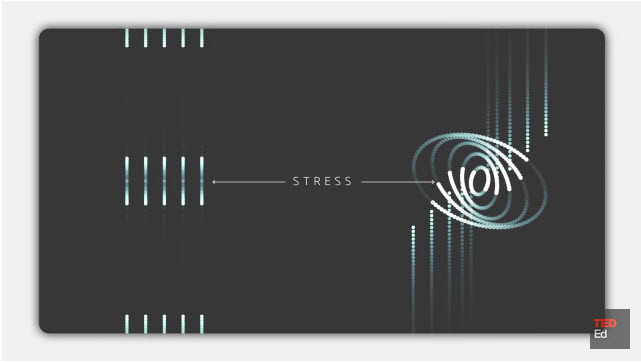
\includegraphics[width=400bp]{geometria-ted-ed-tensor-01.jpg}
\caption{Vídeo TED-Ed sobre vetores e tensores (\url{https://www.youtube.com/watch?v=ml4NSzCQobk}) com legendas em Português.}
\label{\detokenize{GE101-E:fig-geometria-ted-ed-tensor-01}}\label{\detokenize{GE101-E:id7}}
\end{figure}


\subsection{Campos vetoriais}
\label{\detokenize{GE101-E:campos-vetoriais}}
Muitas leis naturais podem ser descritas por equações que envolvem vetores. Estudar estas equações permite entender os fenômenos associados. Neste contexto, o conceito de \index{campo vetorial}campo vetorial desempenha um papel fundamental. Basicamente, um campo vetorial é uma maneira de, a cada ponto do plano, atribuir um vetor. A  \hyperref[\detokenize{GE101-0C:fig-geometria-flechas-03}]{\Fref{\detokenize{GE101-0C:fig-geometria-flechas-03}}} e a \hyperref[\detokenize{GE101-0C:fig-geometria-flechas-08}]{\Fref{\detokenize{GE101-0C:fig-geometria-flechas-08}}} exibem exemplos de campos vetoriais: a cada ponto do mapa estabelece-se um vetor que representa a velocidade do vento naquele ponto (em um dado instante).

Para saber um pouco mais sobre campos vetoriais e de como eles são usados para se criar equações que descrevem fenômenos, recomendamos a animação "CAOS II: CAMPO DE VETORES - A CORRIDA DOS LEGOS"
\url{http://www.chaos-math.org/pt-br/caos-ii-campos-de-vetores} produzido por Jos Leys, Étienne Ghys e Aurélien Alvarez, com áudio em Português e duração de 13 minutos aproximadamente.

\begin{figure}[H]
\centering
\capstart

\noindent\includegraphics[width=400bp]{{geometria-campo-vetorial-caos-01}.jpg}
\caption{Entendendo campos vetoriais com LEGO (\url{http://www.chaos-math.org/pt-br/caos-ii-campos-de-vetores}).}\label{\detokenize{GE101-E:fig-coloque-aqui-o-nome}}\label{\detokenize{GE101-E:id8}}\end{figure}

Este vídeo é uma das nove animações que compõem o filme CAOS. Os tópicos tratados incluem \index{sistemas dinâmicos}sistemas dinâmicos, o \index{efeito borboleta}efeito borboleta e a \index{teoria do caos}teoria do caos. O conteúdo é acessível ao público em geral e certamente você irá gostar e apreciar o uso e a importância de vetores nas várias questões abordadas nos vídeos.


\subsection{Um pouco da história dos vetores}
\label{\detokenize{GE101-E:um-pouco-da-historia-dos-vetores}}
Ao contrário de muitos assuntos que você já estudou, a abordagem moderna de vetores como apresentada neste capítulo (e seus desdobramentos como vistos nos cursos universitários de cálculo vetorial) é relativamente recente. Dois nomes se destacam: Josiah Willard Gibbs (1839\textendash{}1903) e Oliver Heaviside.

\begin{figure}[H]
\centering
\capstart

\noindent\includegraphics[width=350bp]{{historia-01}.jpg}
\caption{Gibbs e Heaviside (Fonte: Wikimedia Commons)}\label{\detokenize{GE101-E:fig-historia-01}}\label{\detokenize{GE101-E:id9}}\end{figure}

Gibbs foi um cientista americano que fez contribuições importantes para as áreas de Física, Química e Matemática. Em 1901, Gibbs ganhou a medalha Copley da Real Sociedade de Londres por ser o primeiro a aplicar a segunda lei da termodinâmica em uma discussão exaustiva da relação entre energia e capacidade térmica, elétrica e química para trabalho externo. Gibbs usou métodos vetoriais para determinar as órbitas de planetas e cometas. Heaviside foi um físico-matemático britânico autodidata com contribuições nas áreas de Matemática e Telecomunicações. Heaviside empregou seu cálculo vetorial para estudar eletromagnetismo e, em particular, simplificar as equações de Maxwell que fazem parte da função do eletromagnetismo clássico, da teoria quântica de campos, da ótica clássica e dos circuitos elétricos.

Algumas "ideias vetoriais"{} já eram conhecidas bem antes de Gibbs e Heaviside. Por exemplo, a regra do paralelogramo (das velocidades) já aparecia no tratado de Mecânica de Heron de Alexandria (c. 10 a.C.\textendash{}c. 70 a.C.). Na sua obra \textit{Principia Mathematica} (1687),  Isaac Newton (1642-1727) trabalhou intensamente com grandezas hoje consideradas vetoriais tais como velocidade e força mas sem, contudo, usar o conceito de vetor.

Segundo o historiador Michael J. Crowe, o início da análise vetorial se deu com o matemático alemão Carl Friedrich Gauss (1777-1855) que, em 1831, publicou uma justificativa geométrica para os números complexos. Entre Gauss e Gibbs/Heaviside, participaram da história dos vetores: William Rowan Hamilton (1805-1865) que introduziu a classificação de grandezas em escalares e vetoriais e inventou os \index{quatérnios}quatérnios; Hermann Grassmann (1809-1877); Peter Guthrie Tait (1831-1901) e James Clerke Maxwell (1831\textendash{}1879). Uma história mais completa dos vetores pode ser encontrada no livro \textit{A History of Vector Analysis: The Evolution of The Idea of A Vectorial System} de Michael J. Crowe, publicado pela editora Dover em 1985.


\subsection{Formigas do deserto, abelhas e vetores}
\label{\detokenize{GE101-E:formigas-do-deserto-abelhas-e-vetores}}
Quando uma formiga típica procura comida, marca seu caminho com ferormônios. Ao encontrar alimento, ela se guia de volta para o formigueiro farejando a trilha que marcou. Mas e a formiga do deserto? Se um vento levar embora a areia marcada, será que ela fica perdida? Cientistas \citet{wehner1981} descobriram que as formigas do deserto não ficam perdidas, pois elas se orientam por um método usado por marinheiros antigamente, o \index{cálculo de posição}cálculo de posição. Esse método se baseia em um procedimento matemático chamado de \index{integração por caminhos}integração por caminhos. O cérebro da formiga realiza naturalmente um cálculo que fornece para a formiga a direção, o sentido e a distância exata (um vetor) permitindo assim que a formiga volte em linha reta ao formigueiro. Integração por caminhos é um assunto que engenheiros e matemáticos estudam nas aulas de cálculo da faculdade. Parece que para aprender certas coisas não seria tão ruim ter cérebro de formiga!

\begin{figure}[H]
\centering
\capstart

% \noindent\includegraphics[width=300bp]{{audio-formigas-animation}.png}
\caption{Texto e animação adaptados de \citet{gomes2010}}\end{figure}

E como as formigas sabem em que direção estão andando? Há evidências de que elas usam o sol como referência. Outro pesquisador (Santchi) percebeu isso através de outra experiência interessante. Enquanto uma formiga do deserto seguia seu caminho, ele posicionou um anteparo de um dos lados da formiga impedindo que o sol batesse nela. Do outro lado da formiga, ele colocou um espelho de forma a refletir o sol na direção do inseto. Para a formiga era como se o sol houvesse "mudado de lado". Imediatamente a formiga fez meia volta e começou a caminhar na direção oposta. Para mais informações sobre o tema, recomendamos \citep{gomes2010} e as referências citadas.

Outros animais também "usam"{} vetores em suas vidas. Abelhas, por exemplo, fazem um tipo de dança para comunicar às companheiras uma fonte de alimentação. A direção e sentido da dança dá a direção e sentido da localização da fonte de alimento e a duração da dança especifica a distância. O documentário "A Dança das Abelhas"{} de Andrew Quitmeyer e Tucker Balch (com legendas em Português) dá mais detalhes sobre o assunto.

\begin{figure}[H]
\centering
\capstart

\noindent\includegraphics[width=300bp]{{geometria-abelhas-01}.png}
\caption{Vetores e abelhas \url{https://youtu.be/RGXyhqKsKQk}.}\label{\detokenize{GE101-E:fig-abelhas}}\label{\detokenize{GE101-E:id11}}\end{figure}


\subsection{Vetores para além do plano}
\label{\detokenize{GE101-E:vetores-para-alem-do-plano}}
Enquanto que nosso estudo se concentrou nos vetores do plano (\({\mathbb R}^{2}\)), o conceito de vetor pode ser estendido para o espaço (\({\mathbb R}^{3}\)), para o \index{hiperespaço}hiperespaço (\({\mathbb R}^{n}\)) e além. A \hyperref[\detokenize{GE101-E:fig-vetor-no-espaco}]{\Fref{\detokenize{GE101-E:fig-vetor-no-espaco}}}, por exemplo, ilustra o vetor cujas extremidades são dois vértices de um cubo.

\begin{figure}[H]
\centering
\capstart

% \noindent\includegraphics[width=200bp]{{geometria-vetor-no-espaco}.png}
\caption{Um vetor no espaço \({\mathbb R}^{3}\).}\label{\detokenize{GE101-E:fig-vetor-no-espaco}}\label{\detokenize{GE101-E:id12}}\end{figure}

Como no caso do plano, um vetor no espaço também representa direção, sentido e módulo e ele pode ser descrito algebricamente por suas coordenadas, como ilustra a \hyperref[\detokenize{GE101-E:fig-coordenadas-3d}]{\Fref{\detokenize{GE101-E:fig-coordenadas-3d}}} para o caso do vetor \(\vec{u} = (1, 2, 3)\).

\begin{figure}[H]
\centering
\capstart

% \noindent\includegraphics[width=350bp]{{geometria-coordenadas-3d-01}.png}
\caption{O vetor \(\vec{u} = (1, 2, 3)\) no espaço \({\mathbb R}^{3}\).}\label{\detokenize{GE101-E:fig-coordenadas-3d}}\label{\detokenize{GE101-E:id13}}\end{figure}

Enquanto que não conseguimos enxergar flechas em \({\mathbb R}^{4}\), \({\mathbb R}^{5}\), …, podemos trabalhar com vetores nestes espaços por meio de suas coordenadas. Assim, por exemplo, \(\vec{u} = (1, 0, -5, 7)\) e \(\vec{v} = (2, 3, 5, 9)\) são dois vetores de \({\mathbb R}^{4}\). Não podemos visualizá-los, mas podemos somá-los e multiplicá-los por um número real. Vetores em \({\mathbb R}^{n}\), mesmo sem uma contrapartida visual, são extremamente úteis. Existe uma área da Matemática dedicada ao assunto, \index{Álgebra Linear}Álgebra Linear, com aplicações em Biologia, Economia, Computação Gráfica, Engenharia, Física, Matemática, Química, entre outras. Aqui está um exemplo em Ecologia. Segundo {[}Valentim-2005{]}, faz parte do trabalho do ecólogo procurar agrupar amostras de mesmas características ou associar espécies em comunidades com o objetivo de descrever, de maneira clara e sintética, a estrutura de um ecossistema. Neste contexto, uma prática é coletar medidas das espécies, como ilustra a \hyperref[\detokenize{GE101-E:fig-ecologia}]{\Fref{\detokenize{GE101-E:fig-ecologia}}} para o caso de um peixe.

\begin{figure}[H]
\centering
\capstart

\noindent\includegraphics[width=270bp]{{geometria-ecologia-01}.jpg}
\caption{Medidas morfométricas de um peixe. Fonte: \citet{pinheiro2016}}
\label{\detokenize{GE101-E:fig-ecologia}}\label{\detokenize{GE101-E:id14}}\end{figure}

Para estudos de semelhança, agrupamento e ordenação, essas medições são registradas em um vetor em \({\mathbb R}^{12}\),
\begin{equation*}
\begin{split}\text{(AB, AC, APCd, AM, CCa, CNPt, CPCd, CP, LB, LNPt, LC, LPCd)},\end{split}
\end{equation*}
para posterior processamento usando técnicas da Álgebra Linear.

Um outro exemplo em Ecologia, este em \({\mathbb R}^{3}\) que você pode visualizar e brincar se refere à simulação do voo de um bando de pássaros. Para isto, acesse o site \url{http://black-square.github.io/BirdFlock/} e, na simulação, clique em "Settings"{} (Configurações) e, depois, em "Algorithm Explanation Vectors"{} (Vetores para Explicação do Algoritmo) para visualizar os diferentes tipos de vetores usados na simulação (na \hyperref[\detokenize{GE101-E:fig-passaros}]{\Fref{\detokenize{GE101-E:fig-passaros}}}, as extremidades iniciais de todos os vetores estão nas posições dos pássaros). Dica: clique em um dos pássaros para acompanhá-lo e use a roda do mouse para se aproximar e pressione a tecla T para fazer com que a rotação da câmera acompanhe o movimento do pássaro. Você pode usar as teclas A, S, D, W, Q e E para navegar pelo cenário.

\begin{figure}[H]
\centering
\capstart

\noindent\includegraphics[width=300bp]{{geometria-passaros-01}.jpg}
\caption{Simulação do voo de um bando de pássaros usando vetores (\url{http://black-square.github.io/BirdFlock/}).}\label{\detokenize{GE101-E:fig-passaros}}\label{\detokenize{GE101-E:id15}}\end{figure}

Basicamente, o que a simulação faz é coordenar o movimento de cada pássaro de modo a: (1) evitar um aglomerado local muito intenso, pois um pássaro não quer se colidir com outro; (2) seguir a direção e sentido do movimento dos pássaros em sua volta, pois um pássaro não quer ficar sozinho uma vez que, assim, ele seria uma presa fácil para um predador em potencial; (3) mover para a posição média dos pássaros em sua volta pelo mesmo motivo de (2).


\ifnum\aluno=1
\clearpage
\else
\notasfinais
\fi

\anexo{Anexo 1: Corrida de Vetores}

\begin{figure}[H]
\centering
\capstart

\noindent\includegraphics[width=.85\textheight,angle=90,origin=c]{{geometria-cv-02}.jpg}
\end{figure}

\begin{figure}[H]
\centering
\capstart

\noindent\includegraphics[width=.85\textheight,angle=90,origin=c]{{geometria-cv-03}.jpg}
\end{figure}

\clearpage

\bibliographystyle{apalike-pt}
\bibliography{../Bibliografia/vetores_bibliografia.bib}

\nocite{*}
